\documentclass[11pt,a4paper,onecolumn,twoside]{article}
\usepackage[french, english]{babel}\frenchsetup{og=«, fg=»}

\usepackage{geometry}
\geometry{
	left=1.25cm,
	right=1.25cm,
	top=2cm,
	bottom=2cm,
	headsep=0.75cm,
}

% version du document basée sur la valeur de la constante de structure fine
% α =7,297352566.10^-3
\newcommand{\Version}{7}

% Macros for setting up and presenting this article

% définir le français comme langue
%\usepackage[french]{babel}\frenchsetup{og=«, fg=»}
\usepackage[autolanguage]{numprint} % for the \nombre command
% pour signaler les erreurs de typo
%\usepackage[All]{lua-typo}
%Hyphenation rules
\usepackage{hyphenat}

\usepackage{tikz,fontspec}
\usepackage{tikz-3dplot}

% fonte pour LuaLaTeX
\usepackage{fontspec}

% ajout des chiffres oldstyle
%\addfontfeature{Numbers={OldStyle,Proportional}}
% pour les formules mathématiques
\usepackage{unicode-math}
\usepackage{amsmath}
%\setmathfont{STIX Two Math}
%\setmainfont{STIX Two Math}
%\usepackage{fancyhdr} 

\usepackage{multicol}

% color
\usepackage{xcolor}
\definecolor{pkcolor}{rgb}{0.0, 0.2, 0.4}  % Blue

\usepackage{titlesec}
\usepackage{titling}
\usepackage{indentfirst}
\usepackage{tabularray}

\usepackage{pgfplots}
\pgfplotsset{compat=1.18}

\usepackage[version=4]{mhchem}
%\usepackage{footnotehyper}
\usepackage{bm}
\usepackage[colorlinks]{hyperref}
\hypersetup{
	colorlinks=true,
	linkcolor=blue,
	filecolor=magenta,      
	urlcolor=cyan,
	citecolor=violet,
	pdftitle={},
	pdfpagemode=FullScreen,
}
\usepackage{afterpage}


% shortcuts
\newcommand{\PQ}{plénodynamique quantique}
\newcommand{\MQ}{mécanique quantique}
\usepackage{xfrac}
%\usepackage{units}
% belles fractions
\newcommand{\R}[2]{\sfrac{#1}{#2}}
\newcommand{\Rv}[4]{\raisebox{0.3ex}{${\scriptscriptstyle #1}$}$\frac{#2}{#3}#4$}
\newcommand{\Ru}[4]{\raisebox{0.7ex}{${\scriptscriptstyle #1}$}$\sfrac{#2}{#3}#4$}


% headers
\usepackage{fancyhdr}

% Redéfinition du style du numéro de page pour les headers
\newcommand{\thepagefhf}{%
	\begingroup
	\setlength{\fboxsep}{3pt} % Espace entre le chiffre et le bord du carré
	\colorbox{pkcolor}{\color{white}\sffamily\small\bfseries\arabic{page}}%
	\endgroup
}

\newcommand{\titlehead}{
	\color{pkcolor}\sffamily\small\bfseries{Plénodynamique quantique}
}

% Redéfinition du style 'plain' (utilisé sur la 1ère page) pour qu'il soit vide
\fancypagestyle{plain}{
	\fancyhf{} % Supprime tout (en-tête et pied de page)
	\renewcommand{\headrulewidth}{0pt} % Enlève la ligne si présente
}

\pagestyle{fancy}
\fancyhf{}
\fancyhead[RO,LE]{\titlehead}
\fancyhead[LO,RE]{\thepagefhf}
% enlève le pied de page
\cfoot{}
% trait horizontale
\renewcommand{\headrulewidth}{1pt}
\renewcommand{\headrule}{\hbox to\headwidth{\color{pkcolor}\leaders\hrule height \headrulewidth\hfill}}



% Title and subtitle
\newcommand{\titlefont}{\bfseries\color{pkcolor}\fontsize{20}{24}\sffamily\selectfont}


% Redefine headers title
\makeatletter

\newcommand{\@subtitle}{}
\newcommand{\subtitle}[1]{\renewcommand{\@subtitle}{#1}}
\newcommand{\subtitlefont}{\bfseries\color{pkcolor}\fontsize{16}{18}\sffamily\selectfont}

\def\@maketitle{
	\begingroup
		{\raggedright\titlefont\@title\par\vskip8pt}
		{\raggedright\subtitlefont\@subtitle\par\vskip8pt}
		{\normalsize\sffamily\raggedright\@author\hfill{Version\,: \Version}\par}
		{\raggedright\sffamily\selectfont\@date\par\vskip18pt}
	\endgroup
}
\makeatother

% redefine section
\setcounter{secnumdepth}{5}

\titleformat{\section}[hang]
	{\color{pkcolor}\sffamily\large\bfseries}
	{\thesection.}
	{0.5em}
	{\uppercase}

\titleformat{name=\section,numberless}[hang]
	{\color{pkcolor}\sffamily\large\bfseries}
	{}
	{0em}
	{\tikz\draw[pkcolor, fill=pkcolor] (0,0) rectangle (1.25ex, 1.25ex); \hspace{2.5pt}\uppercase}

\titleformat{\subsection}[hang]
	{\color{pkcolor}\sffamily\bfseries}
	{\thesubsection.}
	{0.5em}
	{}     

\titleformat{\subsubsection}[block] % You may change it to "runin"
	{\color{pkcolor}\small\sffamily\bfseries\itshape}
	{\thesubsubsection.}
	{0.5em}
	{} % If using runin, change #1 to '#1. ' (space at the end)    

\titleformat{\paragraph}[runin]
	{\small\bfseries}
	{}
	{0em}
	{} 


% citation

% mise en exergue sympa
\usepackage{awesomebox}
\usepackage[most]{tcolorbox}
\usepackage{varwidth}
\tcbuselibrary{most}
\newtcolorbox{mybox}[2][]{enhanced,
	before skip=2mm,after skip=2mm,
	colback=black!5,colframe=black!50,boxrule=0.2mm,
	attach boxed title to top left={xshift=1cm,yshift*=1mm-\tcboxedtitleheight},
	varwidth boxed title*=-3cm,
	boxed title style={frame code={
			\path[fill=tcbcolback!30!black]
			([yshift=-1mm,xshift=-1mm]frame.north west)
			arc[start angle=0,end angle=180,radius=1mm]
			([yshift=-1mm,xshift=1mm]frame.north east)
			arc[start angle=180,end angle=0,radius=1mm];
			\path[left color=tcbcolback!60!black,right color=tcbcolback!60!black,
			middle color=tcbcolback!80!black]
			([xshift=-2mm]frame.north west) -- ([xshift=2mm]frame.north east)
			[rounded corners=1mm]-- ([xshift=1mm,yshift=-1mm]frame.north east)
			-- (frame.south east) -- (frame.south west)
			-- ([xshift=-1mm,yshift=-1mm]frame.north west)
			[sharp corners]-- cycle;
		},interior engine=empty,
	},
	fonttitle=\bfseries,
	title={#2},#1}

% symboles
\usepackage{pifont}% http://ctan.org/pkg/pifont
\usepackage[dvipsnames]{xcolor}
\newcommand{\vrai}[1][black]{\textcolor{#1}{\ding{51}}}
\newcommand{\faux}[1][black]{\textcolor{#1}{\ding{55}}}
\newcommand{\vraiV}{\vrai[OliveGreen]}%
\newcommand{\fauxR}{\faux[red]}%
% figure

\usepackage[section]{placeins}
\usepackage{caption, subcaption}
% same as tabular environment
\captionsetup[table]{
	position=top,           % ← c'est la ligne importante
%	skip=10pt,              % espace entre le caption et le tableau
%	labelfont=bf,           % label en gras (Table 1)
	textfont=normal         % texte du caption en normal
}

\usepackage{floatrow}
\usepackage{float}
\usepackage{wrapfig}
\usepackage{graphicx}
\graphicspath{ {./figures/} }


% biblio
\usepackage{csquotes}
\usepackage[
backend=biber,
%style=phys,
sorting=ynt,
citestyle=numeric-comp,
]{biblatex}

\addbibresource{plenodynamique-quantique.bib}

% Nœud
\newtcbox{\vnode}{%
	boxrule=0.4pt,          
	arc=1pt,                
	colback=gray!15,        
	colframe=gray!60,        
	coltext=pkcolor,         
	left=1pt, right=1pt,    
	top=1pt, bottom=1pt,      
	boxsep=0pt,             
	fontupper=\ttfamily\small,
	valign=center,
	nobeforeafter,
	box align=base
}
\newtcbox{\node}{%
	boxrule=0.4pt,          
	arc=1pt,                
	colback=blue!15,        
	colframe=blue!60,        
	coltext=black,         
	left=1pt, right=1pt,    
	top=1pt, bottom=1pt,      
	boxsep=0pt,             
	fontupper=\ttfamily\small,
	valign=center,
	nobeforeafter,
	box align=base
}

%\newcommand{\vvnode}[2]{\vnode{$\rotatebox{180}{S}_#1}{#2}}$}

% Lists

\usepackage{enumitem}

\newcommand{\squarebullet}[1][pkcolor]{%
	\tikz[baseline=0.0ex]{
		\fill[#1] (0,0) rectangle (1.1ex,1.1ex);
	}%
}

\setlist[itemize]{
	%label=\textbullet,        % puce classique
	 label=\squarebullet[pkcolor],   % exemple de puce colorée
}

% Headers
\title{Plénodynamique quantique}
\subtitle{La physique fondamentale de l'univers}
\author{Patrice Karatchentzeff}
\date{5 avril 2026}


\begin{document}
	
	
	\maketitle
	
	\begin{center}
		\begin{minipage}{0.9\textwidth}
			\begin{tcolorbox}[colback=pkcolor!13, arc=3pt, boxrule=0pt, left=6pt,
				right=6pt, top=6pt, bottom=6pt, before skip=0pt, after skip=0pt]
				
				{\fontspec[Scale=1.2]{TeX Gyre Heros}\color{pkcolor}\textbf{Résumé}}
				\vspace*{0.25cm}
				
				La physique fondamentale de l'univers est basée sur une algèbre de Clifford
				de dimension 7 ($Cℓ_{7,0}(\mathbb{R})$), contrainte dimensionnellement, et
				construite fractalement selon une double échelle de temps et de dimension,
				avec une impulsion chirale initiale.
				\vskip 6pt
				
				Notre univers actuel repose sur un éther cristallin dont la maille a la
				moitié de la dimension de Planck. Dans ces conditions, il est possible  de
				reconstruire toutes les lois de la physique, y compris ses constantes, de
				construire les particules élémentaires du modèle standard, d'expliquer
				l'atome, ainsi que la structure de son noyau, tout en
				retrouvant le déterminisme perdu en \MQ. De fait, la \PQ\  est une candidate
				sérieuse à la \textbf{théorie du tout.}
				
				\vspace*{0.25cm}
				{\fontspec[Scale=0.8]{Noto Serif} \textbf{Mots-clés:} plénodynamique quantique, physique théorique, théorie du tout, éther, plenum, thermodynamique, super-fluide, entropie, néguentropie, énergie du vide, mécanique quantique, modèle standard de la physique, log-périodicité, structure fractale, cristallographie, vorespace, algèbre de Clifford, bi-vecteur de Clifford, turbine hélicoïdale, nœuds, théorie des champs, topologie, soliton, masse, charge électrique, charge magnétique, spin, monopole magnétique, effets Aharonov-Bohm et Aharonov-Casher, effet Casimir, chiralité, phonon, phonon de charge et de masse, potentiel vecteur, pseudo-particule, modèle de concurrence charge-gravité (CCG), modèle de l'atome, modèle du noyau atomique, modèle du Big Bang, crise du spin du proton, chenille, principe fondamentale de la dynamique quantifié, constante de Planck, constante de structure fine, facteur de Landé, relativité restreinte, relativité générale, particule-pilote, mesure physique, intrication, déterminisme, nombres magiques, trous noirs, Louis de Broglie. }
			\end{tcolorbox}
		\end{minipage}	
	\end{center}
	
	%\vspace*{0.1cm}
	
	\begin{center}	
		\begin{minipage}{0.8\textwidth}		
			{\fontspec[Scale=1.1]{TeX Gyre Heros}\textbf{Abstract:}}
			\textit{The fundamental physics of the universe is based on a 7-dimensional
				Clifford algebra ($Cℓ_{7,0}(\mathbb{R})$), dimensionally constrained and fractally
				constructed according to a dual scale of time and dimension, with an initial
				chiral momentum.}
			
			\vskip 3pt
			
			\textit{Our current universe rests upon a crystalline ether whose lattice is half the Planck dimension. Under these conditions, it is possible to reconstruct all the laws of physics, including its constants, to build the elementary particules of the standard model, to explain the atom, and its kernel structure, while recovering the determinism lost in Quantum Mechanics. As such, Quantum Plenodynamics (QP) stands as a serious candidate for the \textbf{Theory of Everything}.}
			
			\vspace*{0.25cm}
			{\fontspec[Scale=0.7]{Noto Serif} \textbf{Keywords:} quantum plenodynamics, theoretical physics, theory of everything, aether, plenum, thermodynamics, super-fluid, entropy, negentropy, vacuum energy, quantum mechanics, standard model of physics, log-periodicity, fractal structure, crystallography, vorespace, Clifford algebra, Clifford bivector, helical turbine, knots, field theory, topology, soliton, mass, electric charge, magnetic charge, spin, magnetic monopole, Aharonov-Bohm and Aharonov-Casher effects, Casimir effect, chirality, phonon, charged and massive phonon, vector potential, pseudo-particle, charge-gravity competition model (CGC), atomic model, atomic nucleus model, Big Bang model, proton spin crisis, caterpillar, quantized fundamental principle of dynamics, Planck constant, fine-structure constant, Landé g-factor, special relativity, general relativity, pilot-wave, physical measurement, entanglement, determinism, magic numbers, black holes, Louis de Broglie.
				}
			
			\vspace*{0.25cm}
			
		\end{minipage}
	\end{center}
	\begin{center}
			An English translation is proposed at the end of the French version (on page \ref*{English})
	\end{center}
	
	\vspace*{0.5cm}
	
	% French version		
	\selectlanguage{french}
	\begin{multicols}{2}
	
\section{Introduction}

L'histoire des sciences n'est pas exempte d'injustices. Henri Poincaré,
à qui Einstein a emprunté les outils pour créer la relativité
restreinte, est tombé dans l'oubli, tandis qu'Einstein a reçu la lumière
de tous les projecteurs.

Il en va de même de Louis de Broglie. Beaucoup lui ont reproché de
s'arc-bouter sur une vision réaliste de la physique, en cherchant un
sens derrière les pures abstractions mathématiques de la mécanique
quantique. Il ne lui manquait malheureusement que le langage pour
prouver ses fulgurantes visions. Par une seconde ironie de l'histoire,
ce langage est pourtant né contemporainement à de Broglie : il s'agit de la
géométrie algébrique. Puisse le succès de la plénodynamique quantique
refocaliser les projecteurs sur cet homme dont l'histoire a quasiment
effacé la trace, à l'exception de sa célèbre formule d'équivalence
entre la quantité de mouvement et la fréquence.
\medskip

Les théories physiques ne naissent jamais de rien. Selon Henri
Poincaré \cite{poincare:1902:sh}, le physicien tente
d'extrapoler une théorie à partir de faits expérimentaux. Ce sont deux
traces, deux points, à partir desquels le physicien extrapole une loi.
En réalité, il existe une infinité de manières d'extrapoler une loi, car il y a une infinité de façon de relier deux points expérimentaux. La physique --~du moins jusqu'à la mécanique quantique~--
a toujours postulé la continuité entre les deux points, ainsi que le
principe de moindre action de Maupertuis, qui est la façon naturelle
de minimiser l'énergie en passant par le «plus court chemin». Une
autre façon de voir ce principe est l'application du principe du
rasoir d'Ockham: entre toutes les théories possibles, la meilleure
est la plus simple, ce qui est encore une autre façon de dire que la
simplicité va de pair avec la beauté. C'est l'un de deux pivots sur
lequel s'est articulé la création de la plénodynamique quantique. Le
second pivot est celui de l'ancrage dans le réel, cher à Albert
Einstein\footnote{«Je ne peux pas croire que Dieu joue aux dés. [$\ldots$] Si la physique ne représente pas la réalité, elle n'est qu'un divertissement pour mathématiciens.» \cite{EinsteinBorn2005}}. \cite{einstein1949autobiographical} Et à Louis de Broglie. \cite{debroglie1976physique}

Les physiciens ont donc élaboré des théories remarquables à partir de
leurs points expérimentaux. Ils ont ensuite tenté de relier les
théories en partant du principe qu'elles étaient justes, puisqu'elles
fonctionnaient. Une théorie du tout devait donc partir d'une de ces
théories et absorber les autres. Mais pas un instant ils n'ont pensé
que ces théories n'étaient que de très bonnes approximations et qu'à
partir d'une approximation, il n'était pas possible de faire émerger
un modèle plus fin et plus englobant.

Il est possible aussi qu'un autre facteur ait joué. Puisque les
théories «approximatives» étaient très compliquées, alors la théorie
de l'ensemble devait être encore plus compliquée. Il se trouve que
fondamentalement, la théorie de la plénodynamique quantique est partie
du postulat inverse. Le modèle qui structure l'univers, la vie ou la
science, doit être un modèle simple, accessible à tous, au moins dans
son explication générale. Le sens physique doit pouvoir s'expliquer et
se comprendre. Après tout, la physique n'est-elle pas \textit{stricto sensu}
l'application de deux principes élémentaires, la causalité et
l'action-réaction qui, eux aussi, sont parfaitement compréhensibles de
tous? La simplicité, la beauté et le réel. Voici les trois piliers de
la plénodynamique quantique!

C'est la raison pour laquelle ce présent article va être exposé selon
deux angles. Le premier est ontologique et pratique, presque purement
mécanique. On verra d'où sort la théorie, quelles sont les choix qui
ont présidé à sa naissance et à son développement. Le second est plus
mathématique. On verra comment plaquer une topologie et surtout une
métrologie sur le modèle, qui sera évidemment --~et sans surprise~-- une
algèbre de Clifford, confortant le modèle tout en lui permettant
d'ajouter une finesse structurelle qu'une simple analyse ontologique
ne permet pas, comme les formes que peuvent prendre les particules
élémentaires du modèle standard.

Cependant, la plénodynamique ne sort pas pour autant d'un chapeau et
elle prend naissance à partir des résultats expérimentaux fournis par
la mécanique quantique. Elle aurait sans doute pu se fonder sur des
grandeurs extraites de la gravité, mais par une sorte de réflexe
d'échelle, ce qui ne manque pas d'ironie pour une théorie fractale,
l'idée s'est d'abord cristallisée autour des structures les plus
petites de la physique. Ce n'est pas le moindre des paradoxes que de
construire une Physique Fondamentale de l'Univers à partir de
résultats de physiques approximatives. En réalité, la boucle est
bouclée, au sens où la plénodynamique quantique se base bien sur des
valeurs expérimentales --~les fameux deux points de départ~--, mais
cette fois sans en omettre aucun.

Si la première partie se veut plus littéraire, elle ne s'adresse pas
pour autant à un public novice en physique. Elle postule une
connaissance générale de toute la physique actuelle. Ce n'est pas
innocent: la plénodynamique quantique contient en germe toute la
physique!
\vfill\pagebreak
\clearpage

\section{De l'existence d'une structure du vide}

\vspace*{-0.8cm}
\begin{center}
	\begin{longtblr}[
		%theme=widecaption 
		caption={\footnotesize{\textbf{Énergie des particules élémentaires}}},
		%label = {tblr:4-2},
		]{
			colspec={Q[c, co=1] Q[c, co=1] },
			rowspec={Q[m]},
			row{odd}={bg=blue!10!white},
			row{1}={c,mode=text,fg=white,bg=pkcolor, cmd=\textbf}, %cmd=\textbf, blue!80!orange
			rowsep=2pt, colsep=3pt,
			vline{2-Y} = {1}{0.3pt,gray!50},
			vline{2-Y} = {2-Z}{0.3pt,gray!30},
			hline{Z} = {0.1pt,blue},
			% nombre de col début et fin qui apparaissent à chaque page
			% 1 pour le titre par exempel
			rowhead = 1, %rowfoot = 1, 
		}
		Particules               &   Masse                    \\
		Photon                   &    0                       \\
		Gluon                    &    0                       \\
		Neutrino électronique    &    < 0,8 $eV/c^2$          \\
		Neutrino muonique        &    < 0,17 $MeV/c^2$        \\
		Électron                 &    0,511  $MeV/c^2$        \\
		Quark up (u)             &    $\approx$ 2,2 $MeV/c^2$ \\
        Quark down (d)           &    $\approx$ 4,7 $MeV/c^2$ \\
		Neutrino tauique         &    < 18,2 $MeV/c^2$        \\
		Muon                     &    105,7 $MeV/c^2$         \\
		Quark strange (s)        &    $\approx$ 95 $MeV/c^2$  \\
		Quark charm (c)          &    $\approx$ 1,28 $GeV/c^2$\\
		Tau                      &    1,77 $GeV/c^2$          \\
		Quark bottom (b)         &    $\approx$ 4,18 $GeV/c^2$\\
		Boson W                  &    80,4 $GeV/c^2$          \\
		Boson Z                  &    91,2 $GeV/c^2$          \\
		Boson de Higgs           &    125,1 $GeV/c^2$         \\
		Quark top (t)            &    $\approx$ 173 $GeV/c^2$ \\
	\end{longtblr}
\end{center}
\vspace*{-0.2cm}
\begin{center}
\begin{tikzpicture}
	\begin{axis}[
		width=0.95\columnwidth,          % <-- largeur exacte de la page
		height=0.55\columnwidth,     % hauteur proportionnelle (tu peux ajuster)
		%width=14cm,
		%height=9cm,
		xlabel={Masse (m)},
		ylabel={},
		title={Courbe logarithmique des énergies},
		xmajorgrids=true,
		ymajorgrids=true,
		grid style=dashed,
		ymode=log,                  % <--- échelle logarithmique sur l'axe y
		log basis y=10,
		ymin=0.1,                   % pour éviter le log(0)
		ymax=2e11,
		xlabel style={font=\small},
		ylabel style={font=\small},
		title style={font=\bfseries},
		tick label style={font=\small},
		legend pos=south east,
		]
		
		% Données (x = indice, y = valeur)
		\addplot[
		color=blue,
		thick,
		mark=*, 
		mark size=1.5pt,
		] coordinates {
			(0,0)
			(1,0)
			(2,0.8)
			(3,1.70E5)
			(4,5.11E5)
			(5,2.20E6)
			(6,4.70E6)
			(7,1.82E7)
			(8,1.06E8)
			(9,9.50E7)
			(10,1.28E9)
			(11,1.77E9)
			(12,4.18E9)
			(13,8.04E10)
			(14,9.12E10)
			(15,1.25E11)
			(16,1.73E11)
		};
		
		\legend{Courbe logarithmique}
		
	\end{axis}
\end{tikzpicture}
\end{center}
\vspace*{-0.5cm}

Les masses des particules élémentaires du modèle standard de la
physique font clairement apparaître une dispersion log-périodique. Il
existe donc un élément générateur qui suit une loi normale permettant
de reconstituer les particules élémentaires. Cet élément dépend \textit{a
	minima} d'une distance et d'un temps (structure bi-échelle) et suit une
loi fractale.

Il est raisonnable de penser que cet élément est la structure du vide. 

\begin{mybox}[breakable,colback=blue!10, colbacktitle=pkcolor]{Postulat 1}
Le vide n'est pas vide, mais est fabriqué à partir d'un élément unique.
\end{mybox}
\medskip

De façon assumée, la plénodynamique quantique part \textit{a contrario} des
idées reçues. L'éther existe et on va le construire. Einstein, qui a
démontré que l'éther luminifère, le fluide du \textsc{xix}\ieme\ siècle, n'existait
pas, n'y était d'ailleurs pas \textit{stricto sensu} opposé. À l'Université de
Leyde, le 5 mai 1920, il déclara \cite{einstein1920ether}:«En
résumé, nous pouvons dire que d’après la théorie de la relativité
générale, l’espace est doté de propriétés physiques; dans ce sens,
par conséquent, un éther existe. Selon la théorie de la relativité
générale, un espace sans éther est inconcevable, car dans un tel
espace, non seulement il n’y aurait aucune propagation de la lumière,
mais aucune possibilité d’existence pour des règles et des horloges,
et, par conséquent, aucune distance spatio-temporelle au sens de la
physique.» La physique moderne «sent» d'ailleurs qu'il y a bien
quelque chose, comme la mousse quantique de la gravité quantique à
boucles. Ici, on va franchir un pas de plus et construire un modèle
mécanique et thermodynamique de l'espace, en lui donnant une substance
réelle. C'est, en quelque sorte, un retour au source: l'éther n'est
pas un fluide luminifère, c'est un cristal luminifère.


\section{Le modèle du vide: le plenum}

Maintenant que l'existence d'une structure du vide est postulé, il est
capital de modéliser cette structure.

La première réflexion qui vient à l'esprit est que si le vide est
constitué d'un élément générateur, le vide n'existe pas. Tout le vide
est constitué de ces éléments.

\begin{mybox}[breakable,colback=blue!10, colbacktitle=pkcolor]{Postulat 2}
Le vide n'existe pas. Tout le vide est rempli d'éléments joints.
\end{mybox}
\medskip

Le vide n'étant plus vide, et pour éviter toute confusion, on
appellera désormais ce vide un plenum (du latin: assemblée pleine).
Une conséquence immédiate est que, puisque l'élément trouvé est
générateur, il est premier. Il n'existe pas d'élément plus petit. Il
ne peut donc être écrasé. L'élément est rigide.

\begin{mybox}[breakable,colback=blue!10, colbacktitle=pkcolor]{Postulat 3}
Le plenum est rigide.
\end{mybox}
\medskip

Techniquement, le plenum ressemble donc à un cristal. Il a une maille
--~l'élément générateur~-- et une rigidité.

Le plenum est donc topologiquement quantifié.

\section{Le modèle de l'élément générateur du plenum: le vorespace}
	
Il est temps de s'occuper de l'élément générateur, afin de
le modéliser.

Techniquement, toujours selon Poincaré, n'importe quel objet à deux dimensions
d'échelle, une d'espace et une de temps, devrait pouvoir convenir. On
pourra toujours extrapoler une loi plus ou moins compliquée
pour coller au modèle (qui, \textit{in fine}, doit engendrer une particule du
modèle standard). La continuité du plenum élimine cependant tout objet
qui ne soit pas capable de le remplir pleinement, par répétions, comme
un objet circulaire ou sphérique.

C'est ici que le principe du rasoir d'Ockham va servir. L'idée est de trouver
l'objet \textbf{réel} le plus simple, qui construit la loi la plus simple et
qui mène à la création des particules élémentaires.

Après quelques tâtonnements qui ont conduit à des impasses de
sur-complexité de loi\footnote{La difficulté principale est de rendre
la propriété de spin si elle n'est pas intrinsèque.}, le plus simple a
été de postuler l'existence d'un objet qui possède déjà certaines
propriétés des particules élémentaires.

On cherche donc un objet \textbf{réel} ayant au moins intrinsèquement la
propriété de spin et de charge électrique. Cet objet existe: le plus
simple est le bi-vecteur de Clifford de dimension 3, auquel on ajoute
une vitesse de rotation permettant d'assurer la chiralité, et donc la
charge électrique. La vitesse nous apporte en plus, mécaniquement,
l'unité de temps de la loi fractale.

On pourrait donc se précipiter sur cet objet, nommé $S_3$ dans l'algèbre
de Clifford, et construire notre plenum avec ce bi-vecteur. Toutefois, il serait
dommage de ne pas profiter d'une propriété de cette algèbre
géométrique. Elle postule en effet l'existence de 7 nœuds stables, des
v-sphères, nommées $S_1$ à $S_7$, chacune se construisant sur la
combinaison du nœud précédent. C'est intrinsèquement une loi
fractale. 

Le fait donc que $S_3$ soit l'objet le plus simple répondant à
notre problématique et qu'il suive déjà une loi fractale d'ordre 7 nous
pousse, toujours à cause du principe du rasoir d'Ockham, à choisir aussi cette loi
fractale comme candidate à la loi recherchée. Il se trouve que
l'algèbre de Clifford de dimension 7 reste une algèbre de Clifford,
même si on la contraint dimensionnellement, ce qui est compatible avec
notre contrainte de départ.

\begin{mybox}[breakable,colback=blue!10, colbacktitle=pkcolor]{Postulat 4}
L'élément générateur du plenum est un bi-vecteur de Clifford de
dimension 3, doté d'une vitesse de rotation et contraint
dimensionnellement. Il suit la loi fractale de l'algèbre de
Clifford de dimension 7.
\end{mybox}
\medskip

Pour faire de la mécanique avec cet objet, il est nécessaire de bien
comprendre ce qu'il est, comment il peut être représenté et comment il
fonctionne.

Techniquement, l'objet de base est composé de deux vecteurs ayant de
grandes libertés de mouvement, sept en tout. Il est très particulier
au sens où il est auto-contraint. Changer une dimension d'une partie
de l'objet (au sens d'une capacité engendrée par un des sept degrés de liberté)
change la forme globale de l'objet. Techniquement, cet objet a un module de Poisson valant $-1$, donc un module d'élasticité nul et un module de torsion infini. Il est infiniment déformable à rayon constant, mais non pliable.

Globalement, l'objet $S_3$ est une double-hélice intriquée qui forme une
turbine. La turbine possède 128 états de configuration qui lui
permettent de passer de l'état de turbine poussant dans un sens à
l'état de turbine poussant dans l'autre. Enfin, la turbine a sept
pas de vis. La contrainte de l'objet fait qu'il reste toujours une
turbine au cours de son évolution dans les 128 états possibles. On
peut voir les deux hélices emmêlées comme deux objets indépendants
seulement dans les états extrêmes des turbines. Chaque état
correspond à une mobilisation des 7 degrés de libertés possibles.
\end{multicols}

\vspace*{-1cm}
\begin{center}
	\begin{longtblr}[
		%theme=widecaption 
		caption={\footnotesize{\textbf{Description du vorespace}}},
		%label = {tblr:4-2},
		]{
			colspec={Q[2cm,c,m] Q[c,m] Q[c,m] Q[2cm,c,m] Q[2cm,c,m] Q[3cm,c,m] Q[3cm,c,m]},
			rowspec={Q[m]},
			row{odd}={bg=blue!10!white},
			row{1}={c,mode=text,fg=white,bg=pkcolor, cmd=\textbf}, %cmd=\textbf, blue!80!orange
			rowsep=2pt, colsep=3pt,
			vline{2-Y} = {1}{0.3pt,gray!50},
			vline{2-Y} = {2-Z}{0.3pt,gray!30},
			hline{Z} = {0.1pt,blue},
			% nombre de col début et fin qui apparaissent à chaque page
			% 1 pour le titre par exempel
			rowhead = 1, %rowfoot = 1, 
		}
		Degrés de liberté       &   Objet   & États  & Nombre d'états & Sens de rotation & Forme & Hélice    \\
	    3                       &    turbine aspirante  &    1 à 19  &     20   &       chiral &              cône vissé (sept pas)  &        une seule hélice tourne \\
	    4 à 7            &         idem        &         20 à 61   &   42     &     chiral     &           aplatissement         &         deux \\
	    idem     &                blocage       &        61 à 65    &   4      &      nul         &         disque obstruant    &           aucune \\
	    idem        &            turbine soufflante   &  66 à 107  &   42   &      anti-chiral &          étirement    &                  deux \\
	    3                  &        idem        &        108 à 127  &  20       &   anti-chiral     &     cône vissé inversé (sept pas) & une seule (mais l'autre) \\
	    	
	\end{longtblr}
\end{center}
%\end{multicols}

\begin{multicols}{2}

Il y a donc concrètement deux objets stables à 3 dimensions, chacun
soufflant dans une direction opposée, et de forme inversée, formant un
cône, comme une vis à 7 pas. La vis s'écrase dans un premier tas pour
former un disque qui obstrue le passage, puis croît pour former une
nouvelle vis, inversée, comme si le vissage initial traversait le
disque. Il y a clairement un effet miroir au niveau du disque de
blocage. À noter un point capital :\textit{ la transformation de l'état 1 à
l'état 128 se fait à dimension constante.}

Dans un premier temps, il n'est pas nécessaire d'approfondir davantage
les caractéristiques de cet objet extraordinaire, mais on sera
rapidement amené à y revenir. Les positions 21 à 108 vont offrir un
panel exceptionnel de possibilités pour expliquer toute la physique.
Pour construire notre plenum, on n'a besoin que d'un objet réel.
Toujours pour des raisons de simplicité, nous allons donc postuler que
l'objet réel est la turbine de dimension 3 et construire notre plenum
avec cette turbine.

On nomme $L_v$ la contrainte dimensionnelle de notre objet. Elle est donc
la plus petite distante de l'univers. Notre bi-vecteur possède de plus
une vitesse de rotation $\omega_v$. Le bi-vecteur n'étant plus tout à fait un
bi-vecteur quelconque avec ces contraintes, on l'appellera désormais
\textbf{vorespace}, par contraction de vortex et d'espace, vortex évoquant bien
l'idée de la turbine.

\begin{mybox}[breakable,colback=blue!10, colbacktitle=pkcolor]{Postulat 5}
La maille du plenum est un vorespace, un bi-vecteur de Clifford de
dimension 3, ayant une norme de dimension $L_v$, la plus petite des
dimensions, et une vitesse de rotation $\omega_v$, appliquée uniquement à
l'un des bi-vecteurs.
\end{mybox}
\medskip

Techniquement, le vorespace est une turbine à 7~pas de dimension 3.
C'est un objet tri-dimensionnel, chargé électriquement et possédant un
spin de \R{1}{2}.
\medskip

La forme étant globalement un cône, la vision cubique euclidienne de
l'élément générateur de l'espace a donc vécu$\dots$


\section{Le modèle du plenum}

Le plenum est donc un véritable champ physique, contenant en son sein
les trois propriétés fondamentales des particules élémentaires,
contrairement aux trois champs abstraits de l'électrodynamique
quantique.

C'est d'ailleurs une caractéristique de la plénodynamique quantique :
tous les champs sont des champs réels.

Pour respecter le postulat 2, on ne peut pas placer les vorespaces
n'importe comment dans l'espace. Autrement dit, le cristal est
contraint par la forme du vorespace (et réciproquement).

La première contrainte est mécanique, à cause du pas de vis. Si l'on
place deux vorespaces ayant la même chiralité à la suite, ils vont
s'opposer et se bloquer. On peut les voir comme deux roues d'engrenage
consécutives: elles tournent toujours dans des sens opposés. Le
plenum est donc composé de vorespaces à la chiralité alternative.
Physiquement, cela revient à alterner des charges positives et
négatives.

\begin{mybox}[breakable,colback=blue!10, colbacktitle=pkcolor]{Conséquence 1}
Le plenum est électriquement neutre.
\end{mybox}
\medskip

Quel que soit le volume du plenum, si l'on respecte la quantification
de maille, le volume contiendra autant de charges positives que
négatives.
\bigskip

La seconde contrainte est spatiale. Pour ne pas laisser de trou dans
le plenum, deux vorespaces voisins doivent «s'emboîter» (à la
manière d'un tore, s'entend). Si l'on prend l'image de la vis, la tête
de vis et le pied de vis doivent être tête-bêche entre deux places
voisines. Les axes de rotation de deux vorespaces sont donc retournés.
Les spins aussi. Le plenum est donc composés de vorespaces alternant
les signes de spin.

\begin{mybox}[breakable,colback=blue!10, colbacktitle=pkcolor]{Conséquence 2}
Le plenum a un spin de zéro.
\end{mybox}

\subsubsection*{Peut-on imaginer à quoi ressemble le plenum?}

Commençons à une dimension, pour que cela soit plus facile à
visualiser. Le vorespace ressemble à une vis, c'est-à-dire un cône.
Les contraintes précédentes forcent la disposition tête-bêche d'une
succession des cônes, la grande surface du premier épousant la grande
du suivant et donc la petite de la petite du suivant. On a donc une
série de doubles cônes. Visuellement, cela ressemble à une onde. Mais
comme il y a en réalité une (double) hélice qui tourne à l'intérieur,
l'image la plus parlante est celle de$\ldots$ l'ADN.

On gardera le nom, bien que les initiales désignent autre chose. Mais
l'image est belle: c'est l'ADN du plenum. On peut être physicien et
poète, cela n'est pas antinomique!

Bien entendu, le plenum est à trois dimensions, donc le brin d'ADN
doit être adapté. On peut le voir à deux dimensions comme un
empilement joint de brins d'ADN à une dimension. Chaque «contact»
s'effectue selon la même contrainte que celle de la dimension
unitaire. Les grands et les petits «diamètres» ensemble. Il est
difficile d'imaginer l'emboîtement de ces quatre surfaces, car il
s'agit d'une hypersurface. Mais concrètement, c'est l'intersection de
quatre cônes.

Bien entendu, il faut compléter la troisième direction avec un nouveau
brin perpendiculaire, pour finir de remplir le plenum. Les jonctions
deviennent difficilement visualisables.

Le modèle du plenum est terminé.
\medskip

On a bien un modèle à 3 dimensions par construction. Mais le vecteur
de Clifford sous-jacent a une structure potentielle de 7 dimensions.
Le plenum peut être vu comme un gel de 3 dimensions d'un vorespace
à 7 dimensions. Le vorespace a donc en réserve un
potentiel de 4 dimensions. On peut le voir comme «le potentiel du
vide». On le mobilisera bien entendu pour expliquer la nature des
champs électromagnétiques et de gravité.

\section{Le modèle fractal}

L'existence d'une loi fractale pour engendrer les particules
élémentaires du modèle standard est avérée par la log-périodicité des
énergies des particules élémentaires.

Essayons d'en comprendre le mécanisme. L'idée générale est la
reproduction conforme, l'auto-similarité par changement d'échelle.
On part du bi-vecteur, le vorespace, et on obtient un nouveau
bi-vecteur, à l'échelle suivante. Il faut donc prendre deux
vorespaces, chacun jouant le rôle d'un vecteur. La fusion des deux
vorespaces va donner un unique vorespace, mais de taille double. Bien
entendu, la complexité des formes va augmenter de façon exponentielle.
On a déjà du mal à imaginer correctement la turbine de base, donc une
turbine de turbine est déjà presque hors de portée de l'imagination.
L'étape suivante devient bien sûr d'une inextricable complexité. Et
comme on peut aller ainsi jusqu'à sept fois de suite, la forme de la dernière
est au-delà de tout ce qu'il est possible d'imaginer.

Par chance, en choisissant l'algèbre de Clifford comme loi fractale,
il est possible de connaître la \textit{forme combinée générale} de chacune
des étapes stables, après 7 évolutions (7 coups de vis). Les états sont donc
les nœuds de l'algèbre de Clifford, les v-sphères $S_1$ à $S_7$ et chaque
nœud aura 7 capacités de mouvement, correspondant techniquement aux fibrations. On
explicitera la forme que prendront ces nœuds dans la partie du modèle standard
de la physique.
\medskip

Quoi qu'il en soit, le mode de reproduction suit le modèle suivant:

\begin{itemize}
	\item 7 pas pour fusionner (fractalité temporelle);
	\item objet stable au 8\ieme\ pas (fractalité spatiale);
	\item l'objet stable est caractéristiquement identique au 1\ier\ objet de
	l'échelle inférieure.\footnote{Ce n'est pas tout à fait exact dans le cadre de l'algèbre de Clifford, car l'autosimilarité des différents nœuds suit aussi une loi interne que l'on mettra en évidence un peu plus loin.} 
\end{itemize}


Quand on parle de caractéristiques, il s'agit des propriétés
intrinsèques de l'objet: forme, charge (chiralité), nombre de pas de
vis (7), nombre d'états possibles (128).

Chaque objet est donc spatialement et dimensionnellement doublé par
chaque coup de vis de la fractalité, c'est-à-dire qu'un nœud stable
sera toujours une puissance $2^8$ fois plus grande que le nœud précédent.
Bien entendu, si la contrainte dimensionnelle est imposée, la taille
reste constante. On verra que cette contrainte n'est applicable que
jusqu'à la naissance du plenum et, qu'ensuite, la contrainte
dimensionnelle s'envole. Tout ceci sera explicité dans le modèle
cosmologique du Big Bang.

 \subsubsection*{Comment fusionnent deux vorespaces?}

Pour fusionner deux objets, il faut une zone de contact et un
mécanisme. Cela tombe bien, car on a construit deux vorespaces
consécutifs en contact, avec un mécanisme d'emboîtement: leur pas
de vis. Si l'un tourne, l'autre aussi.

Comment fusionner? Comme il s'agit d'une auto-réplication, les
propriétés de chacun doivent fusionner. Toute l'information de
structure de l'un doit passer à l'autre. C'est toute la beauté du
bi-vecteur: chaque tour de vis exprime le contenu complet de
l'information de sa structure. Un tour faisant $2\pi$, chaque tour
produit un contenu informationnel binaire. Au premier tour, on n'a
qu'une information, au second deux, \textit{etc.} En tout, le vorespace est
constitué de $2^7=128$ formes possibles. Chaque tour de vis entraîne de
façon mécanique un tour de vis du vorespace suivant, ce qui le
contraint à se conformer au vorespace précédent. L'information
circule. Au 7\ieme\ tour de vis, toute la structure du premier vorespace a
été transmise au second. Ils sont identiques. C'est le 8\ieme\ tour qui
provoque véritablement la fusion. Les deux vorespaces ne font alors
plus qu'un. La dimension spatiale a doublé et toutes les informations
de structure respectent ce doublement dans leur dimensionnalité (une
surface aura donc quadruplé): la dimension du nouveau vorespace est
$2L_v$, car la maille est incompressible. Seul reste constant le nombre
de tours de vis, et donc le nombre de formes possibles de la nouvelle
forme: c'est la beauté de la fractalité. On change d'échelle, pas de
forme, donc de propriétés structurelles. La progression étant
exponentielle, on se doute qu'il ne faudra que quelques dizaines de
tour pour attendre l'échelle de la particule.

Bien entendu, le mécanisme de fusion \textit{in se} n'est pas encore décrit:
il sera explicité lorsque de la description du mécanisme de la gravité.

Une conséquence triviale est que

\begin{mybox}[breakable,colback=blue!10, colbacktitle=pkcolor]{Conséquence 3}
	Toute particule élémentaire a une taille proportionnelle à une puissance de deux de la taille du
	plenum, soit $L_v$.
\end{mybox}
\medskip

Il reste à déterminer l'échelle temporelle. Elle est trivialement cachée
dans le mécanisme de vissage. C'est la vitesse de rotation qui impulse
le tempo. La réplication demande 7 tours de vis à la vitesse de
rotation du vorespace. La fusion n'est donc pas instantanée.

C'est là que les choses amusantes commencent$\ldots$ Si l'engrenage formé
par deux vorespaces n'était pas idéal, alors, par effet de bord, il
arriverait un moment où un engrenage s'arrêterait. La communication
dans le plenum serait bloquée. Pour assurer que la communication
puisse se transférer dans tout le plenum, il faut que la résistance
des engrenages soit nulle. Les turbines communiquent donc de façon
parfaite, le transfert est idéal. Par conséquence, il n'y a rien qui ne puisse 
aller plus vite. C'est le temps de transfert le plus rapide. Il est de
bon sens ici de postuler que ce temps est compatible avec c. C'est la
vitesse de propagation de l'information la plus rapide.

Le tic de l'horloge de l'univers est donc le temps de propagation de
toute l'information de structure d'un vorespace à son voisin.

On notera $\omega_v$ la vitesse de rotation du vorespace dans cette
configuration. On peut la voir de différentes manières :

\begin{itemize}
	\item soit déduite de c pour rester compatible avec la relativité
	restreinte;
	\item soit engendrant c en raison des contraintes mécaniques du
	vorespace.
\end{itemize}

En réalité, c'est la seconde qui est vraie, car la structure du plenum
qu'on a laborieusement construite avec des contraintes topologiques
pures ne sort en réalité pas du vide: elle est aussi produite
fractalement. On verra par la suite qu'il s'agit en réalité d'un
héritage de l'ère pré-planckienne, quand l'univers était purement
photonique, avant la réplication d'échelle. c\,~dépend en réalité de
la quantité d'énergie insufflée au départ du système cosmologique.
\medskip

La vitesse de rotation étant aussi une énergie, $\omega_v$ est donc 
l'énergie du vorespace. C'est l'énergie du point zéro. On peut 
la voir comme \textit{l'énergie de structure du vorespace du plenum}.
Le transfert d'information d'un vorespace à l'autre est aussi un
transfert d'énergie. Comme elle est purement mécanique (rotation de la
vis), elle est, par définition, de l'exergie. Toute l'énergie du
premier vorespace a été consacrée au transfert d'information, sans
perte. La dispergie est donc nulle, ce qui est une autre façon
d'énoncer que le système d'engrenages fonctionne sans frottement. On
retrouve l'idée de super-fluidité.

Le modèle est donc à la fois mécanique et thermodynamique. Le
mécanisme étant plus illustrant que réel, le modèle fractal est sans
aucun doute purement thermodynamique.

\begin{mybox}[breakable,colback=blue!10, colbacktitle=pkcolor]{Postulat 9}
Le plenum est géré par une thermodynamique fractale bi-échelle et
réagit comme un superfluide.
\end{mybox}
\medskip

Tout n'est donc qu'exergie dans le plenum. On peut aussi la voir d'un
point de vue informationnel. Le vorespace contient 128 états codés sur
7 v-bits. L'information n'est transférable que par unité de v-bit. Il
faut donc 7 unités de transfert pour recopier toute l'information du
vorespace. On peut donc imaginer le vorespace comme une turbine (qui
gère un flux physique) ou bien une mémoire séquentielle (qui gère un flux
informationnel). L'image des mémoires à bascules ou à registres de la
logique séquentielle est très illustrante.
\medskip

On peut ensuite se poser la question de ce que représente l'exergie de
cette onde. Si l'exergie de structure est bien illustrable au moyen d'un
engrenage, l'exergie de l'onde est plus mystérieuse.

En réalité, tout s'éclaire quand on la traduit sous la forme
informationnelle. Le vorespace est un 7 v-bit, dans lequel est codée
toute son information: chiralité, vitesse de rotation et direction du
spin. Il n'est pas nécessaire de coder le pas de vis, propriété
structurelle du vorespace. L'exergie de l'onde n'est que la transmission
de toutes ces informations au vorespace suivant.

D'un point de vue de Shannon, cette information est une entropie. Ce
qui réconcilie le point de vue «pure exergétique» au point de vue
entropique est le pas: chaque information est transférée sans perte.
La turbine est le moteur et l'entropie le flux.
\medskip

On a donc trouvé le battement de cœur du plenum. Peut-on le calculer?
\begin{equation*}
	t_v = L_v / c
\end{equation*}

Ne connaissant encore rien de la dimension du vorespace, on ne peut
rien dire de plus à ce stade.
\medskip

En conclusion, le modèle fractal du plenum est thermodynamique, basé
sur un échange d'exergie, à dispergie nulle, la maille étant le
vorespace, un bi-vecteur de Clifford de dimension 7, à norme contrainte,
avec une vitesse de rotation constante.

À noter que l'entropie du vorespace, selon Shannon, vaut 7. Le temps
de propagation de l'information est le coût entropique de Shannon, même
si le mécanisme de transfert est purement exergétique.

\section{Quelques propriétés fondamentales du vorespace}
	
Il faut dissiper très rapidement une confusion qui peut émerger de la
structure du vorespace du plenum. La rotation du vorespace lui donne
une énergie. Mais ce n'est pas une énergie mécanisable: c'est une
énergie de \textbf{structure}. Il faut la voir comme l'énergie qui permet la
rigidité (la tension) du plenum, c'est-à-dire l'équilibre du plenum.
Cette remarque topologique permet de comprendre l'erreur de calcul de
l'électrodynamique quantique quand elle trouve une valeur de $10^{120}$ à
l'énergie du vide. Elle compte l'énergie de la structure, comme une
énergie mobilisable. Ce n'est pas le cas: c'est seulement la rigidité
du cristal.

\begin{mybox}[breakable,colback=blue!10, colbacktitle=pkcolor]{Postulat 10}
Le plenum possède une énergie structurelle, non mobilisable. 
\end{mybox}
\medskip

C'est à peine un postulat, car on peut le voir comme une conséquence
de la stabilité du plenum.

On en déduit immédiatement que si le vorespace a une énergie de
structure égale à $\omega_v$, minimale, toute énergie supérieure à $\omega_v$ est
une énergie de masse.

\begin{mybox}[breakable,colback=blue!10, colbacktitle=pkcolor]{Postulat 11}
La propriété de masse découle de la différence de vitesse de rotation
d'un vorespace, d'une valeur supérieure à la valeur de stabilité
$\omega_v$.
\end{mybox}
\medskip

En conséquence, la masse est une perturbation locale de l'état
d'équilibre du plenum. On développera ce point crucial dans le modèle
de la gravité, nécessaire pour créer une dynamique dans le plenum.

\subsection{Dualité onde-corpuscule}

Le modèle thermodynamique du plenum fait émerger une dualité
ontologique. D'une part, la structure, rigide, qui n'est pas sans
rappeler l'idée de corpuscule et d'autre part, le transfert
informationnel, purement ondulatoire.

La dualité onde-corpuscule de de Broglie trouve là sa racine. On
développera plus profondément cette idée quand on détaillera la masse et la compatibilité avec la \MQ.

\subsection{L'auto-réplication, comme modèle du mouvement}

La thermodynamique du plenum redéfinit l'intuition du déplacement
physique. Il ne s'agit plus d'un objet massif --~même si l'on ne peut
pas encore parler d'objet à ce stade, mais faisons-le par anticipation~--
 qui se déplace physiquement, mais le contenu informationnel de
chaque vorespace de l'objet qui se réplique sur chaque vorespace de la
trajectoire de l'objet.

\begin{mybox}[breakable,colback=blue!10, colbacktitle=pkcolor]{Postulat 12}
Tout objet est donc techniquement un \textit{soliton topologique}.
\end{mybox}
\medskip

On note au passage que cela entraîne \textit{de facto} l'impossibilité de
téléporter un objet réel sans que cela ne viole la relativité restreinte. Il
faudrait transférer l'information de chaque vorespace plus vite que
l'information ne circule déjà, et elle circule à la vitesse de la
lumière.

Un pan entier de la littérature de science-fiction vient de
s'écrouler...

Tant que l'on n'aura pas définit proprement les objets, on ne développera pas
davantage la façon dont ils se déplacent concrètement.

\subsection{La masse comme frein à l'entropie informationnelle}

Il découle du modèle thermodynamique du plenum que si le vorespace
possède une masse ($w > w_v$), alors l'exergie de l'onde --~que l'on
appellera désormais \textit{exergie de phase} ou \textit{exergie informationnelle}~-- ne
peut plus se transmettre intégralement. Le surplus de masse agit comme
un frein pour l'onde. Non seulement la vitesse de transfert ralentit,
mais il peut aussi se bloquer si la masse est suffisante. Il existe
donc une vitesse maximale de rotation $\omega_{max}$ qui bloque le transfert
informationnel. On développera amplement cet aspect dans la partie sur
la masse.

Sans trop anticiper sur la compatibilité avec les autres physiques, on
peut d'ores et déjà avancer que le temps de propagation diminue avec
l'augmentation de la masse. C'est la contraposée d'une des lois de la
relativité générale qui stipule que la masse augmente quand le temps
diminue.

Une autre façon de voir les choses est de considérer que l'exergie
partage sa bande passante (fixe) entre l'énergie de rotation et de
translation. Plus la part dédiée à la rotation augmente, plus la part
dédiée à la translation diminue...

On développera plus largement les raisons du blocage du flux
informationnel dans la partie dédiée à la masse et à la gravité.

\subsection{La plénodynamique quantique}

La \textbf{plénodynamique quantique} se veut donc être la thermodynamique du
plenum. Elle est doublement quantifiée, spatialement par la structure
de maille du cristal du vorespace, et temporellement par la
bande-passante exergique de phase.

Il faut maintenant montrer sa capacité à engendrer les particules
élémentaires du modèle standard, en restant compatible avec les
différentes physiques.

\section{La masse et la charge électrique}

\subsection{Introduction}

Avant de passer à la reconsitution du modèle standard, il est nécessaire de bien
comprendre ce qu'est une masse et une charge électrique. Il faudra
ensuite en tirer les conséquences, à savoir la nature de la force de
gravité et de la force électrique. Et enfin, il sera
possible d'entreprendre la construction des particules élémentaires du
modèle standard.

\subsection{La masse}

La masse est définie comme un surplus de vitesse à partir de la
vitesse du vorespace. Techniquement, à cause des contraintes
inter-hélices, ce surplus de vitesse ne permet pas à la turbine de
rester dans sa zone nominale de fonctionnement, c'est-à-dire dans les positions 1 à
20. Elle doit donc aller chercher dans les positions suivantes. Le
flux décroît donc mécaniquement dans la turbine, ce qui explique le
ralentissement du temps.

La masse ne peut donc prendre que 44 positions, entre la position 21
et 64. Si la masse allait plus loin, la rotation commencerait à
s'inverser, et la masse ne serait plus une masse (techniquement, ce
serait une anti-masse, donc de l'anti-matière). À la position 64, la
masse est à son maximum: elle coupe tout le flux de transmission. Sa
vitesse est donc maximale et on l'appellera $\omega_m$.

Une masse peut donc en théorie prendre tous les états entre la
position 21 ($\omega_v + dw$) à la position 63 ($\omega_m$), soit \textbf{42 états discrets
différents}.
\medskip

D'autre part, la masse ne peut pas prendre tous ces états discrets,
car la contrainte de fusion des pales des hélices fait qu'elles
fonctionnent avec une double contrainte systémique: chaque pale a
deux contraintes d'inclinaison et deux contraintes de forme
(épaisseur et surface de la pale (longueur et largeur)). La
contrainte de fusion exige donc que chaque saut se fasse par paire de
contraintes systémiques, car changer de forme implique de changer
l'inclinaison (et vice-versa). La masse influence seulement la forme 
--~et la physique engendrée par la masse se focalisera donc sur cet
aspect. La vitesse de la masse étant une caractéristique externe aux caractéristiques du
plenum, la physique de la masse devra donc être aussi externe à celle
du plenum, dont on a vu qu'elle était purement thermodynamique. La
masse influence donc la forme de la pale pour influencer le flux du
plenum: sa physique sera une \textit{physique du flux}. Elle sera développée
dans la partie sur la gravité.

La masse ne peut donc exploiter que 44 états par paire de deux états.
Deux états finaux sont connus: ce sont les états de blocage complet
du flux. La turbine ressemble alors à un disque. La masse ne peut donc
varier que dans les 42 états précédents, soit 21 paires. Il n'y a pas
de raison que la loi de progression fractale par paliers de 7 ne
s'applique pas non plus à la masse: \textit{elle varie donc selon 7 paliers de 3
paires.}

L'apparition de la de masse s'effectue par un pas de 7 dans les 42 états
suivant les 20 premiers états d'équilibre. On peut calculer la masse
maximale possible du vorespace en gardant l'idée que $\omega_v$ est l'état
d'équilibre. On a donc à distribuer 7 flux correspondant à une partie
qui doit rester toujours à l'équilibre, c'est-à-dire $\omega_v$, soit \R{1}{7}\ieme\ de
$\omega_v$ à chaque fois. En 7 coups, on a donc impulsé 7 fois \R{1}{7}$\omega_v$, soit
$\omega_v$. La vitesse maximale est donc de $2\omega_v$.

On a donc {\boldmath{ $\omega_m = 2 \omega_v$}} 
\vfill
\clearpage

\begin{figure}[H]
	%\captionsetup{width=5cm}
	\centering
	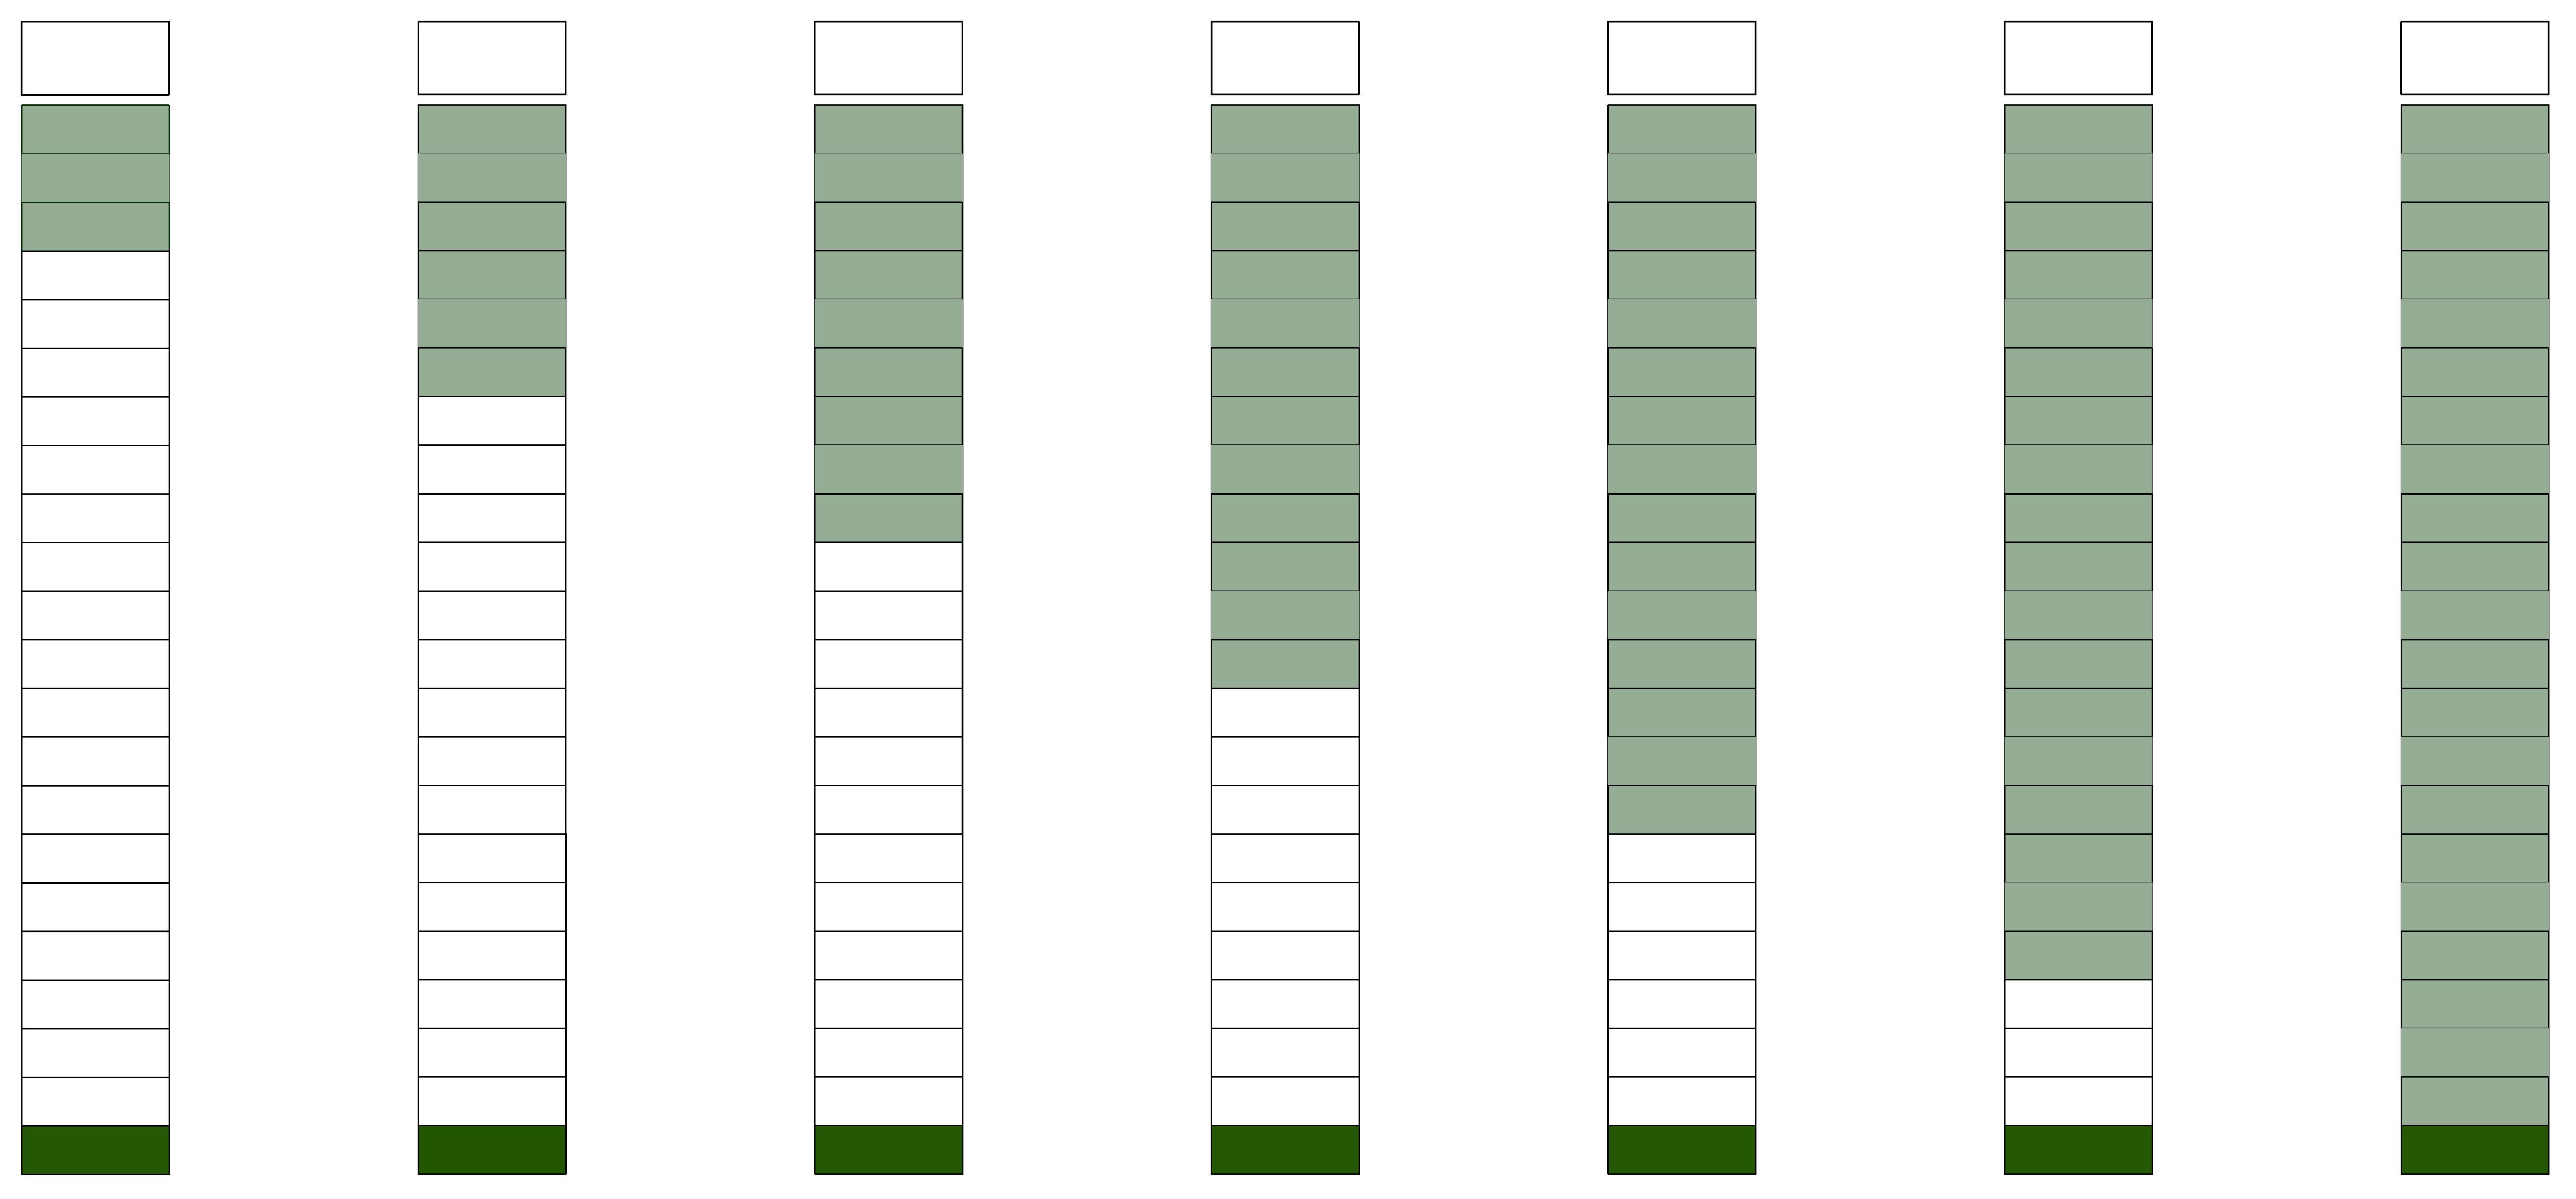
\includegraphics[width=0.9\columnwidth]{masse.pdf}
	\caption{\footnotesize{\textbf{Répartition de la masse dans un vorespace.} Le vorespace peut être vu, selon la masse, comme composé de 3 parties: 1 de 20 états correspondant à l'état d'équilibre (première case blanche), suivi de 21 cases représentant chaque paire gravité-charge et enfin l'état de blocage, en vert foncé. La fractalité exige que la répartition se fasse en 7 sauts, donc par saut de 3 doubles paires (en vert clair)}}
\end{figure}

À noter que ce modèle de distribution de masse est très hamiltonien.
Si $\omega$ est l'énergie du système, ce qui est le cas, alors les 128 états
possibles de la masse représentent l'espace de phase de sa distribution.
C'est un espace de Hilbert de dimension 7 ($2⁷=128$) et les $\omega$ sont les
états propres du système.

Cependant, avoir autant de masses pose un problème de simplicité
dans notre modèle de la plénodynamique quantique. Toujours en raison
du principe du rasoir d'Ockham, on stipulera qu'il n'y a qu'un seul type de masse
pour construire le modèle standard de la physique et on choisira la
plus lourde, $\omega_m$. On justifiera cette hypothèse dans le modèle
cosmologique du Big Bang.

On développera les conséquences d'un tel modèle de masse dans la
partie sur la gravité.

\subsection{La charge électrique}

Autant la masse est une aberration topologique du plenum, et donc de sa
physique, autant la charge électrique fait partie de sa nature. Il
est donc logique de gérer cette charge avec la seule physique du
plenum.

On définit la charge électrique $q_v$ du vorespace comme l'état stable de la
turbine, soit l'état des positions 1 à 20. En quelque sorte, la charge
électrique est son flux maximum (ou son flux nominal). Le flux
diminuant jusqu'à l'état 64, la charge diminue aussi. Elle s'annule au
«centre», puis s'inverse. Le signe change et la charge croit
négativement (ou positivement, si l'on part d'une charge négative).
Elle atteindra sa charge complète $-q_v$ dans les états 108 à 128.

Contrairement au cas de la masse, le cas de la charge électrique n'est
donc pas bloqué au moment de l'annulation de la charge. La physique du
plenum n'interdit en rien à la charge d'exploiter toutes les capacités
du vorespace.
\vspace*{-0.5cm}
\begin{center}
	\begin{longtblr}[
		%theme=widecaption 
		caption={\footnotesize{\textbf{Charge du vorespace}}},
		%label = {tblr:4-2},
		]{
			colspec={Q[c,m] Q[1.5cm,c,m] Q[, c,m] Q[2cm,c,m] Q[1.9cm,c,m]},
			rowspec={Q[m]},
			row{odd}={bg=blue!10!white},
			row{1}={c,mode=text,fg=white,bg=pkcolor, cmd=\textbf}, %cmd=\textbf, blue!80!orange
			rowsep=2pt, colsep=3pt,
			vline{2-Y} = {1}{0.3pt,gray!50},
			vline{2-Y} = {2-Z}{0.3pt,gray!30},
			hline{Z} = {0.1pt,blue},
			% nombre de col début et fin qui apparaissent à chaque page
			% 1 pour le titre par exempel
			rowhead = 1, %rowfoot = 1, 
		}
		États   & Nombre d'états &  Charge  &  Évolution de la charge &  Sens de rotation     \\
		1-19    &   20       &  $+q_v$  &       stationnaire      &      chiral           \\
		20-61   &   42       &  $+q_v$  &       baisse            &      chiral           \\
		62-65   &    4       &    0     &     stationnaire        &       aucun           \\
		66-107  &   42       &  $-q_v$  &       augmente          &      anti-chiral      \\
		108-127 &   20       &  $-q_v$  &       stationnaire      &      anti-chiral      \\

	\end{longtblr}
\end{center}



Comme toute la physique du plenum est gérée par une loi fractale à 7 pas, la charge
électrique n'échappe pas à la règle. Les nœuds stables étant les
charges stationnaires, il faut diviser la progression sur les 90 états
intermédiaires. D'autre part, pour les mêmes raisons qu'évoquées dans
le cas de la masse, ces états vont par paire. Mais cette fois-ci, la
physique de la charge concerne uniquement l'inclinaison de la pale.
Comme incliner la pale conduit aussi à adapter sa forme, et donc la
variation de charge, la variation d'inclinaison va de pair avec la
modification de la forme des pales. La double paire 62-65 étant
stationnaire, donc un état stable, elle ne compte pas dans les
états de transition. On a donc 84 états de transition, soit 42 paires
possibles. Avec une fractalité de 7, \textit{la charge varie par groupe de 6
paires.}

Il y a deux conséquences immédiates. La première est que la charge
varie par tiers. Elle passe de $q_v$, à \Ru{+}{2}{3}{e} et à \Ru{+}{1}{3}{e} avant de
s'annuler, puis de reprendre une progression inverse. Enfin, la
progression de la «variété électrique» est deux fois plus rapide que
celle de la masse. Voilà un début d'explication de la domination de la
force électrique sur la force de gravité.

On va désormais pouvoir étudier ces forces plus en détail.


\subsection{Les forces électriques et de gravité}

\subsubsection{Introduction}

Le modèle du plenum fabriqué précédemment souffre d'un grave défaut.
Il est statique. Comment construire les particules élémentaires du
modèle standard sans dynamique? C'est impossible! Il faut donc
trouver un moyen de créer cette dynamique. Nous allons établir qu'elle
vient (en partie) des forces électriques et de gravité. À cette fin,
nous allons nous pencher sur ces forces, même si, on le
verra, il sera nécessaire de postuler l'existence d'une particule
chargée pour terminer la démonstration des forces électriques. La
dynamique, responsable de la naissance des particules élémentaires du
modèle standard, va donc s'initier grâce à la gravité, puis se
consolider par l'effet cumulé de l'électrodynamique. C'est un modèle
très cosmologique, mais la plénodynamique quantique ne
prétend pas réinventer la physique! On verra toutefois dans le modèle
cosmologique du Big Bang que les masses possèdent aussi une vitesse de
dispersion énergétique initiale, à cause de la détente du «trou
noir» initial.

Bien que l'on pourrait ici s'intéresser uniquement à la gravité, comme
élément déclencheur, le fait que les forces électriques et de gravité
soient liées donne du sens à les aborder de concert. On mettra en
évidence l'existence de monopoles magnétiques et leur rôle dans la
gravité, en raccordant les visions de Paul Dirac et de Georges Lochak.
On établira aussi que le potentiel vecteur de l'électromagnétisme est
un véritable champ physique et, surtout, qu'il y en deux: les phonons de
gravité et ceux de charge. À partir de là, la plénodynamique quantique fera
sa première prédiction: la charge ralentit le temps, comme la masse
le fait aussi. On en déduira enfin une explication des effets
Aharonov-Bohm et Aharonov-Casher, qui seront les deux premières
preuves expérimentales de la véracité du modèle de la plénodynamique
quantique.

\subsubsection{La force électrique}

Le mécanisme de base de la force électrique est assez simple. Le
vorespace est chiral et possède un pas de vis. L'interaction entre
deux vorespaces voisins se fait structurellement via ce pas de vis. La
vision simpliste est celle d'un engrenage : si l'un tourne dans un
sens (chiral), le suivant tourne obligatoirement dans l'autre
(anti-chiral).

C'est la base. Deux vorespaces de chiralité opposée sont
structurellement liés (c'est la force d'attraction de particules de
même signe), tandis que deux vorespaces de même chiralité ne peuvent
se rencontrer sans bloquer leur rotation et rompre le plenum.
\textit{La force électrique est donc consubstantielle au plenum}. Elle lui
assure non seulement sa neutralité électrique, mais aussi sa forme.
Si le plenum est statique d'un point de vue de la structure, il est
dynamique d'un point de vue de l'énergie. On peut le voir comme un
échange permanent de flux d'un vorespace à l'autre. Par analogie avec
la mécanique des fluides, le vorespace agit comme une turbine pour le
fluide de l'information. Le mouvement du fluide est un pur
vortex, un tourbillon. Pour circuler, le fluide s'appuie sur la pale 
qui, en retour, s'équilibre par effet gyroscopique. Cet effet a toutes
les caractéristiques du champ magnétique. Il est perpendiculaire à la
pale, en sens opposé de l'appui du fluide. Il respecte bien la règle
des trois doigts par rapport au mouvement du fluide. Comme il existe
dans chaque vorespace sans boucler, c'est un monopole.

Le monopole magnétique n'est donc pas \textit{stricto sensu} une particule\footnote{On modulera plus loin cette affirmation en montrant qu'il existe réellement une particule ayant la propriété de monopole magnétique},
mais le couple de rappel d'un vorespace par réaction au passage du
flux. L'existence du monopole a été prédite par Paul Dirac en 1931 \cite{dirac1931quantised}.
Dans le cas du vorespace du plenum, étant donné l'alternance des vorespaces, les monopoles magnétiques s'annulent deux à deux. En conséquence, le magnétisme du plenum est nul.
En revanche, dès que l'on sort du cas nominal du plenum, par
adjonction de masse ou en touchant aux 88 positions potentielles, il est possible de faire apparaître
un monopole non nul.

On ne peut rien extraire d'autre du modèle statique du plenum.
Pour avancer, postulons l'existence d'une particule chargée
dans le plenum en anticipant son élaboration dans le chapitre suivant.
Quoi qu'il en soit, son existence est plausible, car elle existe dans
les particules élémentaires du modèle standard de la physique.
La chiralité de la particule n'est pas neutre par rapport au plenum.
Si on concentre en un endroit compact une super-chiralité, il se
produit une rupture de continuité du plenum autour de la particule.
C'est structurellement impossible : le plenum est un cristal rigide.
Si une rupture se présente, il se crée un vide, un vrai vide, une
absence de vorespace. Le plenum doit donc s'adapter.

La charge est directement reliée à l'angle de la rotation de la vis
(en réalité, sa double inclinaison possible). À la frontière entre la
particule massive et le plenum, les vorespaces n'ont pas d'autre choix
que de se «tordre» afin de faire riper l'engrenage. Se tordre veut
dire adapter l'angle d'engrenage. Tous les vorespaces périphériques à
la particule sont concernés. Bien entendu, il est impossible
d'encaisser sur une seule rangée la rupture d'équilibre provoquée par
la particule chargée. De proche en proche, chaque rangée de vorespaces
se tord afin d'étaler l'angle de rattrapage jusqu'à l'angle nominal du
vorespace. Visuellement, au niveau des pales turbines, il se créé un
\textit{cisaillement} à partir de la particule chargée.

Ce phénomène décrit une onde stationnaire. La particule chargée agit
comme une onde stationnaire sur le plenum afin d'assurer la continuité
du plenum pour ne pas le rompre. La forme de l'onde dépend bien
entendu de la forme de la particule, mais surtout de la manière dont
elle se transmet. Le milieu étant fractal, elle ne peut se transmettre
que par pas, selon un rythme de 7 pas avant de reboucler. L'onde est donc une rosace heptagonale
ouverte, à la manière de ce que l'on peut observer sur les photos des
novas quand elles aspirent les galaxies. L'analogie n'est pas
forcément fortuite: si l'univers suit une loi fractale, il est
normal de retrouver les mêmes images à toutes les échelles$\ldots$

On a donc crée un gradient structurel portant sur l'angle des doubles
hélices. Techniquement, l'onde varie aussi au cœur du vorespace, à
cause de la double hélicité, mais d'un point de vue macroscopique,
l'affirmation du gradient reste juste. C'est une onde de cisaillement.
En physique des solides, cette onde porte le nom de phonon. Comme le
plenum est un cristal, par analogie, on appellera \textit{phonon de
charge} cette onde de compensation de tension statique de la charge électrique.

Une conséquence immédiate est que la perturbation de l'angle
(ouvert ou fermé), sans changer la valeur de la rotation du vorespace,
induit une baisse de rendement du vorespace. En effet, le vorespace
doit «puiser» dans une des 108 positions potentielles pour s'adapter. Il
n'est plus dans sa forme nominale. La durée de transfert d'exergie
doit donc augmenter.

\textbf{Le temps ralentit donc à proximité d'une charge électrique!}

Il est clair que ce phénomène ne sera pas facile à observer à notre
échelle, car l'accumulation de charges nécessaires risque d'être
perturbée par un effet de claquage$\dots$

\subsubsection*{Comment expliquer la force électrique?}

C'est un effet purement exergétique, car la force électrique concerne
la chiralité, qui est intrinsèque au plenum. La force va donc être
gérée par la physique du plenum, qui est la thermodynamique.

Chaque particule chargée crée un phonon de charge qui est une onde
stationnaire heptagonale. Quand deux particules se rapprochent, les
ondes interfèrent. Quand deux particules ont la même charge, les ondes
s'additionnent et les vorespaces augmentent leur énergie de structure
(somme des énergies de chaque phonon). Le temps de traversée augmente, car la traversée est de plus en plus coûteuse. Les particules vont
privilégier les chemins énergétiques les plus bas (le talweg), qui
sont opposés. Elles vont reculer l'une devant l'autre. \textit{A contrario},
les particules de charges différentes s'attirent en minimisant
l'énergie sur le chemin de rencontre.

\subsubsection*{Qu'est-ce que le champ électrique?}

\textit{Le champ électrique est le gradient du phonon}. C'est donc la pente de
l'onde de cisaillement (qui est continûment ascendante ou descendante
à l'échelle macroscopique, en passant par une adaptation au sein des
deux hélices de chaque vorespace).

Comme le plenum est un cristal, on peut appliquer la loi de Hooke qui
stipule que, pour un cristal en cisaillement, le coût exergétique du
transfert est proportionnel au carré de la déformation de la maille.
En mécanique classique, on trouve que l'énergie du champ est
proportionnelle à $E^2$. Dans le plenum, la correspondance est que
l'exergie consommée est proportionnelle au carré de l'amplitude de
l'onde stationnaire de torsion.

\subsubsection*{Qu'est-ce que le champ magnétique?}

Le monopole magnétique seul ne permet pas d'induire ce qu'est le champ
magnétique. L'unique solution est de trouver une forme qui permette le
bouclage du champ sur lui-même, comme il est attendu. Sa construction
sort du cadre de cette partie. Par anticipation, on peut dire qu'un
candidat existe: c'est le hopfion.

\begingroup
\enlargethispage{0.38cm}
\endgroup
\begin{figure}[H]
	%\captionsetup{width=5cm}
	\centering
	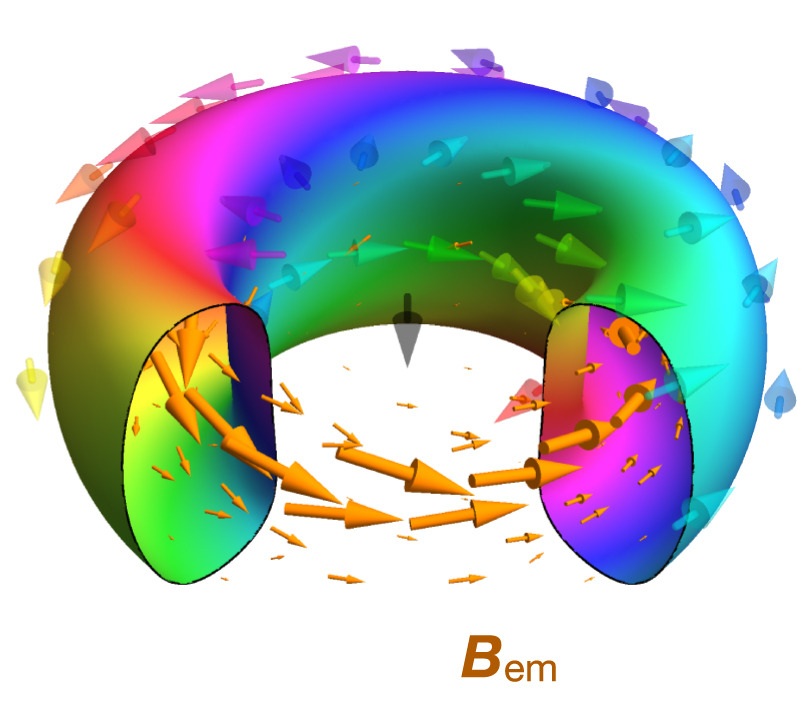
\includegraphics[width=0.9\columnwidth]{Hopfion.png}
	\caption{\footnotesize{\textbf{Le hopfion.} C'est le premier nœud stable du plenum qui agit en tant que dipole magnétique. On verra plus loin qu'il ressemble à un nœud $S_1$ ou $S_4$. (crédit: Wikipédia)}}
	\label{figure:1-hopfion}
\end{figure}


On note que le champ $\vec B$ étant toujours perpendiculaire à la pale et
que le phonon de charge créant une «continuité de pente de pales» dans
le plenum, le champ $\vec B$ résultant est bien perpendiculaire à cette
«onde de pales», conformément à ce que décrivent les lois de
l'électromagnétisme.

\subsubsection{La force de gravité}

Contrairement à la force électrique qui nécessite pour l'étudier de postuler
l'existence d'une particule chargée, il est possible de
créer un vorespace massique (ce qui n'a rien d'évident à prouver \textit{in
se}. On peut le postuler virtuellement pour cette partie, mais il
faudra prouver son existence par la suite. Heureusement, le modèle du
Big Bang permet de créer ces particules$\dots$) Toutefois, ce n'est pas
sans conséquence. On a vu que la masse déforme la turbine et forme
un bouchon topologique. Le plenum doit assurer la continuité autour de
la masse, pour ne pas se déchirer.

De même que l'angle varie pour la charge électrique, c'est désormais
la forme de la pale qui va s'adapter pour assurer cette continuité.
Bien que le résultat soit sensiblement identique dans la forme à celui
du phonon de charge, la dynamique qui prévaut est radicalement
différente. C'est la contrainte des pales qui donne un résultat
identique, mais la dynamique repose sur la forme dans le couple
inclinaison-forme. De même, pour la charge électrique, la dynamique
porte sur l'inclinaison. À l'instar de ce qu'il se passe pour la charge
électrique, il va se créer un \textit{phonon de masse} pour assurer la
continuité du plenum en présence d'une masse.

On aurait pu postuler que la masse cède de la vitesse aux vorespaces
aux alentours pour assurer cet équilibre. Cela aurait voulu dire que la masse
crée de la masse autour d'elle, en cédant de sa propre masse. Le
phénomène n'ayant jamais été observé, il n'a pas été retenu.
La masse crée donc un phonon de masse, c'est-à-dire une onde de masse.
C'est aussi une onde stationnaire, heptagonale. Le gradient est
l'expression du champ gravitationnel.

Attention, le gradient agit à la fois sur la crête des 7 onde,
mais aussi entre les 7 crêtes d'onde, via un double gradient$\ldots$ Il se
crée donc des talwegs d'onde masse.

On a par ailleurs vu que la physique de la masse sur le plenum n'est
plus la thermodynamique, mais la physique des flux. À noter alors le lien
profond qui apparaît avec le monopole magnétique. En effet, le
monopole magnétique est l'effet gyroscopique, la contre-réaction de la
pale au passage du flux. Si cet effet est nul dans le plenum, le
phonon de masse transforme la forme de la pale pour créer justement un
frein au flux. La gravité et le monopole magnétique sont donc
intrinsèquement liés. Cette idée rejoint celle de Georges Lochak sur
la nécessité d'avoir une masse pour le monopole magnétique \cite{lochak2002monopole}. On verra
d'ailleurs dans le modèle standard qu'il est possible de créer une
particule répondant aux critères d'un monopole magnétique et
que cette particule sera un neutrino, comme le
subodorait Georges Lochak \cite{lochak2002monopole}.

Bien entendu, comme le flux autour de la masse est perturbé par le
phonon de masse, le débit d'information n'est plus optimal,
c'est-à-dire analogue à celui du vorespace du plenum. Le temps de
traversée augmente.
\medskip

\textbf{En présence d'une masse, le temps ralentit.}

\subsubsection*{Qu'est-ce que la force de gravité?}

Analysons ce qu'il se passe quand deux masses sont proches l'une de
l'autre. On est désormais dans une physique du flux. Il y a deux cas
de figure, mais qui ont des résultats analogues quant à leurs effets.
Rien n'interdit à ce stade de la réflexion l'existence d'une masse
chirale ou antichirale. Techniquement, cela revient à avoir
une masse qui visse dans le plenum (sur un plan, on formerait une
cloche, à l'image d'une boule sur un drap) ou qui dévisse (toujours
dans un plan, l'image serait une boule qui pousse sous le drap, de
façon verticale).

En vis-à-vis des deux masses, leur phonon de masse respectif
interfère. Le flux, déjà réduit, diminue encore. Il se crée un
déséquilibre de flux entre les masses et autour des
masses. En hydraulique, un gradient de flux entraîne l'objet vers le
flux le plus tranquille. C'est le talweg du flux. Chaque masse se
dirige donc l'une vers l'autre, «roulant dans le talweg». \textit{C'est la
force de gravité.}

Il faut noter ici que la gravité respecte la thermodynamique. Si le
flux diminue, l'exergie baisse. D'un point de vue énergétique pure, les deux
masses se dirigent vers un minimum d'énergie, un talweg d'énergie.
Pour faire baisser l'exergie sans changer la vitesse de rotation du
vorespace, il faut aller puiser dans les réserves des 88 positions
possibles. C'est une augmentation d'entropie. Le talweg est
littéralement une dépression de néguentropie, la ligne de plus grande
pente vers l'état le plus «probable». Louis de Broglie l'avait
illustrée par cette image de talweg: «la trajectoire naturelle suit
le talweg d'une vallée de néguentropie.» \cite{debroglie1964thermodynamique}

Il faut ici bien comprendre ce qu'il se passe quand deux masses chirales et
anti-chirales se rejoignent. Les masses sont alors en opposition de phase.
L'une tire vers le haut, l'autre vers le bas. Leur rencontre est un
retour à l'équilibre. Techniquement, il y a une rupture de symétrie.
L'entropie extraite du plenum lui est restituée et elle est de nouveau
stockée potentiellement. Le plenum est à nouveau à l'équilibre (à
condition bien sûr que les masses chirales et anti-chirales aient la
même masse, sinon la différence forme une nouvelle masse, d'entropie de la
différence d'entropie des deux précédentes masses). On verra par la
suite que, de toute façon, ce cas n'est pas très intéressant, car
c'est juste une aberration créée dans nos accélérateurs de particules.
Le cas de deux masses de même chiralité est beaucoup plus intéressant.
D'un point de vue hydrodynamique, il n'y a aucune raison que deux
masses ne se rencontrent pas. Bien entendu, elles ne peuvent pas se
superposer, car il n'est pas possible de recouvrir deux vorespaces :
la rigidité du plenum l'interdit. En revanche, la dynamique de fusion
de la loi fractale qui régit le plenum autorise (et encourage) la 
fusion de deux masses. Deux masses ne se superposent donc pas:
elles fusionnent en une masse unique, en respectant au passage
l'échelle spatiale de la fractalité.

La gravité est donc le moteur de la fusion de notre modèle fractal.
Bien entendu, on sent bien que, si la rencontre entre deux masses est
indispensable, le plenum, en raison de l'intensité des flux au moment
de la rencontre, va subir une tension considérable, tension qu'il
faudra bien transformer en quelque chose. Ce quelque chose sera le
photon et on l'étudiera comme première particule du modèle standard,
même si \textit{stricto sensu} elle en n'est plutôt qu'un déchet de parcours.

\subsubsection{ Quelques conséquences}

\paragraph{Le potentiel vecteur}~\\ 

Les phonons de masse et de charge, s'ils sont extrêmement semblables
dans leur apparence, sont radicalement différents dans leur principe
créateur. Le phonon de charge est une onde de cisaillement et le
phonon de masse est une onde de flux. De leurs gradients respectifs,
on peut extraire une grandeur physique connue, la constante de
gravitation et le champ électrique.

Comme toujours en plénodynamique quantique, ces champs sont donc de
véritables champs physiques. On peut relier évidemment le phonon de
charge au potentiel vecteur du magnétisme, issu du rotationnel du
champ magnétique. Le magnétisme postule un champ de vecteurs purement
mathématiques. Ce champ est assurément le phonon de charge. Il existe donc bien
réellement. Comme on a vu que le magnétisme et la gravité sont
intimement liés, le champ de masse est aussi un potentiel vecteur
matérialisé. Ce sont les deux facettes d'un même champ, utilisées
différemment. C'est la raison pour laquelle la plénodynamique
quantique les différencie.

De même, le potentiel quantique de David Bohm \cite{bohm1952suggested}, dans sa théorie de
l'onde-pilote de de Broglie, est directement le phonon qui guide la
particule. On développera ce point quand on établira la compatibilité
entre la plénodynamique quantique et la mécanique quantique.

\paragraph{L'effet Casimir}~\\

Une application directe et intuitive des phonons est l'effet Casimir.
En mettant deux plaques en vis-à-vis qui sont bombardées en énergie sur
leur face opposée, il se crée une force qui aspire les plaques l'une
contre l'autre.

En bombardant chaque face, on augmente la valeur d'énergie au niveau
des plaques. Pour assurer une continuité du plenum, il se crée un
phonon de masse. L'interface des phonons entre les plaques crée une
baisse de flux qui crée une dépression, et donc l'attraction des deux
plaques.

\begin{mybox}[breakable,colback=blue!10, colbacktitle=pkcolor]{La force de gravité}
	La force d'attraction est donc un effet Casimir généralisé entre deux
	masses.
\end{mybox}
\medskip


\paragraph{Les effets Aharonov-Bohm et Aharonov-Casher}~\\


Si la mécanique quantique arrive encore à expliquer l'effet Casimir en
mobilisant l'«énergie du vide», ce qui est une façon de voir la
mobilisation de la réserve entropique du plenum qu'est le phonon, elle
n'explique pas les effets Aharonov-Bohm et Aharonov-Casher.

Quand on fait passer un électron entre deux fentes, il se forme
classiquement une figure d'interférence sur un plan de projection, si
les dimensions des fentes sont de l'ordre de la longueur d'onde de
l'électron. En revanche, placer un solénoïde chargé à proximité du
passage de l'électron perturbe la figure d'interférence, faisant
apparaître un retard de phase.

Le champ magnétique $\vec B$ n'étant présent --~selon les lois de l'électromagnétisme~-- qu'à l'intérieur du solénoïde, comment un électron
«sent-il» la présence du champ, alors qu'il passe à l'extérieur du solénoïde? La
physique actuelle ne l'explique pas.

En réalité, la frontière au niveau du solénoïde ne peut être brutale
au niveau du plenum. Il se crée un phonon de charge à l'extérieur.
L'électron traverse ce phonon, qui n'est plus un plenum équilibré. Le
temps de traversée augmente. La phase se décale.

Une preuve expérimentale de l'existence ce phonon serait de reculer le solénoïde.
Il existe une distance à laquelle le phonon de charge s'équilibre avec
le plenum. L'électron ne serait alors plus déphasé. Une expérience
avec une série de distances croissantes doit mettre en évidence un
retard de phases décroissant.

De même, la physique classique n'explique pas l'effet Aharonov-Casher.
Il s'agit cette fois de faire circuler une particule ayant un moment
magnétique, comme un neutron par exemple, le long d'une ligne
chargée. Il se crée cette fois un décalage de l'angle du spin. En
l'absence de champ magnétique, ce phénomène est inexplicable. La
présence d'un phonon de charge, en raison de la ligne électrique,
explique la présence du champ perturbateur. De même, on doit pouvoir
mettre en évidence la distance de coupure du champ via un protocole
similaire au précédent.

\subsubsection{Conclusions}

La force électrique, consubstantielle au plenum, est
régie par la thermodynamique. La force de gravité, contre-naturelle
au plenum, est régie par une physique différente de la physique
d'équilibre du plenum. C'est une physique des flux. Ces deux forces
font apparaître, chacune à leur manière, une torsion du plenum pour
assurer sa continuité sans le rompre. Comme le plenum est un cristal,
ce sont deux phonons, de charge et de masse. En réalité, les deux
phonons sont liés : la torsion est le moteur de l'un et la gestion du
flux le moteur de l'autre. Ce sont les deux faces d'une même pièce,
selon la façon dont elles sont employées. Le gradient des phonons donne
alors les valeurs des champs électrique et gravitationnel. On note
que le champ gravitationnel et le champ magnétique sont liés par le
même mécanisme. Enfin, le monopole magnétique existe, comme effet
gyroscopique des pales du vorespace au passage du flux entropique. Il s'annule
à l'équilibre et se révèle bien entendu quand l'entropie
augmente.


\section{Le modèle standard de la physique}

\subsection{Introduction}

Pour le moment, le modèle proposé est satisfaisant, car il est
compatible avec l'électromagnétisme et la gravité. Il explique de
plus les effets Aharonov-Bohm et Aharonov-Casher, ce qui n'est pas
rien. Il doit désormais expliquer la création des particules
élémentaires du modèle standard pour être validé.

Il faut au préalable mettre au jour la véritable nature du photon. En effet, jusqu'à présent, la
physique ne faisait que constater l'existence du photon et en prendre
acte. Nous allons répondre à la grande question que se posait Albert
Einstein: «Si seulement on pouvait comprendre $E=h\nu$!»\cite{einstein1994correspondence} On va
découvrir que le photon est hors-modèle, car il est, à l'instar de la
force de gravité, une anomalie du plenum. Mais au lieu d'être une
anomalie utilisant du potentiel du vide, il est une anomalie de
structure, de dimension.

\subsection{Le photon}

\subsubsection{Le modèle du photon}

Le problème consiste à construire un photon à partir de vorespaces du plenum, qu'ils
soient massiques ou non. Ce sont en effet les seuls «outils» à notre
disposition et nous ne pouvons pas faire autrement que de
utiliser.

La difficulté est de créer une particule de spin 1 à partir de
particules de spin \R{1}{2}. La solution évidente est d'assembler deux
particules de spin \R{1}{2}. Dans le plenum, deux vorespaces consécutifs
sont alternés, pour assurer une neutralité électrique, mais aussi la
nullité du spin. Il faut donc retourner un vorespace pour en mettre
deux en vis-à-vis. La tête de vis de l'un fait donc face à la pointe
de vis de l'autre. La somme des spins fait bien 1: le
«double-vorespace» est un boson. L'image d'un photon composé de deux
demi-photons de Louis de Broglie prend corps. \cite{debroglie1934une}

Deux problèmes surgissent instantanément. Il est impossible de
retourner un vorespace dans le plenum sans déchirer le plenum lui-même, car il est rigide.
Techniquement, il est donc impossible de créer un photon par la loi
fractale du plenum.

Supposons toutefois que cela soit possible. Ce double-vorespace est en
réalité un couple (vorespace, anti-vorespace). Les deux vorespaces sont
en tout point identiques, mais de façon miroir. Ils doivent
s'annihiler. Quel est donc ce processus, d'où vient-il et que
produit-il au final?

La création d'un photon dans le plenum est \textit{a priori} une impossibilité
structurelle. Le photon est techniquement une aberration topologique,
et son processus d'élaboration est contraire aux lois du plenum.
Heureusement, la gravité vient sauver le photon.

Revenons à l'instant où deux masses se rapprochent pour fusionner. Leurs
phonons de masse s'additionnent, créant sur le chemin des
vorespaces hyper-entropiques. Leur vitesse est toujours $\omega_v$, mais
l'onde de cisaillement écrase littéralement la turbine en
l'aplatissant: il arrive un moment où la turbine devient un
«disque» , obstruant tout le passage. Le flux est alors coupé.
L'approche des masses étant symétrique, on est assuré qu'au moins deux
vorespaces voisins ont atteint cet état.

La pression sur les vorespaces devient gigantesque, puisque d'un côté
le flux est nul et que, de l'autre, il est très grand. Tout est
bloqué. Cependant, la masse a une vitesse qui excède la vitesse de
rotation du plenum bloqué. Elle peut donc encore forcer en cédant une
partie de son énergie excédentaire. Le coup de vis supplémentaire
vient donc à bout de la résistance du plenum, qui «craque». Pour
faire craquer le plenum, la masse doit donc céder une énergie
correspondant à la masse du vorespace, soit $\omega_v$.

Visuellement, les deux vorespaces, qui sont des disques, entrent
l'un dans l'autre. La pénétration se fait au détriment de la surface.
En 7 pas, elle s'arrache complètement. Au 8\ieme\ pas, les deux sphères
deviennent deux disques entrelacés.

Concrètement, les vorespaces ont perdu leur surface, qui venait du 3\ieme\
degré de liberté. Les deux cercles sont donc un vorespace à deux
degrés de liberté. On pourrait alors s'amuser à élaborer plein de
théories pour trouver à quoi ressemble ce nouvel assemblage, mais cela
a déjà été fait. C'est toujours un bi-vecteur de Clifford, mais à deux
degrés de dimension, une v-sphère $S_2$. Elle est composée de deux
cercles perpendiculaires qui ont une rotation liée, permise autour
d'un axe qui les relie en les «soudant» autour de deux points fixes.

La meilleure image que l'on puisse s'en faire est celle d'un cardan.

On remarque immédiatement que deux cercles en rotation liée forment un
photon. La gravité, en pliant le plenum, a donc créé un photon.

Le processus n'est pas terminé. Les masses continuent leur poussée sur
le photon qui se met en rotation. Il tourne évidement selon un
processus à 7 pas, donc par pas de $2\pi/7$. À chaque pas, les deux
cercles s'enroulent autour d'un vorespace voisin et, au septième, ils
se sont totalement enroulés. On remarque alors que le photon n'a fait
lui-même qu'un demi-tour. Rien ne freine le photon, car il n'entre pas
en interaction avec le vorespace. Il ne peut donc que continuer à
s'enrouler. À la fin du second vorespace, il finit sa propre rotation
complète. Il lui faut donc deux vorespaces pour effectuer une rotation
complète, confirmant l'intuition de de Broglie que le photon soit
composé de deux demi-photons. En réalité, sa dimensionnalité inférieure
l'oblige à s'adapter à son nouvel espace.

Rien n'arrête plus le photon qui s'enroule toujours selon les brins
d'ADN du plenum. Il circule donc à la vitesse nominale de transmission
d'un vorespace, c'est-à-dire à c.

\subsubsection{Les conséquences}

Il y a énormément d'informations dans le processus précédent. Le photon est une
rupture de symétrie du plenum qui est un équilibre thermodynamique. En
tant qu'anomalie topologique, sa co-existence dans le plenum en tant
que particule statique est impossible: le photon ne fait pas partie de
l'univers du plenum. Sa dynamique est donc une réponse à cette
impossibilité: il est condamné à fuir, ne pouvant se fixer. Sans
masse, il circule comme un superfluide, à la vitesse maximale
autorisée par le plenum. Mais sa vitesse et sa masse sont aussi un
moyen de conserver la masse statique du plenum, sans quoi la
disparition de deux vorespaces changerait l'équilibre global du plenum.
L'énergie totale est  bien conservée. Chaque masse fusionnée a perdu
l'énergie d'un vorespace, donc diminué sa rotation de $\omega_v$.\footnote{On verra en réalité que le processus est dynamique et que le coût exergique est décomptée du mouvement.} L'énergie
totale du plenum n'a pas été modifiée.

Une conséquence est que la physique du photon est aussi différente de celle du plenum, 
qui est purement exergique, à l'instar de celle de la force
électrique. La force de gravité est quant à elle une physique du flux. La physique
du photon repose ainsi uniquement sur l'entropie. Le photon est en quelque sorte \textit{un
révélateur entropique}. Par son double-mécanisme d'emboîtement, de
l'ouverture du photon et de la rotation de la vis du vorespace, le
passage du photon est littéralement «collé» au vorespace et le suit
dans toutes ses fluctuations entropiques. 

En conséquence, le photon,
non seulement décode l'entropie du vorespace, mais se dirige toujours
vers les gradients positifs du phonon, c'est-à-dire en «surfant sur
la crête entropique» ou, comme l'avait dit Louis de Broglie, «en
suivant les talwegs de néguentropie». Dit autrement, c'est le
second principe de la thermodynamique qui est mis à jour, non pas
comme un principe sorti de l'expérience humaine, mais comme une
contrainte de vissage entre un photon et un vorespace. 

\begin{mybox}[breakable,colback=blue!10, colbacktitle=pkcolor]{Second principe de la thermodynamique}
	Le second principe de la thermodynamique est en réalité un mécanisme 
	structurel.
\end{mybox}
\medskip


De plus, la création du photon permet de finir d'élaborer la fusion de
masse fractale. Il est nécessaire qu'il y ait un nombre pair de
vorespaces entre les masses. Quand le groupe de paires ou la paire de
vorespaces atteint son entropie maximale, alors la gravité peut les
transformer en photons, pour finir d'ouvrir la voie. Quand il n'y a
plus de vorespace entre eux, les masses sont en contact. \textit{C'est la
fusion}. Il est probable que l'émission de photon suivent aussi une loi
de création par groupe de 7.

Enfin, le photon, en tant que sous-produit de la gravité, révèle en
miroir une structure sous-jacente du plenum. Si l'on peut briser la
symétrie des particules, on peut briser la symétrie de la structure
entière. \textit{On pressent alors que le plenum est le résultat d'une
structure précédente à deux dimensions via un passage fractal}. Le
photon est donc une résurgence du passé. On verra par la suite, grâce
au modèle du Big Bang, qu'il est en réalité comme un jeune conducteur qui
découvre l'ivresse de la vitesse. Quoi qu'il en soit, cela
«justifie» la répartition d'énergie supposée, en divisant par deux
dans la «fusion arrière». La loi fractale doit être respectée dans
le passage à l'échelle. On reviendra sur tout cela quand on abordera
le modèle du Big Bang.

\subsection{Le modèle des particules élémentaires du modèle standard}

Attaquons-nous désormais à la construction des particules élémentaires
du modèle standard de la physique. À cette fin, on postulera une
abondance de masses élémentaires de vitesse $\omega_m$. La processus de fusion
se fera via la gravité et suivra un processus fractal non
dimensionnellement restreint.

Pour rappel, la liste des particules élémentaires à créer est rappelée dans le tableau \ref{tblr:4-epe}.

\vspace*{-0.5cm}
\begin{center}
	\begin{longtblr}[
		%theme=widecaption 
		caption={\footnotesize{\textbf{Énergie des particules élémentaires}}},
		label = {tblr:4-epe},
		]{
			colspec={Q[c, co=1]  Q[c] Q[c, co=1] },
			rowspec={Q[m]},
			row{odd}={bg=blue!10!white},
			row{1}={c,mode=text,fg=white,bg=pkcolor, cmd=\textbf}, %cmd=\textbf, blue!80!orange
			rowsep=2pt, colsep=3pt,
			vline{2-Y} = {1}{0.3pt,gray!50},
			vline{2-Y} = {2-Z}{0.3pt,gray!30},
			hline{Z} = {0.1pt,blue},
			% nombre de col début et fin qui apparaissent à chaque page
			% 1 pour le titre par exempel
			rowhead = 1, %rowfoot = 1, 
		}
		Particules               &   Désignation         & Masse                    \\
		Photon                   &        $\gamma$       &  0                       \\
		Gluon                    &            g          &  0                       \\
		Neutrino électronique    &        $\nu_e$        &  < 0,8 $eV/c^2$          \\
		Neutrino muonique        &        $\nu_\mu$      &  < 0,17 $MeV/c^2$        \\
		Électron                 &           $e^-$       &  0,511  $MeV/c^2$        \\
		Quark up (u)             &            u          &  $\approx$ 2,2 $MeV/c^2$ \\
		Quark down (d)           &            d          &  $\approx$ 4,7 $MeV/c^2$ \\
		Neutrino tauique         &        $\nu_\tau$     &  < 18,2 $MeV/c^2$        \\
		Muon                     &        $\mu^-$        &  105,7 $MeV/c^2$         \\
		Quark strange (s)        &            s          &  $\approx$ 95 $MeV/c^2$  \\
		Quark charm (c)          &            c          &  $\approx$ 1,28 $GeV/c^2$\\
		Tau                      &         $\tau$        &  1,77 $GeV/c^2$          \\
		Quark bottom (b)         &            b          &  $\approx$ 4,18 $GeV/c^2$\\
		Boson W                  &         $W^\mp$       &  80,4 $GeV/c^2$          \\
		Boson Z                  &           $Z_0$       &  91,2 $GeV/c^2$          \\
		Boson de Higgs           &           $H_0$       &  125,1 $GeV/c^2$         \\
		Quark top (t)            &            t          & $\approx$ 173 $GeV/c^2$ \\
	\end{longtblr}
\end{center}


Il va donc falloir faire entrer cette liste dans un processus fractal.
Or il a été choisi initialement le processus fractal de l'algèbre de
Clifford, à savoir 7 nœuds possibles, les $S_1$ à $S_6$. Ces
nœuds vont donc être composés de vorespaces massiques, en progression
de la loi fractale.

On peut se les représenter et obtenir quelques informations
caractéristiques (\textit{cf.} tableau \ref{tblr:5-0-1}).
On voit donc clairement apparaître une composition naturelle de $S_1$ à
$S_6$, avec trois formes (cercle, double-cercle et hélice), avec une rupture
de composition pour la 7\ieme\ forme qui est une fin dans l'algèbre de
Clifford.

Postulons donc qu'à cette échelle, la fin du processus conduise à nos
premières particules physiques, les hadrons, à savoir le neutron et le
proton. Techniquement, le neutron et le proton seraient des nœuds $S_8$.

%\vspace*{-0.5cm}
\begin{table}[H]
	\centering
	\caption{\footnotesize{\textbf{Nœuds de l'algèbre de Clifford $S_{7,0}(\mathbb{R}$)}}}
	\label{tblr:5-0-1}
	\begin{tblr}[
		%theme=widecaption 
%		caption={\footnotesize{\textbf{Nœuds de l'algèbre de Clifford $S_{7,0}(\mathbb{R})$}}},
%		label = {tblr:5-0-1},
		note{$\dagger$} = {composée de vorespaces, donc c'est une suite ressemblant au brin	d'ADN, un tube continu variant d'un maximum à un minimum.},
		]{
			colspec={Q[c,m]  Q[2cm, c,m] Q[4cm,c,m] Q[c,m] },
			rowspec={Q[c,m]},
			row{odd}={bg=blue!10!white},
			row{1}={c,mode=text,fg=white,bg=pkcolor, cmd=\textbf}, %cmd=\textbf, blue!80!orange
			rowsep=2pt, colsep=3pt,
			vline{2-Y} = {1}{0.3pt,gray!50},
			vline{2-Y} = {2-Z}{0.3pt,gray!30},
			hline{Z} = {0.1pt,blue},
			% nombre de col début et fin qui apparaissent à chaque page
			% 1 pour le titre par exempel
			rowhead = 1, %rowfoot = 1, 
		}

		Nœud    & Quantité de vorespaces   &            Forme\TblrNote{$\dagger$}                   & Spin \\
		$S_1$   &         $2^8$            &        Cercle                                          &  0   \\
		$S_2$   &         $2^{16}$         &        2 cercles perpendiculaires                      &  1   \\
		$S_3$   &         $2^{24}$         &        Double hélices entremêlées                      & \R{1}{2}  \\
		$S_4$   &         $2^{32}$         &        Tore des doubles hélices précédentes            &  1   \\
		$S_5$   &         $2^{40}$         &        2 tores précédents perpendiculaires             &  1   \\
		$S_6$   &         $2^{48}$         &        Double hélices des tores précédents             & \R{1}{2}  \\
		$S_7$   &         $2^{56}$         &        7 doubles hélices précédentes emmêlés en hélice & \R{1}{2}  \\
	\end{tblr}

\end{table}

Ils doivent donc être composés de $2^{64}$ masses élémentaires, ce qui
revient à dire que leurs tailles sont proportionnelles à la taille de la
masse élémentaire, donc du vorespace :

\begin{equation*}
	L_{hadron}  = 2^{64} \cdot L_v
\end{equation*}


On a donc $L_v = L_{hadron}/2^{64}$

avec
\begin{equation*}
	\left\{
		\begin{split}
	 		L_{neutron} &= 0,8 \cdot 10^{-15}\,m  \\ 
	 		L_{proton}  &= 0,88 \cdot 10^{-15}\,m 
		\end{split}
	\right.
\end{equation*}

$L_v$ oscille donc entre $4,3 \cdot 10^{-34}\,m$ et $4,8 \cdot 10^{-34}\,m$, soit un peu plus
de 20 fois la longueur de Planck ($L_p=1,6 \cdot 10^{-35}\,m$). Sachant que c'est
une approximation de la longueur du hadron, ce résultat conforte
l'hypothèse hadronique comme résultat de la périodicité de Bott. On
pourrait donc avoir


\begin{equation*}
	L_v \approx 20 L_p
\end{equation*}

On ajustera cette longueur grâce aux propriétés du photon, dans la
partie réservée aux constantes de la physique.
\medskip

Tâchons de voir désormais comment ranger les particules élémentaires
dans les nœuds de l'algèbre de Clifford. On a déjà un problème
évident : il y a plus de particules élémentaires que de nœuds. De
plus, un nœud étant stable, il a donc une unique énergie et on ne peut
ranger deux particules de massses différentes dans le même nœud. On a
donc au moins 17 particules à essayer de faire entrer dans 7
nœuds.

Il y a un premier tri assez facile à faire. Il suffit de comparer les
valeurs de spins. Le gluon, avec sa masse nulle, ne peut entrer nulle
part. Les bosons Z et $W^\pm$, avec leur grande masse, correspondraient à
des particules très lourdes, donc des $S_6$ ou des $S_7$. Leur spin de 1
rend cette appartenance impossible. De même, les neutrinos ont des
masses très légères, donc devraient être des nœuds $S_1$ ou $S_2$ au
maximum. Leur spin de \R{1}{2} rend aussi impossible cette appartenance.
Les quarks, avec leurs charges fractionnaires, rendent problématique
un rattachement à un quelconque nœud: nulle part, dans la loi de
fractalité, la chiralité se divise. Il ne reste donc que l'électron,
le muon et le tau. Leurs spins les obligent à être au moins un nœud
$S_3$ et leurs énergies placeraient ces particules dans les nœuds
suivants:

\begin{center}
\begin{tabular}{ c c l }
	$S_3$ & $\rightarrow$ & électron \\
	$S_6$ & $\rightarrow$ & muon     \\
	$S_7$ & $\rightarrow$ & tau 
\end{tabular}
\end{center}

Examinons rapidement le cas $S_3$ pour l'électron. $S_3$ est un passage à
l'échelle du vorespace, donc si ce cas est avéré, cela veut dire que
les positions 1 à 19 de l'électron correspondent à la charge
élémentaire de l'électron, soit $q=-1,6\cdot10^{-19}\,C$. La charge est une
caractéristique interne du vorespace, elle est invariante par
changement d'échelle. On en déduit que la charge élémentaire du
vorespace est aussi q, donc $q_v=-e$. On retrouve bien que la charge est
un invariant relativiste.

C'est tout ce qu'il est possible de déduire à ce stade. On pourrait croire
que le modèle standard n'est pas compatible avec la loi fractale de la \PQ.

Est-ce la fin de la partie? Non, car jusqu'à présent, on a supposé
que le modèle engendrait ses nœuds sans interagir avec le plenum, ce
qui est clairement faux. On a vu qu'au niveau du plenum, quand deux
charges fusionnent, il se forme au moins un photon. Se pourrait-il
qu'il se produise d'autres particules?

Examinons les cas et appliquons résolument la loi fractale à partir de
la masse unitaire.

\subsubsection{Premier nœud: la première particule de l'univers}

Le premier nœud $S_1$ rassemble donc $2^8$ vorespaces massiques. Chaque
paire a engendré (au moins) un photon et, par conséquent, chaque
liaison s'est trouvée réduite de la masse d'un vorespace du plenum. Le
nœud forme un cercle de 256 vorespaces. C'est un élément extrêmement
léger qui aurait pu faire un candidat au rôle de neutrino, si son spin
de 0 avait été compatible.

Malheureusement, dans la description précédente de la fusion de deux
vorespaces massiques, il n'a pas été tenu compte de leur vitesse de
rotation. Quand deux vorespaces massiques s'associent, ils ne peuvent
s'associer que tête-bêche, les parties hautes des turbines ensemble.
Cette association implique que les turbines tournent en sens
contraire. Si l'on associe deux turbines chirales, il faut trouver un
processus qui inverse la chiralité de l'une pendant le processus de
fusion. Cette opération est forcément asymétrique (l'une change de
chiralité, pendant que l'autre reste chirale) et exige un processus
compliqué. Il est bien plus simple, toujours selon le principe du rasoir d'Ockham,
de postuler l'existence d'un vorespace massif anti-chiral. Cette
hypothèse sera confirmé lors du modèle du Big Bang.

Dès lors, le processus évoqué précédemment reste pertinent, et même
favorisé, puisque deux vorespaces massifs anti-chiraux vont se
rapprocher plus facilement, comme lors d'une rencontre de deux
particules de charge opposée. Quoi qu'il en soit, on verra que dans le
modèle du Big Bang, les particules ont en plus une cinétique très
importante, qui prendra de toute façon le pas sur tout.
Les vorespaces du plenum subissent donc exactement le même processus,
à la différence près que deux vorespaces voisins se mettent chacun
dans l'état de disque, soit par un processus décroissant (44\ieme\
paire, position 62-63), soit par un processus croissant (66\ieme\ paire,
position 63-64). Techniquement, leur position respective, l'un placé «au-dessus» de
l'autre, favorise la rencontre, puis le déchirement et la perte
dimensionnelle qui s'ensuit. Le photon naît donc de la fusion d'un
vorespace massif et d'un vorespace anti-massif.

L'élément obtenu garde la chiralité du vorespace massif. S'il y autant
de vorespaces massifs qu'anti-massifs (hypothèse qui sera justifiée dans
le modèle du Big Bang), il se crée autant d'éléments chiraux
qu'anti-chiraux et le processus peut se répéter. À la 7\ieme\ étape, il
n'existe plus que deux types d'éléments : un élément chiral de 128
vorespaces et un élément anti-chiral de 128 éléments. Le nœud suivant
est celui de la stablitié, ce qui veut dire implicitement que tous les
éléments massifs (et donc anti-massifs) ont été consommés.
La première particule massive est donc un nœud $S_1$. Elle ressemble à
un tore d'ADN chiral, composé de 256\,~masses élémentaires, et donc de
périmètre $256 \cdot 2L_v$, soit $512 \cdot 1,616 \cdot 10^{-35} = 8,274 \cdot 10^{-33}\,m$. Son rayon
est donc $5,267 \cdot 10^{-33}\,m$.

On peut essayer d'imaginer le phonon de masse engendré par une telle
particule. La rotation du tore, par pas de $2\pi/7$, engendre une onde
heptagonale. La rotation interne des doubles-hélices ajoute une onde
heptagonale dans le sens des pales qui va favoriser le chevauchement
de deux particules de ce type.

\subsubsection{Nœud $S_2$: la seconde particule de l'univers}

En effet, l'étape suivante consiste à créer un nœud $S_2$ à partir de
deux nœuds $S_1$. On est toujours dans un processus forcé dynamiquement,
mais dès ce stade, la gravité peut suffire à expliquer complètement le
processus. Deux nœuds $S_2$ se rapprochent par gravitation pure. À cause
des phonons «perpendiculaires», ils ne peuvent fusionner dans le
plan de rapprochement, comme à l'étape 1. Les deux phonons les
obligent à se chevaucher, donc à passer l'un sur l'autre. Les deux
phonons «perpendiculaires» les placent donc là où le flux est 
moindre, c'est-à-dire perpendiculairement l'un à l'autre. La pression fait le
reste et les deux tores s'emboîtent en 7 fois $2\pi/7$\ieme\ de tour de tore
respectif. La chiralité est identique sur les deux tores et est donc
conservée à l'ensemble: le «primo-photon» de masse $S_2$ est né. À
noter qu'à l'interface des jonctions, les vorespaces du plenum sont
écrasés selon un processus identique à celui de l'étape 1: il se crée donc
encore des photons.

Bien entendu, le processus continue par fractalité. 2
«primo-photons» fusionnent, chaque tore perpendiculaire fusionnant
 selon un processus de double-enroulement. Le processus se
répète 7 fois, produisant son lot de véritables photons, jusqu'à
l'étape final du nœud $S_2$, à la huitième étape.

La seconde particule de l'univers ressemble donc à deux tores
(eux-mêmes composés de 7 tores enroulés) d'ADN imbriqués,
perpendiculaires l'un à l'autre, en rotation chirale, chaque tore
faisant un $2\pi/7$\ieme\ de tour à chaque fois. Il est composé de $2^{16}$
éléments de masse élémentaire. Le phonon de masse commence à être
difficile à décrire. Il s'agit en réalité d'un sous-ensemble de la
fibration de Hopf qui ne garde que 7 cercles de la fibration, chacun
étant bien entendu décalé de $2\pi/7$. Malgré tout, on ne peut imaginer
réellement qu'un seul phonon à la fois à chaque étape de la fibration, car imaginer leur
combinaison commence à faire mal à la tête$\ldots$ Quoi qu'il en soit, on
commence à se rapprocher d'un champ gravitationnel sphérique autour de
la particule, même s'il est $2\pi/7$-périodique.

\subsubsection{Le troisième nœud: et l'électron fut}

Il faut répéter ce processus pour le troisième nœud, avec un
processus fractal qui va aussi se développer dans la troisième
dimension, ce qui nous mènera mécaniquement à $2^{24}$ masses élémentaires
pour sa composition. L'idée générale sera de «dévisser» chaque tore,
en l'élevant dans une dimension verticale. Le dévissage se fera de
concert avec les deux tores perpendiculaires, entraînant un
emboîtement des déroulements, et donc, au final, une double-hélice. La
dimension grossissant aussi par pas de $2\pi/7$, la largeur de
l'enroulement sera plus grande à l'arrivée qu'au départ, d'où la forme
de turbine. Enfin, la rotation ne pourra être transmise qu'à l'une
des deux hélices, sinon le processus de déroulement ne serait pas
possible: en quelque sorte, l'une cède peu à peu sa rotation pour
permettre la rotation de l'ensemble dans la dimension supérieure.

On peut quand même essayer de décrire le processus de fusion. Deux
particules $S_2$ fusionnent. Il n'y plus de possibilité d'enrouler les
tores avec les 7 déjà enroulés, donc le tore est obligé de rester
extérieur à l'enroulement. Le processus se faisant par pas de $2\pi/7$,
il se crée un décalage spatial et angulaire de $2\pi/7$ entre les deux
tores. Il en va de même avec le tore perpendiculaire. L'équilibre de
rotation de l'ensemble est perturbé et pour que les deux $S_2$ restent
emboîtés, le tore perpendiculaire doit céder $2\pi/7$ de sa vitesse
angulaire. Le processus se répète 7 fois, jusqu'au premier nœud
primo-stable. Il s'est crée deux pas de vis emmêlés qui est le premier
pas de vis de la particule finale. Ces primo-nœuds rencontrent
d'autres primo-nœuds en fusionnant pour donner, à chaque fois, un pas
de plus, jusqu'au 7\ieme\ nœud, c'est-à-dire le nœud $S_3$.

On se retrouve à cette étape avec une copie conforme du vorespace massique, à
l'échelle, composée de $2^{24}$~éléments massiques. Sa
structure compatible avec la définition d'une charge électrique et son
spin de \R{1}{2} le rend compatible avec le rôle de l'électron. Sa masse
totale inclut toutes les énergies de fusion, parties en photon.

Si l'on accepte que le nœud $S_3$ est bien un électron, alors:

\begin{itemize}
	\item l'électron serait la première particule élémentaire connue de l'univers
	créée dans ce processus;
	\item le vorespace a bien une charge de $e=1,6 \cdot 10^{-19}\,C$.
\end{itemize}

On peut calculer la masse élémentaire fusionnée :
\begin{equation*}
m_{e^-_{fusion}} = \frac {0.511 \cdot 10^6} {2^{24}} = 3,05 \cdot 10^{-2}\,eV/c²
\end{equation*}

Bien entendu, il faut retirer les énergies de chaque
photon engendrées par la fusion, et donc connaître l'énergie de masse du
vorespace. Or on sait que $\omega_m = 2 w_v$ et que chaque vorespace a coûté
une fusion, donc on en déduit que
\begin{equation*}
m_{e^-} = \frac{1}{2} m_{e^-_{fusion}} = 1,52 \cdot 10^{-2}\,eV/c²
\end{equation*}

et, de fait, $m_{v_{massique}} = 0,75 \cdot 10^{-2}\,eV/c²$
\medskip

À noter que le champ gravitationnel devient extrêmement complexe. Il
s'agit encore d'une fibration à 7\,~pas, mais la triple imbrication des
rotations rend la visualisation du champ résultant extrêmement
difficile à concevoir.

\subsubsection{Le nœud 4 ou le combat des forces}

\paragraph{Le modèle de concurrence charge-gravité (CCG)}~\\

Jusqu'ici, la fusion est purement gravitationnelle. Mais à partir de
$S_3$, le nœud comporte une charge et il va falloir en tenir compte.
En effet, le nœud suivant, selon la logique de la loi fractale, doit
faire fusionner deux $S_3$, soit deux électrons ensemble, leur charge de même signe
rendant théoriquement le rapprochement impossible. Il est nécessaire
d'introduire une énergie permettant d'outrepasser cette
impossibilité. On admet pour la suite que les électrons sont dotés
d'une vitesse, et donc d'une énergie cinétique, rendant la rencontre
possible, comme dans un accélérateur de particules. On justifiera
cette hypothèse lors de l'étude du modèle cosmologique du Big Bang.

Effectuons une légère parenthèse et étudions ce qu'il se passe lors
d'une rencontre hypothétique de deux vorespaces purement chiraux, de
même chiralité. Entre les deux, sur le chemin de la rencontre, le
phonon de charge croît, par addition de leurs deux phonons respectifs.
En théorie, les déplacements sont contrariés, mais la cinétique
continue à les pousser l'un vers l'autre. Quand l'un des vorespaces
intermédiaires a exploité ses 42 premières positions, il n'a pas d'autre
choix que de continuer. Il atteint la zone de nullité. Le vorespace
perd donc sa charge, déséquilibrant l'équilibre électrique local du
plenum. La charge nulle crée un «trou», qui n'a pas d'incidence
locale. La pression continue et le vorespace va chercher à exploiter
les positions suivantes. Sa chiralité s'inverse : il change de signe,
jusqu'à se retrouver totalement symétrisé de sa position de départ. Il
se retrouve donc à l'envers (tête contre tête) et en rotation inverse
avec son voisin dans la même branche d'ADN. Il peut ainsi s'enrouler
avec lui, en ne formant qu'un seul vorespace. Il ne reste qu'un
cercle. Le spin n'ayant pas changé dans le retournement, il
s'additionne avec celui du voisin, identique. L'objet devient un
boson. Les chiralités s'annulent, ainsi que les enroulements. Il ne
reste qu'un cercle, qui se confond avec l'emboîtement du vorespace
suivant. Deux vorespaces ont disparu. Le «coût» énergétique s'est
forcément dilué dans la cinétique.

Bien entendu, ce cas n'existe pas dans la réalité, les particules
chargées étant forcément massiques. Il va donc falloir intégrer le
phonon de masse dans le processus.

La problématique va consister à mesurer la concurrence entre la force
électrique et la force de gravité pour modéliser le processus. On sait
bien entendu que la force électrique est, à l'échelle macroscopique,
pratiquement infiniment supérieure à la force de gravité (environ $10^{39}$
fois plus grande). Cependant, à l'échelle du vorespace, c'est loin
d'être le cas. On a vu que sur un cycle de 7 du processus fractal, la
gravité utilisait 64 positions du vorespace tandis que la charge
utilisait l'ensemble des 128.

\begin{table}[H]
		\centering
		\caption{\footnotesize{\textbf{Charge vs masse}}}
		\label{tblr:6-0-1},
	\begin{tblr}{
			colspec = {Q[c,m] Q[c,m] Q[c,m] Q[c,m]},
			row{odd}={bg=blue!10!white},
			row{1}={c,mode=text,fg=white,bg=pkcolor, cmd=\textbf}, %cmd=\textbf, blue!80!orange
			rowsep=2pt, colsep=3pt,
			vline{2-Y} = {1}{0.3pt,gray!50},
			vline{2-Y} = {2-Z}{0.3pt,gray!30},
			hline{Z} = {0.1pt,blue},
			% nombre de col début et fin qui apparaissent à chaque page
			% 1 pour le titre par exempel
			rowhead = 1, %rowfoot = 1, 
		}
		États & Charge & Masse & Rotation \\
	    1-19  & $-e$   &       &    +     \\
		20-61 & {\Rv{-}{2}{3}{e}  \\ \phantom{1/3e} \\ \Rv{-}{1}{3}{e}} & {\R{1}{7} \\ \R{2}{7} \\ \R{3}{7} \\ \R{4}{7} \\ \R{5}{7} \\ \R{6}{7}} &  + \\
		62-65 &   0    &          &     0  \\
		66-107 & {\ \Rv{+}{1}{3}{e} \\ \phantom{1/3e} \\ \Rv{+}{2}{3}{e}} & {\phantom{e} \\  \phantom{e} \\ \phantom{e} \\ \phantom{e} \\ \phantom{e} \\ \phantom{e}}&  - \\
	    108-127 & $+e$   &       &    +     \\
	\end{tblr}
\end{table}


D'autre part, le processus de fusion est uniquement gravitationnel. Il
est donc nécessaire qu'au moment de la fusion, le processus
gravitationnel domine le processus de charge. Il est donc tout à fait
sensé de postuler qu'il existe un moment de bascule dans la domination
des forces respectives. Avant, la force électrique domine, au moment
de bascule, les forces sont égales et après, la force de gravité
prend le dessus.

Imaginons l'instant où les forces sont égales. D'après le tableau
précédent (\ref{tblr:6-0-1}), il est impossible de trouver un cas autre que lorsque la
force de gravité est dans la position 62-63 et la force électrique
dans la position 108-127. Autrement dit, la force de gravité est
maximale et la charge s'inverse.

On peut décrire l'objet obtenu: il s'agit d'un vorespace dont on a
écrasé la première moitié en un disque et la seconde en une
demi-turbine inversée. En quelque sorte, ce serait un vorespace
hyper-massique dont on aurait coupé la moitié du moteur. Ce vorespace
peut s'enrouler autour d'un vorespace du même brin d'ADN, du côté de
la demi-turbine. Il peut ainsi enrouler-dérouler la demi-turbine de
rencontre et s'arrêter à mi-parcours. L'objet créé est identique à
l'objet de départ, mais un vorespace a disparu. L'énergie du vorespace
disparu est bien entendu récupérée par la dynamique, en freinant la
vitesse de rapprochement.

Analysons l'objet obtenu. C'est un boson. Ce n'est pas une particule,
car une particule est un vorespace tournant à $\omega_m$ et notre boson tourne à la vitesse du vorespace $\omega_v$. Pourtant, l'objet
ressemble à une masse, car il en a les caractérisques dans l'espace de
phase du vorespace, mais au sens du phonon de masse. Cet objet
ressemble donc à un morceau individuel de phonon. Cependant, il
diffère du phonon, comme de la masse, par son spin, qui vaut 1.
Cet objet n'est pas une particule, mais a toutes les apparences
d'une particule: c'est une \textbf{pseudo-particule}.

À l'équilibre des forces se crée donc un pseudo-boson hyper-massif, de
charge positive.
\end{multicols}

\begin{figure}[H]
	%\captionsetup{width=5cm}
	\label{figure:3-0}
	\centering
	\includegraphics[width=0.9\columnwidth]{CCG.pdf}
	\caption{\footnotesize{\textbf{Le modèle de concurrence charge-gravité (CCG).} Au milieu, les forces de gravité (en vert) et les forces électriques (en bleu) sont égales. Avant, la force électrique domine et après, c'est la force de gravité.}}
\end{figure}

\begin{multicols}{2}
Que se passe-t-il «avant», quand la force électrique
domine sur la force de gravité? La force électrique est maximale, avec 
son état de turbine inversée, tandis que la force de gravité décroît.
Tous les pas, donc à chaque vorespace, elle perd 1/7\ieme\ de sa valeur. Il
existe donc 6 vorespaces, avec des charges décroissantes qui vont
aussi s'enrouler avec le vorespace en regard de leur brin d'ADN. Il se
crée donc 6 pseudo-particules, 6 pseudo-bosons de masse décroissante
et de charge positive.

On peut étudier ce qu'il se passe désormais «avant» la position
d'équilibre. Cette fois, c'est la force électrique qui va varier,
alors que la force de gravité reste maximale. Il y a 6 pas seulement
de ce côté, la force électrique variant par tiers de la charge. Il y a
deux cas avec une charge positive (\R{1}{3} et \R{2}{3}) et deux avec une charge
négative (\R{-1}{3} et \R{-2}{3}) et un cas avec une charge nulle, soit 5
vorespaces modifiés. On pourrait s'amuser à imaginer les formes, mais
un calcul de différence de charge est tout simplement plus trivial à
effectuer. Quand l'un des vorespaces rencontre un vorespace du plenum
(l'un avant, l'autre après, selon le signe), les deux se combinent pour
donner une pseudo-particule, toujours de spin 1, mais de charge de
différence entre les deux charges respectives (la turbine n'est plus une
demi-turbine, mais en quelque sorte un tiers ou deux tiers de
demi-turbines, même si pour être rigoureux, il faudrait ajouter que la
forme varie). Donc le vorespace massif de charge \R{-1}{3} donne une
pseudo-boson de charge \R{-2}{3} et celui de charge \R{-2}{3} donne un
pseudo-boson de charge... \R{-1}{3}. Et réciproquement pour les charges
positives. Bien entendu, au centre, le vorespace massif sans charge
s'emboîte avec un vorespace du plenum pour donner un pseudo-boson
massif sans charge.
\medskip 

Au bilan, le modèle de CCG produit 2 $\times$ 12 pseudo-particules (une série
par chaque approche):

\begin{itemize}
	\item 5 pseudo-bosons, de charge négative, et de masse décroissante;
	\item 1 pseudo-boson de masse $\omega_m$ et de charge négative ;
	\item 2 pseudo-bosons, de masse $\omega_m$, de charge \Rv{+}{1}{3}{e}  et \Rv{+}{2}{3}{e};
	\item 2 pseudo-bosons, de masse $\omega_m$, de charge \Rv{-}{1}{3}{e} et \Rv{-}{2}{3}{e};
	\item 1 pseudo-boson de masse $\omega_m$ et de charge nulle;
	\item 1 pseudo-boson, de masse $\omega_m$ et de charge positive.
\end{itemize}

Appliquons ce modèle au cas de la fusion de deux électrons.

\paragraph{Fusion de 2 $S_3$: rencontre du 3\ieme\ type}~\\

On est désormais à l'étape 4, vers la fusion de $2^8$~nœuds $S_3$,
c'est-à-dire ici des électrons. La loi de composition est identique à
celle de l'étape 1, mais la force électrique va modifier le processus
de fusion \textit{in se}.

Quand deux électrons se rapprochent, il se créé les 12
pseudo-particules évoquées précédemment, en raison de la CCG. La
différence principale est que cette fois, ce ne sont pas deux
pseudo-vorespaces, mais un $S_3$, qui a une section efficace bien plus
grande. Ce seront donc des pseudo-particules de section efficace qui
est, ici, un cercle, donc un tore de vorespaces. Les pseudo-particules
créées sont donc toutes des tores d'ADN, sur le modèle de $S_2$, mais en
version pseudo-particule.

La problème de la fusion n'a pas été évoquée précédemment et il faut
le résoudre ici. Contrairement au cas $S_2$, les sens de rotation des
deux électrons en rapprochement sont identiques: on ne peut fusionner
deux objets qui tournent dans des sens opposés sans les déchirer. En
réalité, quand deux électrons se rapprochent, ils doivent adopter une
configuration qui permet le rapprochement: la seule solution possible
est que l'un des électrons se retourne, afin que les chiralités
s'opposent$\ldots$

D'autre part, dans la réalité, les phonons ne vont pas pouvoir mordre
facilement sur les voisins, ou alors de façon marginale. De plus, on
le verra plus tard, un boson de charge partielle est une hérésie de la
topologie. Le réarrangement va suivre une autre loi. Chaque groupe de
7 phonons de masse partielle va fusionner en un seul pseudo-phonon,
mais cette fois en gagnant une dimension, chaque phonon étant une vis
du phonon en cours de formation. Il se forme un pseudo-nœud $S_3$ de
charge -1.

\begin{mybox}[breakable,colback=yellow!10, colbacktitle=yellow]{Notation}
	Puisque l'on va devoir manipuler des formes multiples de particules et de pseudo-particules, 
	il est commode d'avoir une convention de nommage simple:
	\begin{center}
		\begin{tblr}{cl}
			\node{$S_x(y,z)$}  & pour les particules \\
			\vnode{$\hat s_x(y,z)$} & pour les pseudo-particules 
		\end{tblr}
	\end{center}
	où	
	%\vspace*{-0.5cm}
	\begin{center}
		\begin{tblr}{
			colspec = {Q[c,m] Q[l,m]},
		}
			x:  & type de nœud (de 0 à 7) \\
			y:  & {masse pure (0) \\ {charge (-1, \R{-2}{3}, \R{-1}{3}, \R{+1}{3}, \R{+2}{3} ou +1)}} \\
			z:  & {masse partielle de \R{1}{7} à \R{6}{7}\\ masse complète à 1} \\
		\end{tblr}
	\end{center}
	
\end{mybox}
\medskip

 Ce pseudo-nœud est donc  \vnode{${\hat s_3(-1,1)}$}. Par opposition de
chiralité se forme aussi un \vnode{$\hat s_3(1,1)$}). Pour les mêmes raisons, les
phonons adjacents aux charges en rapprochement fusionnent, en
annihilant leur charge, c'est-à-dire en créant une pseudo-masse pure
\vnode{$\hat s_3(0,1)$} chirale et anti-chirale.
\vfill
\end{multicols}

\begin{figure}[H]
	%\captionsetup{width=5cm}
	\centering
	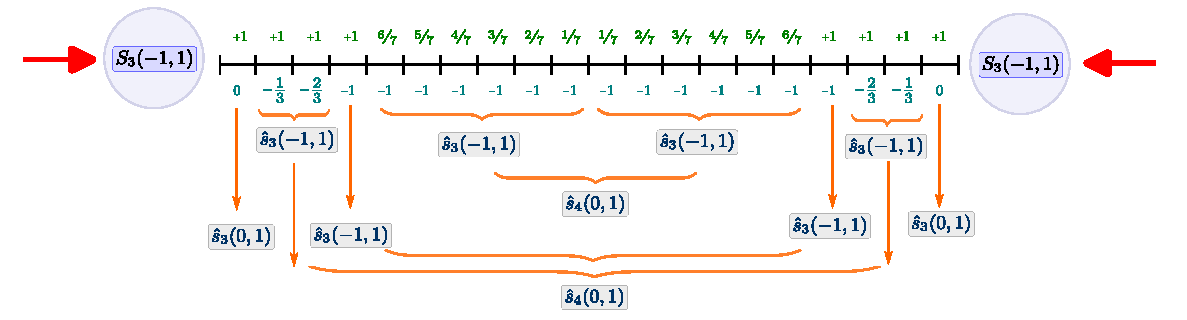
\includegraphics[width=1.0\columnwidth]{interaction-S3.pdf}
	\caption{\footnotesize{\textbf{Fusion de deux nœuds $S_3$.} Produit de fusion de nœuds $S_3$ selon leur type. La flèche rouge représente la force de fusion. Les divisions représentent les vorespaces du plenum.}}
	\label{figure:4-0}
\end{figure}

\begin{multicols}{2}

Le processus se poursuit jusqu'à la formation d'un tore complet.
À noter que notre pauvre électron disparaît totalement.

La particule $S_4$ ne peut être raccrochée à aucune particule du modèle
standard (spin 1, charge nulle), à part peut-être un boson massif
comme le boson Z.

Un calcul de la masse élémentaire du boson Z donne
\begin{equation*}
m_{Z} = \frac{91,188 \cdot 10^6}{2^{32}} = 2,12 \cdot 10^{-2}\,eV/c²
\end{equation*}

La valeur est proche de celle obtenue avec l'électron, donc on peut
dire que c'est un candidat sérieux.

Enfin, les fusions produisent des pseudo-électrons (qui peuvent éventuellement se recombiner en pseudo-bozons Z) et de la pseudo-masse.

\subsubsection{de $S_5$ à $S_7$}

Deux particules $S_4$ fusionnent selon le modèle $S_2$ pour donner la
particule $S_5$, une sorte de super-photon de masse. Là aussi, son spin
de 1 et sa charge nulle en font un candidat au titre de boson Z.
\begin{equation*}
m_{Z} = \frac{91,188 \cdot 10^6}{2^{40}} = 8,3 \cdot 10-5\,eV/c^2
\end{equation*}

Sa masse étant beaucoup trop faible, cette particule n'est
associable avec aucune du modèle standard.

Sur le modèle de fusion de $S_3$, deux particules $S_5$ vont fusionner en
une particule $S_6$, une $S_3$ «géante». On retrouve les propriétés de
l'électron, la charge négative et le spin \R{1}{2}. Les seules particules
du modèle standard candidates pourraient être le muon et le tauon.

Pour le muon:
\begin{equation*}
m_{\mu} = \frac{105,66 \cdot 10^6} {2^{48}} = 3,7 \cdot 10^{-7}\,eV/c^2
\end{equation*}

Pour le tauon:
\begin{equation*}
m_{\tau} = \frac{1,778 \cdot 10^9}{ 2^{48}} = 6,3 \cdot 10^{-6}\,eV/c^2
\end{equation*}

Aucune ne semble assez massive, si l'on considère bien entendu la
référence comme « $S_3$ est l'électron».

Le processus produit encore de nombreux photons.

Le passage à S$_7$ rassemble 7 $S_6$ qui s'enroulent cette fois en tore. Le
processus de fusion suit un processus analogue à celui de la fusion de
$S_3$, à cause de la présence de charges électriques. L'angle solide est
cette fois un $S_6$, qui est un tore à double-hélice. Les
pseudo-particules sont donc des fermions, de la «masse» de $S_6$. Les
$S_6$ doivent aussi se retourner deux à deux pour pouvoir s'emboîter.
$S_7$ est encore candidate pour le muon et le tauon.

Pour le muon:
\begin{equation*}
m_{\mu} = \frac{105,66 \cdot 10^6} {2^{56}} = 1,47 \cdot 10^{-9}\,eV/c^2
\end{equation*}

Pour le tauon:
\begin{equation*}
m_{\tau} = \frac{1,778 \cdot 10^9}{2^{56}} = 2,5 \cdot 10^{-9}\,eV/c^2
\end{equation*}

Il semblerait bien que ce ne soit pas le cas.
\medskip

Le processus de croissance fractale est terminé. Il a produit une
particule hyper-massique $S_7$, des pseudo-particules $S_6$ et $S_3$ et
quantité de photons. Au cours du processus, seules deux particules ont
pu avoir une correspondance dans le modèle standard, à savoir
l'électron ($S_3$) et le boson Z ($S_4$), le photon étant hors-concours.

Est-ce à croire que la loi de croissance fractale ne produit pas nos
particules élémentaires? Il va de soi que non. Le modèle est bien
entendu à replacer dans le cadre de la thermodynamique du Big Bang,
dans les conditions initiales qui ont permis de fusionner des
électrons par exemple, ce qui est impossible dans nos conditions
actuelles. La température et la cinétique des particules sont
extrêmement élevées, ce qui permet d'obtenir des nœuds massifs
impossibles à maintenir dans des conditions plus normales. Il va de soi
que dès que la température baisse, les nœuds, hyper-massifs, ne
peuvent plus tenir et vont tout simplement se dérouler. Si le
processus de fabrication initiale n'avait rien produit d'autres que
ces nœuds, on aurait un simple phénomène de rebond. Mais le processus a
produit des pseudo-particules qui n'attendent que le passage de
véritables particules pour interagir.
\medskip

Étudions donc ce qu'il se passe quand le processus se refroidit, et
donc que les nœuds se défont...

\subsubsection{Déroulement de $S_7$}

Aussitôt que la température décroît suffisamment ($T=T_{S_6}$), le nœud
$S_7$ se déroule en 7 nœuds $S_6$. Les $S_6$ sont de véritables particules,
qui vont pouvoir entrer en collision avec certains pseudo-fermions $S_6$
issus de la fusion précédente.

On a passé un peu vite l'application de la CCG lors de la formation
de $S_7$, quand 7 $S_6$ fusionnent. La section efficace étant cette fois
un nœud $S_6$, l'empilement des pseudo-particules n'est plus le
processus privilégié. En effet, ce processus avait lieu, car les $S_2$
n'étaient topologiquement pas capables de fractionner la masse ou la
charge. Ce n'est pas le cas des $S_6$. Il va donc se créer autant de
pseudo-particules $S_6$ que de fractions possibles, et ce, en double:

\begin{center}
\begin{tblr}{ccc}
	\vnode{$\hat s_6(+1,\R{1}{7})$}  & \vnode{$\hat s_6(+1,\R{2}{7})$} & \vnode{$\hat s_6(+1,\R{3}{7})$} \\
	\vnode{$\hat s_6(+1,\R{4}{7})$}  & \vnode{$\hat s_6(+1,\R{5}{7})$} & \vnode{$\hat s_6(+1,\R{6}{7})$} \\
	\vnode{$\hat s_6(-1,\R{1}{7})$}  & \vnode{$\hat s_6(-1,\R{2}{7})$} & \vnode{$\hat s_6(-1,\R{3}{7})$} \\
	\vnode{$\hat s_6(-1,\R{4}{7})$}  & \vnode{$\hat s_6(-1,\R{5}{7})$} & \vnode{$\hat s_6(-1,\R{6}{7})$} \\
    \vnode{$\hat s_6(+1,\R{+1}{3})$} & \vnode{$\hat s_6(+1,\R{+2}{3})$} &  \\
    \vnode{$\hat s_6(+1,\R{-1}{3})$} & \vnode{$\hat s_6(-1,\R{-2}{3})$} &  \\
    \vnode{$\hat s_6(+1,0)$}    & \vnode{$\hat s_6(-1,0)$}   &  \\
\end{tblr}
\end{center}

Les fractions de masse sont, malgré tout, une aberration topologique
dans un plenum qui ne connaît qu'une unique particule massique. Les
pseudo-particules vont naturellement se réarranger pour retrouver une
masse nominale, tel que 1/7+6/7, 2/7+5/7, \textit{etc}.). On obtient ainsi 3
pseudo-particules massiques \vnode{$\hat s_6(1, 1)$} et 3 \vnode{$\hat s_6(-1,1)$}. Seule la
première peut interagir avec un \node{$S_6(-1,1)$} spontanément libéré par le
dénouement du nœud $S_7$, en donnant une masse pure \node{$S_6(0,1)$}. Cette
dernière peut alors réagir avec les pseudo-particules massives
anti-chirales pour donner des \node{$S_6(1,1)$}.

Il reste à «réduire» les pseudo-particules partiellement chargées. Il
suffit de les associer soit avec une particule \node{$S_6(1,1)$}, soit avec une
\node{$S_6(-1,1)$}. Il reste alors au final:

\begin{center}
\begin{tblr}{cc}
   \node{$S_6(-1, 1)$}  & \node{$S_6(0,1)$}   \\
   \node{$S_6(\R{-1}{3},1)$} & \node{$S_6(\R{1}{3},1)$} \\
   \node{$S_6(\R{-2}{3},1)$} & \node{$S_6(\R{2}{3},1)$} \\
\end{tblr}
\end{center}

\node{$S_6(-1, 1)$} est un nœud stable à cette température et doit attendre que
la température baisse pour se dénouer.

\node{$S_6(0,1)$} est une masse pure. En quelque sorte, c'est une anomalie du
plenum, car à cette température, seule \node{$S_6(-1,1)$} est attendue comme
nœud stable. \node{$S_6(0,1)$} est trop massive pour se dévisser spontanément
quand la température va baisser et dénouer le nœud de référence
\node{$S_6(-1,1)$}. Il faudra attendre une température plus basse pour dénouer
le vissage trop important de ce nœud.

Les particules à charge fractionnaire sont aussi des aberrations du
plenum. Mais avant de regarder comment elles vont réagir, on peut déjà
noter que \node{$S_6(\R{2}{3},1)$} et \node{$S_6(\R{-1}{3},1)$} sont d'excellents candidats pour
les quarks top et bottom. Il est très difficile d'effectuer un calcul
énergétique, car nous n'avons pas encore de règle évidente, à cause des
charges partielles. Toutefois, si l'on considère que la particule
\node{$S_6(1,1)$} est la plus lourde, alors \node{$S_6(\R{2}{3},1)$} la suit immédiatement en
terme de masse. De même, \node{$S_6(\R{-1}{3}, 1)$} s'en trouve assez éloignée et la
différence de masse entre les deux quarks peut ainsi trouver une
explication logique.
\medskip

Revenons à notre déséquilibre de charge. Comme pour le cas de masses
fractionnaires, les particules avec des charges fractionnaires vont
essayer de se rassembler pour retrouver les charges nominales du
plenum, à savoir $+e$ et $-e$. Les quarks top et bottom vont donc s'unir
et la seule façon d'arriver à une charge entière est d'assembler 2 top
et 1 bottom. Il y a plusieurs manières d'assembler ces 3 quarks, mais
la plus naturelle, la plus compatible avec le principe ockhamien, est de
les assembler sur le modèle du $S_3(S_6)$. On verra par la suite que ce
modèle est absolu et qu'on le retrouve partout, y compris dans les
atomes. Les 3 doubles-hélices vont s'enrouler, le bottom «pris en sandwich»,
en formant une seule double-hélice, par la fusion des 3 doubles-hélices. Il y
a donc trois couches dans la double-hélice finale. La charge étant
positive, on appellera cette particule un \textit{méga-proton}, car le collage
va lui donner une stabilité très supérieure à la somme des énergies
unitaires. Il est probable que son énergie se situe bien au-delà des
100\,GeV/c². D'après mes recherches, il n'y a pas de particules de cette
énergie détectées à ce jour.

De même, les \node{$S_6(\R{-2}{3},1)$} et \node{$S_6(\R{1}{3},1)$} restants vont fusionner selon le
même mode, avec le \node{$S_6(\R{1}{3},1)$} pris en sandwich entre les 2
\node{$S_6(\R{-2}{3},1)$}. Cette particule possède une masse élevée, un spin de \R{1}{2}
et une charge négative. C'est un bon candidat pour le lepton tau, un
\textit{méga-électron}.

La masse pure restante, \node{$S_6(0,1)$}, a un spin de \R{1}{2} et ne possède pas
de charge. C'est un bon candidat pour la neutrino tauique.

\subsubsection{Déroulement de $S_6$}

Si la température continue à descendre, elle atteint alors la
température de déroulement de $S_6$, $T_{S_5}$. \node{$S_6(-1,1)$} se déroule alors
classiquement en \node{$S_5(0,1)$}. Les autres $S_6$ précédemment créés sont
trop contraints par leurs structure hors-système et ils ne peuvent se
dérouler à cette étape. Une explication de cette impossibilité
physique est qu'un déroulement d'une charge ou d'une masse partielle
ne peut se faire dans un nœud de type $S_5$, il lui faut une structure
analogue --~auto-similaire~-- pour se transférer.

Tout au plus peut-on dire que ces nœuds se détendent avec
l'abaissement de la température, les rendant de plus en plus fragiles.

\subsubsection{Déroulement de $S_5$}

La température continue de chuter et atteint $T_{S_4}$ la température de
déroulement du nœud $S_5$. C'est l'apparition du boson Z.
Les nœuds $S_6$ précédents continuent de se détendre, mais n'ayant
aucune correspondance nodale à cette température, ils demeurent liés.

Entre le déroulement de $S_6$ et celui de $S_5$, ces nœuds se sont
tellement déroulés que la tension de serrage a suffisamment chuté
pour transformer les quarks précédents. Il se pourrait que le quark top
devienne un quark charm et le quark bottom un quark strange. Ils sont
toujours des structures de type $S_6$. Visuellement, ils sont identiques
à leurs aînés, mais simplement plus gros.

Toutefois, le baryon $\Xi_{cc}^{++}$, observé récemment par une équipe du CERN
au LHC  \cite{cern-lhcb-charmed2022}, laisse penser que le quark s est plutôt un $S_3$ sur-tendu qu'un
$S_6$ relâché. En effet, le baryon $\Xi_{cc}^{++}$ est composé de 2 charm et d'un
down, qui n'apparaîtra que dans la zone de température suivante. Le strange étant
plus lourd, il reste une incertitude sur sa structure réelle.

\subsubsection{Déroulement de $S_4$}

Enfin, la température atteint $T_{S_3}$, la température électronique,
proche de la température actuelle de notre univers. Le nœud $S_4$
précédent libère ses $S_3$ et les électrons réapparaissent.

Cette étape a une énorme incidence sur les $S_6$ en cours de
relâchement. Ils ont enfin une structure auto-similaire qui leur
permet de se dénouer complètement. Tous les $S_6$ se transforment en
$S_3$. Il y a une sorte d'effet avalanche, car un $S_6$ produit $2^{24}$ $S_3$!
Les méga-protons et les tauons, le méga-électrons, vont aussi se
réduire en produisant tous leurs homologues $S_3$:

\begin{center}
	\begin{tblr}{cc}
		\node{$S_3(-1, 1)$}       & \node{$S_3(0,1)$}        \\
		\node{$S_3(\R{-1}{3},1)$} & \node{$S_3(\R{1}{3},1)$} \\
		\node{$S_3(\R{-2}{3},1)$} & \node{$S_3(\R{2}{3},1)$} \\
	\end{tblr}
\end{center}

Le \node{$S_6(\R{-1}{3},1)$} devient donc un quark d \node{$S_3(\R{-1}{3},1)$} et le \node{$S_6(\R{2}{3},1)$} un quark u \node{$S_3(\R{2}{3},1)$}. Les
\node{$S_3(\R{1}{3},1)$} et \node{$S_3(\R{-2}{3},1)$} restants, ne pouvant exister tels quels dans
le plenum, s'associent en triplet, selon le processus évoqué plus
haut, pour former une particule analogue à une forme de $S_3$. C'est le
lepton muon, de charge -e et de spin \R{1}{2}. La masse pure \node{$S_3(0,1)$} est
bien entendu candidate au titre de neutrino muonique.

\subsubsection{Le mot de la fin}

Si l'on était exactement à la température $T_{S_3}$, le processus s'arrêterait
là, mais la température de l'univers doit se situer un peu en-dessous
à l'heure actuelle. La masse pure \node{$S_3(0,1)$}, en tant qu'anomalie du
plenum, va vouloir aussi se délier et la seule issue possible est de
se délier dans un état analogue, qui est celui du plenum. Le \node{$S_3(0,1)$}
va donc avoir tendance à se dénouer en masse pure unitaire \node{$S_0(0,1)$},
c'est-à-dire un vorespace massique. Ce sera notre dernier élément du
modèle standard : le neutrino électronique.

Notez au passage que cette étape résout le problème de la chiralité
unique du neutrino. Si les neutrinos sont «gauches», c'est parce que
le plenum tourne naturellement à gauche, donc en tant qu'élément
unitaire du plenum, le neutrino n'a pas d'autre choix que de s'aligner
sur le sens de rotation des vorespaces.

Mais est-ce la fin pour autant? Si la température était de zéro,
alors le neutrino électronique serait confiné dans son état (on verra
dans le modèle du Big Bang une possible évolution à ce stade). Mais la
température est plutôt proche de $T_{S_3}$, donc le neutrino électronique
va se rassembler avec un anti-neutrino en créant un $S_1$, qui lui-même
va pouvoir éventuellement créer un $S_2$. Étant au seuil inférieur de
$T_{S_3}$, il est probable qu'aucun $S_2$ ne puisse se transformer en $S_3$.

Il se crée donc une certaine quantité de masse pure neutronique \node{$S_0(0,1)$}, de
\node{$S_1(0,1)$} et de \node{$S_2(0,1)$}, qui s'accumule progressivement. Cette
accumulation est une bonne candidate pour la matière noire. Représentant
2/7 des nœuds possibles de la matière, par conservation de la masse,
elle doit représenter 28,6\,\%\ de la matière totale de l'univers. Ce
chiffre correspond aux prévisions actuelles --~qui situe la quantité de masse noire
entre 25\,\%\ et 27\,\%.

À noter que par analogie avec le vorespace, le neutrino est donc le
candidat naturel en tant que monopole magnétique, confirmant ainsi ce
qu'avait montré Georges Lochak. \cite{lochak2002monopole}
\medskip

Bien entendu, il manque encore trois candidats. Faisons un sort aux
bosons $W^{\pm}$. Ce sont clairement des «nœuds impossibles». Ils ont une structure
bosonique, donc un nœud de type $S_1$, $S_2$, ou $S_4$, $S_5$, pèsent très
lourd, donc plutôt un nœud de type $S_4$ ou $S_5$, mais comme ils sont chargés, cette charge 
les rend incompatibles avec les nœuds précédents. En réalité, ces bosons
n'existent pas en tant que tel: ils simulent dans le modèle standard
l'\textit{action naturel du plenum, sa géométrie, qui impose la relation entre
les différents nœuds, selon leurs charges. C'est bien une propriété
intrinsèque du plenum, qui n'a pas besoin d'auxiliaire externe pour se
manifester}.

Enfin, le boson de Higgs est un peu particulier. On a arrêté le modèle
de croissance à $S_7$. Mais en théorie, il est possible de pousser le
modèle au-delà, de manière à créer un «super nœud» $S_1$, construit à partir
des $S_7$. L'angle solide de recouvrement de chacun des assemblages de
$S_7$ est un cercle (un tore en réalité) et devrait donc donner un tore
bosonique de spin 1. Mais ce processus est en réalité impossible, car
la fractalité impose de revenir à l'étape 1, en tant qu'élément
autoconforme, donc de spin 0. C'est par ce processus que le boson de
Higgs apparaît: charge nulle et spin 0, avec une énergie très élevée.

Toutes les particules élémentaires du modèle standard ont été
reconstituées, à l'exception des bosons $W^\pm$, qui sont l'expression de
la nature profonde du plenum.

\subsubsection{La matière baryonique}

Il aurait été dommage de s'arrêter là, sans commencer à introduire la
matière baryonique. On développera toutefois davantage ce point dans
la partie consacrée aux noyaux atomiques.

Pour des raisons de stabilité, aucune structure nouée ne peut exister
dans le plenum en n'étant pas en équilibre, c'est-à-dire en communion
avec la structure du plenum, les vorespaces. Cela force tout nœud
incomplet, c'est-à-dire partiellement chargé ou partiellement
massif, à trouver un moyen de compléter son ou ses manques. Le seul moyen
de complètement est l'association avec un autre nœud partiel. Le modèle du
nœud de référence étant le vorespace, un état $S_3$, l'association doit
privilégier cette forme et c'est la raison pour laquelle les nœuds
partiels s'associent généralement plutôt via la fusion de trois nœuds
partiels.

De même, pour retrouver une analogie de forme $S_3$, les nœuds
s'enroulent les uns dans les autres, autour d'un axe hélicoïdal, afin
de retrouver la forme de la double hélice. C'est cette forme qui donne
la propriété de la particule finale, plutôt que la somme des
propriétés de ses composants.

En effet, quand un proton se forme (par l'association de 2 \node{$S_3(\R{2}{3},1)$}
et 1 \node{$S_3(\R{-1}{3}, 1))$}, on pourrait penser que la valeur du spin vaut \R{1}{2},
car elle est formée de trois nœuds, dont l'un est inversé pour
respecter l'enroulement, le «pas de vis», et que le spin est la somme
de 2 spins \R{1}{2} et d'un spin \R{-1}{2}. 

En réalité, c'est faux, comme le
montre la «crise du spin du proton», car l'éclatement du proton
prouve que la valeur de chacun des spins internes ne participe
que pour environ 25\,\%\ du total final\cite{ashman1988measurement}. C'est bien la forme totale, de
type $S_3$, qui porte la signature principale, de même que c'est la
forme \node{$S_x(-1,0)$} qui porte la charge électrique, que l'on retrouve à
l'échelle du vorespace, ou bien à l'échelle de l'échelle, $2^{24}$ fois
plus grande! Voilà qui devrait clore le débat sur la crise du spin du
proton. \textit{C'est la forme qui porte la caractéristique physique, pas la
somme des composants.}

Le neutron est bien entendu l'autre façon de rassembler les nœuds
restants.

Il reste à comprendre pourquoi le proton et le neutron s'associent.
Cette réponse viendra dans la partie sur le noyau atomique.

Voici un tableau récapitulatif des particules élémentaires selon le
modèle standard de la \PQ:
\vfill

\end{multicols}
\vspace*{-1cm}
\begin{center}
	\begin{longtblr}[
		%theme=widecaption 
		caption={\footnotesize{\textbf{Ordre d'apparition et structures des particules élémentaires}}},
		label = {tblr:5-0-2},
		]{
			colspec={Q[c,m]  Q[c,m] Q[c,m] },
			rowspec={Q[c,m]},
			row{odd}={bg=blue!10!white},
			row{1}={c,mode=text,fg=white,bg=pkcolor, cmd=\textbf}, %cmd=\textbf, blue!80!orange
			rowsep=2pt, colsep=3pt,
			vline{2-Y} = {1}{0.3pt,gray!50},
			vline{2-Y} = {2-Z}{0.3pt,gray!30},
			hline{Z} = {0.1pt,blue},
			% nombre de col début et fin qui apparaissent à chaque page
			% 1 pour le titre par exempel
			rowhead = 1, %rowfoot = 1, 
		}
		
		Température (décroissante)  &   Nœuds                                &   Particules élémentaires   \\
		  $T_{S_6}$                 &     \node{$S_6(\R{2}{3},1)$}           &   Quark top                 \\
		                            &     \node{$S_6(\R{-1}{3},1)$}          &   Quark bottom              \\
		                            &     $t+b+t$                            &   méga-proton (hors modèle) \\
   		                            &     \node{$S_6(\R{-2}{3},1)$}+\node{$S_6(\R{1}{3},1)$}+\node{$S_6(\R{-2}{3},1)$} &   Tau (méga-électron)\\
   		                            &     \node{$S_6(0,1)$}                  &   Neutrino tauique          \\    
		  $T_{S_4}$                 &     \node{$S_4(0,1)$ }                 &   Boson Z                   \\
		  $T_{S_3}$                 &     \node{$S_6(\R{-1}{3},1)$}+\node{$S_3(\R{2}{3},1)$}+\node{$S_3(\R{-1}{3},1))$}   &  Lepton muon\\		  		  
		                            &     \node{$S_6(\R{-1}{3},1)$}          &   Quark d                   \\		  
		                            &     \node{$S_6(\R{2}{3},1)$}           &   Quark u                   \\
		                            &     \node{$S_3(-1,1)$}                 &   Électron                  \\                     
		                            &     \node{$S_3(0,1)$}                  &   Neutrino muonique         \\
		   < $T_{S_3}$              &     \node{$S_2(0,1)$}                  &   Masse noire               \\
		                            &     \node{$S_1(0,1)$}                  &   Masse noire               \\
		                            &     \node{$S_0(0,1)$}                  &   Neutrino électronique (masse noire)  \\
		                            &     \node{$S_0(-1,0)$}                 &   Vorespace (hors modèle)  \\  		    	
		                            	  
		  \end{longtblr}
\end{center}
%\end{multicols}

\begin{multicols}{2}

Il faut compléter ce tableau par la remarque suivante: le photon est une
particule à part, issue de la rupture du plenum, donc d'une rupture
dimensionnelle (brisure de symétrie). Les bosons $W^\pm$, ainsi que le
gluon, n'existent pas en tant que tels, car ils sont l'expression des
contraintes structurelles du plenum.

\subsubsection{Conclusion}

On pourrait presque conclure l'article, puisque l'objectif énoncé
au début, à savoir reconstruire le modèle standard des particules
élémentaires, a été atteint. Il serait pourtant dommage de s'arrêter en si
bon chemin. On va montrer que non seulement la \PQ\ est compatible
avec les autres physiques, mais reconstruire aussi un atome sous
l'angle de la \PQ, proposer un modèle du Big Bang «complet» et
répondre à certains grands problèmes que se posent les physiciens dans
leurs théories respectives.

\subsection{Déplacement dans le plenum}

Il manque encore à ce stade une réponse à la question: «comment se
déplace physiquement une particule dans le plenum?». En effet, la
réponse n'est en rien triviale.

Premièrement, étudions la particule la plus simple, à savoir le
neutrino. C'est une particule massique qui est un constituant naturel
du plenum. Elle est régie par ses lois et, si elle forme techniquement
un bouchon topologique à l'endroit où elle se trouve, elle peut sans
problème se déplacer. Elle se visse donc naturellement dans un
vorespace, selon les règles du plenum, et donc à la cadence du plenum.
\textit{Le neutrino circule donc à la vitesse de la lumière.}

Est-ce que cela viole la relativité restreinte? Non, car le neutrino
est une brique élémentaire: il est un composant de la structure.

Il faut désormais se concentrer sur les autres particules. Ce sont des
nœuds, donc ils doivent circuler tous ensemble pour respecter leur forme
de nœud. Or le déplacement dans le plenum se fait par
auto-réplication. Après un tic du plenum, une particule s'est
reconstituée sur le vorespace suivant. Mais tant qu'elle ne s'est pas
reconstituée, la particule fusionnée liée avec celle qui s'est déplacée
ne peut pas entamer son processus de réplication. Bien entendu, il
n'est pas question de défusionner les objets le temps de faire une
réplication, sinon on observerait une gerbe de photons à chaque
déplacement d'une masse, ce qui ne se voit pas. Et puis le coût
énergétique serait tel qu'un objet perdrait toute sa masse très
rapidement.

Il est plus simple de jouer avec la tension du nœud. La partie
extérieure de la particule va bien se déplacer par auto-réplication,
créant une tension générale dans le nœud. À l'étape d'après, devant le «vide» de
vorespace, la série suivante va se répliquer à son tour, détendant
partiellement le nœud. Et ainsi de suite jusqu'à la dernière série. Puis
on recommence à zéro.\textit{ Un nœud avance donc à la manière d'une chenille.}

Bien entendu, le coût de dispersion de la chenille fait qu'il est
impossible à une particule massive de se caler sur la vitesse de la
lumière, car la chenille serait totalement tendue lors du déplacement. 
Les particules massives de l'univers, autre que les neutrinos, respectent bien 
la relativité restreinte.

\subsection{Les forces dans le cadre de la \PQ}

\subsubsection{La force de gravité}

Il est bon à ce stade de reformaliser proprement la force avec tout ce
qui a été établi précédemment. On a vu que la force appliquait sur le
plenum un phonon de masse selon un processus de 7 pas dans les
derniers retranchements.
\vfill
\end{multicols}

\begin{figure}[H]
%\captionsetup{width=5cm}
\centering
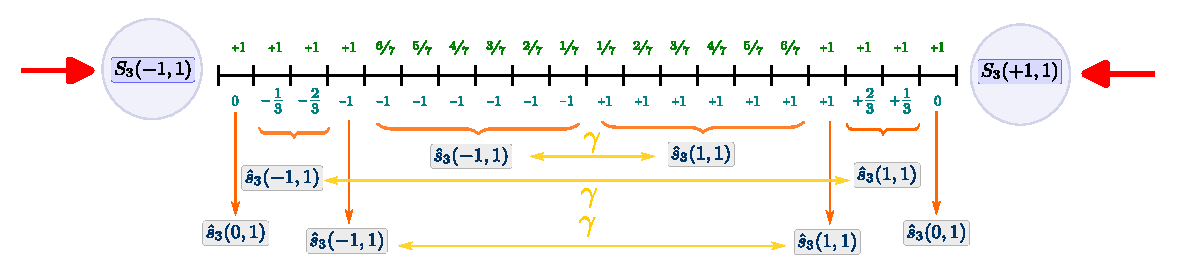
\includegraphics[width=1.0\columnwidth]{interaction-S3-antiS3.pdf}
\caption{\footnotesize{\textbf{Fusion de deux nœuds $S_3$ et anti-$S_3$.} Produit de fusion d'un électron et d'un positon. La flèche rouge représente la force de fusion. Les divisions représentent les vorespaces du plenum.}}
\label{figure:5-0}
\end{figure}

\begin{multicols}{2}

L'interface de contact est l'angle solide sous lequel se présente la
particule massique, qui est généralement une forme de $S_3$ ou de $S_6$.

Selon qu'il se forme des tores ou des $S_3$, le processus de
recouvrement diffère légèrement dans son procédé initial, mais pas
dans sa finalité. Quand des $S_2$ se forment, ils se compactent
d'abord en \vnode{$\hat s_3(0,1)$}, avant d'être éjectés tandis que lorsque ce sont
des \vnode{$\hat s_3(0,\R{i}{7})$}, (pour i allant de 1 à 7) ils sont éjectés tels quels avant de se recombiner en
\vnode{$\hat s_3(0,1)$}.

Chaque couple de \vnode{$\hat s_3(0,1)$} de chaque côté va fusionner sous la poussée
de la gravité, transférant d'un côté l'énergie à l'objet de fusion, le
photon, et de l'autre à l'objet massique à fusionner. Il se crée donc
2 photons et la fusion a récupéré l'énergie de 2 vorespaces.

Le bilan énergétique est que chaque objet massique a un coût de
fusion double d'un point de vue énergétique, un pour l'objet, un pour la
fusion.

On peut donc calculer l'énergie d'un neutrino. Par exemple, l'électron
est composé de $2^{24}$ neutrinos fusionnés, soit
\begin{equation*}
m_{\nu_{fusion}} = \frac {0,511 \cdot 10^6} {2^{24}} = 30,46\,mEV/c²
\end{equation*}

Le neutrino étant le double d'un vorespace, on en déduit
\begin{equation*}
m_{\nu} = 15,23\,meV/c²
\end{equation*}

en accord avec les prévisions du modèle standard qui la situe à une masse inférieure à 0,8\,eV/c².

\subsubsection{La force électrique}

La force électrique concerne donc le phénomène engendré sur le plenum
en présence de deux charges. Il n'existe pas de particules purement
chargée sans masse. Il faut donc ajouter la masse à l'équation du
problème.

Le problème est en réalité similaire à celui résolu lors de l'approche
de deux masses de même signe (\textit{cf.} figure \ref{figure:4-0}). Il avait fallu, pour respecter un peu la
torsion du plenum, retourner une masse pour adapter les chiralités.

Ici, les chiralités opposées sont consubstantielles au problème.

Il se produit des \vnode{$\hat s_3(1,1)$} et des \vnode{$\hat s_3(-1,1)$} qui engendrent des photons,
sans nécessité de coût énergétique. Le processus est inhérent au plenum.

\subsection{Les constantes de la physique à la lumière de la \PQ}

\subsubsection{Temps et masse}

Il va falloir maintenant relier la \PQ\ aux constantes de la physique.
Par construction, par essence pourrait-on dire, la \PQ\ est la
relativité restreinte et on a donc déjà introduit c, la vitesse de
transmission nominale dans le plenum à l'équilibre.

Selon la physique actuelle, la longueur de Planck est la longueur
minimale en-dessous de laquelle la physique actuelle «s'écroule».
Elle est la limite spatiale où la mesure commence. Techniquement, on
peut la voir comme l'étalement spatial de l'objet physique le plus
petit.

Cette définition pose un problème en \PQ, car l'objet le plus petit est
le neutrino, la masse élémentaire. Si cet objet est de la taille de
Planck, c'est-à-dire que le vorespace est de la taille de Planck,
alors le photon parcourt deux fois la taille de Planck sur sa taille,
et il va donc deux fois moins vite que la lumière. On est donc
obligé d'admettre que le vorespace n'a pas la taille de Planck, mais
sa moitié.

Il existe donc \textit{de facto} un objet plus petit que la taille de Planck,
le neutrino. C'est la raison pour laquelle une masse peut aller à la
vitesse de la lumière sans violer la relativité restreinte.
\medskip

On peut désormais calculer quelques valeurs. Par exemple, le tic du
plenum vaut
\begin{equation*}
	\begin{split}
    t_v &= \frac {L_v}{c} = \frac{1}{2} \frac{L_p}{c} \\
        &= 1/2 \times 1,616 \cdot 10^{-35} /299 792 458 \\
        &= 2,695 \cdot 10^{-44}\,s
	\end{split}
\end{equation*}

On a donc $t_v = \R{1}{2}t_p$, ce qui est normal, puisque le vorespace est 2 fois plus petit que la
longueur de Planck.

De plus, la masse du neutrino lié vaut
\begin{equation*}
m_{\nu_{li\acute{e}}} = \frac {0.511 \cdot 10^6}{2^{24}} = 3,045 \cdot 10^{-2}\,eV/c^2
\end{equation*}

Si la masse du photon est bien nulle, on a, pour 2 neutrinos liés, 8
vorespaces de «consommés», soit un rapport de 1 pour 4. La masse du
neutrino est donc 1/4 de la masse liée, soit
\begin{equation*}
m_{\nu}= 7,6\,meV/c²
\end{equation*}

Cette masse est compatible avec les mesures actuelles, qui attendent
une masse du neutrino inférieure à 800\,meV/c².

On a, de fait, une masse unitaire du vorespace de la moitié, soit
$m_v = 3,8\,meV/c²$.

\subsubsection{Le cas de la lumière: et la constante de Planck fut!}

Le cas de la lumière n'a pas été réellement traité jusqu'à présent et
son analyse va permettre de régler bien des détails non encore abordés,
comme la relation entre le photon et les charges électriques. La
création du photon peut laisser croire que le photon que la physique
utilise aujourd'hui est cet objet. Il n'en est rien. Ou du moins, nous verrons qu'il s'agit en réalité d'un
simple sur-ensemble.

En effet, si l'on regarde les choses d'un point de vue mécanique, un
photon de la taille d'un vorespace, et même d'un double-vorespace, ne
peut pas interagir facilement avec un électron, un nœud $2^{24}$ fois plus
grand. Il faudrait qu'il tape dessus selon un processus compliqué pour
justifier une interaction. Il est beaucoup plus simple de
postuler que le photon qui interagit avec l'électron est un objet
d'une taille similaire: il pourra alors s'enrouler naturellement, à
la manière du photon sur le vorespace, puisque l'électron n'est qu'un
vorespace géant. C'est la réalité fractale!

Le photon va donc chercher à adopter le nœud du plenum qui lui
ressemble et qui est stable à l'échelle du plenum. Ce n'est pas un
nœud $S_3$, puisque le photon a un spin de 1. Par construction, c'est un
nœud $S_2$. C'est exactement l'objet recherché, car la taille du nœud
$S_2$ permet un emboîtement parfait autour du nœud $S_3$, le nœud $S_3$
n'étant qu'un nœud $S_2$ «élevé dans la dimension supérieure».

On pourrait s'arrêter là, dire que le processus est consubstantiel au
plenum, et l'admettre. Il peut être intéressant de justifier la
construction de cet objet.

En effet, jusqu'à présent, on a assemblé deux neutrinos via la force
de gravité. Comment assembler deux photons, étant donné que ce sont
des phases pures? Par la phase justement. Le photon a une rotation de
phase naturelle de $2\pi/7$. Deux photons ensemble ne peuvent «être en
phase» qu'en ajustant leur phase! Les deux photons deviennent alors
un unique double photon.

On n'a d'autre part qu'un unique processus pour élaborer notre objet
final: c'est le processus fractal de la \PQ. Le photon doit le suivre
et créer d'abord un nœud $S_1$ avant d'arriver au nœud $S_2$. Ce processus
pose un problème technique: un nœud $S_1$ est un «cercle» de photons.
Comment courber des photons?

Heureusement, la gravité vient sauver l'alignement rectiligne de
photons. Le photon est un \textit{surfeur phonique} et aussitôt qu'il rencontre
une masse, il suit le talweg de néguentropie: la présence d'un
neutrino, avec son phonon heptagonal, va forcer les groupes
rectilignes de photons à «orbiter» autour du neutrino et à
s'assembler. Le nœud $S_1$ prend alors naissance autour du neutrino.
L'étape suivante consiste à assembler 7 nœuds ensemble. C'est facile,
car deux nœuds $S_1$ décalés de $2\pi/7$ s'emboîtent parfaitement. Mais
comme, spatialement, la place est déjà occupée sur un vorespace, il
faut décaler le premier cercle de photon d'un demi-vorespace, selon
l'organisation des brins d'ADN du plenum. Il y a bien entendu 7
décalages avant de boucler un enroulement complet. Il faut ensuite
recommencer 7 fois avec l'ensemble précédent: le premier ensemble de
$2^7$ photons est prêt à rencontrer un homologue pour former l'objet
final.

Le vecteur de fusion doit évoluer à ce stade, car le neutrino n'a pas
la forme d'onde nécessaire pour déplacer le nouvel objet dans deux
directions d'espace différentes. Il passe alors la main à
l'électron. Ce dernier, de forme $S_3$, produit une onde heptagonale
plus complexe, selon deux axes perpendiculaires. Un nœud $S_1$ va
prendre la direction d'un axe (toujours en surfant phoniquement) et le
second l'autre, jusqu'à la rencontre: l'objet est alors créé! C'est
un nœud $S_2$.
\medskip

On peut montrer que ce nœud est le photon de la physique moderne en
calculant sa longueur d'onde.

Ce nœud est en effet une image fractale du photon élémentaire. Ce dernier a une
longueur d'onde de la longueur de Planck $L_p$. La longueur fractale,
passée par deux dimensions, sera donc de $7\times 7$ fois la longueur de
Planck.

Il faut soustraire à cette longueur l'épaisseur du photon conforme, car ce
dernier n'est plus une simple phase, ayant grossi par fractalité deux
fois: il faut donc lui retirer chaque épaisseur fractale, soit 1 pour
la première et 7 pour la seconde. La longueur d'onde du photon
homologue est donc de $41 \cdot L_p$.
\begin{equation*}
\lambda_{\gamma} = 41 \cdot L_p = 41 \cdot 1,616255.10^{-34} = 6,6266.10^{-34}\,m
\end{equation*}

\textbf{C'est exactement la constante de Planck !}
\medskip

La formule $E=h\nu$ est donc le paquet d'énergie minimale pour un cycle
de période, soit une fréquence de 1. C'est «E=h», c'est-à-dire
$E=6,6.10^{-34}\,J$.
\medskip

Comme c'est un nœud de type $S_2$, il est composé de $2^{15}$ photons
élémentaires (il y a 2 photons par vorespace assemblé), on peut donc
calculer la masse de ce dernier:
\begin{equation*}
m_{\gamma_{el}} = \frac {E_{unitaire}} {2^{15}} = 1,91.10^{-38}\,J = 1,65.10^{-57}\,eV/c²
\end{equation*}

\textit{Le photon élémentaire a donc bien une masse, contrairement à ce
qu'affirme le modèle standard de la physique.} Toutefois, ce dernier
n'est en rien absurde, dans le sens où cette masse est si faible que la
considérer comme nulle est une approximation proche de la réalité.

Le fait que le photon ait donc une masse de cette importance est peu
impactant pour la physique, car

\begin{itemize}
	\item elle est totalement négligeable dans l'énergie de liaison;
	\item elle n'est pas sensible, même à l'échelle de l'univers, car sa
	demi-longueur d'onde est à l'échelle de la moitié de l'univers (\textit{cf}.
	le modèle du Big Bang).
\end{itemize}


Il n'empêche que le photon a bien une masse, comme l'avait aussi prévu
de Broglie, qu'il avait calculée autour de $10^{-61}\,eV/c²$\cite{debroglie1956tentative}. La limite
cosmologique propose aussi une valeur autour de $10^{-62}$.
\medskip

La conclusion s'impose d'elle-même: la vitesse du photon ne peut être
rigoureusement égale à «celle de la lumière». La différence de ces
vitesses est si petite qu'elle n'est pas mesurable. Il serait
passionnant de trouver une expérience permettant de la mettre en
évidence. La plus simple serait de trouver une source d'émission
située à l'opposée de notre position dans l'univers et de mesurer la
différence de temps à l'arrivée. Mais faire fi des contingences
rencontrées sur le parcours est un défi de taille!

\textit{Stricto sensu}, il faudrait donc renommer la vitesse de la lumière en
vitesse $v_p$ du plenum, tout en considérant désormais constant le
rapport $v_p/c$.

\subsubsection{L'interaction électromagnétique}

Il faut étudier les conséquences de ce qui précède. On appellera
désormais photon le photon homologue et photon élémentaire le photon
de base.

Le photon est adapté au processus d'enroulement autour d'un nœud $S_3$
homologue dimensionnellement. C'est le cas de l'électron, qui est
l'homologue du vorespace, mais qui est composé de neutrinos.

Toutefois, si le photon élémentaire «traverse» le vorespace sans
sourciller, --~bien qu'il faudrait \textit{stricto sensu} désormais tenir
compte du fait que ce n'est pas rigoureusement exact~--, ce n'est pas le cas
du photon avec l'électron. En effet, si l'électron est l'image
conforme du vorespace, il ne l'est pas structurellement: l'électron
est composé de neutrinos, donc de masse. Il doit avoir rigoureusement
la structure du vorespace, donc être un nœud \node{$S_3(-1,0)$} pour avoir la
propriété de charge, mais il est massique et a donc une masse: c'est
un nœud \node{$S_3(-1,1)$}. 

Comme il s'agit d'un nœud \node{$S_3(-1,1)$}, il a au moins une hélice
mobilisée (on justifiera la répartition des rôles des hélices à la fin de ce chapitre) et c'est bien une turbine autour de laquelle va pouvoir
s'enrouler le photon. Mais si la largeur finale est toujours la
largeur maximale, la pale est tout de même très légèrement déformée
par la masse --~on peut la voir comme aplatie par la gravité~--, et le
photon va buter sur cet étage final, sans pouvoir finir son
enroulement, comme il le faisait pour un vorespace. En quelque sorte, le photon n'a
plus assez de place pour passer et il s'écrase contre le mur de la
pale.

Toute l'énergie du photon se transfère alors en 7~pas à l'électron.
L'électron est un nœud stable, qui ne peut modifier sa structure sans une
violente énergie de transformation. L'énergie du photon étant trop
faible pour impacter la structure \textit{in se} du nœud, elle va devoir se
disperser autrement: incapable d'augmenter sa vitesse de rotation,
l'électron va transférer cette énergie dans sa vitesse de translation,
son exergie, par pure conservation de l'énergie. L'impulsion du
photon, en rotation, se transforme en impulsion de translation. C'est
la loi de Noether.

Le processus n'est pas sans conséquence: la transmission se fait à la
fréquence du photon, soit en 1/h, c'est-à-dire à $1,6 \cdot 10^{27}\,Hz$, soit
$6,6 \cdot 10^{-34}$ seconde. L'électron accélère pendant ce bref instant pour
changer de vitesse, et donc de position. À l'échelle microscopique,
parce que la physique mesure les caractéristiques avec une longueur
d'onde de l'ordre du photon, \textit{il donne l'impression de disparaître et
d'apparaître à un autre endroit, en ayant changé de vitesse au nouvel
endroit.} En réalité, la loi d'action-réaction a été scrupuleusement
respectée: en conséquence, le principe fondamental de la dynamique
aussi.

Toutefois, \textit{ce principe est désormais quantifié}. L'accélération, comme
la décélération, ne peut s'effectuer que par quantum de photon, selon
un quantum de temps. À l'échelle microscopique, le phénomène n'est
déjà plus sensible à l'aune de nos moyens expérimentaux.

Par conservation de l'énergie, l'électron décélérant doit céder un
quantum d'énergie éqivalent à celui d'un photon (pour une décélération
quantique d'une unité). Un électron qui ralentit émet donc un photon.
Là encore, il change de position «instantanément» selon nos
appareils de mesure. Il faudrait étudier par quel processus mécanique
le photon apparaît dans ce cadre. C'est sans doute un phénomène
inverse de l'onde de choc du mur du son: en ralentissement, l'onde
devant l'objet perd sa pression et se détend: le photon est le «boum» phonique du «mur du phonon».

Quoi qu'il en soit, ce processus sera éclairant pour illustrer une partie du modèle
atomique qui sera développé par la suite.

Enfin, c'est parce que le dernier pas de vis bloque le passage du
photon que l'interaction entre le photon et l'électron est inévitable.

Si l'on prend une masse équivalente à l'électron, donc un nœud
\node{$S_3(0,1)$}, alors le photon ne va pas buter sur le dernier pas, car la
contrainte de nœud, répartissant l'entropie entre les états 0 jusqu'à
64, va mettre en branle les deux vis internes, transformant les pales,
et laissant assez de place pour que le photon puisse passer.
Paradoxalement, le nœud $S_3$ massique joue le rôle du vorespace à
l'échelle fractale. Ce paradoxe s'explique par le fait que le plenum
n'est plus tout à fait une structure fractale, puisque son énergie
initiale n'a pas été suffisante pour conserver toutes les propriétés
fractales (\textit{cf.} le modèle du Big Bang). Techniquement, le photon a
d'ailleurs très peu de chance de traverser la matière, autre que le
neutrino pure, car l'onde de masse devrait le dévier.

\textit{Le photon est donc bien le vecteur de l'interaction électromagnétique.}

Enfin, on a une cartographie assez fine de l'électron. C'est un nœud
$S_3$ de dimension de la demi-longueur d'onde du photon le long de son pas de vis du double, donc de 42 vorespaces, soit 21 longueurs de Planck. Le diamètre de la «tête de vis» correspond à
celui du cercle du photon, soit un périmètre de $2^7$ photons
élémentaires faisant une longueur de Planck chacun, soit un diamètre
de $2^7 \cdot L_p/\pi$.

Il faut maintenant « habiller » l'électron de l'épaisseur de sa dimension, en multipliant chaque dimension par $2^{16}$. Les dimensions externes de l'électron sont donc $2^{23} \cdot L_p/\pi$ pour le diamètre de la tête, soit $4,3 \cdot 10^{-29}\,m$.

 L'électron est donc une toupie 4 fois plus large que
haute. C'est une turbine «très plate». 

\subsubsection{La formule de de Broglie}

Une conséquence du fait que le déplacement d'un objet soit quantifié
par quantum d'énergie va nous permettre d'arriver à la célèbre formule
de de Broglie.

Il faut revenir à la manière dont se déplace un objet: par
auto-reproduction chenillée. Un objet de longueur caractéristique L va
donc se déplacer à un temps caractéristique de L/c.

L'objet lui-même engendrant une onde unique le caractérisant, par
analogie, l'onde se déplace aussi à ce temps caractéristique. L'onde
ayant une longueur caractéristique différente, sa longueur d'onde
$\lambda$, son propre temps caractéristique vaut $\lambda$/c. La longueur
d'onde est donc égale à la longueur caractéristique de l'objet
physique, ce qui n'est pas surprenant, puisque que c'est cette
caractéristique qui imprime son empreinte dans le plenum.

Or on sait désormais que pour faire avancer l'objet d'un quantum d'impulsion,
 il lui faut un quantum d'énergie correspondant à h. L'objet
ayant une dimension caractéristique de $\lambda$, il lui faut $\lambda/h$
quanta pour déterminer son impulsion,

soit
\begin{equation*}
   p = \frac {h}{\lambda}
\end{equation*}

Le raisonnement est proche de celui de de Broglie qui a
«synchronisé» les vitesse de phase et de groupe entre l'objet
quantique (un électron qu'il considérait comme indéformable) et son
onde-pilote, idée qu'il considérait d'ailleurs comme la plus
importante de toutes ses découvertes scientifiques.\cite{debroglie1963etude}

\subsubsection{La constante de structure fine}

En réalité, il s'en faut de peu que le photon puisse passer lorsqu'il
tente de traverser un électron. La différence d'épaisseur qui dépasse
de l'enroulement est très faible : elle vaut environ 7 millièmes de
l'ensemble. C'est évidemment $\alpha$, la constante de structure fine\footnote{dont l'importance est telle que l'auteur a choisi de numéroter les différentes versions de ce document selon les décimales de cette constante.}.
Avant de se pencher plus en avant sur la façon de la déterminer,
observons ce qu'il se passe à l'échelle du plenum quand un photon
élémentaire traverse un vorespace.

Ce dernier, en tant qu'aberration topologique, est obligé de sauter un
pas sur deux du vorespace, ce qui fait qu'il a besoin de 2
vorespaces pour se dérouler totalement.

Techniquement, le photon élémentaire de lumière glisse à la vitesse c
(du moins, selon une approximation très raisonnable), en épousant les
formes du vorespace, même s'il en saute une sur deux. Ces formes
dépendent de deux paramètres : la largeur de la pale, --~«sa
surface»~--, et son inclinaison, la première se rapportant à la
charge magnétique et la seconde à la charge électrique. Il existe donc
une relation directe liant les 3 caractéristiques.

Appelons $\epsilon$ la caractéristique d'inclinaison et $\mu$ celle de la
largeur de la pale inclinée. $\epsilon$ traduit une charge linéaire (une
charge par longueur) tandis que $\mu$ traduit un champ magnétique (une
unité de champ magnétique, qui correspond à une longueur parcourue par
un flux de charge, donc des charges par unité de temps). Le produit
des nœuds donne l'inverse d'une vitesse au carré. On peut donc relier
ces trois grandeurs en retrouvant la célèbre formule :
\begin{equation*}
c² = \frac{1} {\epsilon \cdot \mu}
\end{equation*}

On a donc, par rapprochement avec la physique actuelle,
\begin{equation*}
	\left\{
	\begin{split}
		\epsilon &= \epsilon_0 \\
		\mu      &= \mu_0
	\end{split}
	\right.
\end{equation*}

On peut enfin donner un sens à une absurdité de la physique qui
prétend sans sourciller que le vide existe$\ldots$ et qu'il a une
permittivité non nulle.

Donc soit la permittivité est nulle et le vide est bien vide, soit la
permittivité n'est pas nulle et le vide n'est pas vide. Heureusement,
le plenum est là pour sauver l'ontologie de la permittivité!
\medskip

Au niveau du vorespace, on a désormais un moyen de mesurer le
flux photonique élémentaire, en reliant la vitesse du photon
élémentaire aux caractéristiques électromagnétiques du vorespace.

Il faut maintenant transposer ce mécanisme au photon et à l'électron.

En réalité, on pourrait penser que puisque les structures du vorespace et de l'électron sont identiques, les effets mécaniques d'emboîtements seraient identiques. C'est exact. À un détail près: l'électron n'est pas auto-similaire au vorespace, mais au neutrino. Il faut donc comparer finement le vorespace et le neutrino pour sentir ce qu'il se passe de différent entre les deux.

Jusqu'à présent, on ne s'est pas trop concentré sur le rôle effectif de chacune des hélices de la « turbine » vorespace ou neutrino. En fait, leur rôle est spécifique: l'une s'occupe exclusivement de la charge, tandis que l'autre s'occupe de la masse. Le fait qu'elles soient contraintes ensemble explique bien la nature couplée de ces interactions.

D'autre part, la contrainte du plenum fait que, et le vorespace et le neutrino, doivent s'imbriquer dans le système, donc \textit{toujours avoir une vitesse de rotation compatible avec leurs voisins}. Or on a montré que la vitesse du neutrino était le double de celle du vorespace. Techniquement, si c'était rigoureusement le cas, le neutrino ne pourrait s'insérer dans le plenum sans tout faire exploser!

La solution ockhamienne consiste à utiliser l'autre hélice, celle de la charge, pour agir à la place de celle de la masse. Comme les hélices peuvent avoir une rotation indépendante, c'est possible: on a donc une rotation pour la masse et une rotation pour l'emboîtement, grâce à l'hélice de la charge, qui, elle, doit tourner à la vitesse du vorespace, donc à la vitesse de $\omega_v$. 

Le vorespace tournant dans le sens lévogyre, la seule solution pour l'hélice de masse du neutrino est de tourner dans l'autre sens. Pour obtenir une moyenne de $(-)2 \omega_v$, il lui faut elle-même tourner à $(+) 3 \omega_v$.

On peut extraire une propriété générale du plenum à partir de cette constation:

\begin{mybox}[breakable,colback=blue!10, colbacktitle=pkcolor]{Propriété}
	La composition des mouvements de rotation des doubles-hélices d'un vorespace ou d'un neutrino doit toujours fournir au moins une rotation unitaire dans le sens lévogyre pour les états stationnaires.
\end{mybox}
\medskip

On peut alors fabriquer un tableau des propriétés de chacune des hélices en fonction des états du vorespace et du neutrino:
\vspace*{-0.5cm}
\begin{center}
	\begin{longtblr}[
		%theme=widecaption 
		caption={\footnotesize{\textbf{Vitesse de rotation relative des hélices du vorespace et du neutrino}}},
		label = {tblr:7-0},
		]{
			colspec={Q[c,m]  Q[c,m] Q[c,m] Q[c,m] Q[c,m]},
			rowspec={Q[c,m]},
			row{odd}={bg=blue!10!white},
			row{1-2}={c,mode=text,fg=white,bg=pkcolor, cmd=\textbf}, %cmd=\textbf, blue!80!orange
			rowsep=2pt, colsep=3pt,
			vline{2-Y} = {1}{0.3pt,gray!50},
			vline{2-Y} = {2-Z}{0.3pt,gray!30},
			hline{Z} = {0.1pt,blue},
			% nombre de col début et fin qui apparaissent à chaque page
			% 1 pour le titre par exempel
			rowhead = 1, %rowfoot = 1, 
		}
		\SetCell[r=2]{c} États  & \SetCell[c=2]{c} Hélice 1 (charge) && \SetCell[c=2]{c} Hélice 2 (masse) \\
                                & vorespace                           & neutrino              & vorespace    & neutrino           \\
                0-20            &    -1                               &    -1                 &     0        &   0                \\
               21-42            &  \Ru{-}{2}{3}{} à \Ru{-}{1}{3}{} &   -1                 &    \Ru{-}{1}{7}{} à \Ru{-}{6}{7}{}   &  \Ru{}{3}{7}{} à \Ru{}{18}{7}{}     \\
               43-45            &    0       &    -1                 &     -1        &   +3                \\    
	\end{longtblr}
\end{center}

On remarque quelque chose d'étrange. Il n'est pas possible d'initier une rotation à $-1$ pour l'hélice de masse du neutrino, sinon la variation en pas de 7 jusqu'à la rotation $+3$ passerait par zéro, ce qui n'a pas de sens physique (il y aurait une inversion de chiralité au cours des états 21 à 42).  Seule son hélice de charge doit porter cette valeur. Mais comme elle la porte aussi au final, sa vitesse de rotation reste constante!

Il ne faut pas interpréter cette bizarrerie plus que dans le domaine d'existence du neutrino. Le neutrino est le nœud \node{$S_0(0,1)$}, c'est-à-dire l'état complet de 0 à 64. Le fait qu'il ait une charge apparente dans son état 0 à 20 vient du fait que le neutrino n'est pas né de rien, mais du «vissage» du vorespace (\textit{cf}. le modèle du Big Bang). La charge électrique disparaît aussitôt que l'énergie se repartit sur le reste des états, car seule la structure \node{$S_0(-1,0)$} porte la caractéristique de la charge électrique $-e$.

D'autre part, il faut bien comprendre \textit{comment} se construit le magnétisme --~ou la masse~-- du neutrino. Le neutrino est un vorespace plus vissé, mais il reste un vorespace. Son incorporation dans le plenum ne lui laisse que peu de choix pour sa forme: il doit se conformer topologiquement à ses voisins vorespaces. En clair, ses surfaces de pale ne peuvent différer de celles de ses voisins: la seule liberté du neutrino reste dans \textit{l'épaisseur} de la pale. Il exploite donc toute l'épaisseur possible, ce qui fige la forme globale. En ne laissant qu'une fine place pour l'emboîtement, la pale épaisse occupe tout le reste du volume, sans laisser de liberté de mouvement à la pale. Elle ne peut donc en particulier plus s'incliner: de fait, sa charge reste constante. Cette contrainte explique donc la valeur constante de la charge apparente du neutrino.

On constate donc une différence notable entre le fonctionnement des hélices de chacun des objets:
\vfill

%\vspace*{-0.5cm}
\begin{center}
	\begin{tikzpicture}
		\begin{axis}[
			width=\columnwidth,          % <-- largeur exacte de la page
			height=0.55\columnwidth,     % hauteur proportionnelle (tu peux ajuster)
			%width=14cm,
			%height=9cm,
			xlabel={Masse (en saut de 1/7)},
			%
			ylabel={Vitesse relative},
			title={Compétition de masse neutrino-vorespace},
			xmajorgrids=true,
			ymajorgrids=true,
			grid style=dashed,
			%ymode=log,                  % <--- échelle logarithmique sur l'axe y
			%log basis y=10,
			ymin=-1.5,                   % pour éviter le log(0)
			ymax=3.5,
			xlabel style={font=\small},
			ylabel style={font=\small},
			title style={font=\bfseries},
			tick label style={font=\small},
			legend pos=north west,
			]
			
			% Données (x = indice, y = valeur)
			\addplot[
			color=blue,
			thick,
			mark=*, 
			mark size=1.5pt,
			] coordinates {
				(0,0)
				(3,3/7)
				(6,6/7)
				(9,9/7)
				(12,12/7)
				(15,15/7)
				(18,18/7)
				(21,21/7)
			};
			\addlegendentry{neutrino}
			\addplot[
			color=red,
			thick,
			mark=*, 
			mark size=1.5pt,
			] coordinates {
				(0,0)
			 	(3,-1/7)
			 	(6,-2/7)
			 	(9,-3/7)
			 	(12,-4/7)
			 	(15,-5/7)
			 	(18,-6/7)
			 	(21,-7/7)
			 };   
			\addlegendentry{vorespace}
			
		\end{axis}
	\end{tikzpicture}
\end{center}
%\vspace*{-0.5cm}
\begin{center}
	\begin{tikzpicture}
		\begin{axis}[
			width=\columnwidth,          % <-- largeur exacte de la page
			height=0.55\columnwidth,     % hauteur proportionnelle (tu peux ajuster)
			%width=14cm,
			%height=9cm,
			xlabel={Masse (en saut de 1/3)},
			%ylabel={Vitesse relative},
			title={Compétition de charge neutrino-vorespace},
			xmajorgrids=true,
			ymajorgrids=true,
			grid style=dashed,
			%ymode=log,                  % <--- échelle logarithmique sur l'axe y
			%log basis y=10,
			ymin=-2.0,                   % pour éviter le log(0)
			ymax=1.0,
			xlabel style={font=\small},
			ylabel style={font=\small},
			title style={font=\bfseries},
			tick label style={font=\small},
			legend pos=north west,
			]
			
			% Données (x = indice, y = valeur)
			\addplot[
			color=blue,
			thick,
			mark=*, 
			mark size=1.5pt,
			] coordinates {
				(0,-1)
				(7/7,-1)
				(14/7,-1)
				(21/7,-1)
			};
			\addlegendentry{neutrino}
			\addplot[
			color=red,
			thick,
			mark=*, 
			mark size=1.5pt,
			] coordinates {
				(0,-1)
				(7/7,-2/3)
				(14/7,-1/3)
				(21/7,0)
			};   
			\addlegendentry{vorespace}
			
		\end{axis}
	\end{tikzpicture}
\end{center}

Un photon étant un révélateur entropique, il va être sensible à la disparité des états internes de chacun des objets et ne pas réagir de la même façon suivant les états. Il traversera le vorespace, mais sera bloqué dans l'électron. La différence entre les deux est minimale --~c'est la constante de structure fine $\alpha$~--, mais suffisante pour changer les règles du jeu de l'interaction du photon avec les nœuds de type $S_3$.

Or la masse est duale avec le champ magnétique: c'est le flux $\Phi$ de l'électromagnétisme. On peut donc voir la répartition des valeurs de masse comme une répartition duale des valeurs de charges magnétiques du monopole associé. En ramenant les charges à des valeurs uniquement positives, on a donc:

%\vspace*{-1.0cm}
\begin{center}
	\begin{tikzpicture}
	\begin{axis}[
		width=\columnwidth,          % <-- largeur exacte de la page
		height=0.55\columnwidth,     % hauteur proportionnelle (tu peux ajuster)
		xmin=0, xmax=1.05,
		ymin=0, ymax=1.15,
		grid style=dashed,
		%xlabel={Position \( x \)},
		%ylabel={Hauteur},
		title={Vorespace: charge électrique vs flux magnétique},
		grid=major,
		legend pos=north west,
		legend style={font=\tiny},
		title style={font=\bfseries\small},
		% === Configuration de l'axe x en fractions de 1/7 ===
		xtick={1/7,2/7,3/7,4/7,5/7,6/7,7/7},
		xticklabels={
			\( \frac{1}{7} \), \( \frac{2}{7} \), \( \frac{3}{7} \), 
			\( \frac{4}{7} \), \( \frac{5}{7} \), \( \frac{6}{7} \), \( \frac{7}{7} \)
		},
		xticklabel style={font=\small}, % rotate=45, anchor=east}, % pour éviter le chevauchement
		ytick={1/3, 2/3, 3/3},
		yticklabels={
				\( \frac{1}{3} \), \( \frac{2}{3} \), \( \frac{3}{3} \), 
		},
		yticklabel style={font=\small}, 
		]
		% ==================== Série 1/3 : barres larges (largeur = 1/3) ====================
		\addplot+[ybar, bar width=1/3, fill=blue!40, draw=blue!70, thick, opacity=0.75] 
			coordinates {
				(1/6,  1)   % centre de la première barre
				(1/2,  2/3)   % centre de la deuxième barre
				(5/6,  1/3)     % centre de la troisième barre
				};
		% ==================== Série 1/7 : barres étroites (largeur = 1/7) ====================
		\addplot+[ybar, bar width=1/7, fill=red!40, draw=red!70, thick, opacity=0.55] 
			coordinates {
				(1/14, 1/7)
				(3/14, 2/7)
				(5/14, 3/7)
				(7/14, 4/7)
				(9/14, 5/7)
				(11/14,6/7)
				(13/14,1)
				};
		\legend{charge électrique, flux magnétique};
		\node[color=red] at (2/28, 0.06) {\R{1}{7}};
		\node[color=red] at (6/28, 0.06) {\R{2}{7}};
		\node[color=red] at (10/28, 0.06) {\R{3}{7}};
		\node[color=red] at (14/28, 0.06) {\R{4}{7}};
		\node[color=red] at (18/28, 0.06) {\R{5}{7}};
		\node[color=red] at (22/28, 0.06) {\R{6}{7}};
		\node[color=red] at (26/28, 0.06) {\R{7}{7}};
		\node[color=blue] at (0.2, 0.4) {1};
		\node[color=blue] at (0.5, 0.4) {\R{2}{3}};
		\node[color=blue] at (0.85, 0.21) {\R{1}{3}};
		\end{axis}
		\end{tikzpicture}
\end{center}
%\vspace*{-1.5cm}
\begin{center}
	\begin{tikzpicture}
		\begin{axis}[
			width=\columnwidth,          % <-- largeur exacte de la page
			height=0.55\columnwidth,     % hauteur proportionnelle (tu peux ajuster)
			xmin=0, xmax=1.05,
			ymin=0, ymax=3.15,
			grid style=dashed,
			%xlabel={Position \( x \)},
			%ylabel={Hauteur},
			title={Neutrino: charge électrique vs flux magnétique},
			grid=major,
			legend pos=north west,
			legend style={font=\tiny},
			title style={font=\bfseries\small},
					xtick={1/7,2/7,3/7,4/7,5/7,6/7,7/7},
			xticklabels={
				\( \frac{1}{7} \), \( \frac{2}{7} \), \( \frac{3}{7} \), 
				\( \frac{4}{7} \), \( \frac{5}{7} \), \( \frac{6}{7} \), \( \frac{7}{7} \)
			},
			xticklabel style={font=\small},
			]
			% ==================== Série 1/3 : barres larges (largeur = 1/3) ====================
			\addplot+[ybar, bar width=1/3, fill=blue!40, draw=blue!70, thick, opacity=0.75] 
			coordinates {
				(1/6,  1)   % centre de la première barre
				(1/2,  1)   % centre de la deuxième barre
				(5/6,  1)     % centre de la troisième barre
			};
			
			% ==================== Série 1/7 : barres étroites (largeur = 1/7) ====================
			\addplot+[ybar, bar width=1/7, fill=red!40, draw=red!70, thick, opacity=0.45] 
			coordinates {
				(1/14, 3/7)
				(3/14, 6/7)
				(5/14, 9/7)
				(7/14, 12/7)
				(9/14, 15/7)
				(11/14,18/7)
				(13/14,21/7)
			};
			\legend{charge électrique, flux magnétique};
			\node[color=red] at (2/28, 0.15) {\R{3}{7}};
			\node[color=red] at (6/28, 0.15) {\R{6}{7}};
			\node[color=red] at (10/28, 0.15) {\R{9}{7}};
			\node[color=red] at (14/28, 0.15) {\R{12}{7}};
			\node[color=red] at (18/28, 0.15) {\R{15}{7}};
			\node[color=red] at (22/28, 0.15) {\R{18}{7}};
			\node[color=red] at (26/28, 0.15) {\R{21}{7}};	
		\end{axis}
	\end{tikzpicture}
\end{center}

Pour le vorespace, la charge magnétique est induite: elle est le résultat de la présence d'une charge électrique. En revanche, pour le neutrino, la charge magnétique est intrinsèque et la charge électrique est induite. Le neutrino est le seul véritable monopole magnétique\footnote{Un nouvel axe d'approche pour capturer des neutrinos serait de les faire dévier dans un champ magnétique.}.

Il n'est pas nécessaire, à l'instar du monopole magnétique de Dirac, d'inventer une quelconque «ligne de Dirac» pour décrire le champ du monopole, car le phonon de charge (magnétique), en tout point équivalent au phonon de masse, décrit totalement le champ.

On a ici le flux qui varie par saut entier. On a donc

\begin{equation*}
	\Phi_m = \sum_{i=1}^{7} \vec{B_i} \cdot \vec{S_i} = \mu_0 q_m
\end{equation*}
soit
\begin{equation*}
	B_i S_i = \mu_0 q_{m_i}
\end{equation*}

Or, les surfaces de pale varient proportionnellement selon un rapport de \R{1}{7}:
\begin{equation*}
	S_i = \frac{i}{7} S_0 = \frac{i}{7} \pi \frac{L_p^2}{2}
\end{equation*}

d'où
\begin{equation*}
	q_{m_i} \mu_0 = \frac{i}{7} B_i S_0
\end{equation*}

Soit
\begin{equation*}
	\left\{
	\begin{split}
		\mu_0  &\propto S_0  \\ 
		q_{m_i}&\propto \frac{i}{7} B_i 
	\end{split}
	\right.
\end{equation*}

La perméabilité magnétique est bien proportionnelle à la surface de la pale et la charge magnétique est quantifiée. On retrouve donc sans surprise la quantification de la charge magnétique de Dirac, les mesures de l'effet Hall quantique \cite{klitzing1980new} et la solution trouvée est proche du soliton de Chern-Simons \cite{jackiw1990solitons}.

\begin{center}
	\begin{tikzpicture}
		\begin{axis}[
			width=\columnwidth,          % <-- largeur exacte de la page
			height=0.95\columnwidth,     % hauteur proportionnelle (tu peux ajuster)
			xmin=0, xmax=1.05,
			ymin=-1.5, ymax=3.15,
			grid style=dashed,
			%xlabel={Position \( x \)},
			%ylabel={Hauteur},
			title={Compétition neutrino vorespace},
			grid=major,
			legend pos=north west,
			legend style={font=\tiny},
			title style={font=\bfseries\small},
			xtick={1/7,2/7,1/3,3/7,4/7,2/3,5/7,6/7,7/7},
			xticklabels={
				\( \frac{1}{7} \), \( \frac{2}{7} \), \( \frac{2}{3} \), \( \frac{3}{7} \), 
				\( \frac{4}{7} \), \( \frac{2}{3} \), \( \frac{5}{7} \), \( \frac{6}{7} \), 
				\( \frac{7}{7} \)
				},
			xticklabel style={font=\small},
			ytick={-1, -2/3, -1/3, 0, 1, 2, 3},
			yticklabels={
					\( -1 \), 	\( \Ru{-}{2}{3}{} \), \( \Ru{-}{1}{3}{} \),
					\( 0 \),  \( 1 \), \( 2 \), \( 3 \),
				},
			yticklabel style={font=\small},	
			]
			% ==================== Série 1/3 : barres larges (largeur = 1/3) ====================
			\addplot+[ybar, bar width=1/3, fill=blue!20, draw=blue!70, thick, opacity=0.5] 
			coordinates {
				(1/6,  -1)   % centre de la première barre
				(1/2,  -1)   % centre de la deuxième barre
				(5/6,  -1)     % centre de la troisième barre			
			};
			\addplot+[ybar, bar width=1/3, fill=blue!40, draw=blue!70, thick, opacity=0.5] 
			coordinates {
				(1/6,  -1)   % centre de la première barre
				(1/2,  -2/3)   % centre de la deuxième barre
				(5/6,  -1/3)     % centre de la troisième barre
			};
			% ==================== Série 1/7 : barres étroites (largeur = 1/7) ====================
			\addplot+[ybar, bar width=1/7, fill=red!40, draw=red!70, thick, opacity=0.45] 
			coordinates {
				(1/14, 3/7)
				(3/14, 6/7)
				(5/14, 9/7)
				(7/14, 12/7)
				(9/14, 15/7)
				(11/14,18/7)
				(13/14,21/7)
			};
			\node[color=red] at (2/28, 0.3) {\R{3}{7}};
			\node[color=red] at (6/28, 0.6) {\R{6}{7}};
			\node[color=red] at (10/28, 1.1) {\R{9}{7}};
			\node[color=red] at (14/28, 1.5) {\R{12}{7}};
			\node[color=red] at (18/28, 1.9) {\R{15}{7}};
			\node[color=red] at (22/28, 2.3) {\R{18}{7}};
			\node[color=red] at (26/28, 2.8) {\R{21}{7}};	
			% == vorespace ==
			\addplot+[ybar, bar width=1/7, fill=red!40, draw=red!70, thick, opacity=0.55] 
			coordinates {
				(1/14, 1/7)
				(3/14, 2/7)
				(5/14, 3/7)
				(7/14, 4/7)
				(9/14, 5/7)
				(11/14,6/7)
				(13/14,1)
			};
			\legend{charge électrique vorespace, charge électrique neutrino, flux magnétique vorespace, flux magnétique neutrino, };
			\node[color=red] at (2/28, 0.08) {\R{1}{7}};
			\node[color=red] at (6/28, 0.1) {\R{2}{7}};
			\node[color=red] at (10/28, 0.1) {\R{3}{7}};
			\node[color=red] at (14/28, 0.1) {\R{4}{7}};
			\node[color=red] at (18/28, 0.1) {\R{5}{7}};
			\node[color=red] at (22/28, 0.1) {\R{6}{7}};
			\node[color=red] at (26/28, 0.1) {\R{7}{7}};
			\node[color=blue] at (0.2, -0.4) {1};
			\node[color=blue] at (0.5, -0.4) {\R{2}{3}};
			\node[color=blue] at (0.85, -0.21) {\R{1}{3}};
		\end{axis}
	\end{tikzpicture}
\end{center}

Comment déterminer désormais la constante de structure fine? On note deux faits troublants. En premier lieu, la valeur de cette constante est étonnamment proche de la masse du neutrino ($7,2\cdot10^{-3}$ vs $7,6\cdot10^{-3}$). Par ailleurs, la «constante» de structure fine n'est pas$\ldots$ constante. Elle varie en effet logarithmiquement en grossissant pour le boson Z\cite{workman2022review}. Si l'on extrapole les mesures expérimentales des constantes de l'électron et du boson Z\footnote{En prenant $\alpha_{e^-}=7,297\cdot10^{-3}$ et $\alpha_{Z}=7,815\cdot10^{-3}$, on obtient la droite $y=6,475\cdot10^{-5}\log_2{x}+5,743\cdot10^{-3}$, où $\log_2$ est le logarithme de base 2.} en traçant une courbe logarithmique, on obtient:
	
\begin{center}
	\begin{tikzpicture}
		\begin{axis}[
			xmode=log,
			log basis x=2,                  % échelle logarithmique en base 2
			xmin=2^0, xmax=2^36,           % plage en x
			ymin=0.0055, ymax=0.0082,
			xlabel={Nœuds},
			ylabel={},
			title={Constantes de structure fine\\ (échelle logarithmique)},
			grid=major,
			xmajorgrids=true,
			ymajorgrids=true,
			grid style=dashed,
			title style={align=center, font=\bfseries},
			width=0.95\columnwidth,          % <-- largeur exacte de la page
			height=0.55\columnwidth,     % hauteur proportionnelle (tu peux ajuster)
			% Formatage des ticks en puissance de 2
			xtick={2^0, 2^8, 2^16, 2^24, 2^32, 2^36},
			xticklabels={
				\(\underset{neutrino}{1}\), \(8\), \(16\), 
				\(\underset{\acute{e}lectron}{24}\), \(\underset{boson\ Z}{32}\), \(36\),
			},
			xticklabel style={font=\small},
			ytick={ 0.005, 0.006, 0.007, 0.008},
			yticklabels={
			    \(0.005\), \(0.006\), 
				\(0.007\), \(0.008\),
			},
			yticklabel style={font=\small},
			scaled y ticks=false,
			]
			% Points exacts
%			\addplot[blue,	mark=*,] coordinates {
%			%	(2^0, 0.00565)
%				(2^24, 0.0073)
%				(2^32, 0.0078)
%			};
			\addplot[blue, thick, domain=2^0:2^32] 
			{6.25e-5 * log2(x) + 0.0058};
			\addplot[blue, only marks, mark=*, mark size=1.5pt] 
			coordinates {
				(2^0, {0.0000625 * log2(2^0) + 0.0058})
				(2^8, {0.0000625 * log2(2^8) + 0.0058})
				(2^16, {0.0000625 * log2(2^16) + 0.0058})
				(2^24, {0.0000625 * log2(2^24) + 0.0058})
				(2^32, {0.0000625 * log2(2^32) + 0.0058})
			};
		\end{axis}
	\end{tikzpicture}
\end{center}

Il existe donc une constante par nœud du plenum (celle du neutrino valant approximativement $5,743\cdot10^{-3}$, soit environ $1/174$), ce qui n'a rien en soi d'extraordinaire, car la contante mesure l'effet de masse (ou du magnétisme) des constituants d'un nœud par rapport au modèle du vorespace (uniquement chargé électriquement). Que l'effet suive une loi logarithmique est donc intrinsèque à la \PQ.

Regardons comment évoluent ces constantes en calculant leurs valeurs approximatives, à partir de la droite calculée expérimentalement.

\vspace*{-0.5cm}
\begin{center}
	\begin{longtblr}[
		%theme=widecaption 
		caption={\footnotesize{\textbf{Calcul des valeurs approximatives des constantes de structure fine}}},
		label = {tblr:5-0-3},
		]{
			colspec={Q[c,m]  Q[2.2cm,c,m] Q[3.5cm,c,m] },
			rowspec={Q[c,m]},
			row{odd}={bg=blue!10!white},
			row{1}={c,mode=text,fg=white,bg=pkcolor, cmd=\textbf}, %cmd=\textbf, blue!80!orange
			rowsep=2pt, colsep=3pt,
			vline{2-Y} = {1}{0.3pt,gray!50},
			vline{2-Y} = {2-Z}{0.3pt,gray!30},
			hline{Z} = {0.1pt,blue},
			% nombre de col début et fin qui apparaissent à chaque page
			% 1 pour le titre par exempel
			rowhead = 1, %rowfoot = 1, 
		}		
		Nœuds  &   $\alpha$               &  Rapport (approximatif)   \\
          1    & 5,743$\cdot 10^{-3}$     &     1/174                 \\
          8    & 6,261$\cdot 10^{-3}$     &     1/160                 \\ 
         16    & 6,779$\cdot 10^{-3}$     &     1/148                 \\ 
         24    & 7,297$\cdot 10^{-3}$     &     1/137                 \\
         32    & 7,815$\cdot 10^{-3}$     &     1/125                 \\
         40    & 8,333$\cdot 10^{-3}$     &     1/120                 \\
         48    & 8,851$\cdot 10^{-3}$     &     1/113                 \\
         56    & 9,369$\cdot 10^{-3}$     &     1/107                 \\
         64    & 9,887$\cdot 10^{-3}$     &     1/101                 \\          
	\end{longtblr}
\end{center}

On «sent» donc qu'il existe une loi de construction logarithmique à base de $2^8$ et on «sent» aussi que cette loi agit fractalement, d'abord dans le nœud, puis dans la série des nœuds. On a déjà une telle loi, naturellement, de par la masse (ou le magnétisme), en interne. L'extrapoler en externe n'est pas coûteux, car c'est très ockhamien.

En calculant les rapports de deux constantes de structure fine consécutives, on se rend compte que la valeur varie très peu, sans doute uniquement à cause des approximations précédentes. Il est donc judicieux de choisir la valeur qui correspond aux variables connues, comme l'électron et le boson Z, ce qui donne une valeur d'environ 1,07, soit $1 + \R{7}{100}$. En appelant $\Phi$ cette valeur, on en déduit la loi de variation logarithmique des constantes de structure fine:
\begin{equation}
	\label{eq:structure-fine}
	\alpha_{S_i} = \Phi^i \alpha_{S_0}, \text{ i variant de 0 à 8.} 
\end{equation}

Étudions l'action du vorespace et du neutrino. Dimentionnellement, l'action des systèmes suit le produit de la charge électrique et de la charge magnétique (Weber $\times$ Coulomb, soit $Wb\cdot C=V\cdot s \cdot A \cdot s = kg \cdot m^2 \cdot s = J \cdot s$). On peut donc tracer l'évolution des actions, en considérant que la charge magnétique est proportionnelle au flux (et donc que l'échelle de l'action du neutrino n'est pas respectée):
\vfill

\clearpage
\begin{center}
	\begin{longtblr}[
		%theme=widecaption 
		caption={\footnotesize{\textbf{Actions du vorespace et du neutrino}}},
		label = {tblr:10-0-2},
		note{a}  = {à une constante multiplicative près.},           % ← Définition de la note
		]{
			colspec={Q[c,m] Q[3.5cm, c,m] Q[3.5cm,c,m] },
			rowspec={Q[c,m]},
			row{odd}={bg=blue!10!white},
			row{1}={c,mode=text,fg=white,bg=pkcolor, cmd=\textbf}, %cmd=\textbf, blue!80!orange
			rowsep=2pt, colsep=3pt,
			vline{2-Y} = {1}{0.3pt,gray!50},
			vline{2-Y} = {2-Z}{0.3pt,gray!30},
			hline{Z} = {0.1pt,blue},
			% nombre de col début et fin qui apparaissent à chaque page
			% 1 pour le titre par exempel
			rowhead = 1, %rowfoot = 1, 
		}		
		Pas       &   Vorespace     &  Neutrino \TblrNote{a}   \\
		\R{1}{7}  &    \R{1}{7}     &   \R{3}{7}  \\
		\R{2}{7}  &    \R{2}{7}     &   \R{6}{7}  \\
		\R{3}{7}  &    \R{5}{63}    &   \R{9}{7}  \\
		\R{4}{7}  &    \R{8}{21}    &   \R{12}{7} \\
		\R{5}{7}  &    \R{5}{63}    &   \R{15}{7} \\
	    \R{6}{7}  &    \R{2}{7}     &   \R{18}{7} \\
	    \R{7}{7}  &    \R{2}{21}    &   \R{21}{7} \\		    	
	\end{longtblr}
\end{center}
\begin{center}
	\begin{tikzpicture}
		\begin{axis}[
			%xmode=log,
			%log basis x=2,                  % échelle logarithmique en base 2
			%xmin=2^0, xmax=2^36,           % plage en x
			%ymin=0.0055, ymax=0.0082,
			xlabel={},
			ylabel={},
			title={Évolution des action},
			grid=major,
			xmajorgrids=true,
			ymajorgrids=true,
			grid style=dashed,
			title style={align=center, font=\bfseries},
			width=0.95\columnwidth,          % <-- largeur exacte de la page
			height=0.55\columnwidth,     % hauteur proportionnelle (tu peux ajuster)
			legend pos=north west,
			% Formatage des ticks en puissance de 2
			xtick={1/7,2/7,1/3,3/7,4/7,2/3,5/7,6/7,7/7},
			xticklabels={
				\( \frac{1}{7} \), \( \frac{2}{7} \), \( \frac{2}{3} \), \( \frac{3}{7} \), 
				\( \frac{4}{7} \), \( \frac{2}{3} \), \( \frac{5}{7} \), \( \frac{6}{7} \), 
				\( \frac{7}{7} \)
			},
			xticklabel style={font=\small},
			]
			% Points exacts
			\addplot[blue, mark=*,] 
			coordinates {
				(1/7, 3/7)
				(2/7, 6/7)
				(3/7, 9/7)
				(4/7, 12/7)
				(5/7, 15/7)
				(6/7, 18/7)
				(7/7, 21/7)
			};
			\addplot[red, mark=*,]
			coordinates {
				(1/7, 1/7)
				(2/7, 2/7)
				(3/7, 5/63)
				(4/7, 8/21)
				(5/7, 5/63)
				(6/7, 2/7)
				(7/7, 7/21)
			} ;
			\legend{neutrino, vorespace};
		\end{axis}
	\end{tikzpicture}
\end{center}

Il s'ensuit que, dans le cadre du monopole magnétique, l'action varie par saut d'entiers:
\begin{equation*}
	q_e q_m \propto i, \text{ i variant de 1 à 7.} 
\end{equation*}

Le processus étant fractal, ses propriétés sont invariantes par facteur d'échelle. On peut donc trouver le facteur de proportion en étudiant n'importe quel nœud similaire, en particulier l'électron. Or on a vu que l'énergie sur un cycle complet était un photon d'énergie $h$, donc d'action $h$ sur un cycle. Il s'agit ici de réduire le cycle au seul électron, donc sur un demi-cycle. On a donc
\begin{equation*}
	q_e q_m = i\frac{h}{2}, \ \text{ i variant de 1 à 7.} 
\end{equation*}

Il s'ensuit que le premier dipôle magnétique est l'association neutrino-antineutrino. Le couplage des deux phonons de charge boucle sur lui-même, créant le premier champ magnétique bipolaire.

Bien évidemment, cette structure est hautement instable et le premier nœud stable qui garde invariant le champ magnétique bipolaire est le nœud $S_1$. Le second nœud du même genre est le $S_4$, le bozon Z. Ces deux nœuds sont les hopfions décrits en page~\pageref{figure:1-hopfion} à la figure~\ref{figure:1-hopfion}. On peut désormais largement améliorer leur représentation en dessinant un tore de turbines à la place du simple tore de la figure~\ref{figure:1-hopfion}. Dans le monde macroscopique, les particules magnétiques sont bien entendu composites.

Il faut bien différencier les champs magnétiques dont on parle. Le monopole magnétique crée un champ $\vec{H}$ à potentiel central. Les nœuds de type $S_3$, des monopoles électriques, engendrent des champs magnétiques induits $\vec{B}$. Tous les autres nœuds engendrent des champs magnétiques $\vec{H}$, mais ce sont des bipoles magnétiques, donc avec des lignes de champs bouclées. On peut résumer le tout dans le tableau \ref{tblr:11-0-2}:
\end{multicols}
\vspace*{-1.0cm}
\begin{center}
	\begin{longtblr}[
		%theme=widecaption 
		caption={\footnotesize{\textbf{Structure électromagnétique des nœuds}}},
		label = {tblr:11-0-2},
		%note{a}  = {à une constante multiplicative près.},           % ← Définition de la note
		]{
			colspec={Q[2cm,c,m] Q[2.8cm,c,m] Q[2.8cm,c,m] Q[2.8cm,c,m] Q[2.8cm,c,m]},
			rowspec={Q[c,m]},
			row{odd}={bg=blue!10!white},
			row{1}={c,mode=text,fg=white,bg=pkcolor, cmd=\textbf}, %cmd=\textbf, blue!80!orange
			rowsep=2pt, colsep=3pt,
			vline{2-Y} = {1}{0.3pt,gray!50},
			vline{2-Y} = {2-Z}{0.3pt,gray!30},
			hline{Z} = {0.1pt,blue},
			% nombre de col début et fin qui apparaissent à chaque page
			% 1 pour le titre par exempel
			rowhead = 1, %rowfoot = 1, 
		}		
		Nœud        &Monopole électrique &Monopole magnétique&Dipole magnétique& Champ magnétique \\
		$S_0(-1,0)$ &    \vraiV          &   \fauxR          &    \fauxR       &       $\vec{B}$  \\
		$S_0(0,1) $ &    \fauxR          &   \vraiV          &    \fauxR       &       $\vec{H}$  \\
		$S_1(0,1) $ &    \fauxR          &   \fauxR          &    \vraiV       &       $\vec{H}$  \\
		$S_2(0,1) $ &    \fauxR          &   \fauxR          &    \vraiV       &       $\vec{H}$  \\
		$S_3(-1,1)$ &    \vraiV          &   \fauxR          &    \fauxR       &       $\vec{B}$  \\
		$S_4(0,1) $ &    \fauxR          &   \fauxR          &    \vraiV       &       $\vec{H}$  \\
		$S_5(0,1) $ &    \fauxR          &   \fauxR          &    \vraiV       &       $\vec{H}$  \\
		$S_6(-1,1)$ &    \vraiV          &   \fauxR          &    \fauxR       &       $\vec{B}$  \\
	\end{longtblr}
\end{center}

\begin{multicols}{2}
	Comme
\begin{equation*}
	\begin{split}
		[q_e q_m] &= [ \text{Action} ]                         \\
		          &= [\text{Moment cinétique}]                 \\
		          &= [\text{Quantité de mouvement}             \\
		          &\phantom{= [} \ \text{angulaire de rotation}] \\
	\end{split}
\end{equation*}
et en rapprochant l'action des nœuds et le magnétisme, il s'ensuit que le spin est \textit{l'expression du moment magnétique des nœuds de type $S_3$}. Il est donc lié tant à la présence de la charge électrique qu'à la forme des pales, leur largeur (le bi-vecteur) et leur épaisseur (tri-vecteur).

\clearpage
\begin{mybox}[breakable,colback=blue!10, colbacktitle=pkcolor]{Le spin}
	Le spin n'est pas une propriété sortie \textit{ex nihilo} de la dimension quantique. C'est l'expression du moment magnétique induit par l'excitation de la charge électrique d'un nœud de type $S_3$.
\end{mybox}

On a donc
\begin{equation*}
	S = q_e q_m = n \frac{h}{2}, \text{ n variant de 1 à 7.} 
\end{equation*}

Enfin, le spin étant à la fois colinéaire et proportionnel au flux, et multiple de la charge électrique et magnétique, il est donc le \textit{vecteur de Poynting} au niveau du nœud $S_3$:
\begin{equation*}
	\vec{S} = \vec{E} \wedge \vec{H} 
\end{equation*}

%Ainsi, $\vec{S}$ est le résultat de la combinaison de deux mouvements, l'un de rotation, l'autre de précession, le premier représentant la charge électrique et le second la charge magnétique.

%Il existe donc deux moments cinétiques à l'origine du moment cinétique de spin. Un moment cinétique de charge, qu'on appelera \textit{orbital} pour être en phase avec la \MQ, et un moment cinétique purement \textit{magnétique}, correspondant au mouvement de précession.

%Contrairement à la \MQ, la \PQ\ postule que le moment cinétique total d'un nœud $S_3$ est le moment cinétique de spin, et non la somme du moment cinétique orbital et du moment cinétique de spin. Techniquement, cela ne change pas grand-chose, mais ce renversement permet de remettre les moments dans leur ordre de préséance naturelle.

Le spin est donc la \textit{densité de flux magnétique}, c'est-à-dire \textit{la puissance du rayonnement magnétique}, dont l'origine peut être électrique (vorespace, électron) ou bien purement magnétique comme avec le dipôle magnétique qu'est le neutrino. Quoi qu'il en soit, il naît de la rotation d'un nœud et est donc étroitement lié à ce mouvement. On appelera moment cinétique \textit{orbital} $\vec{L}$ le moment cinétique dû à la rotation. $\vec{S}$ et $\vec{L}$ sont donc les deux faces d'un même mouvement, d'un côté la charge électrique, de l'autre le champ magnétique induit.

Le moment cinétique orbital $\vec{L}$ correspondant à la charge, il tourne obligatoirement par valeur entière de tour. Il varie donc par saut d'entier naturel. On appelera $l$ la valeur de ce moment.

On peut s'en persuader en revenant à la défintion d'un moment cinétique:
\begin{equation*}
	\vec{L} = \vec{r} \wedge \vec{p} 
\end{equation*} 
soit
\begin{equation*}
		l = m r^2 \omega = 2n \pi m r^2 
\end{equation*}
avec $n$ le nombre de tours et $r$ le rayon de la pale, qui dépend donc de la taille du nœud $S_i$: $r=r(i)$.

La rotation des pales induit aussi un moment cinétique purement magnétique $\vec{\mathcal{M}}$, colinéaire au moment cinétique orbital, dont il est en quelque sorte le dual. $\vec{\mathcal{M}}$ est donc proportionnel à $\vec{L}$. Il est trivial de montrer que le facteur de proportionnalité correspond au rapport gyroscopique $\gamma = q_e/2m$, le calcul et la démarche classique pouvant s'appliquer ici.

On a donc
\begin{equation*}
	\vec{\mathcal{M}} = \frac{q_e}{2m} \vec{L} 
\end{equation*} 
 

\begin{figure}[H]
	%\captionsetup{width=5cm}
	\label{figure:Moment-0}
	\centering
	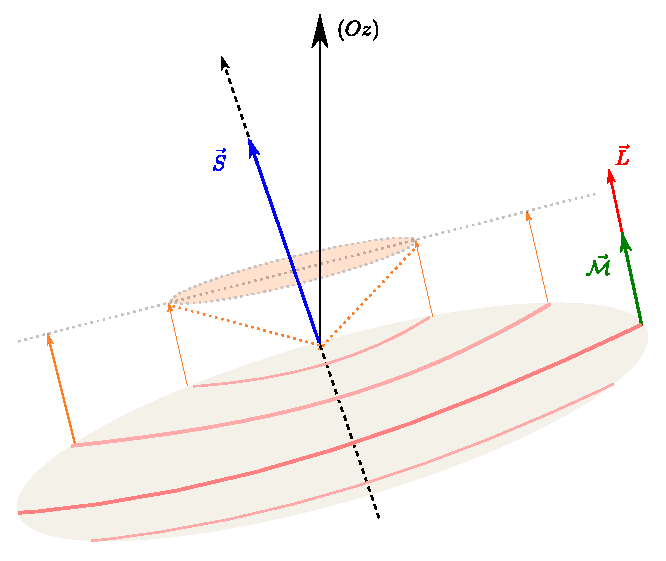
\includegraphics[width=0.8\columnwidth]{moments-cinetiques.pdf}
	\caption{\footnotesize{\textbf{Moments cinétiques des pales.} La pale (en marron clair) fait un angle avec la verticale (représentée par l'axe $(Oz)$), marque de la charge électrique. Le moment cinétique orbital $\vec{L}$ est perpendiculaire à la pale, tandis que le moment cinétique magnétique, assimilé au moment magnétique, en vert, lui est colinéaire. En orange, le flux à un endroit donné, dépend donc du rayon. Le spin est la densité de flux magnétique --~le vecteur de Poynting~--, donc la moyenne du flux sur la surface de la pale. Le flux, ainsi que le spin, est perpendiculaire à la surface. La figure n'est pas à l'échelle.}}
\end{figure}

Il faut bien se rappeler que la pale est une pale d'hélicoïde et qu'elle est mieux représentée comme suit (à l'épaisseur variable près):
\begin{center}
	\begin{tikzpicture}
		\def\a{0.2}
		\def\b{0.25}
		\begin{axis}[
			% Configuration de la vue et des axes
			view={120}{30},     % Angle de vue (azimut, élévation)
			width=\columnwidth, height=\columnwidth,
			axis lines=none,    % Masquer les axes pour un rendu plus propre
			xmin=-8, xmax=2,
			ymin=-7, ymax=5,
			zmin=-1, zmax=4,
			% Paramètres de rendu
			colormap/viridis,   % Palette de couleurs
			]
			% Tracé de l'hélicoïde
			\addplot3 [
			%surf,               % Type de tracé : surface
			mesh,               % fil de fer
			shader=interp,      % Lissage des couleurs
			opacity=0.9,        % Transparence avec surf
			domain=0:4*pi,      % Angle (rotation)
			domain y=0:2.5,     % Rayon (extension)
			samples=100,         % Nombre d'échantillons (précision)
			samples y=20,
			] (
			{(1 + (1/7)*x)*y*cos(deg(x))},    % x = r * cos(theta)
			{(1 + (1/7)*x)*y*sin(deg(x))},    % y = r * sin(theta)
			%{\b*(x + (1 - (1/7)*x) * y * 0.577)}   % si inclinaison (tan(30°)) 
			{\b*x}
			);
			% Optionnel : Tracer l'axe central
			%\addplot3 [black, thick, domain=-0.5:3*pi, samples=2, samples y=0] 
			%(0,0,{0.2*x});
			\draw[thin, -stealth] (axis cs:0,0,0) -- (axis cs:0,0,4) node[right] {$(0z)$};
		\end{axis}
	\end{tikzpicture}
\end{center}

La \MQ\ a pris le parti de considérer l'ensemble $\vec{S}+\vec{L}$ comme caractéristique de l'objet quantique. En réalité, le spin n'est pas totalement indépendant du moment cinétique magnétique intrinsèque, car il en est la somme sur 2 tours.

En effet, si l'on considère le nœud d'un point de vue énergétique, donc du travail, on a
\begin{equation*}
	\left\{
	\begin{split}
		\delta W &= P(t) dt = S dt \\
		\delta W &= \mathcal{M} d\theta
	\end{split}
	\right.
\end{equation*}
soit
\begin{equation*}
	S = \mathcal{M} \frac{d\theta}{dt} = \mathcal{M} \omega
\end{equation*}

Comme la vitesse de rotation du vorespace est la moitié de celui du neutrino, on obtient pour toute particule massique:
\begin{equation*}
	S = 2  \mathcal{M} \omega = 2 \frac{q_e}{2 m} = g \frac{q_e}{2 m}
\end{equation*}

%


Le \textit{facteur de Landé}, sorti un peu miraculeusement des équations de Dirac\cite{dirac1928quantum}, n'est en réalité que l'expression de la masse (donc du magnétisme) des particules que l'on mesure, c'est-à-dire des particules massiques.

Or la mesure du facteur de Landé montre qu'il n'est pas rigoureusement égal à 2, mais à 2 «plus un \R{2}{1000}». Le neutrino tourne donc un peu plus vite que deux fois la vitesse du vorespace. Si le facteur était de 2, ce serait un facteur fractal qui ne changerait pas les propriétés du vorespace, à savoir que le photon «traverse» le vorespace. Mais comme le facteur est très légèrement plus grand, la géométrie de la pale est très légèrement modifiée, et le photon ne peut plus «traverser» le nœud massique: il va buter dessus en transférant sa quantité de mouvement, créant l'interaction électromagnétisme.

Notez que l'on aurait pu directement intuiter ce résultat en disant tout simplement que le flux du vorespace est moitié moindre que celui du neutrino.

Notez enfin qu'en choisissant comme nombre quantique magnétique la projection de $\vec{L}$, la \MQ\ crée une confusion entre les genres. Certes, le moment cinétique orbital est relié au magnétisme, au sens où ce dernier est induit par la rotation, mais il aurait été bien plus heureux de nommer les nombres quantiques $m_l$ comme les projections de $\vec{\mathcal{M}}$. Il sera peut-être très difficile de remettre de l'ordre, à cause des habitudes. Mais la facilité de compréhension des domaines sous-jacents y gagnerait énormément\dots
\medskip

On peut désormais relier le facteur de Landé avec la constante de structure fine. Conformément aux calculs de la \MQ, le facteur de Landé correspond à l'agrandissement du cercle magnétique. C'est donc la partie du rayon excédentaire, et on retrouve donc classiquement le fait qu'il soit proportionnel à la constante de structure fine et que son facteur de proportion soit le tour d'un cercle complet:
\begin{equation*}
	g = \frac{\alpha}{2\pi}
\end{equation*} 

La masse, ou le magnétisme, induit donc une transformation plus subtile qu'un simple élargissement de la surface de la pale et de son épaisseur: elle induit un gonflement de l'épaisseur qui s'arrondit, un peu sur le modèle d'une chambre à air. Cet allongement, par rapport à l'épaisseur, est exactement le facteur de Landé, soit environ \R{2}{1000}.

Ce surplus rend le passage du photon impossible. Là où il passait en éfleurant le vorespace, la surépaisseur des nœuds massiques le bloque, induisant mécaniquement une interaction entre les photons et les nœuds de type $S_3$.

En outre, le rayon de la pale étant proportionnelle à la taille du nœud, on retrouve la loi logarithmique de la constante de structure fine \eqref{eq:structure-fine}.

Enfin, la vitesse apparente du neutrino, double du vorespace, ne doit pas cacher que seule la pale magnétique porte la vitesse réelle, soit le triple de la vitesse de celle du vorespace. Le surplus de vitesse s'applique par conséquence uniquement à cette pale, qui tourne donc un peu plus vite que 3. Pour l'électron, elle tourne à 3,002\,319\,304, soit un peu plus de 7\,~\% que la vitesse théorique. On retrouve bien le saut d'un peu plus de \R{7}{100} énoncé dans la loi fractale.
\medskip

Malheureusment, je n'ai pas été capable de calculer la valeur exacte de $g$ (ou de $\alpha$). Soit cela nécessite un esprit plus astucieux, soit cette constante est instrinsèque au plenum, et est donc la seule véritable constante fine de l'univers. Le modèle du Big Bang proposé plus bas peut faire pencher en faveur de cette hypothèse: il s'agirait du réglage exact correspondant à la quantité d'énergie nécesaire à la création du neutrino qui permet de développer l'interaction électromagnétisme dans l'univers.\footnote{Le fait que ce soit la seule «anomalie» rigoureusement non démontrable  chiffonne l'auteur. Toute la \PQ\ est structurellement mécanique et explicable, et cela devrait  aussi être  le cas ici. S'il est exact qu'il est impossible de calculer cette constante, alors elle serait effectivement le seul réglage fin de l'univers.}

\subsubsection{Les autres constantes de la physique}

Il faudrait prendre le temps de reconstruire toutes les constantes de
la physique, même si, à ce stade, on peut très bien tout reconstruire
mécaniquement avec celles déjà trouvées, car c'est \textit{grosso modo} ce que
fait la physique actuellement.

Il faut remarquer qu'une constante n'a aucun sens réel, c'est la
charge de Planck. C'est un simple effet de bord de l'extrapolation des
unités de Planck à toutes les caractéristiques de la physique: en
postulant une charge de Planck et en la définissant comme charge
élémentaire portée par une particule de Planck, une particule de la
taille de Planck. On a donc une impossibilité physique de représenter
une telle particule, sauf à l'associer à deux vorespaces ou à deux
neutrinos. La définition précédente renvoie au rayon de Schwarzschild,
c'est-à-dire à la masse maximale d'un objet, donc il s'agirait plutôt
d'un assemblage de neutrinos. Or, par définition, les neutrinos n'ont
pas de charge!

\section{Équivalence de la plénodynamique quantique avec la physique actuelle}

\subsection{Introduction} 

Il est nécessaire de s'assurer que la \PQ\  est compatible avec toute la
physique, si elle veut prétendre être une physique du tout. Elle s'est
construite sur la mécanique et sur la thermodynamique, ainsi que
sur l'électromagnétisme. Elle est déjà compatible avec ces théories.
Il faut toutefois encore passer l'épreuve des trois grandes théories
de la physique, à savoir les relativités restreinte et générale, ainsi que
la mécanique quantique.

\subsection{Relativité restreinte}

En ce qui concerne la relativité restreinte, c'est la partie la plus
facile, car la \PQ\ s'est construite justement en respectant les bases de
la relativité restreinte, à savoir un transfert d'information basé
sur la vitesse de la lumière comme vitesse maximale.

D'une certaine façon, la \PQ\ peut être vue comme le pendant réel de la
relativité restreinte, qui se trouve d'ordinaire être un cadre
général, valide partout. La \PQ\ incarne donc la relativité restreinte.

Il est aisé de retrouver le facteur de Lorentz dans une particule en
déplacement. Son évolution en chenille marque une différence entre le
début de son déplacement et la fin, que l'on peut triangulariser dans
un triangle rectangle qui permet alors d'extraire le facteur de
Lorentz.

Le temps ne se dilate pas à proprement dit, mais le temps de
recollement de la chenille s'allonge, car le chemin à parcourir est de
plus en plus grand.

De même, la tension dans la chenille augmente avec la vitesse, ce qui
donne en échange une augmentation de la masse, proportionnelle à cette
tension.

La \PQ\ est donc pleinement compatible avec la relativité restreinte:
on peut même dire que la \PQ\ \textbf{est} la relativité restreinte.

\subsection{Relativité générale}

Une part du travail a aussi déjà été réalisée dans le cadre de la
relativité générale. Ainsi, dans la théorie d'Einstein, une
masse courbe l'espace-temps et dans la \PQ, une masse agit sur le plenum
en lui imprimant une onde de cisaillement, le phonon de masse.

Là où Einstein montre que la lumière suit une géodésique de
l'espace-temps, le photon du plenum épouse le phonon de masse, en tant
que surfeur entropique. Il remonte les talwegs d'entropie, qui se
dirigent vers les masses.

Dans l'espace-temps d'Einstein, à proximité d'une masse, le temps
ralentit. Dans le plenum, le phonon de masse diminue les capacités de
transfert entropique, pénalisant le temps de transfert: plus le
phonon est massif, et plus le temps de transfert est pénalisé. La
masse agit bien comme un ralentisseur de temps autour d'elle.

Enfin, la relativité générale postule l'équivalence entre la masse
inerte et la masse grave. En \PQ, la masse grave est la masse du
vorespace, la tension qu'on peut appliquer à une turbine. La masse
inerte est celle engendrée par l'inertie de ce vorespace. Par
construction, elles sont identiques.

La \PQ\ est donc pleinement compatible avec la relativité générale.

\subsection{Mécanique quantique}

\subsubsection{Introduction}

On entre ici dans l'ultime étape. Si l'on peut prouver l'équivalence
entre la \PQ\ et la mécanique quantique, on aura alors uni les trois
grandes physiques et la \PQ\ sera définitivement compatible avec une
physique du tout.

On achèvera cette partie par la construction du modèle de l'atome
selon le point de vue de la \PQ, modèle qui permettra non seulement
de modéliser l'atome, mais aussi d'expliquer pourquoi il fonctionne
ainsi.

\subsubsection{La dualité onde-corpuscule}

Il va de soi que le phonon de masse et de charge (si besoin) autour
d'une particule constitue la fameuse onde des particules quantiques.
Elle n'est plus du tout mystérieuse, puisqu'il s'agit simplement de
l'interaction d'une masse, un corpuscule donc, avec le plenum.

Cette onde a néanmoins des propriétés intéressantes. C'est une onde
stationnaire heptagonale composite, au sens où elle est à la fois la
somme des ondes de chacun des sous-nœuds de la particule et de la
rotation de la particule elle-même.

Ainsi, dans le cadre de l'électron par exemple, composé de $2^{24}$ neutrinos, elle
est la composition de $2^{24}$~mini-ondes heptagonales mélangées à une onde
heptagonale de l'électron lui-même. \textit{Techniquement, l'onde n'est donc
pas composée d'une infinité d'ondes, mais d'un nombre fini.} Bien
entendu, la composition rend ce nombre «assez grand», ce qui rend
l'approximation «infinie» comme acceptable dans un premier temps.

À noter que l'onde définit entièrement la position de la particule. On
pourrait étudier seulement l'onde et rendre compte des
caractéristiques de la particule. De ce point de vue, l'onde
«pilote» bien la particule, ce qui était le point de vue de Louis de
Broglie.\cite{debroglie1924recherches}

Toutefois, c'est bien la particule qui donne naissance à l'onde et il
est plus juste de dire que \textit{la particule pilote l'onde}. Ce n'est donc
pas \textit{stricto sensu} une onde-pilote, mais plutôt une \textbf{particule-pilote},
si l'on veut garder la terminologie de Louis de Broglie.


À noter une différence majeure entre les deux théories: le
déterminisme est absolu en \PQ. Il «suffit» de calculer à quoi
ressemble l'onde pour déterminer à quoi ressemble la particule, et
vice-versa: l'une et l'autre étant en relation d'équivalence totale,
en bijection diraient les mathématiciens, il suffit de connaître l'une
pour tout savoir de l'autre.

Cette équivalence répond à la grande question quantique de ce que
représente exactement la fonction d'onde. L'école de Copenhague
affirme qu'elle contient en germes tout ce qu'il est possible de
connaître des propriétés de la particule quantique. C'est exact, au
sens où elle est engendrée par la particule quantique en question,
selon une relation déterministe qui tient compte de tous ses états. La
mécanique quantique part de cette fonction d'onde comme
référence de l'information, alors que la référence réelle est la
particule. En quelque sorte, la mécanique quantique suit un objet
éclairé par le soleil en suivant son ombre. Quand la mécanique
quantique mesure l'ombre, elle tourne alors son regard vers l'objet,
et affirme que l'ombre s'est transformée --~effondrée~-- en l'objet.
En réalité, \textit{la mesure quantique est juste un changement de point de
vue.}

Enfin, on a vu précédemment que la dualité onde-corpusculaire et la
quantification de l'impulsion entraînaient mécaniquement la formule de
de Broglie.

\subsubsection{Le cas du photon}

Le photon, notre surfeur entropique, pose un réel problème. Par
construction, il n'est qu'une onde. La dualité ne s'applique pas à son
cas, ce qui est pour le moins embêtant pour Albert Einstein qui a reçu
son prix Nobel après avoir expliqué le seuil de l'effet
photoélectrique par la présence de corpuscules de lumière!

En effet, la \PQ\ assume totalement changer le statut du photon en
physique. De même qu'elle a expliqué la nature réelle et la provenance
du photon, elle assume que le photon n'est qu'une onde pure.

La question qui se pose alors immédiatement est comment expliquer que
des milliers d'expériences de physique au cours de ces dernières
années mettent en évidence la double nature du photon? La réponse est
contenue dans la question: ce n'est pas la nature du photon que les
expériences mesurent, mais$\ldots$ les instruments eux-mêmes. Ainsi, quand
un photon se rapproche d'un détecteur physique, ce dernier, par sa composition
atomique, influe sur le plenum en créant un phonon de
masse, et même parfois de charge. Le photon, en tant que surfeur
phonique, «obéit» immédiatement au changement du plenum, créant
l'illusion qu'il est lui aussi doté d'une double-nature.

C'est peut-être la plus grosse révolution apportée par la \PQ: les
physiciens mesurent en réalité leurs instruments depuis des années
quand ils mettent en œuvre des photons!

\subsubsection{Le rôle de la mesure}

Voilà une transition toute trouvée pour examiner le rôle de la
mesure. Indépendamment du cas particulier du photon, qui est pourtant
l'acteur privilégié de la physique expérimentale actuelle, il faut se pencher
sur la notion de mesure en général.

En \MQ, la mesure impacte l'état du système, le réduisant à un état
propre, celui mesuré. La \MQ\ postule qu'un état quelconque de tous les
états superposés a été tiré au sort, selon un véritable hasard. Le
système est alors irrémédiablement réduit dans l'état mesuré.

On a vu ci-dessus qu'en réalité, la mesure quantique est un changement
de point de vue. Il n'y a pas d'écroulement de fonction d'onde, pour
la bonne raison que la nature révèle le réel et le réel est l'objet,
pas sa relation avec l'éther, même si cette relation peut
indirectement le définir. Il va de soi que lorsque les physiciens mesurent un
électron, c'est bien l'objet \node{$S_3(-1,1)$} qu'ils s'attendent à voir et à
mesurer, pas l'onde heptagonale qui l'entoure, même si cette dernière
n'est pas sans conséquence sur la mesure.

On a vu en effet que la mesure n'est pas sans impact au
niveau de la \PQ. En effet, les instruments de mesure, macroscopiques
par essence, ont un impact direct sur le plenum. \textit{Ils ne sont donc pas
neutres}. Pour expérimenter réellement, le physicien doit retirer le biais introduit par l'instrument lui-même.
Il sera compliqué de s'affranchir totalement de ce biais, quand on
mesure des objets de la taille quantique.

Reprenons par exemple le cas classique des interférences de l'électron
à travers deux fentes. L'électron possède une onde, c'est certain.
Elle peut très avantageusement interférer entre deux ouvertures,
forçant le passage de l'électron dans l'une plutôt que dans l'autre.

Mais quelle est la part du phonon de masse de chaque ouverture dans cette
histoire? Autour des deux ouvertures se créent deux couloirs de
phonon$\ldots$ Est-on certain que chaque ouverture est atomiquement
rigoureusement le miroir de l'autre (sinon, leur phonon de masse
risque de différer et, donc, de favoriser une mesure plutôt qu'une
autre)? De plus, il faut être certain de «taper pile au milieu des
fentes», car le lancer d'électron est déterministe en \PQ.
C'est-à-dire qu'en théorie, en lançant de façon identique les
électrons, ces derniers devraient suivre exactement la même trajectoire et
tous passer par le même trou. Bien entendu, il suffit de n'importe
quoi en cours de trajectoire pour changer un micro-paramètre et
changer le résultat final. Or l'air ambiant est rempli
d'interférences!

Bien entendu, la statistique vient comme bien souvent sauver l'expérience:
étant donné le grand nombre de paramètres incontrôlables, on peut
estimer raisonnable qu'ils s'annihilent statistiquement. On devrait donc retrouver
une justesse expérimentale via la statistique.

Quoi qu'il en soit, la question se pose de ce que l'on mesure
réellement aujourd'hui en physique$\ldots$ au moins au niveau quantique
quand on travaille sur les interférences.

Il va de soi que dès que le phonon de masse ou de charge peut avoir
une incidence dans une quelconque mesure, il faut en tenir compte, ne
serait-ce que pour prendre de la distance avec le résultat.

\subsubsection{L'intrication: le leurre du hasard}

Le fameux article EPR\cite{einstein1935can} d'Einstein, de Podolsky et de Rosen a lancé un
débat qui a pris fin récemment, mais que la \PQ\ se propose de relancer,
avec une conclusion inattendue. L'expérience postule que si la \MQ\ est
juste, alors il existe un état d'intrication entre deux particules et
que cet état viole la relativité restreinte, puisque l'information qui
circule entre les deux particules circulerait plus vite que la vitesse
de la lumière. L'expérience d'Aspect\cite{aspect1982experimental} a montré que cette affirmation
était vérifiée.

Pourtant, la \PQ\ affirme que le déterminisme existe et que, de fait,
l'intrication n'existe pas. Il s'agit simplement d'un effet de bord de la
théorie de la mécanique quantique, qui n'est pas la représentation la plus simple de
la réalité, mais une théorie plus complexe, comme évoquée par Poincaré\cite{poincare:1902:sh}.

La mécanique quantique emprunte donc un chemin indirect pour exprimer les
effets quantiques. Le chemin de la \PQ, plus direct, ne possède
pas les effets de bord de la mécanique quantique.

En effet, la mécanique quantique cache ce qu'elle ne connaît pas sous le
nom de hasard quantique. N'étant pas capable de calculer les
caractéristiques réelles d'une particule quantique, elle a élaboré
une technique divinatoire, excellente au demeurant, pour expliquer le
comportement des objets quantiques. Mais cette technique postule
l'idée d'un hasard irréductible, donc d'un indéterminisme structurel,
qui n'est pas le reflet de la réalité.

Prenons l'exemple de deux électrons d'un atome d'hélium. Ils sont
intriqués, au sens où chacun possède un spin opposé à l'autre. La \MQ\
affirme que seule la mesure lève cette indétermination. En réalité, il
n'y a pas d'indétermination: chaque électron possède réellement un
spin opposé à l'autre. Si vous en mesurez un, vous ne changez pas la
valeur de l'autre. L'intrication est une conséquence de la structure
(que l'on expliquera dans le modèle de l'atome), pas de la mesure.
L'intrication n'existe donc pas selon le point de vue de la
plénodynamique quantique. Vous pouvez déplacer deux objets intriqués
chacun à un bout de l'univers, en mesurer un, aucune information ne
circulera vers l'autre: les deux valeurs sont déterminées avant la
mesure.

Ainsi, l'article EPR qui supposait que la mécanique quantique fût
juste pour postuler la suite reste exact: c'est juste que l'hypothèse
de départ, la justesse de la \MQ, n'est pas conforme au réel. La
mécanique quantique utilise un hasard non réaliste qui a des
conséquences dans la mécanique quantique, pas dans la réalité.
L'intrication existe dans la mécanique quantique, pas dans la réalité,
car la mécanique quantique ne représente pas le réel, mais un moyen
mathématique et compliqué de décrire le réel. C'est une superbe illustration 
des dangers de l'utilisation des mathématiques pour décrire la physique, tel que l'énonçait de Broglie\cite{debroglie1976physique}.

Alors, comment se fait-il que l'expérience d'Aspect soit juste? Pour
exactement la même raison que les expériences sur les photons sont
justes: elles ne mesurent pas l'intrication \textit{in se}, mais l'interaction
des photons avec les instruments. Pour palier cette interférence des
capteurs, ici des lames, il faudrait mesurer les photons avec des
objets de la même nature que le photon lui-même. Sacré défi!

Quoi qu'il en soit, cela ne retire en rien à Alain Aspect d'avoir réalisé
cette expérience hors du commun.

\subsubsection{Le principe d'exclusion de Pauli}

Le principe d'exclusion de Pauli postule que deux fermions au même
endroit ne peuvent avoir des caractéristiques identiques. Ce principe
découle naturellement de la structure $S_3$ des fermions qui, pour être
ensemble, doivent avoir des caractéristiques physiques compatibles:
par exemple, pour assembler 2 $S_3$, il faut en retourner un, donc
inverser son spin, afin que les sens de vissage soient compatibles. Ce
principe est donc structurel dans la \PQ.

On verra dans le modèle de l'atome une raison plus fine de ce principe
qui découle en réalité de la minimisation de l'énergie des électrons dans les orbites atomiques.

\subsubsection{Théorème CPT}

La conservation CPT est structurellement conservée dans un nœud $S_3$
par la symétrie des 64 premiers états et des 64 suivants. L'inversion
de chiralité oblige à passer par tous les états intermédiaires. La
symétrie CPT est assurée par la structure de la turbine.

Quoi qu'il en soit et quels que soient les nœuds, la structure à 128
états est structurellement compatible avec la conservation CPT.

\subsubsection{Le principe d'indétermination d'Heisenberg}

La \PQ\ ne remet pas en cause le principe d'indétermination
d'Heisenberg. Ce dernier ne dépend en effet pas de la théorie
mathématique de la mécanique quantique: c'est un constat «évident»
que deux caractéristiques liées ne peuvent être mesurées en même temps,
les temps de mesure respectifs n'étant pas compatibles entre eux.

De plus, la quantification spatio-temporelle du plenum rend trivial le
principe d'indétermination.

\subsubsection{Conclusion sur la compatibilité}

La \PQ\ et la \MQ\ sont donc pleinement compatibles. La \PQ\ permet
simplement de corriger légèrement le tir de la \MQ, dont le hasard
intrinsèque a conduit à des conclusions parfois$\ldots$ hasardeuses. Le
déterminisme retrouve son plein droit dans le monde quantique qui n'a
plus rien de bizarre, les particules quantiques ayant retrouvé une
trajectoire déterminée.

\subsection{Le modèle atomique}

\subsubsection{Introduction}

Jusqu'à aujourd'hui, la physique a constaté que l'atome existait et en
a déduit un modèle basé sur des données purement expérimentales. C'est
un cas classique d'une «loi», extrapolée à partir de constatations
expérimentales\cite{poincare:1902:sh}. Si le modèle est juste, car il colle à l'expérience,
il ne propose en revanche aucune explication du «pourquoi» les choses
fonctionnent ainsi, et notamment, il n'apporte aucune réponse à la
\textbf{grande question}: «pourquoi l'électron ne tombe-t-il pas sur le
noyau?», question qui pourrait se poser via sa version contraposée:
«pourquoi l'électron tourne-t-il sans dépenser d'énergie?» La \PQ\
se propose de résoudre cette énigme et d'apporter pour la première
fois une réponse consistante.

Sans entrer dans les détails, l'idée générale de la construction de l'atome est de
trouver un état stable naturel à partir des particules élémentaires.
Ces dernières ne sont qu'une étape avant la stabilisation finale, qui
est l'atome. La stabilisation dans le plenum est toujours assurée par
un nœud auto-similaire à $S_3$, donc, sans surprise, on va retrouver cette
structure dans l'atome. L'électron et le noyau vont jouer le rôle des
hélices et «s'emmêler» pour former un nœud de type $S_3$. Bien
entendu, à ce stade avancé des particules, la fusion ne sera physiquement 
plus possible, et le nœud $S_3$ sera fortement distendu:
l'électron et le noyau ne seront donc plus collés.

En revanche, cet espacement laisse de la place libre pour former un
enchevêtrement complexe de nœuds $S_3$ dont chaque nœud ajouté
correspondra à un atome du tableau de Mendeleïev. La nature a tant
besoin d'épouser cette forme de nœud $S_3$ pour se stabiliser que
l'ensemble des couches électroniques forme lui-même un nœud de type
$S_3$!

Alors, prêt pour le voyage au cœur de l'atome? C'est parti$\ldots$

\subsubsection{Les bases du noyau atomique}

On a vu que les quarks, pour converger vers une structure stable de
nœud de type $S_3$, s'associaient par triplet pour former un neutron et un
proton.

Techniquement, la nature aurait pu s'arrêter là, mais la présence
d'électrons va forcer les neutrons et les protons à trouver une forme
commune de nœud pour encore plus de stabilité.

On pourrait s'étonner d'inclure le neutron dans le problème, car une
bête association proton-électron suffit par exemple à assurer la
neutralité électrique. Mais cette association seule ne permet pas de
dérouler tout l'ensemble des nœuds possibles, seulement de l'initier. Le neutron va
assurer la «glue» permettant de construire cet ensemble. Pour le
moment, admettons la nécessité d'inclure le neutron pour construire le
noyau et étudions ce qu'il se passe.

La seule forme stable pour un proton et un neutron est de former un
nœud de type $S_3$, donc un enroulement de trois quarks. C'est un modèle
légèrement hybride par rapport au modèle standard du plenum qui veut qu'il y ait
seulement une double hélice. Ici, on a une triple hélice et il est
raisonnable d'admettre que l'hélice double composée des mêmes quarks
joue un rôle unique, celui de la seconde hélice dans le modèle
standard (de la \PQ!) En effet, s'il y a trois hélices, l'objet obtenu n'est plus un
spineur. Un doute persiste sur laquelle des deux hélices va travailler de
concert avec l'autre. Il est plus «ockhamien» de choisir les quarks
identiques pour jouer un rôle similaire.

Le proton et le neutron sont donc techniquement des nœuds $S_3$,
c'est-à-dire des turbines, à l'instar des vorespaces du plenum. Pour
s'associer, ils doivent donc suivre les règles des turbines, et donc
permettre l'emboîtement des pas de vis. Un neutron et un proton
doivent donc se présenter tête-bêche, afin de tourner en sens
contraire, pour ne pas se repousser. L'aspect général forme donc un
tore. Le spin de l'ensemble vaut 0.

À noter que dans la nature, il s'agit d'un nœud peu stable, d'où la
nécessité de s'unir avec un tiers pour former un nœud plus stable.
On s'arrêtera là pour le moment afin de construire notre premier
modèle d'atome, car la structure elle-même du noyau méritera ensuite
une partie dédiée.

\subsubsection{Les bases du modèle atomique}

Prenons l'exemple de l'atome d'hydrogène pour commencer: sa
simplicité apparente va puissamment nous aider à comprendre la suite.
Jusqu'à aujourd'hui, la physique considère l'atome d'hydrogène comme composé
d'une charge positive, le proton, et d'une charge négative,
l'électron. C'est juste, mais seulement en apparence. 

En réalité, le
proton n'est pas la charge opposée de l'électron: on a vu qu'il
s'agit du positon, qui est un \node{$S_3(1,1)$}. Le proton, quant à lui,
possède la \textbf{charge apparente} du positon, mais sa répartition est
totalement différente: il est composé de 2 charges \Ru{+}{2}{3}{e} et d'une
charge \Ru{-}{1}{3}{e}. Si l'on comparait la «turbine protonique» à la «turbine
positonique», elles ne se ressembleraient pas du tout. La seconde est une
turbine inversée de l'électron, donc une vis conique à l'envers,
tournant dans le sens opposé de celui de l'électron, tandis que le proton ressemble sans doute
à une vis à deux goulots, un large bien au-dessous de sa moitié et un
plus petit, juste au dessus. Surtout, il y a une énorme différence:

\textit{Les deux hélices du proton tournent simultanément.}

Il s'ensuit que le modèle classique de l'atome d'hydrogène basée sur une
pure charge électrique négative et sur une pure charge électrique positive
est faux. La charge positive est composite: elle émet deux phonons
de charge correspondant à la charge \Ru{+}{2}{3}{e} et un phonon de charge
correspondant à la charge \Ru{-}{1}{3}{e}. Si les hélices \Ru{+}{2}{3}{e} fonctionnent de
concert, on peut réduire les deux premiers phonons à un seul double,
de \Ru{+}{4}{3}{e}.

Comme les hélices sont emmêlées, alors les phonons le sont aussi. Il y
a donc interférence et il se crée un champ phonique autour du noyau,
composition des ondes heptagonales précédentes, avec des pics à \Ru{+}{4}{3}{e},
des pics à \Ru{-}{1}{3}{e} et des pics à $e$. Bien sûr, il existe toutes les
combinaisons. Globalement, il va exister des zones pseudo-circulaires
autour du proton, dans lesquelles une charge sera privilégiée.

Quand l'électron arrive dans un tel champ, il est guidé par la
thermodynamique du plenum. Il suit donc les chemins de basse énergie,
c'est-à-dire les vallées de néguentropie. Lui a sa charge négative qui
ne change pas: c'est une vraie charge $-e$. Il va donc suivre un chemin
d'équilibre entre les talwegs de \Ru{+}{4}{3}{e} et les talwegs de \Ru{-}{1}{3}{e}.
C'est un chemin de basse énergie, qui n'en consomme donc aucune:
l'électron orbite sans effort.

En revanche, il passe devant des pics de charges et il est obligé de
s'adapter devant chacune des charges: \textit{il doit donc se retourner pour
présenter une opposition de charge qui le maintient naturellement dans
la vallée de basse énergie}. L'électron oscille, et son spin alterne
à chaque fois qu'il se présente devant une nouvelle charge, les charges étant
réparties uniformément autour de la trajectoire. L'électron oscille
donc régulièrement tout le long de sa trajectoire satellitaire.

On peut encore rendre hommage à la vision de de Broglie qui avait
proposé un modèle très proche d'oscillation de l'électron au cours de
sa trajectoire, en lui donnant une longueur d'onde spécifique.\cite{debroglie1956tentative} En
réalité, encore une fois, le modèle doit être retourné: c'est la
trajectoire qui impose l'oscillation, l'électron n'oscillant pas de
lui-même, en tout cas pas dans ce cas.

Que se passe-t-il quand on ajoute un neutron? L'atome d'hydrogène
devient du deutérium et le neutron épouse le proton selon le processus
évoqué précédemment. Encore une fois, la physique actuelle «voit»
une charge nulle dans le neutron, mais si c'était le cas, ce serait un
nœud \node{$S_3(0,1)$}, une masse pure, c'est-à-dire un neutrino. Le neutron est
composé de 2 charges négatives \Ru{-}{1}{3}{e} et d'une positive \Ru{+}{2}{3}{e}. Par un
raisonnement analogue au précédent, il se forme une double hélice
bâillonnée, dont les deux fonctionnent de concert, celles de même charge
étant synchronisées. Il faut ajouter au champ précédent un nouveau qui
est la superposition des deux phonons évoqués. Fort heureusement, c'est
un champs proche, qui change peu le champ en place. Il se contente de
«resserrer» très légèrement la trajectoire.

On peut mesurer cette différence par les énergies de ionisation, en
ajoutant le tritium, avec un neutron de plus:
\end{multicols}

\vspace*{-1cm}
\begin{center}
	\begin{longtblr}[
		%theme=widecaption 
		caption={\footnotesize{\textbf{Énergie de première ionisation des trois premiers atomes}}},
		label = {tblr:5-0-4},
		]{
			colspec={Q[c,m]  Q[c,m] Q[c,m] Q[c,m] },
			rowspec={Q[c,m]},
			row{odd}={bg=blue!10!white},
			row{1}={c,mode=text,fg=white,bg=pkcolor, cmd=\textbf}, %cmd=\textbf, blue!80!orange
			rowsep=2pt, colsep=3pt,
			vline{2-Y} = {1}{0.3pt,gray!50},
			vline{2-Y} = {2-Z}{0.3pt,gray!30},
			hline{Z} = {0.1pt,blue},
			% nombre de col début et fin qui apparaissent à chaque page
			% 1 pour le titre par exempel
			rowhead = 1, %rowfoot = 1, 
		}
		
	Isotope               &  Composition                  &  Énergie d'ionisation &    Écart/Protons seuls  \\
	Hydrogène (\ce{^1H}) H&    1 proton                   &       13,59844 eV     &             --          \\
	Deutérium (\ce{^2H}) D&  1 proton + 1 neutron         &       13,60215 eV     &      $+0,00371\,eV$     \\
	Tritium   (\ce{^3H}) T&  1 proton + 2 neutrons        &       13,60338 eV     &      $+0,00494\,eV$     \\
	\end{longtblr}
\end{center}


\begin{multicols}{2}
C'est une confirmation. La trajectoire ne change globalement pas et
subit un léger effet correctif, à chaque ajout de neutron.
\medskip

Que se passe-t-il désormais quand on ajoute un proton? L'atome
devient de l'hélium avec deux protons et un neutron. On verra dans la
partie suivante comment s'arrange le noyau pour valider cette
association. On admet seulement à ce stade que le neutron sépare les
deux protons de façon à les isoler l'un de l'autre, en évitant autant
que possible leur répulsion. Le double emboîtement proton + neutron
inversé + proton est mécaniquement stable.

D'un point de vue de la charge électrique, il s'ajoute donc au champ du
deutérium un second champ protonique. Comme il s'agit de champs
harmoniques, les conséquences ne sont pas catastrophiques: il se
construit un champ similaire au précédent, décalé dans un sens ou dans
l'autre. Les mesures de rayon atomique montrent que ce champ se décale en
réalité vers le noyau.

Pour l'équilibre électrique recherché, il est nécessaire d'ajouter un
second électron. Pour les mêmes raisons que précédemment, l'électron suit la
même trajectoire que le premier et orbite donc au même endroit. 

La
présence d'un premier électron est cependant perturbante pour deux raisons:

\begin{itemize}
	\item La première est qu'il est de même charge, donc les deux électrons se repoussent;
	\item La seconde est que le premier a créé une onde phonique et que le
	second va entrer dedans.
\end{itemize}

Étudions la première conséquence. Le second électron va chercher un
emplacement qui minimise l'énergie entre les deux, en raison de la
répulsion électrique.\textit{ Les deux électrons vont donc essayer de se
placer naturellement aux antipodes l'un de l'autre.}

La seconde conséquence est encore plus impactante. L'onde phonique,
«l'onde de de Broglie», créée par le passage du premier électron,
est une onde oscillante, qui se propage tout au long de la
trajectoire. Le second électron, même placé aux antipodes, a deux
choix: lutter contre cette onde ou surfer dessus. Comme il suit bien
entendu toujours la trajectoire de moindre effort énergétique, il va
se placer en opposition de phase. Les deux électrons vont alterner de
façon opposée: \textit{c'est l'explication topologique de la règle de Pauli.}
Attention, il faut bien comprendre qu'elle n'est valide que parce que
les électrons suivent la même trajectoire.

On va arrêter là le modèle pour le moment et retourner voir ce qu'il
se passe dans le noyau.

\subsubsection{Le modèle fin du noyau atomique}

Si on sait que s'ajoutent les neutrons et les protons dans le noyau, on
ne sait cependant pas comment ils se structurent physiquement. Le modèle qui domine
aujourd'hui est celui du modèle en couches du noyau, qui se contente de
structurer le noyau en couches, sur le modèle des électrons, sans
expliquer les relations physiques entre les objets.

Le problème à résoudre est de savoir comment répartir les neutrons et les
protons selon l'ordre atomique. Bien entendu, la première idée qui vient à l'esprit, et
c'est une bonne idée, est de séparer les protons par des neutrons,
afin d'assurer une isolation électrique, pour éviter un éclatement due
à la répulsion. C'est donc la règle de base:

\begin{mybox}[breakable,colback=blue!10, colbacktitle=pkcolor]{Postulat 13}
	Toute paire de protons du noyau atomique doit être reliée par un neutron.
\end{mybox}
\medskip

De plus, en «vissant» un proton dans un neutron inversé, on peut
«visser» de nouveau, en ajoutant une même paire à chaque fois.

On peut essayer plein de possibilités d'associations, mais rien ne ressemble
rapidement de près ou de loin au modèle du tableau périodique. Il faut
revenir à la racine de stabilité du plenum et penser que l'arrangement
va singer un nœud $S_3$, donc une spirale croissante. Mais la répulsion
inter-proton va obliger à «bricoler» la spirale en cours de
formation, afin d'ajouter des neutrons «isolants» supplémentaires,
pour stabiliser la structure, en raison des vis-à-vis protoniques
qui apparaissent.

Pour bien comprendre le modèle 3D, il suffit de le projeter en 2D.
Tout est résumé dans la figure \ref{fig:6-0}.

L'idée est d'associer un neutron au proton précédent en le
décalant de $2\pi/7$ afin de former peu à peu une spirale logarithmique,
propre à la géométrie du plenum. L'hydrogène initie la chaîne et c'est
le deutérium qui engage vraiment la spirale, en décalant son neutron.
Ensuite, l'hélium se forme par ajout d'un proton. Le vis-à-vis des
protons est suffisamment partiel et ne permet pas de contrer la
spirale naissante.

Par contre, l'atome suivant est impossible à construire par simple
ajout de proton. En effet, le proton du lithium serait alors en
vis-à-vis avec l'hydrogène, et la répulsion électrique
forcerait à ouvrir la spirale. Il est donc nécessaire d'introduire
simultanément un neutron avec le proton, qui va non seulement isoler
électriquement les deux protons concernés, mais aussi les relier
mécaniquement. La spirale est ainsi «vissée» et doit suivre le
chemin minimal d'énergie.

\begin{figure}[H]
	\centering
	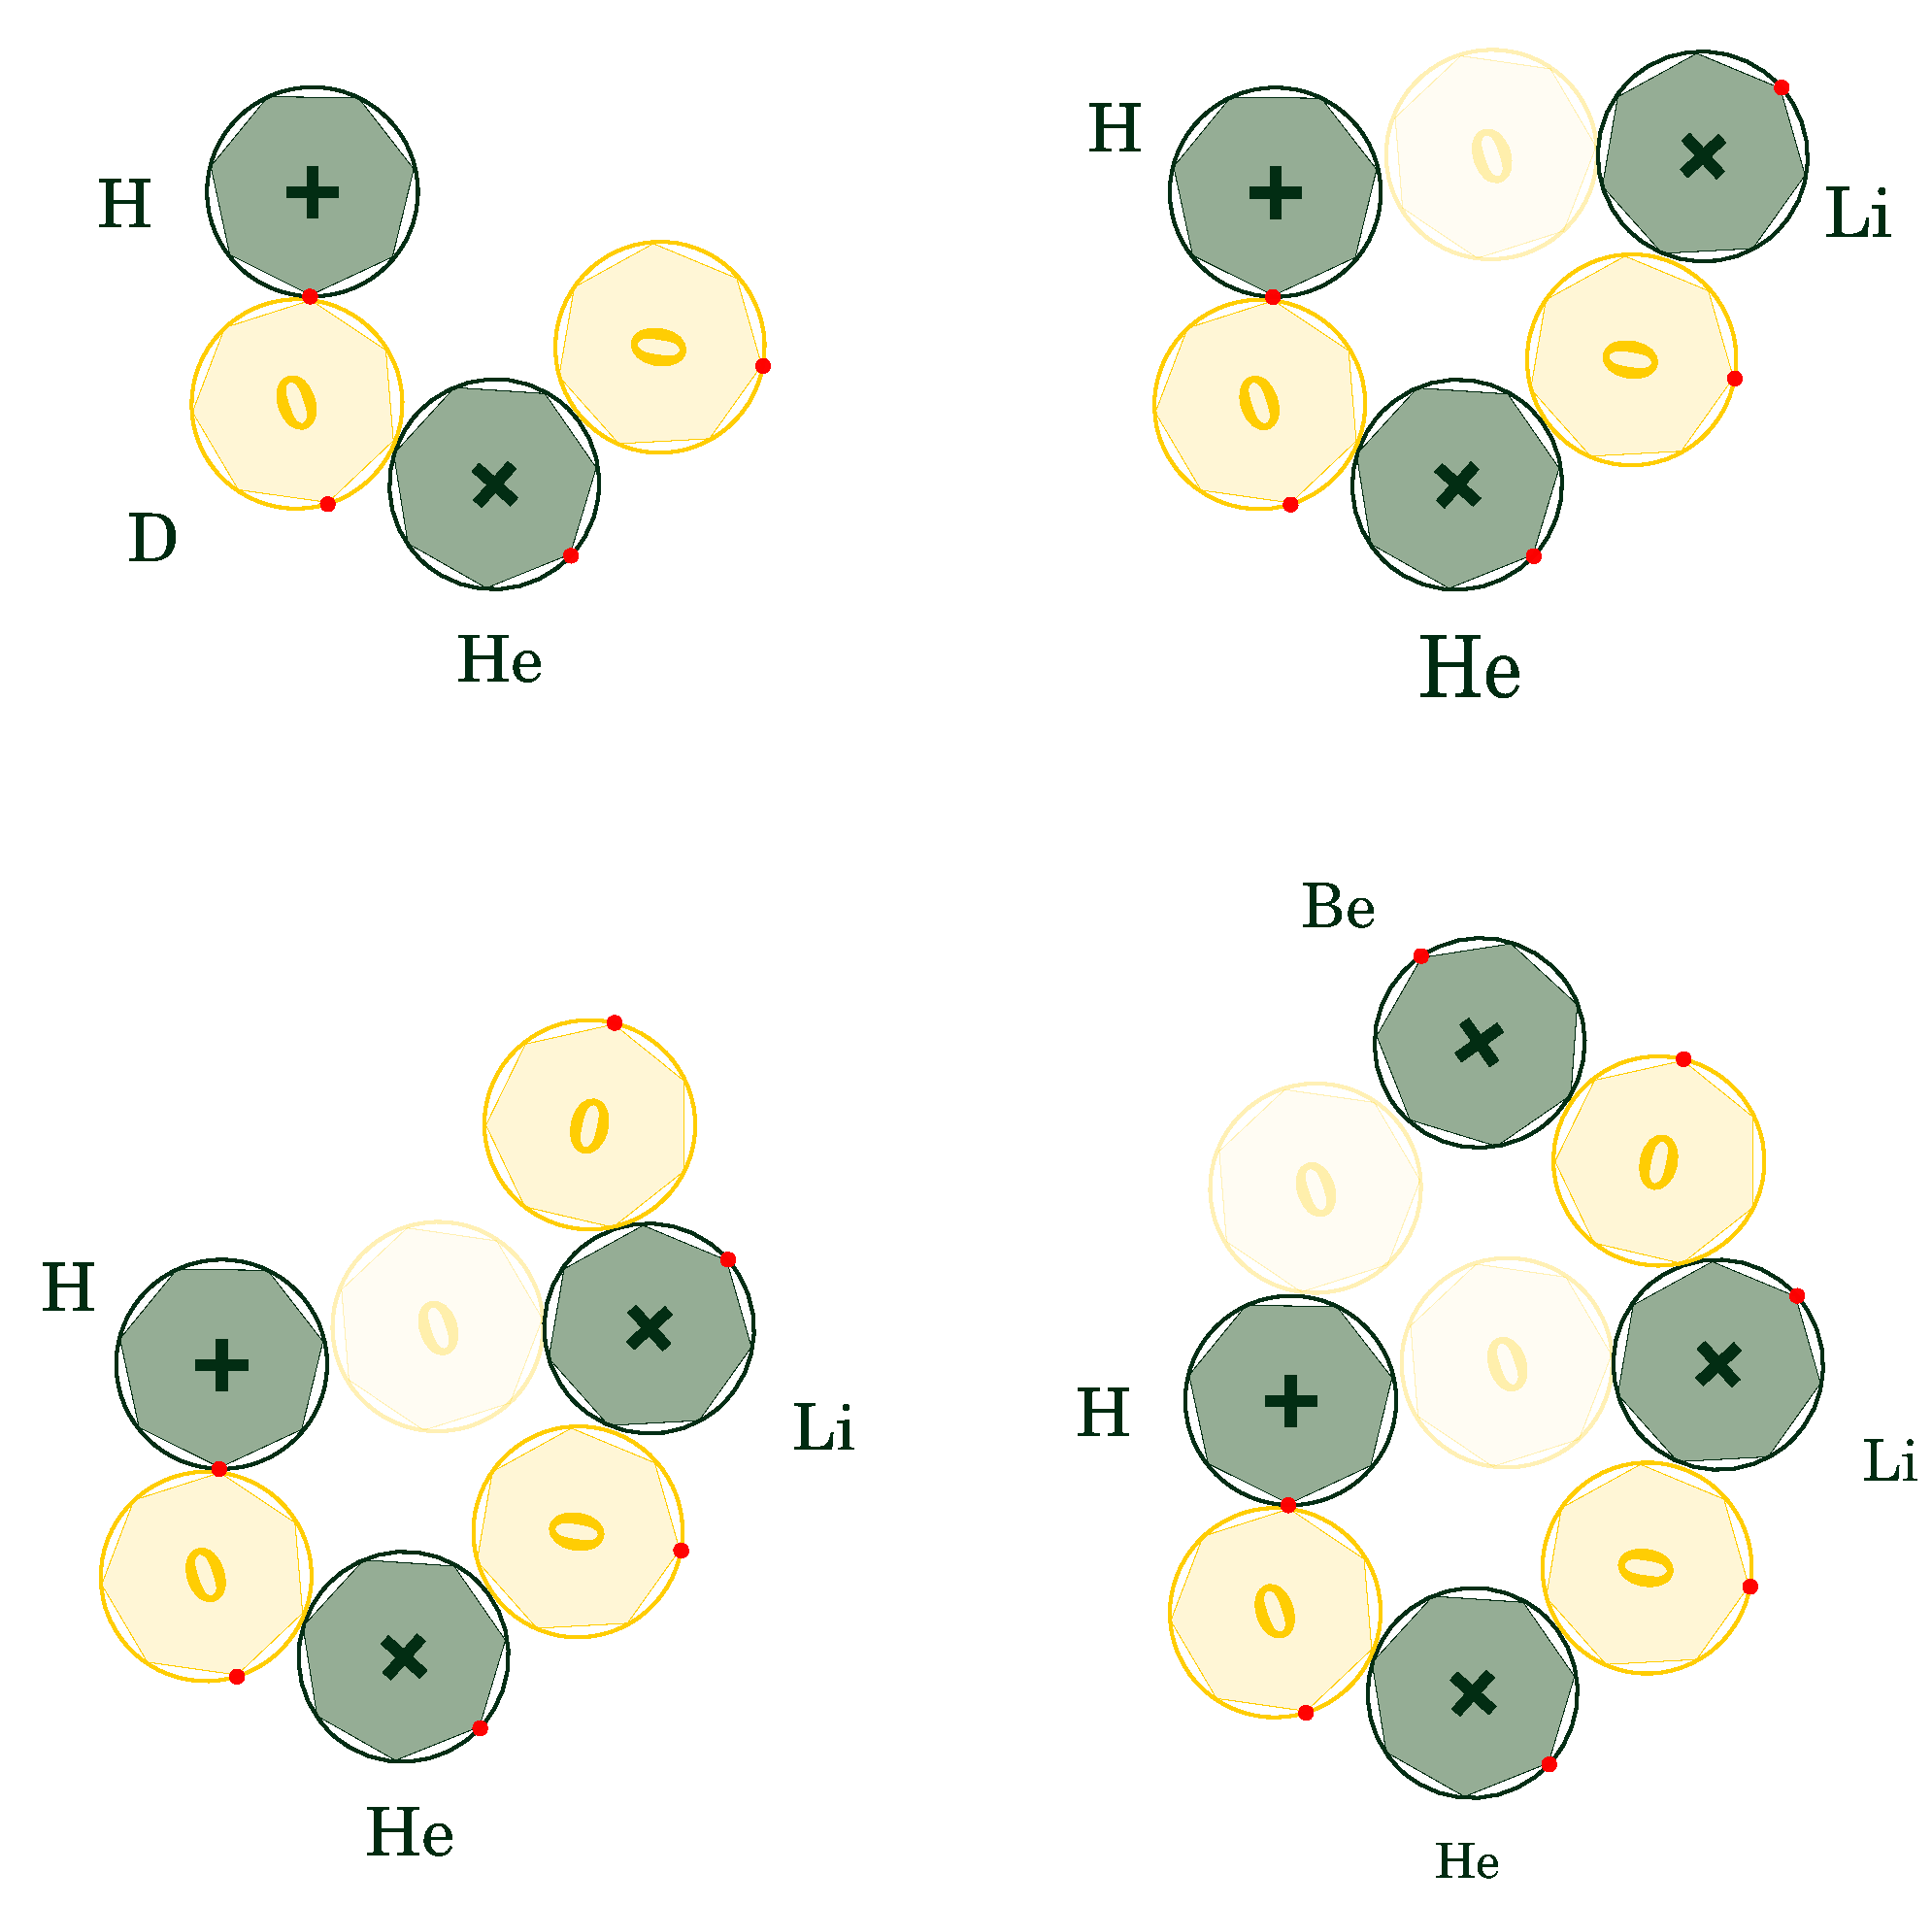
\includegraphics[width=0.8\columnwidth]{construction-noyaux-atomiques.pdf}
	\caption{\footnotesize{\textbf{Construction pas à pas des noyaux atomiques.} Le proton en vert est lié avec un neutron en jaune. L'association se fait par un décalage de $2\pi/7$ (que l'on peut suivre avec les points rouges), en créant une spirale. Pour éviter l'éclatement de la spirale par répulsion électrique, il est nécessaire de décaler l'emplacement d'un proton (en jaune clair) afin de lier deux protons non consécutifs. Le premier lien neutronique est entre le proton du lithium et le proton de l'hydrogène, le second entre le béryllium et l'hydrogène.}}
	\label{fig:6-0}
\end{figure}

On peut ainsi construire tout le tableau périodique. La figure
2D poussée jusqu'au calcium est la figure \ref{fig:7-0}.

On remarque que, même si la figure n'a pas été
exactement réalisée, l'oxygène et le calcium devant se
«rejoindre»:

\begin{itemize}
	\item les nombres magiques \cite{goeppert1949magic} apparaissent comme cycle d'achèvement du pas de
	vis;
	\item on résout au passage le saut du potassium qui nécessite deux
	neutrons, et rompt la série d'incréments de 1 dans le tableau
	périodique. En effet, il n'est pas possible topologiquement de
	joindre le potassium sans ajouter un neutron de liaison (en bleu) et
	il est aussi nécessaire de protéger le proton du potassium de celui
	de l'azote (en clair).
\end{itemize}

Le modèle du noyau est donc une spirale à 7 pas de vis.

\begin{figure}[H]
	\centering
	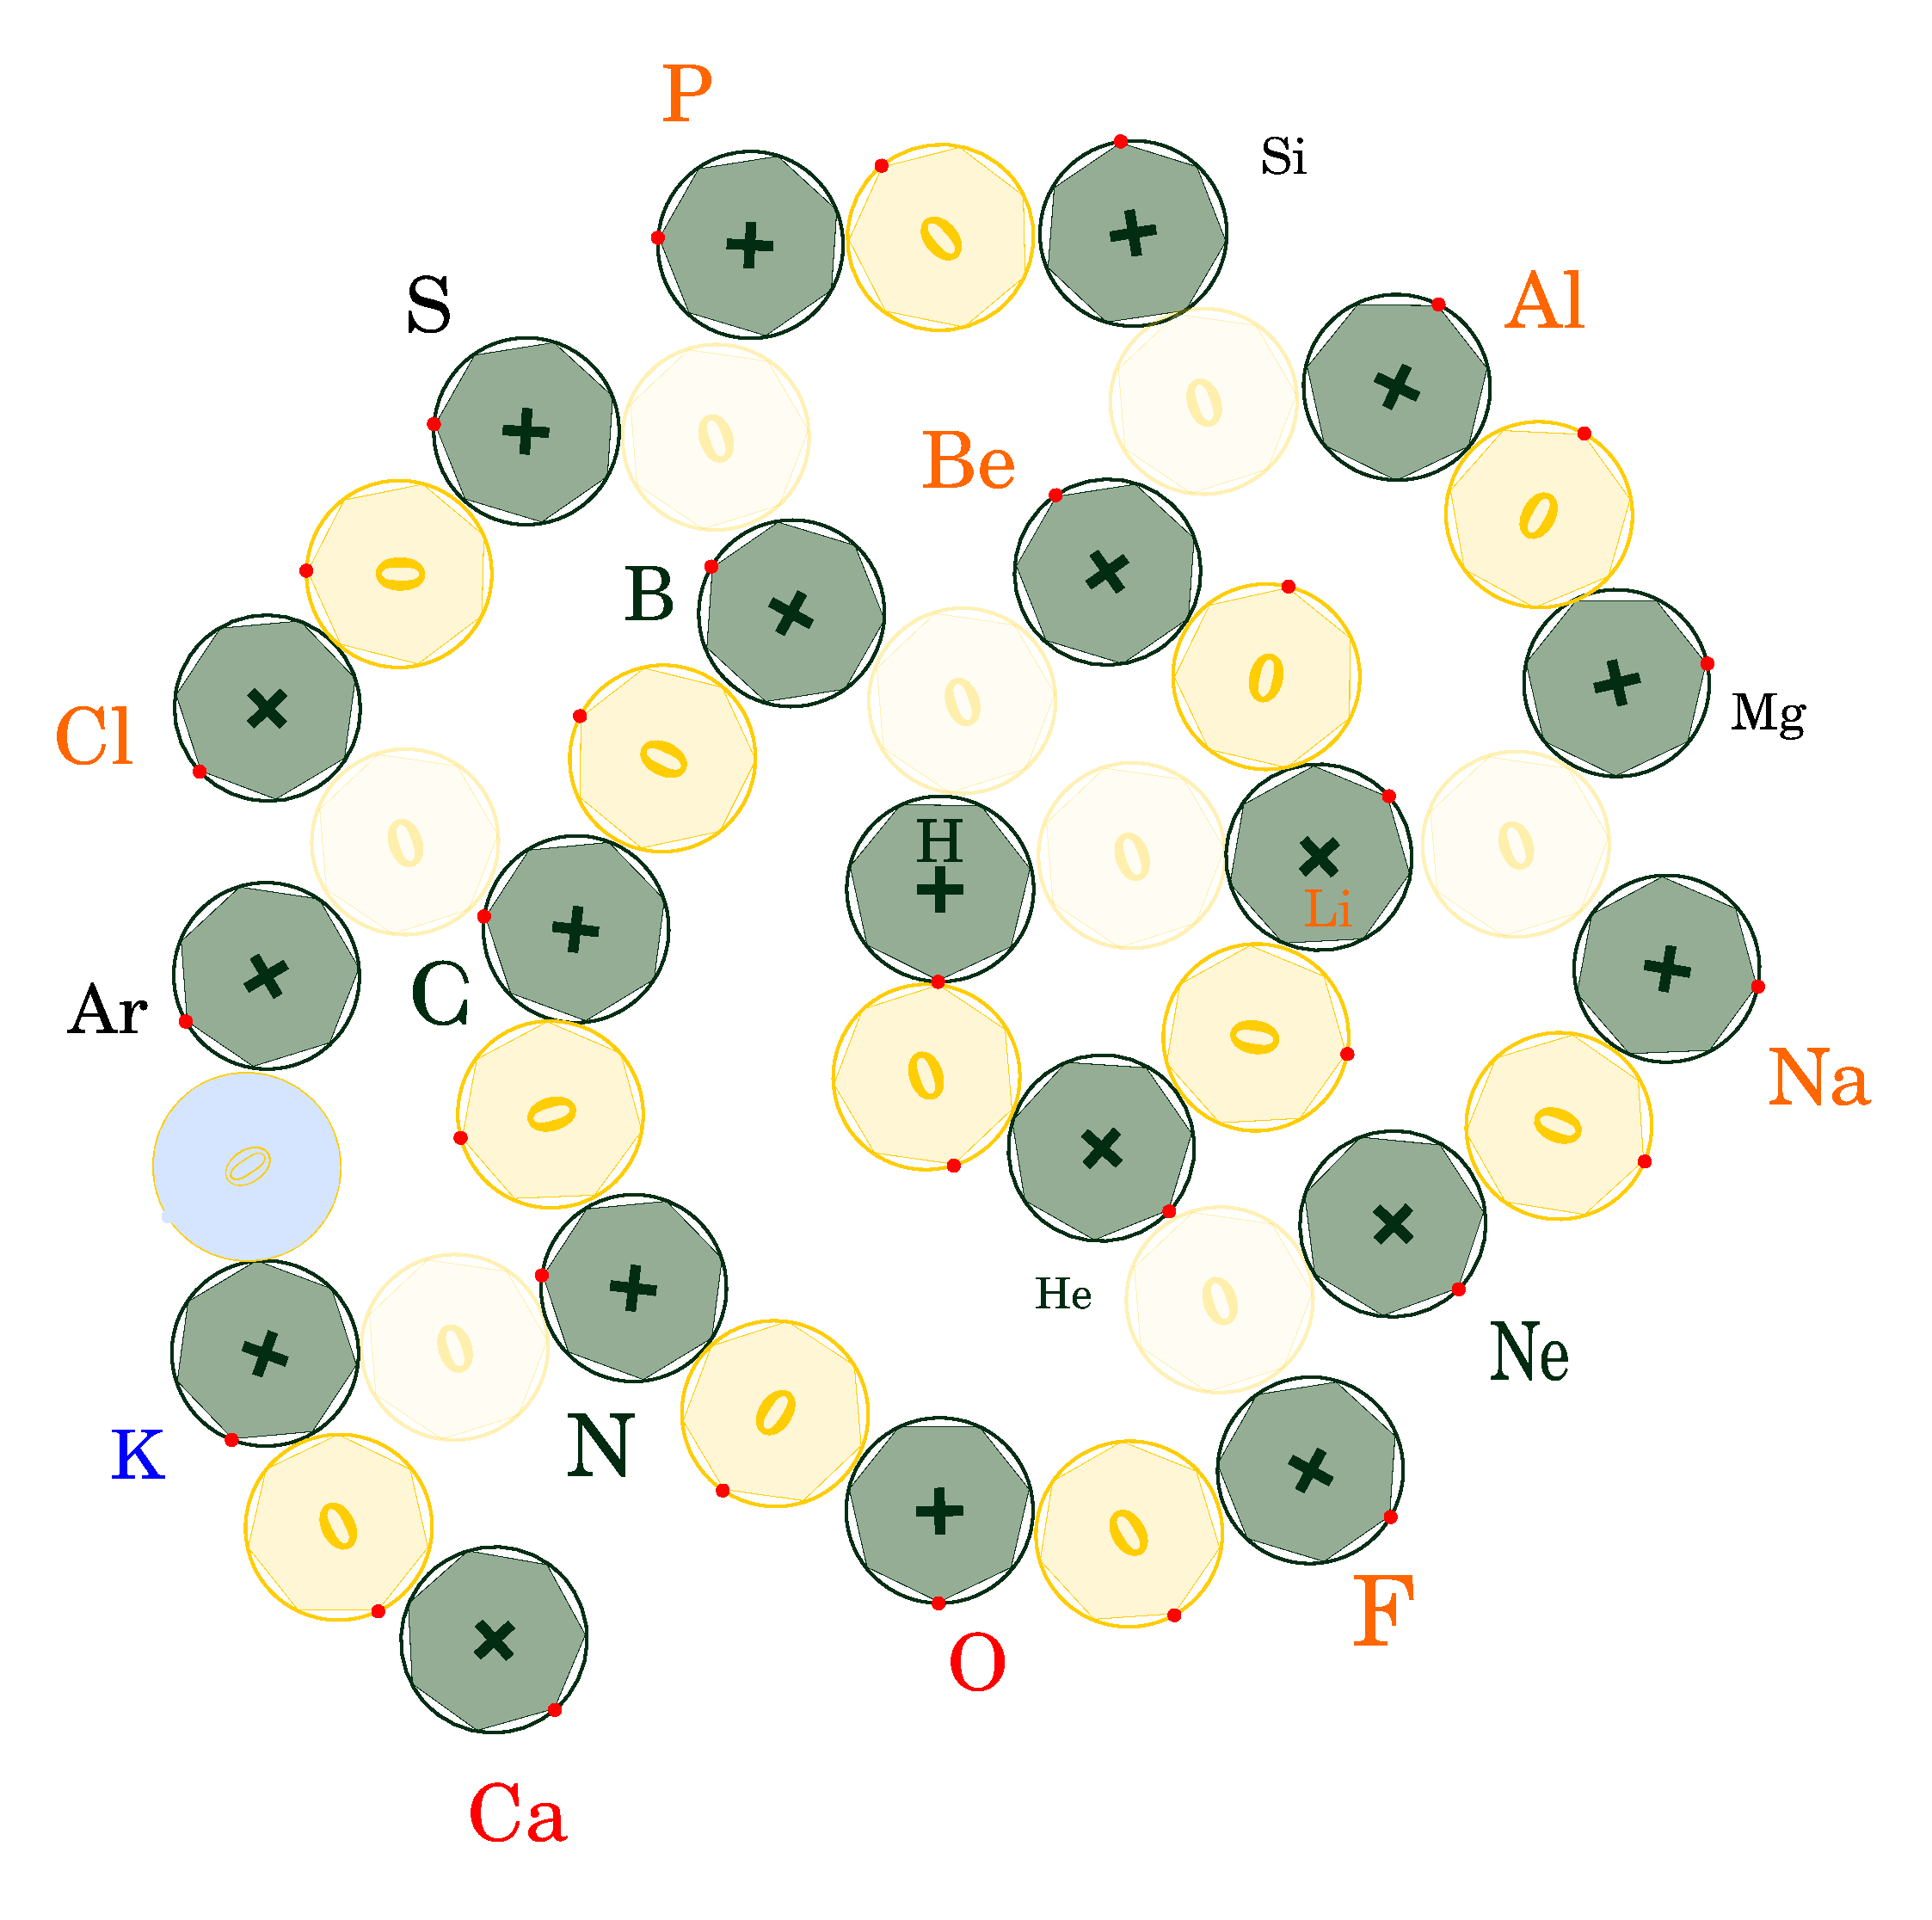
\includegraphics[width=0.8\columnwidth]{noyau-atomique-Calcium.pdf}
	\caption{\footnotesize{\textbf{Projection 2D d'un noyau de calcium.}
			Les points rouges permettent
			de suivre la rotation de la spirale (déphasage de $2\pi/7$), les neutrons
			clairs sont les neutrons à ajouter obligatoirement avec un proton pour
			équilibrer l'hélice (l'atome est alors marqué en orange). En rouge,
			les fins de cycle. La projection, ou plus sûrement mes talents
			perfectibles de dessinateur de spirale, ont faussé la figure:
			l'oxygène et le calcium devraient être alignés verticalement). }}
			\label{fig:7-0}
\end{figure}



\subsubsection{La force faible}

On a vu que la force forte était due à la structure d'emboîtement des
nœuds $S_3$ que sont les protons et les neutrons. Qu'en est-il de la
radioactivité, l'interaction faible?

Le modèle précédent du noyau permet d'imaginer ce qu'il se passe quand
il se met en rotation. Les éléments les plus hauts de la spirale, ceux
sur les pas de vis les plus élevés, ont mécaniquement une plus grande
vitesse de rotation, car ils sont sur un disque plus large.

Il existe un moment où la taille du disque, donc la vitesse des
couples de neutron-proton, est suffisante pour concurrencer la liaison
mécanique. Il suffit de trouver l'endroit où il y a peu de liens
neutroniques, ceux qui «vissent» les paires à la spirale.

Ce sont les paires en bout de l'hélice qui vont s'arracher. La raison
pour laquelle elles se séparent en doubles n'est pas forcément
claire sans calcul. Il est probable que l'énergie cinétique de la
double-paire soit exactement ce qu'il faut pour rompre un vissage
neutron-proton. C'est donc un noyau d'hélium 4 qui est éjecté, provoquant
le rayonnement $\alpha$.

\subsection{Les orbites électroniques}

Il faut conclure ce survol (trop rapide) du modèle atomique par un
petit mot sur les orbitales atomiques.

Le modèle de type $S_3$ pour le noyau impose un champ externe assez
complexe à calculer. Si l'on pouvait relativement l'intuiter sur les
deux premiers atomes, la complexité exponentielle rend en revanche vaine toute
explication «avec les mains» pour les suivantes.

Toutefois, à ce stade, en attendant une modélisation mathématique de la
\PQ, on peut extrapoler les résultats de la physique atomique pour les
introduire dans le modèle de la \PQ. On va donc récupérer les orbitales
de la mécanique quantique, en changeant leurs perspectives
de probabilité par une perspective de trajectoire.

La question qui se pose immédiatement est: pourquoi ne peut-on pas
mettre trois électrons dans une orbitale $s$? Tout simplement parce qu'il
n'y a pas assez de place pour réunir toutes les conditions en même
temps, à savoir équidistance des électrons et opposition de spin par
minimisation de l'énergie. L'introduction d'un troisième électron
obligerait un «placement à 120°» des trois électrons, ce qui
empêcherait un électron d'être dans un minimum d'énergie. Il
augmenterait la tension du phonon de «l'onde de de Broglie»,
bouleversant l'équilibre du système. Il est plus simple pour cet
électron de se placer dans un autre talweg de néguentropie, sur
l'orbite au-dessus.

Maintenant, rapprochons le nombre de couches électroniques de celui
des couches du noyau. Elles se répondent, évidemment, car l'association
couche électronique -- couche du noyau constitue en réalité une forme
dégénérée de nœud $S_3$, l'espacement entre les deux couches marquant la
dégénérescence.

Cette dégénérescence est en réalité intrinsèque à notre univers, «non
fini» comme on le verra dans le modèle du Big Bang. Elle indique
clairement la voie finale que prendra l'univers à sa fin: le dénouement
de tous les nœuds$\ldots$

Enfin, on peut ajouter que l'émission de photon de l'électron qui
change d'orbite trouve pleinement son emploi dans ce modèle. Chaque
orbite correspond à une vitesse donnée de rotation de l'électron, donc
à une exergie. Pour changer d'orbite, l'électron doit récupérer ou
céder les quanta d'énergie nécessaires à l'augmentation ou la
diminution de l'exergie. Si les orbitales sont assez proches,
l'électron semble sauter immédiatement de l'une à l'autre, alors qu'il
accélère (ou décélère) en réalité, pendant un temps multiple du nombre
de quanta utilisés. Il serait intéressant d'observer la trajectoire
réelle de l'électron et la manière dont il trouve un chemin entre les
talwegs de néguentropie «perpendiculaires» à l'orbite qu'il occupait
précédemment.

\subsection{Conclusion}

La \PQ\ est formellement compatible avec toutes les physiques, en résolvant
au passage quantité de problématiques physiques, comme le fonctionnement réel
de l'atome, la nature du photon ou la «supercherie» de l'intrication
quantique. Il faudrait désormais formaliser son statut mathématique
pour compléter la théorie. La partie suivante se contentera d'en
donner un bref aperçu.

Quoi qu'il en soit, la \PQ\ est à ce stade une théorie physique du tout.

\section{Formalisme mathématique de la plénodynamique quantique}

\subsection{Introduction}

Pour être exaustive, la \PQ\ doit également adopter un formalisme rigoureux. L'approche qualitive précédente a au moins le
mérite d'exprimer en mots et en images simples, et concrètes, le
formalisme mathématique sous-jacent qui est, lui, beaucoup moins
évident.

Toutefois, et par chance, ce formalisme est déjà connu et a été mis en œuvre
maintes fois pour donner du corps à toutes les théories physiques.
C'est une des raisons pour lesquelle il ne sera pas développé outre mesure. La
seconde raison est que l'auteur est trop faible en mathématiques pour
le faire en un temps raisonnable.

\subsection{Les bases mathématiques}

L'espace de la \PQ\ est celui de l'algèbre de Clifford $Cℓ_{7,0}(\mathbb{R})$,
c'est-à-dire un espace euclidien de dimension 7. Il engendre une série
de sous-algèbres de dimension 1 à 7 qui seront les bases des nœuds de la
\PQ.

$Cℓ_{7,0}(\mathbb{R})$ seule ne suffit pas pour définir la \PQ: il faut ajouter un
sens de rotation, une vitesse de rotation, vitesse qui sera le support
de l'énergie et une dimension (norme) contrainte. C'est ce quatuor qui
forme le modèle mathématique de la \PQ.

À cela doit s'ajouter le principe de fractalité reposant sur les
sous-algèbres de $Cℓ_{7,0}(\mathbb{R})$.

À noter que la contrainte spatiale ne change pas l'algèbre $Cℓ_{7,0}(\mathbb{R})$
\textit{stricto sensu}, qui reste une algèbre $Cℓ_{7,0}(\mathbb{R})$ à «rayon constant».

Enfin, les sous-algèbres de $Cℓ_{7,0}(\mathbb{R})$ sont très «parlantes» pour la
physique, car elles sont déjà très utilisées pour définir et manipuler
les objets sous-jacents, à savoir les nœuds de la \PQ.

Ainsi, pour résumer brièvement, on a

\clearpage
\begin{center}
	\begin{longtblr}[
		%theme=widecaption 
		caption={\footnotesize{\textbf{Listes des spineurs de $Cℓ_{7,0}(\mathbb{R})$ en fonction de la dimension}}},
		label = {tblr:5-0-4},
		]{
			colspec={Q[c,m]  Q[5cm, c,m]},
			rowspec={Q[c,m]},
			row{odd}={bg=blue!10!white},
			row{1}={c,mode=text,fg=white,bg=pkcolor, cmd=\textbf}, %cmd=\textbf, blue!80!orange
			rowsep=2pt, colsep=3pt,
			vline{2-Y} = {1}{0.3pt,gray!50},
			vline{2-Y} = {2-Z}{0.3pt,gray!30},
			hline{Z} = {0.1pt,blue},
			% nombre de col début et fin qui apparaissent à chaque page
			% 1 pour le titre par exempel
			rowhead = 1, %rowfoot = 1, 
		}
		dimension   & type de spineur                      \\
		   2        & Dirac, Weyl, Majorana, Majorana–Weyl \\
		   3        & Dirac, Majorana \\ 
		   4        & Dirac, Weyl, Majorana \\
		   5        & Dirac, symplectique-Majorana \\
		   6        & Dirac, Weyl, symplectique-Majorana-Weyl \\
		   7        & Dirac, symplectique-Majorana \\
	\end{longtblr}
\end{center}

Il est donc probable que le neutrino soit un spineur de Majorana, (car le \node{$S_3(0,1)$} est sa propre anti-particule), et que l'électron soit un spineur de Dirac (car le \node{$S_3(-1,1)$} n'est pas sa propre anti-particule).

Il n'y a donc rien de «nouveau» d'un point de vue mathématique dans
la \PQ. La \PQ\ ne fait que réutiliser les concepts mathématiques
qu'utilise la physique depuis près d'un siècle. \cite{hestenes1966space, lounesto2001clifford}

\subsection{L'équation de propagation}

Toutes les mécaniques physiques ont leur équation de propagation et il
serait sympathique d'en fournir une à la \PQ.

Bien sûr, en théorie, il faudrait développer la partie précédente pour
la démontrer. Mais il est peut-être possible de la fournir, car il y a une
grande chance que le travail ait --~là aussi~-- déjà été effectué.

On cherche une équation la plus compatible possible avec celle de la
mécanique quantique, la physique qui est quand même la plus proche de
la \PQ. Il faut donc prendre l'équation de Schrödinger et la
«corriger» pour tenir compte de la réalité physique qu'elle ignore,
et que la mécanique quantique contourne avec sa vision probabiliste.

Cette correction doit tenir compte de la loi fractale du plenum: elle est donc
une correction logarithmique.

Or il se trouve que cette équation existe déjà: c'est celle du
\textbf{gausson}, un soliton qui a toutes les propriétés des nœuds du plenum.\cite{bialynicki1976gaussons,}

L'équation de propagation d'un nœud pourrait donc être, à une dimension

\begin{equation*}
 i \hbar {\frac {\partial \psi} {\partial t}}=-\frac {\hbar^2}{2m} \frac {\partial ^{2}\psi }{\partial x^{2}}-\alpha\ln |\psi |^{2}\psi
\end{equation*}

ou, à 3 dimensions:

\begin{equation*}
	i \hbar {\frac {\partial \psi} {\partial t}}=-\frac {\hbar^2}{2m} \nabla^2 \psi  -\alpha\ln |\psi |^{2}\psi
\end{equation*}

C'est bien entendu une équation non-linéaire, ce qui ne va pas du tout
arranger les calculs à venir!

En revanche, il est probable que $\alpha$ soit la constante de structure fine, ou l'un de ses multiples.

\subsection{Conclusion}

L'auteur n'ira pas plus loin pour le moment sur le plan mathématique.
Pour être honnête, il lui faudra de l'aide pour y arriver! Mais il
reste confiant, tant le socle sous-jacent est archi-pratiqué depuis des
décennies.

\section{Les défis de la science et la plénodynamique quantique}

\subsection{Introduction}

Il peut être plaisant, pour finir de valider le modèle de la \PQ, de
s'essayer à résoudre certains problèmes que rencontre la physique
actuelle. La \PQ\ en a déjà résolu un certain nombre au cours de cette
présentation. On va ajouter seulement trois problèmes, parmi les plus
emblématiques, faute de place et de temps dans cet article. Une version ultérieure pourrait en présenter d'autres.

\subsection{Le modèle du Big Bang}

\subsubsection{Introduction}

Le Big Bang est le casse-tête absolu de la physique, étant une sorte
de quadrature du cercle. Qui naît de quoi et comment? On va voir que
non seulement la \PQ\ résout le problème de façon élégante, mais que
sa résolution apporte un grand nombre de réponses connexes que se
pose l'astrophysique: c'est en quelque sorte le «bouquet final
cosmologique».

\subsubsection{Le modèle}

On a vu que la \PQ\ est fondée sur une loi fractale et que le photon est
issu d'une dimension inférieure. Il est donc pratiquement évident 
que le plenum n'est aussi qu'une étape fractale d'un déroulement à
l'échelle inférieure.

Si le plenum est une échelle intermédiaire d'une loi fractale qui suit
l'algèbre de Clifford de dimension 7, à rayon contraint, alors le plenum est
forcément l'étape~3 (c'est-à-dire $Cℓ_3(\mathbb{R})$). Il existe donc, toujours
à rayon contraint, une étape $Cℓ_2$, une étape $Cℓ_1$ et une étape $Cℓ_0$.

L'étape $Cℓ_0$ est celle du bi-vecteur de Clifford «pur». Il
«définit» un rayon délimité, l'espace actuel, et engage une rotation
vers la gauche à une vitesse correspondant à l'énergie totale de
l'univers actuel. Le mouvement lévogyre trouve sa confirmation par
observation de l'univers actuel: la fractalité ne change pas les
caractéristiques fondamentales d'un objet par passage à l'échelle.

D'un point de vue d'un observateur «extérieur», l'univers est un
point, dans lequel est concentrée toute l'énergie. C'est la singularité
initiale.

Très rapidement, au temps $T_1$, sans doute de l'ordre de $10^{-512}\,s$ (on
doit pouvoir le calculer de façon exacte en extrayant la loi normale
du système), se crée le premier nœud: un cercle contient deux
cercles, chacun d'eux contenant deux cercles, selon une profondeur de 7, tous
étant décalés de $2\pi/7$. Il y a donc en tout $2^8$~cercles.

L'énergie de rotation initiale s'applique toujours au système qui, en 7
tours de vis, «sature» totalement les capacités d'emmagasinement de
l'énergie de chacun des cercles. Le système n'a d'autre choix que de
changer d'échelle et de monter vers le nœud supérieur.

Juste avant la bascule, un observateur extérieur a vu passer le point
précédent d'un état fixe à un état oscillant (sur la dimension de
l'espace). Le point a oscillé 7 fois.

C'est désormais le temps $T_2$, sans doute autour de $10^{-128}\,s$. Le
processus fractal s'applique et chacun des cercles précédents n'a
d'autre choix que de grossir d'une dimension, toujours selon un
processus de pas de 7: il y a donc $2^{16}$ doubles cercles. Mais comme le
processus se trouve multiplié en dimensions, il y en a  $2^{16} \times 2^{16}$ soit
$2^{32}$. L'univers commence à se peupler, mais d'une quantité d'objets assez 
peu importante, en regard de sa taille.

L'énergie des $2^8$ cercles précédents se répartit dans les
proto-photons nouvellement créés, par conservation de l'énergie. Les
photons sont en rotation, mais sans déplacement: ils s'illuminent. La
lumière jaillit pour la première fois dans l'univers.

L'excès d'énergie initiale continue à se répandre. Toujours au centre
de l'univers, la rotation s'effectue et, en 7 pas, se répand dans tous
les proto-photons. Ils saturent en énergie et n'ont d'autre choix que
d'effectuer une transformation fractale pour évacuer le trop plein. Au
moment de la transformation, le proto-photon quitte son status de
photon et n'émet plus de lumière. La lumière de l'univers s'éteint.

Le même observateur, toujours s'il pouvait exister, a constaté avant
l'extinction des feux que l'espace est désormais plan et qu'il est
balayé par deux points synchronisés, chacun sur un axe.

C'est le temps de Planck, là où commence notre physique actuelle, et
surtout notre univers. La troisième dimension apparaît et l'équilibre
thermodynamique conduit à construire exactement le plenum.

Chacun des $2^{32}$ proto-photons donne naissance à $2^8$ vorespaces, soit
$2^{256}$ vorespaces. Mais comme il y a une dimension supplémentaire,
alors le nombre croit par $2^{256} \times 2^{256}$ soit $2^{512}$ vorespaces.

On peut d'ores et déjà ce stade calculer la taille de l'espace. En effet, on a
\begin{equation*}
L_{espace} = 2^{512} \times \R{1}{2} L_p = 1,08 \cdot 10^{119}\,m
\end{equation*}

On note que cette taille justifie que la masse du photon, environ
$10^{-57}\,eV/c²$ soit invisible, car non mesurable.

On note aussi que la rotation des vorespaces, et donc des
neutrinos, selon un sens unique lévogyre, confirme l'hypothèse du sens
de rotation initial.

Le processus fractal continue et le trop plein d'énergie se
«déverse», toujours au centre de l'univers.

La façon dont se visse l'énergie, toujours dans le sens lévogyre de
départ, est importante à comprendre. En $Cℓ_1$, elle se vissait selon un nœud $S_1$,
en $Cℓ_2$, selon un nœud $S_2$ et donc dans le plenum, selon un nœud $S_3$.
\medskip

Il y a, à ce stade, deux cas de figures:

\begin{itemize}
	\item soit l'énergie est suffisante pour pousser jusqu'au stade $Cℓ_4$;
	\item soit il n'y a pas assez d'énergie.
\end{itemize}
 

Si l'on était dans le cas 1, alors l'histoire serait déjà terminée
et l'on serait déjà à l'étape suivante, ce qui n'est visiblement pas le
cas. Même en faisant l'hypothèse (très hasardeuse) que le processus de
diffusion de l'énergie est très lent, plusieurs milliards d'années, il
ne serait pas possible de créer quoi que ce soit  d'autre dans ce modèle
qu'une production continue de neutrinos, saturant peu à peu le plenum.
Le simple fait que ce ne soit visiblement pas le cas invalide cette
hypothèse.

Il n'y a donc pas assez d'énergie pour boucler une étape fractale
supplémentaire : l'univers s'arrête définitivement à l'étape 3, celle
de notre univers.

Que se passe-t-il donc à $t_3$, c'est-à-dire au temps de Planck, $10^{-43}$
seconde après le début du processus de création de l'univers?

L'énergie précédente des photons s'est distribuée dans les vorespaces
pour leur donner leur énergie de masse $\omega_v$, l'énergie du système à
l'équilibre. L'exécédent d'énergie se «visse» au centre de l'univers,
toujours selon la même procédure, ici donc sous la forme d'un nœud
$S_3$.

Tous les vorespaces contenus dans ce nœud géant tournent à la même
vitesse, la vitesse maximale, soit celle d'un neutrino. C'est une
concentration gigantesque de neutrinos, et comme le vissage a vissé
aussi les vorespaces qui tournaient dans l'autre sens, il y a autant
de neutrinos que d'anti-neutrinos.

D'un seul coup, le vissage s'arrête. Tout ce que l'on peut en dire, c'est
qu'il s'est arrêté entre le coup de vis numéro 1 et le numéro 6, car
s'il avait atteint le 7, le plenum aurait été saturé et, par
fractalité, aurait basculé dans $Cℓ_4$. Comme la taille de l'univers
visible est très faible par rapport à la taille du plenum, on peut
légitimement supposer qu'il y a eu très peu de coups de vis et, même,
supposer qu'il n'y en a eu qu'un.

Quoi qu'il en soit, le nœud $S_3$ est brutalement lâché sans pression à
ce instant-là. C'est alors la fournaise du Big Bang. Les neutrinos les plus à
l'extérieur sont beaucoup plus rapides que ceux coincés près de l'axe
central. Ils subissent une force de coriolis: c'est la mystérieuse
\textbf{énergie noire.} Le nœud se détend donc, dans un mélange d'éloignement
et de refroidissement, chaque neutrino et antineutrino pouvant alors
fusionner ensemble selon le modèle évoqué dans la \PQ. Il
fait suffisamment chaud pour que tous les nœuds $S_1$ à $S_7$ se créent,
ces derniers accaparant toute la masse. Il y a profusion de photons et
de pseudo-particules.

Puis, la température se refroidit, détendant le nœud $S_7$, et
permettant de dérouler le processus inverse qui va mener aux
particules élémentaires de notre univers. On retrouve notre bon vieil
électron, bien qu'il soit brièvement apparu lors de l'étape précédente.

\subsubsection{L'avenir de l'univers}

On peut se poser la question du devenir de l'univers. Le processus de
refroidissement défait clairement les nœuds massiques du plenum. La
fameuse stabilité de l'électron n'est en fait qu'une stabilité
d'équilibre et il est à craindre que dans un avenir très lointain, où
la température sera beaucoup plus basse, l'électron se dénoue en un
nœud $S_2$, qui se dénouera lui-même en un nœud $S_1$, puis en un neutrino.

Le final de l'univers ressemble à une soupe neutritronique à l'équilibre où chaque
neutrino occupera la maille d'un cristal géant. Il est possible que si
leur nombre est assez faible par rapport au nombre de
vorespaces, les neutrinos se diluent tout simplement, augmentant d'une
fraction l'énergie la masse de chaque vorespace.

\subsubsection{L'astrophysique de l'univers}

L'univers visible est donc un nœud $S_3$ géant en déroulement. Il n'est
donc pas plat, et sa courbure varie selon une double-hélice. Il existe
un axe central, qui explique le fameux «axe du diable» où les objets célestes semblent
absents. La tension de Hubble vient du fait que,
d'un côté on mesure le fond diffus cosmolgique, proche de nous et, de
l'autre des astres, sans tenir compte de l'effet de rotation de
l'hélice de l'univers visible,  ce que des travaux récents postulent en donnant une rotation à l'univers\cite{lodha2024hubble}. Cette hypothèse n'est d'ailleurs pas récente, car elle est postulée dans le modèle de Gödel\cite{godel1949example}.

\subsubsection{Conclusion}

Pour la première fois est exposé un modèle qui tient compte de
l'instant zéro et des étapes précédant le temps de Planck. D'autre
part, de ce modèle émerge aussi une vision nouvelle du
fonctionnemement de notre univers et il devrait être possible, avec la
masse fantastique des données de relevés astronomiques, de confirmer
assez rapidement ce modèle.

\subsection{Le trou noir}

Le trou noir est une singularité issue du modèle de la gravité selon
la relativité générale. Comme l'espace-temps d'Einstein n'a pas
d'essence, son repliement mathématique converge fatalement vers un
point géométrique, sans dimension, obligeant la gravité à devenir
infinie.

La \PQ\ résout bien entendu cette singularité, preuve de la limite de la
relativité générale. Par gravité, on peut, dans le plenum, dénouer tous les
nœuds et converger vers une densité maximale, celle où tous les
vorespaces d'une zone sont des neutrinos\footnote{Rien n'empêche que le processus respecte scrupuleusement l'ordonnancement des particules, donc une soupe de neutrons, puis une soupe de quarks, avant de finir en soupe de neutrinos.}. La dimension de l'espace
reste bien entendu finie, ainsi que la valeur de la gravité.

Le trou noir peut d'ailleurs se modéliser comme un énorme neutrino,
imposant une onde heptagonale gigantesque et «aspirant» tous les
objets à sa portée. L'horizon du trou noir est donc sa surface. Les
objets aspirés ne disparaissent pas, et pour ceux qui ne sont pas
capables de se transformer en neutrinos, ils restent collés dans le sillage
du trou noir. Aucune entropie n'est bien entendu perdue.

La question se pose de l'avenir du trou noir dans l'univers, à la fin
des temps. Il y a deux modèles: le premier modélise le petit trou
noir. Il reste compact jusqu'à la fin des temps, créant une verrue
dans le plenum. Le second modèle s'occupe du gros trou noir. Sa masse
gigantesque crée une vitesse de rotation différente entre les
neutrinos du cœur et les neutrinos périphériques. Le trou noir finit
par éclater, comme dans le modèle du Big Bang. Mais il n'y a plus
d'anti-neutrinos, seulement des neutrinos et le processus de fusion
n'opère plus. Les neutrinos sont expulsés et vont errer à l'infini, en
créant un cristal de neutrinos. C'est l'équivalent de l'évaporation
des trous noirs de Hawking. \cite{hawking1975particle}

\subsection{La catastrophe du vide}

La catastrophe du vide est l'écart entre la faible valeur de
la densité de l'énergie du vide observée (dont la valeur est limitée par celle
de la constante cosmologique) et la grande valeur théorique de
l'énergie du point zéro suggérée par la théorie quantique des champs,
qui peut atteindre $10^{120}$.

Si l'on calcule l'énergie de la structure de l'univers, on trouve

\begin{equation*}
	\begin{split}
	E_{struct} &= m_v \cdot 2^{512} \\
	           &= 3.8 \cdot 10^{-3} \cdot 2^{512} \\
	           &= 5,1 \cdot 10^{151}\,eV/c^2
	\end{split}
\end{equation*}

La matière noire représenterait environ 27\,\%\ de la matière totale et la matière baryonique environ 5\,\%. C'est la seule matière disponible, donc la seule énergie à disposition. Le dernier consensus de mesure donne environ 0,05 atome par mètre cube de matière baryonique, qui ne représente que 20\,\%\ de la matière totale. On doit donc tourner autour de 0,25 atome/m³, atome étant à prendre au sens large, puisque cela inclut la matière noire, qui ne peut arriver au stade atomique.

Les relevés du satellite Planck (2018) donnent une densité du vide de
l'ordre de 3.3\,GeV/m³, soit pratiquement 3 protons par mètre cube. Cette mesure inclut l'énergie noire, qui représente environ 70\,\%\ du tout. Il reste environ 1\,GeV/c² pour la matière, soit moins d'un atome par mètre cube. 

Dans un mètre cube, il y a $(1/2L_p)^3$ vorespaces, soit $1,9 \cdot 10^{105}$
vorespaces. Cela fait une énergie de structure de $7,22 \cdot 10^{102}\,eV/c^2$, soit environ $7,22 \cdot 10^{111}\,eV/c^2$ en ajoutant le baryon moyen.

\subsection{Pourquoi des spirales partout?}

On retrouve partout dans l'univers, et sur Terre, à toutes les échelles, une omniprésence de spirales logarithmiques. Elle s'explique par la convergence fractale naturelle vers des nœuds stables, de type $S_3$. Voici quelques exemples:

\begin{figure}[H]
	%\captionsetup{width=5cm}
	\centering
	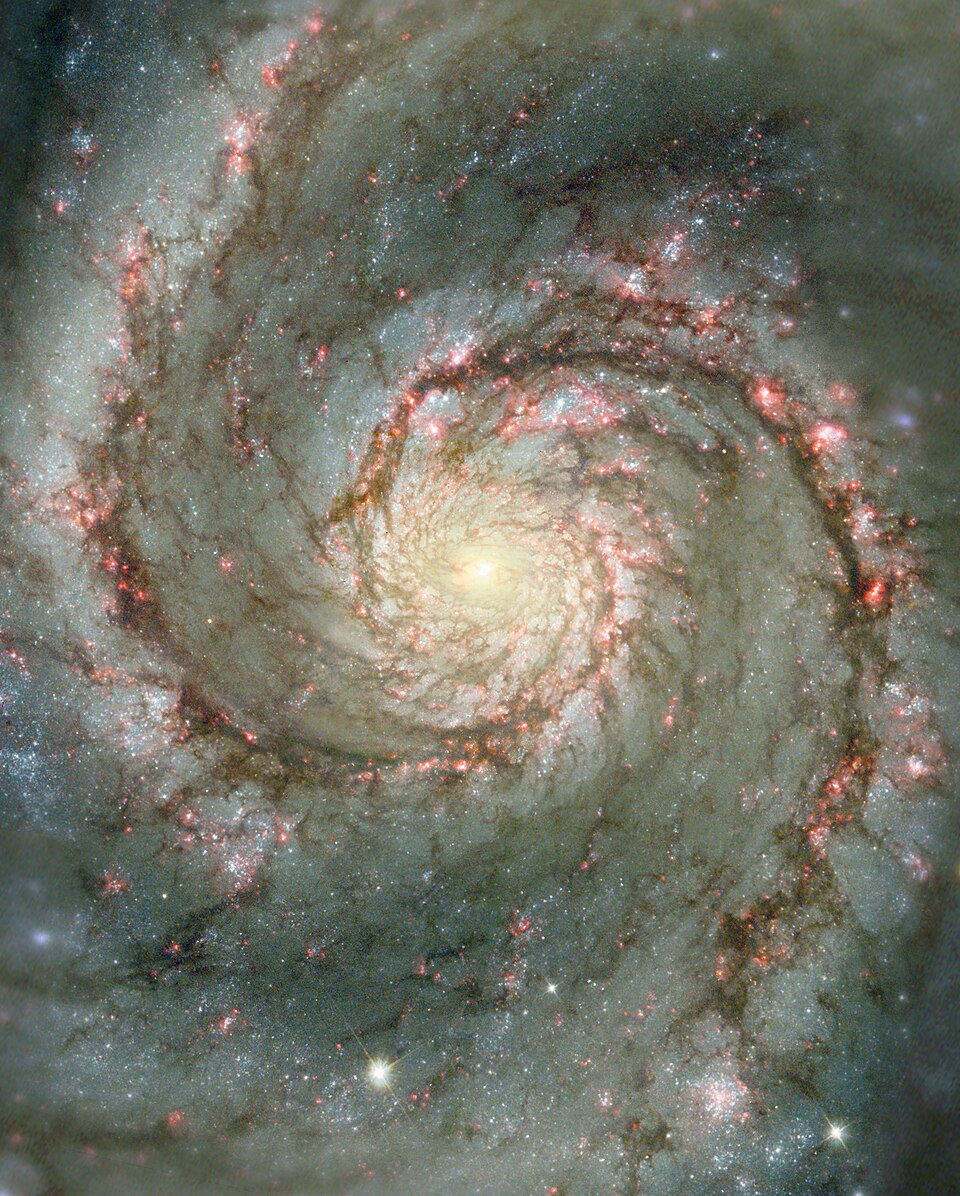
\includegraphics[width=0.7\columnwidth]{Whirpool_Galaxy-1.jpg}
	\caption{\footnotesize{\textbf{Galaxie M51.} Crédit: Wikipédia.}}
\end{figure}

\begin{figure}[H]
	%\captionsetup{width=5cm}
	\centering
	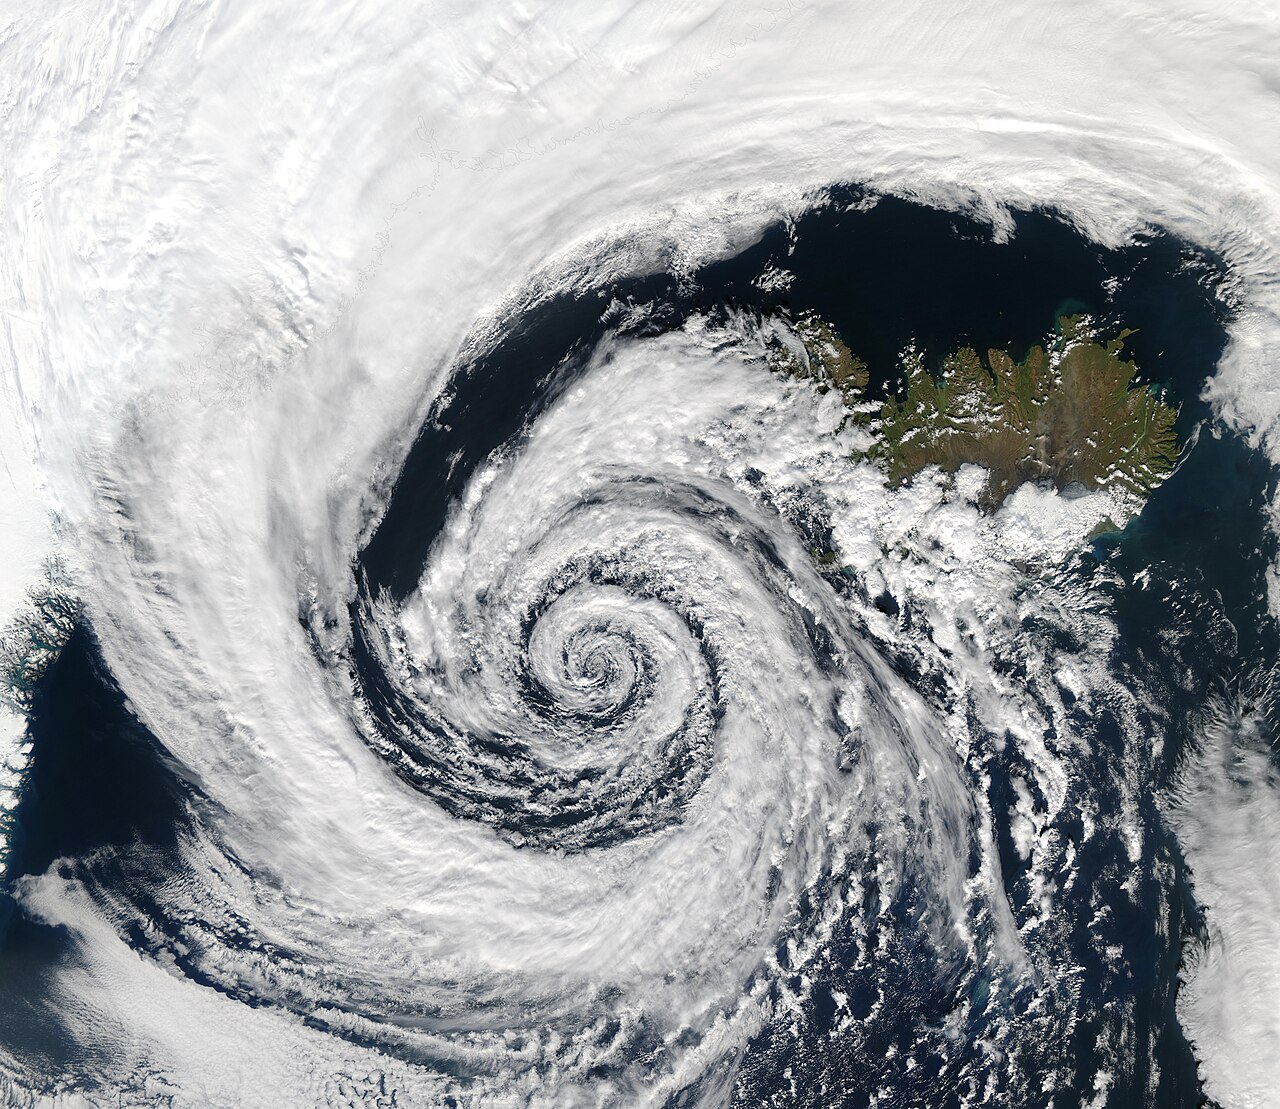
\includegraphics[width=0.8\columnwidth]{Low_pressure_system_over_Iceland-1.jpg}
	\caption{\footnotesize{\textbf{Cyclone polaire au large de l'Islande.} Crédit: Wikipédia}}
\end{figure}

\begin{figure}[H]
	%\captionsetup{width=5cm}
	\centering
	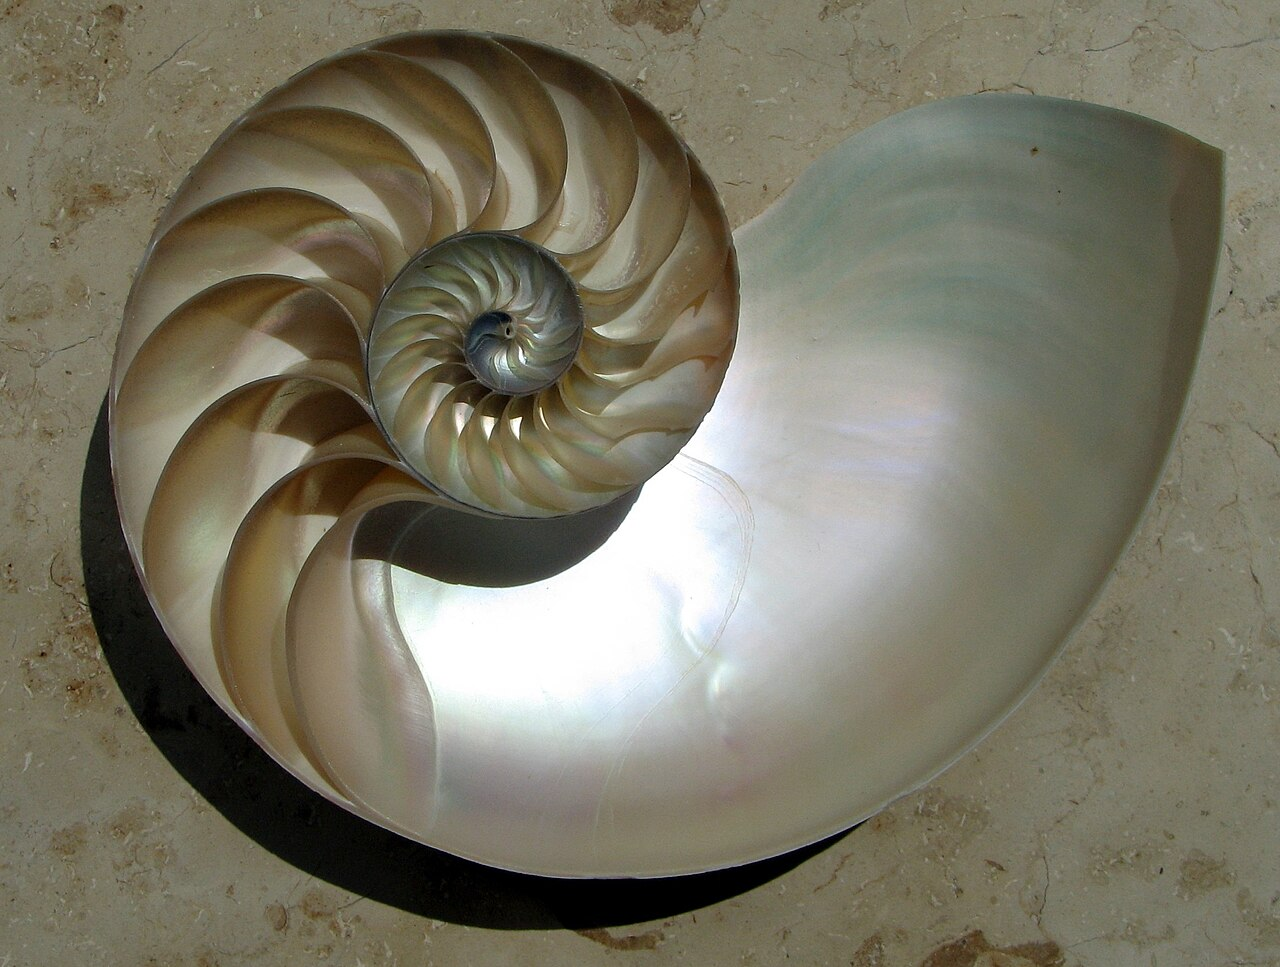
\includegraphics[width=0.9\columnwidth]{NautilusCutawayLogarithmicSpiral-1.jpg}
	\caption{\footnotesize{\textbf{Coupe sagittale d'une coquille de nautile.} Crédit: Wikipédia}}
\end{figure}

\begin{figure}[H]
	%\captionsetup{width=5cm}
	\centering
	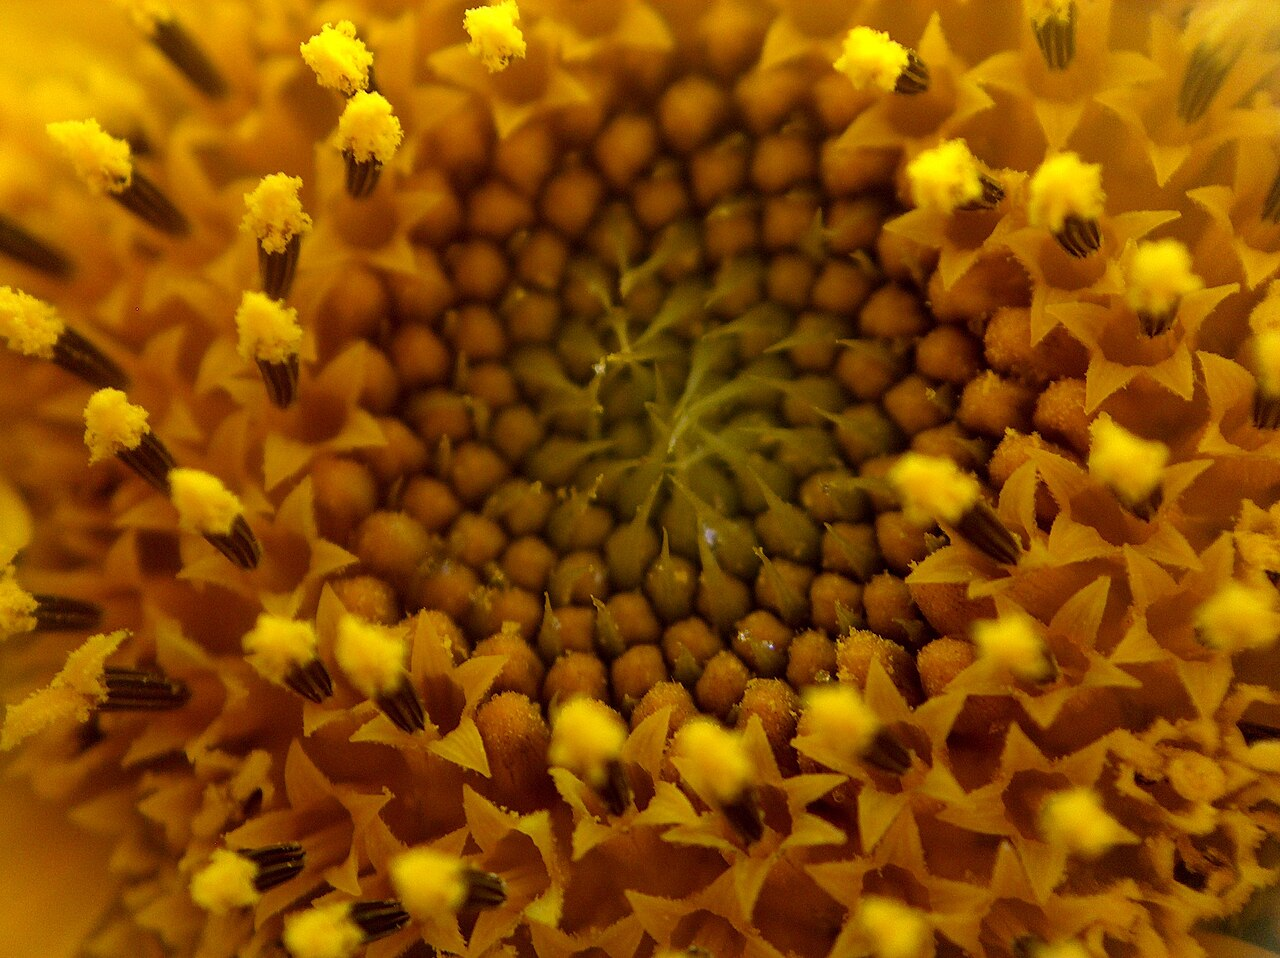
\includegraphics[width=0.9\columnwidth]{Close_up_Helianthus_annuus-2.jpg}
	\caption{\footnotesize{\textbf{Détail d'une fleur de tournesol.} Crédit: Wikipédia}}
\end{figure}

Il faudra bien entendu par la suite ajouter une représentation de l'électron, du neutrino ou des noyaux atomiques!

Mais la nature a beau tendre vers le nœud $S_3$, le «nœud admirable» de la \textit{spira mirabilis} de Bernouilli, elle n'y arrive pas toujours. Le modèle dévie parfois vers la spirale d'Archimède, dont le rayon est cette fois à incrément constant. On retrouve cette forme dans certaines plantes ou quelques phénomènes tourbillonnaires.

Quoi qu'il en soit, la nature est bien gérée par une loi fractale de type Fibonacci, de dimension 7, que l'on pourrait nommer une suite «heptanacci», avec une période de Pisano de 7. Quant à la «suite de Lucas», elle pourrait représenter les états d'énergie de chacun des nœuds. 

Il est donc normal de retrouver les spirales logarithmiques à toutes les échelles, preuve ultime du bien-fondé de la \PQ. 

\subsection{Pourquoi la vie?}

La question de la naissance de la vie, dans un article de physique
fondamentale, peut paraître au premier abord surprenante, voire saugrenue. Mais elle ne l'est qu'en
apparence. En effet, le modèle du Big Bang de la \PQ, et la \PQ\ en
générale, remet le déterminisme au centre de la physique. À une
condition donnée (une cause) existe une seule réponse possible (la
finalité).

Ainsi, la façon dont ont été réglées les conditions initiales de
l'univers, à savoir une rotation gauche, une énergie donnée, un rayon
contraint et 7 degrés de liberté, a engendré l'univers actuel sans qu'il
ne soit possible d'y changer quoi que ce soit. Ainsi, la matière est
née selon un ordre et cet ordre a donné une physique cosmologique dont
aucun paramètre ne relève du hasard.

Notre Terre est donc née de ce mouvement initial, comme une inévitable
conséquence de tout ce qui a précédé. Il est probable qu'un simple
changement de placement d'un atome à un temps cosmologique précédant
la création de la Terre aurait entraîné un univers assez différent:
c'est l'effet papillon à l'échelle cosmologique.

Il n'y a donc plus une trace de hasard dans le processus de création
qui a mené à la vie sur Terre.

Toutefois, il faut noter que le hasard s'arrête à l'aspect purement
mécanique du processus créatif: dès qu'un objet vivant est créé, ce
dernier ne suit plus une loi fractale, du moins est-il capable de s'en
éloigner dans son comportement particulier, même si le comportement
général procède toujours d'une fusion pour assurer la reproduction de
l'espèce \cite{queirosconde2003entropie}.
Le vivant n'a donc qu'un impact local sur le processus général à
l'échelle de l'univers.

Il faut aussi noter que le vivant est une rupture dans le processus
créatif. Dans notre univers, le nœud massique stable est de type $S_3$,
c'est-à-dire un nœud chiral. L'espèce humaine n'est pas chirale, comme
si le nœud exploitait ses capacités totales, une sorte de super
synthèse de tout le processus initial. De ce point de vue, il est
possible de voir l'espèce humaine comme le sommet, au sens de l'exploitation maximale, des capacités
créatives de l'univers.

\section{Métaphysique de la plénodynamique quantique}

Au \textsc{xvi}\ieme\ siècle, l'introduction par Newton des mathématiques dans la physique eut un effet de bord: la physique renonça à la métaphysique, puisque tout était mécanisme. Il suffisait de mettre le monde en équation pour l'expliquer.

Ce fut la mécanique quantique qui inversa la tendance quatre siècles plus tard, en introduisant
l'indéterminisme, à cause de sa base probabiliste. Si les
physiciens des anciens temps étaient tous formés à la métaphysique, ce
n'était pas --~et n'est toujours plus~-- le cas aujourd'hui. L'on eut depuis droit à
toute une série d'interprétations un peu bizarres où chacun y allait de
sa théorie, des univers multiples à l'intervention de la conscience de
l'observateur: tout semblait possible, à condition de renoncer à tout
esprit logique et à tout bon sens élémentaire.

La \PQ\ réintroduit de force un déterminisme absolu. Ce retour inattendu
du déterminisme a deux conséquences. La première est de déconstruire
toute la métaphysique se basant sur le «flou quantique» des
soixante-dix dernières années. La seconde pourrait être un formidable
retour en arrière de quatre siècles: tout est redevenu mécanique, fermez le
ban!

Mais est-ce vrai? Le modèle semble d'une grande robustesse et offre
pour la première fois une physique du tout cohérente, sans vrai trou.
On peut donc s'y fier.

\textit{Mais que dit-elle en substance?}

Qu'à l'origine du monde, il y a un bi-vecteur. Et qu'est-ce qu'un
bi-vecteur, si ce n'est un couple de deux objets liés si fort qu'ils sont
fusionnels? N'est-ce pas une définition très précise de la Sainte
Trinité? Deux personnes, le Père et le Fils, sont si liées qu'elles ont
donné naissance à une troisième personne, le Saint Esprit? \cite{aleteia_trinite_ref}

La coïncidense pourrait s'arrêter là. Mais que racontent les
Écritures? Dieu le Père, le vecteur de gauche, a soufflé (l'énergie)
et envoyé Son Fils, le Verbe, placé à Sa droite (le vecteur de
droite, qui lui passe donc devant en effectuant une rotation vers la
gauche), selon un processus effectué en sept étapes (\textit{cf}. la Genèse \cite{aelf_genese1}). Ne
sont-ce pas \textbf{exactement} les conditions initiales?

Poursuivons et observons ce que décrit le livre de la Genèse qui a été longtemps
décrié, à cause de la prétendue inversion de l'ordre des moments de création.
 Le Père commence par envoyer Son souffle à l'étape initiale
($Cℓ_0$), la terre et le ciel se créent, figuration des deux cercles
emboîtés ($Cℓ_1$), puis la lumière jaillit (le fameux «Fiat Lux») à $Cℓ_2$. La
Genèse est donc parfaitement en phase avec le modèle du Big Bang si,
bien entendu, on replace la notion de jour avec la notion de temps
fractal du modèle.

De plus, on peut voir un clin d'œil du roi David, dans le psaume 147,
verset 15, qui dit que «Il (le Seigneur) envoie sa parole sur la
terre: rapide, Son Verbe la parcourt.», \cite{aelf_psaume147} qui est une façon très poétique
de synthétiser le processus de la Création.

Notez que par construction fractale, tout est à l'image du bi-vecteur initial, donc à l'image de Dieu.

Enfin, la vie est une conséquence inévitable des conditions
initiales: il n'y a aucun hasard dans l'apparition de la vie. Si l'on associe Dieu au bi-vecteur de départ, alors la vie est bien une volonté initiale de Dieu qui a mis en place les conditions exactes de son apparition. 

Seule la vie engendre une rupture indéterministe dans le processus et cette
rupture est aussi expliquée dans les Écritures par le libre-arbitre. \cite{vatican_libre_arbitre}

La seule chose que la \PQ\ n'explique pas est l'âme. Mais si l'on se fie aux Écritures,
l'âme serait dans une autre dimension que notre univers, donc non
descriptible par cette théorie, ce qui rend raisonnable cette
affirmation. L'homme matériel serait le nœud le plus évolué de la Création et son âme un don de Dieu: il serait donc doublement et pleinement à l'image de Dieu (\textit{imago Dei}). 

Il serait cependant possible d'imaginer à quoi pourrait ressembler le monde invisible via la \PQ. En effet, dans les Écritures, il y a toujours une association entre le monde invisible et la lumière\cite{aleteia_lumiere_ref}. Le Christ est la Lumière du monde, les anges sont des êtres de lumière et Lucifer est lui-même l'être lumineux par excellence. D'autre part, la description d'un tunnel de lumière revient sans cesse dans les expériences de mort imminente. Le monde invisible est donc asssocié à la lumière et il a été créé avant le monde visible. Dans le processus de création via la \PQ, seuls deux états peuvent être associés à la lumière: $Cℓ_2$ et $Cℓ_5$, qui sont des ères photoniques. $Cℓ_2$ est l'ère pré-planckienne, avec peu d'éléments engendrés ($2^{32}$), ce qui semble insuffisant pour peupler le monde invisible de «myriades de myriades d'anges», expression biblique qui désigne une quantité astronomique. Seule l'ère $Cℓ_5$ semble être une bonne candidate à cet écrin de création. En effet, ses dimensions supérieures à $Cℓ_3$ et le nombre impressionnant d'objets constituant son «plenum» lui permettent d'engendrer --~probablement selon un processus identique à celui du nôtre, à savoir une énergie vissante non suffisante pour créer la bascule vers $Cℓ_6$~-- tous les êtres de lumière de la Création. Quant à savoir comment ils communiquent avec notre univers $Cℓ_3\dots$

Enfin, il «suffit» au bi-vecteur originel d'effectuer deux coups de vis pour créer les deux mondes au même endroit: le premier coup de vis, beaucoup plus énergétique que le second, crée l'univers du monde invisible, et le second permet de créer notre monde. Les deux mondes se superposent ainsi, sans qu'il soit nécessaire de créer deux physiques différentes\dots. 

Pour conclure en revenant à la physique, le souffle, c'est-à-dire l'énergie initiale, correspondrait exactement à l'une des conditions nécessaires à la création de l'univers. La constante de structure fine, l'unique réglage fin de l'univers et parfait excédent d'énergie du neutrino pour engendrer l'interaction électromagnétisme, pourrait ainsi être considérée comme la constante de Dieu.

\section{Conclusion} 

Il est temps de conclure. La plénodynamique quantique se veut 
être une théorie du tout et elle a de solides arguments à faire
valoir. Il lui faut encore passer le feu de la critique des pairs, et
à lui ajouter un développement mathématique complet. Mais avant de créer cette
base, il serait peut-être sain de continuer à explorer ses capacités
purement mécaniques, afin d'aller jusqu'au bout du modèle, dont
l'objectif reste d'être accessible au plus grand nombre. Et surtout,
de rester une théorie physique!

Quoi qu'il en soit, la \PQ\ a déjà atteint son premier objectif:
présenter de façon «simple» sa physique, afin que tous puissent
l'intégrer, tout en conservant à la physique un sens onthologique.

Il ne faut pas oublier Louis de Broglie au passage, dont de nombreuses
idées ont pu être confirmées tout au long de cette présentation. De
Broglie était un visionnaire et il est peut-être temps de lui rendre
l'hommage et la place qui lui sont dus. La physique doit rester la
physique et les mathématiques un outil. Celui qui confond l'objet avec
le moyen finit par se perdre. On peut d'ailleurs le citer à ce sujet: «[\ldots] On ne doit jamais oublier que ces représentations abstraites [les modèles mathématiques] n'ont aucune réalité physique. Seule a une réalité physique le déplacement d'éléments localisés dans l'espace au cours du temps. Pour cette raison, l'emploi de ces représentations n'est pas sans représenter quelques dangers.» \cite{debroglie1976physique}

Enfin, on peut s'émerveiller devant la beauté mécanique de la \PQ: la
simplicité du modèle n'a d'égale que son élégance. La loi fractale se
retrouve partout et à toutes les échelles, du plenum à l'immensité
cosmologique, comme un clin d'œil permanent aux chercheurs qui
avaient la solution sous le nez depuis toujours. 



\section{Bibliographie}

	
\printbibliography

\section{Source}

\section*{S\MakeLowercase{ource du document}}

%Le présent article a été publié sur la plateforme HAL (\url{https://hal.science/}) qui l'a relié sur arXiv (\url{https://arxiv.org/}).
\medskip

Voici le lien du dépôt original:

\url{https://github.com/patricekaratchentzeff/plenodynamique-quantique}
\medskip

Le document a été compilé sous Lua\LaTeX\ avec la version \TeX Live 2023.20240207-1.

Le présent article est librement accessible et diffusable, sous licence CC BY. Cela veut dire que vous pouvez en faire ce que vous voulez, à condition de citer l'auteur.

\section{Table des matières}

\tableofcontents
\listoffigures
\listoftables

\end{multicols}



	
	\clearpage
	\label{English}
	% English version
	%\selectlanguage{english}
	%\begin{multicols}{2}
	
	\section{Introduction}
	
	The history of science is not free from injustices. Henri Poincaré,
	from whom Einstein borrowed the tools to create special relativity,
	has fallen into oblivion, while Einstein received the spotlight 
	from everyone.
	
	The same goes for Louis de Broglie. Many criticized him for 
	clinging to a realistic vision of physics, seeking a
	meaning behind the pure mathematical abstractions of quantum 
	mechanics. Unfortunately, he only lacked the language to 
	prove his brilliant visions. By a second irony of history, 
	this language was nevertheless born contemporaneously with de Broglie: it is 
	algebraic geometry. May the success of quantum plenodynamics 
	refocus the spotlight on this man whose trace history has almost 
	erased, except for his famous equivalence formula 
	between momentum and frequency.
	\medskip
	
	Physical theories are never born from nothing. According to Henri 
	Poincaré \cite{poincare:1902:sh}, the physicist attempts 
	to extrapolate a theory from experimental facts. These are two 
	traces, two points, from which the physicist extrapolates a law. 
	In reality, there is an infinite number of ways to extrapolate a law, for there is an infinite number of ways to connect two experimental points. Physics --~at least until quantum mechanics~-- 
	has always postulated continuity between the two points, as well as the 
	principle of least action of Maupertuis, which is the natural way 
	to minimize energy by taking the "shortest path". Another 
	way of seeing this principle is the application of the principle of 
	Occam's razor: among all possible theories, the best 
	is the simplest, which is yet another way of saying that 
	simplicity goes hand in hand with beauty. This is one of two pivots upon 
	which the creation of quantum plenodynamics was articulated. The 
	second pivot is that of anchoring in reality, dear to Albert 
	Einstein\footnote{"I cannot believe that God plays dice. [$\dots$] If physics does not represent reality, it is only a diversion for mathematicians." \cite{EinsteinBorn2005}}. \cite{einstein1949autobiographical} And to Louis de Broglie. \cite{debroglie1976physique}
	
	Physicists have therefore developed remarkable theories from 
	their experimental points. They then tried to link the 
	theories assuming they were correct, since they 
	worked. A theory of everything therefore had to start from one of these 
	theories and absorb the others. But not for a moment did they think 
	that these theories were only very good approximations and that 
	from an approximation, it was not possible to bring forth 
	a finer and more encompassing model.
	
	It is possible also that another factor played a role. Since the 
	"approximate" theories were very complicated, then the theory 
	of the whole had to be even more complicated. It turns out that 
	fundamentally, the theory of quantum plenodynamics started 
	from the opposite postulate. The model that structures the universe, life or 
	science, must be a simple model, accessible to all, at least in 
	its general explanation. Physical meaning must be able to be explained and 
	understood. After all, is physics not \textit{stricto sensu} 
	the application of two elementary principles, causality and 
	action-reaction which, they too, are perfectly understandable to 
	all? Simplicity, beauty and reality. Here are the three pillars of 
	quantum plenodynamics!
	
	This is the reason why this present article will be presented from 
	two angles. The first is ontological and practical, almost purely 
	mechanical. We will see where the theory comes from, what choices 
	presided over its birth and development. The second is more 
	mathematical. We will see how to apply a topology and especially a 
	metrology to the model, which will obviously --~and without surprise~-- be a 
	Clifford algebra, reinforcing the model while allowing it 
	to add a structural finesse that a simple ontological analysis 
	does not allow, such as the shapes that the elementary particles 
	of the standard model can take.
	
	However, plenodynamics does not come out of a hat and 
	it originates from experimental results provided by 
	quantum mechanics. It could undoubtedly have been based on 
	quantities extracted from gravity, but by a sort of scale 
	reflex, which is not without irony for a fractal theory, 
	the idea first crystallized around the smallest 
	structures of physics. It is not the least of paradoxes to 
	build a Fundamental Physics of the Universe from 
	results of approximate physics. In reality, the loop is 
	closed, in the sense that quantum plenodynamics is indeed based on 
	experimental values --~the famous two starting points~--, but 
	this time without omitting any.
	
	If the first part is intended to be more literary, it does not 
	address a novice audience in physics. It postulates a 
	general knowledge of all current physics. This is not 
	innocent: quantum plenodynamics contains the seeds of all 
	physics!
%	\vfill\pagebreak
	\clearpage
	
	\section{On the existence of a structure of the vacuum}
	
	\vspace*{-0.8cm}
	\begin{center}
		\begin{longtblr}[
			%theme=widecaption 
			caption={\footnotesize{\textbf{Energy of elementary particles}}},
			%label = {tblr:4-2},
			]{
				colspec={Q[c, co=1] Q[c, co=1] },
				rowspec={Q[m]},
				row{odd}={bg=blue!10!white},
				row{1}={c,mode=text,fg=white,bg=pkcolor, cmd=\textbf}, %cmd=\textbf, blue!80!orange
				rowsep=2pt, colsep=3pt,
				vline{2-Y} = {1}{0.3pt,gray!50},
				vline{2-Y} = {2-Z}{0.3pt,gray!30},
				hline{Z} = {0.1pt,blue},
				% nombre de col début et fin qui apparaissent à chaque page
				% 1 pour le titre par exemple
				rowhead = 1, %rowfoot = 1, 
			}
			Particles               &   Mass                     \\
			Photon                   &    0                        \\
			Gluon                    &    0                        \\
			Electron neutrino     &    < 0.8 $eV/c^2$           \\
			Muon neutrino        &    < 0.17 $MeV/c^2$        \\
			Electron                 &    0.511  $MeV/c^2$        \\
			Quark up (u)             &    $\approx$ 2.2 $MeV/c^2$ \\
			Quark down (d)           &    $\approx$ 4.7 $MeV/c^2$ \\
			Tau neutrino          &    < 18.2 $MeV/c^2$        \\
			Muon                     &    105.7 $MeV/c^2$          \\
			Quark strange (s)        &    $\approx$ 95 $MeV/c^2$  \\
			Quark charm (c)          &    $\approx$ 1.28 $GeV/c^2$\\
			Tau                      &    1.77 $GeV/c^2$           \\
			Quark bottom (b)         &    $\approx$ 4.18 $GeV/c^2$\\
			Boson W                  &    80.4 $GeV/c^2$           \\
			Boson Z                  &    91.2 $GeV/c^2$           \\
			Higgs boson            &    125.1 $GeV/c^2$          \\
			Quark top (t)            &    $\approx$ 173 $GeV/c^2$ \\
		\end{longtblr}
	\end{center}
	\vspace*{-0.2cm}
	\begin{center}
		\begin{tikzpicture}
			\begin{axis}[
				width=0.95\columnwidth,          % <-- largeur exacte de la page
				height=0.55\columnwidth,     % hauteur proportionnelle (tu peux ajuster)
				%width=14cm,
				%height=9cm,
				xlabel={Mass (m)},
				ylabel={},
				title={Logarithmic curve of energies},
				xmajorgrids=true,
				ymajorgrids=true,
				grid style=dashed,
				ymode=log,                  % <--- échelle logarithmique sur l'axe y
				log basis y=10,
				ymin=0.1,                   % pour éviter le log(0)
				ymax=2e11,
				xlabel style={font=\small},
				ylabel style={font=\small},
				title style={font=\bfseries},
				tick label style={font=\small},
				legend pos=south east,
				]
				
				% Données (x = indice, y = valeur)
				\addplot[
				color=blue,
				thick,
				mark=*, 
				mark size=1.5pt,
				] coordinates {
					(0,0)
					(1,0)
					(2,0.8)
					(3,1.70E5)
					(4,5.11E5)
					(5,2.20E6)
					(6,4.70E6)
					(7,1.82E7)
					(8,1.06E8)
					(9,9.50E7)
					(10,1.28E9)
					(11,1.77E9)
					(12,4.18E9)
					(13,8.04E10)
					(14,9.12E10)
					(15,1.25E11)
					(16,1.73E11)
				};
				
				\legend{Logarithmic curve}
				
			\end{axis}
		\end{tikzpicture}
	\end{center}
	\vspace*{-0.5cm}
	
	The masses of the elementary particles of the standard model of 
	physics clearly show a log-periodic dispersion. There 
	exists therefore a generating element that follows a normal law allowing 
	for the reconstitution of elementary particles. This element depends \textit{a 
		minima} on a distance and a time (dual-scale structure) and follows a 
	fractal law.
	
	It is reasonable to think that this element is the structure of the vacuum. 
	
	\begin{mybox}[breakable,colback=blue!10, colbacktitle=pkcolor]{Postulate 1}
		The vacuum is not empty, but is made from a single element.
	\end{mybox}
	\medskip
	
	In a deliberate manner, quantum plenodynamics starts \textit{a contrario} from 
	received ideas. The aether exists and we are going to build it. Einstein, who 
	demonstrated that the luminiferous aether, the fluid of the \textsc{xix}\textsuperscript{th} century, did not exist, 
	was not \textit{stricto sensu} opposed to it. At the University of 
	Leiden, on May 5, 1920, he stated \cite{einstein1920ether}: "In 
	summary, we can say that according to the general theory of 
	relativity, space is endowed with physical properties; in this sense, 
	therefore, an aether exists. According to the general theory of 
	relativity, a space without aether is inconceivable, for in such a 
	space, not only would there be no propagation of light, 
	but no possibility of existence for rules and clocks, 
	and, therefore, no space-time distance in the sense of 
	physics." Modern physics "feels" moreover that there is indeed 
	something, like the quantum foam of loop quantum 
	gravity. Here, we are going to take one step further and build a 
	mechanical and thermodynamic model of space, by giving it a real 
	substance. It is, in a way, a return to the source: the aether is 
	not a luminiferous fluid, it is a luminiferous crystal.
	
	
	\section{The vacuum model: the plenum}
	
	Now that the existence of a structure of the vacuum is postulated, it is 
	crucial to model this structure.
	
	The first reflection that comes to mind is that if the vacuum is 
	composed of a generating element, the vacuum does not exist. All the vacuum 
	is composed of these elements.
	
	\begin{mybox}[breakable,colback=blue!10, colbacktitle=pkcolor]{Postulate 2}
		The vacuum does not exist. All the vacuum is filled with joined elements.
	\end{mybox}
	\medskip
	
	The vacuum no longer being empty, and to avoid any confusion, we 
	will henceforth call this vacuum a plenum (from Latin: full assembly). 
	An immediate consequence is that, since the found element is 
	generating, it is prime. There exists no smaller element. It 
	cannot therefore be crushed. The element is rigid.
	
	\begin{mybox}[breakable,colback=blue!10, colbacktitle=pkcolor]{Postulate 3}
		The plenum is rigid.
	\end{mybox}
	\medskip
	
	Technically, the plenum therefore resembles a crystal. It has a cell 
	--~the generating element~-- and a rigidity.
	
	The plenum is therefore topologically quantized.
	
	\section{The model of the generating element of the plenum: the vorespace}
	
	It is time to deal with the generating element, in order to 
	model it.
	
	Technically, again according to Poincaré, any object with two 
	scale dimensions, one of space and one of time, should be suitable. We 
	can always extrapolate a more or less complicated law 
	to fit the model (which, \textit{in fine}, must generate a particle of the 
	standard model). The continuity of the plenum however eliminates any object 
	that is not capable of filling it fully, through repetitions, like 
	a circular or spherical object.
	
	It is here that the principle of Occam's razor will serve. The idea is to find 
	the simplest \textbf{real} object, which constructs the simplest law and 
	which leads to the creation of elementary particles.
	
	After some trial and error which led to dead ends of 
	over-complexity of law\footnote{The main difficulty is to render 
		the spin property if it is not intrinsic.}, the simplest was 
	to postulate the existence of an object which already possesses certain 
	properties of elementary particles.
	
	We are looking therefore for a \textbf{real} object having at least intrinsically the 
	property of spin and electric charge. This object exists: the most 
	simple is the Clifford bivector of dimension 3, to which we add 
	a rotation speed allowing to ensure chirality, and therefore the 
	electric charge. The speed brings us in addition, mechanically, 
	the time unit of the fractal law.
	
	We could therefore rush to this object, named $S_3$ in 
	Clifford algebra, and build our plenum with this bivector. However, it would 
	be a shame not to take advantage of a property of this geometric 
	algebra. It indeed postulates the existence of 7 stable nodes, 
	v-spheres, named $S_1$ to $S_7$, each being built on the 
	combination of the previous node. It is intrinsically a 
	fractal law. 
	
	The fact therefore that $S_3$ is the simplest object answering 
	our problem and that it already follows a fractal law of order 7 
	pushes us, always because of the principle of Occam's razor, to choose also this 
	fractal law as a candidate for the law sought. It turns out that 
	the Clifford algebra of dimension 7 remains a Clifford algebra, 
	even if we constrain it dimensionally, which is compatible with 
	our starting constraint.
	
	\begin{mybox}[breakable,colback=blue!10, colbacktitle=pkcolor]{Postulate 4}
		The generating element of the plenum is a Clifford bivector of 
		dimension 3, endowed with a rotation speed and constrained 
		dimensionally. It follows the fractal law of the Clifford 
		algebra of dimension 7.
	\end{mybox}
	\medskip
	
	To perform mechanics with this object, it is necessary to well 
	understand what it is, how it can be represented and how it 
	works.
	
	Technically, the basic object is composed of two vectors having 
	great freedom of movement, seven in all. It is very particular 
	in the sense that it is self-constrained. Changing a dimension of one part 
	of the object (in the sense of a capacity generated by one of the seven degrees of freedom) 
	changes the overall shape of the object. Technically, this object has a Poisson's ratio equal to $-1$, therefore a zero modulus of elasticity and an infinite torsion modulus. It is infinitely deformable at constant radius, but not foldable.
	
	Overall, the $S_3$ object is an entangled double-helix that forms a 
	turbine. The turbine possesses 128 configuration states which 
	allow it to pass from the state of a turbine pushing in one direction to 
	the state of a turbine pushing in the other. Finally, the turbine has seven 
	screw threads. The constraint of the object means that it always remains a 
	turbine during its evolution in the 128 possible states. We 
	can see the two tangled helices as two independent objects 
	only in the extreme states of the turbines. Each state 
	corresponds to a mobilization of the 7 possible degrees of freedom.
\end{multicols}

\vspace*{-1cm}
\begin{center}
	\begin{longtblr}[
		%theme=widecaption 
		caption={\footnotesize{\textbf{Description of the vorespace}}},
		%label = {tblr:4-2},
		]{
			colspec={Q[2cm,c,m] Q[c,m] Q[c,m] Q[2cm,c,m] Q[2cm,c,m] Q[3cm,c,m] Q[3cm,c,m]},
			rowspec={Q[m]},
			row{odd}={bg=blue!10!white},
			row{1}={c,mode=text,fg=white,bg=pkcolor, cmd=\textbf}, %cmd=\textbf, blue!80!orange
			rowsep=2pt, colsep=3pt,
			vline{2-Y} = {1}{0.3pt,gray!50},
			vline{2-Y} = {2-Z}{0.3pt,gray!30},
			hline{Z} = {0.1pt,blue},
			% nombre de col début et fin qui apparaissent à chaque page
			% 1 pour le titre par exemple
			rowhead = 1, %rowfoot = 1, 
		}
		Degrees of freedom       &   Object   & States  & Number of states & Rotation direction & Shape & Helix    \\
		3                       &   suction turbine  &    1 to 19  &     20   &        chiral &               screwed cone (seven steps)  &         only one helix turns \\
		4 to 7            &         idem        &          20 to 61   &    42     &     chiral     &            flattening         &          two \\
		idem     &                 blocking        &         61 to 65    &    4      &      none         &          obstructing disc    &            none \\
		idem        &            blowing turbine   &   66 to 107  &    42   &      anti-chiral &           stretching    &                   two \\
		3                   &         idem        &         108 to 127  &  20       &    anti-chiral     &     inverted screwed cone (seven steps) & only one (but the other) \\
		
	\end{longtblr}
\end{center}
%\end{multicols}

\begin{multicols}{2}
	
	There are therefore concretely two stable objects in 3 dimensions, each 
	blowing in an opposite direction, and of inverted shape, forming a 
	cone, like a 7-step screw. The screw collapses into a first pile 
	to form a disc that obstructs the passage, then grows to form a 
	new screw, inverted, as if the initial screwing passed through the 
	disc. There is clearly a mirror effect at the level of the 
	blocking disc. To note a capital point:\textit{ the transformation from state 1 to 
		state 128 is done at constant dimension.}
	
	Initially, it is not necessary to further deepen 
	the characteristics of this extraordinary object, but we will 
	quickly be led to return to them. Positions 21 to 108 will offer an 
	exceptional range of possibilities to explain all physics. 
	To build our plenum, we only need a real object. 
	Still for reasons of simplicity, we are therefore going to postulate that 
	the real object is the 3-dimensional turbine and build our plenum 
	with this turbine.
	
	We name $L_v$ the dimensional constraint of our object. It is therefore 
	the smallest distance of the universe. Our bivector possesses in addition 
	a rotation speed $\omega_v$. The bivector no longer being quite a 
	random bivector with these constraints, we will call it henceforth 
	\textbf{vorespace}, by contraction of vortex and space, vortex evoking well 
	the idea of the turbine.
	
	\begin{mybox}[breakable,colback=blue!10, colbacktitle=pkcolor]{Postulate 5}
		The cell of the plenum is a vorespace, a Clifford bivector of 
		dimension 3, having a norm of dimension $L_v$, the smallest of 
		dimensions, and a rotation speed $\omega_v$, applied only to 
		one of the bivectors.
	\end{mybox}
	\medskip
	
	Technically, the vorespace is a 7-step turbine of dimension 3. 
	It is a three-dimensional object, electrically charged and possessing a 
	spin of \R{1}{2}.
	\medskip
	
	The shape being overall a cone, the Euclidean cubic vision of 
	the generating element of space has therefore ended$\dots$
	
	
	\section{The model of the plenum}
	
	The plenum is therefore a real physical field, containing within it 
	the three fundamental properties of elementary particles, 
	unlike the three abstract fields of quantum 
	electrodynamics.
	
	It is moreover a characteristic of quantum plenodynamics: 
	all fields are real fields.
	
	To respect postulate 2, we cannot place the vorespaces 
	anywhere in space. In other words, the crystal is 
	constrained by the shape of the vorespace (and vice-versa).
	
	The first constraint is mechanical, because of the screw thread. If we 
	place two vorespaces having the same chirality in succession, they will 
	oppose and block each other. We can see them as two consecutive 
	gear wheels: they always turn in opposite directions. The 
	plenum is therefore composed of vorespaces with alternating chirality. 
	Physically, this amounts to alternating positive and 
	negative charges.
	
	\begin{mybox}[breakable,colback=blue!10, colbacktitle=pkcolor]{Consequence 1}
		The plenum is electrically neutral.
	\end{mybox}
	\medskip
	
	Whatever the volume of the plenum, if we respect the cell 
	quantization, the volume will contain as many positive as 
	negative charges.
	\bigskip
	
	The second constraint is spatial. In order not to leave a hole in 
	the plenum, two neighboring vorespaces must "nest" (in the 
	manner of a torus, understood). If we take the image of the screw, the 
	screw head and the screw foot must be head-to-tail between two neighboring 
	places. The rotation axes of two vorespaces are therefore flipped. 
	The spins too. The plenum is therefore composed of vorespaces alternating 
	the spin signs.
	
	\begin{mybox}[breakable,colback=blue!10, colbacktitle=pkcolor]{Consequence 2}
		The plenum has a spin of zero.
	\end{mybox}
	
	\subsubsection*{Can we imagine what the plenum looks like?}
	
	Let us start at one dimension, to make it easier to 
	visualize. The vorespace resembles a screw, that is, a cone. 
	The previous constraints force the head-to-tail arrangement of a 
	succession of cones, the large surface of the first matching the large one 
	of the next and therefore the small one of the small one of the next. We have therefore a 
	series of double cones. Visually, this looks like a wave. But 
	as there is in reality a (double) helix turning inside, 
	the most telling image is that of$\dots$ DNA.
	
	We will keep the name, although the initials designate something else. But 
	the image is beautiful: it is the DNA of the plenum. One can be a physicist and 
	a poet, it is not antinomic!
	
	Of course, the plenum is three-dimensional, so the DNA strand 
	must be adapted. We can see it in two dimensions as a 
	joined stack of one-dimensional DNA strands. Each "contact" 
	is made according to the same constraint as that of the unit 
	dimension. The large and small "diameters" together. It is 
	difficult to imagine the nesting of these four surfaces, because 
	it is a hypersurface. But concretely, it is the intersection of 
	four cones.
	
	Of course, we must complete the third direction with a new 
	perpendicular strand, to finish filling the plenum. The junctions 
	become difficult to visualize.
	
	The model of the plenum is finished.
	\medskip
	
	We indeed have a model in 3 dimensions by construction. But the 
	underlying Clifford vector has a potential structure of 7 dimensions. 
	The plenum can be seen as a 3-dimensional gel of a 
	7-dimensional vorespace. The vorespace has therefore in reserve a 
	potential of 4 dimensions. We can see it as "the potential of 
	the vacuum". We will naturally mobilize it to explain the nature of 
	electromagnetic and gravity fields.
	
	\section{The fractal model}
	
	The existence of a fractal law to generate the elementary particles 
	of the standard model is proven by the log-periodicity of the 
	energies of elementary particles.
	
	Let us try to understand the mechanism. The general idea is 
	conformal reproduction, self-similarity through change of scale. 
	We start from the bivector, the vorespace, and we obtain a new 
	bivector, at the next scale. It is therefore necessary to take two 
	vorespaces, each playing the role of a vector. The fusion of the two 
	vorespaces will give a single vorespace, but of double size. Of 
	course, the complexity of shapes will increase exponentially. 
	We already have trouble correctly imagining the basic turbine, so a 
	turbine of a turbine is already almost beyond the reach of the imagination. 
	The next step becomes, of course, of inextricable complexity. And 
	as we can go thus up to seven times in a row, the shape of the last 
	is beyond everything it is possible to imagine.
	
	By chance, by choosing Clifford algebra as the fractal law, 
	it is possible to know the \textit{general combined shape} of each 
	of the stable steps, after 7 evolutions (7 turns of the screw). The states are 
	therefore the nodes of the Clifford algebra, the v-spheres $S_1$ to $S_7$ and each 
	node will have 7 movement capacities, technically corresponding to fibrations. We 
	will specify the shape these nodes will take in the part on the standard model 
	of physics.
	\medskip
	
	In any case, the reproduction mode follows the following model:
	
	\begin{itemize}
		\item 7 steps to merge (temporal fractality);
		\item stable object at the 8\textsuperscript{th} step (spatial fractality);
		\item the stable object is characteristically identical to the 1\textsuperscript{st} object of 
		the lower scale.\footnote{This is not quite exact in the framework of Clifford algebra, because the self-similarity of the different nodes also follows an internal law that we will highlight a bit further.} 
	\end{itemize}
	
	
	When we speak of characteristics, we are talking about the 
	intrinsic properties of the object: shape, charge (chirality), number of 
	screw threads (7), number of possible states (128).
	
	Each object is therefore spatially and dimensionally doubled by 
	each turn of the screw of the fractality, that is to say that a stable 
	node will always be a power $2^8$ times larger than the previous node. 
	Of course, if the dimensional constraint is imposed, the size 
	remains constant. We will see that this constraint is only applicable 
	until the birth of the plenum and that, thereafter, the 
	dimensional constraint vanishes. All this will be explained in the 
	Big Bang cosmological model.
	
	\subsubsection*{How do two vorespaces merge?}
	
	To merge two objects, a contact zone and a 
	mechanism are needed. This is convenient, because we have built two 
	consecutive vorespaces in contact, with a nesting mechanism: their 
	screw thread. If one turns, the other does too.
	
	How to merge? As it is a self-replication, the 
	properties of each must merge. All the structural 
	information of one must pass to the other. This is the beauty of the 
	bivector: each turn of the screw expresses the complete content of 
	its structural information. A turn being $2\pi$, each turn 
	produces a binary informational content. At the first turn, we have 
	only one piece of information, at the second two, \textit{etc.} In all, the vorespace is 
	made up of $2^7=128$ possible shapes. Each turn of the screw leads 
	mechanically to a turn of the screw of the next vorespace, 
	which constrains it to conform to the previous vorespace. 
	Information circulates. At the 7\textsuperscript{th} turn of the screw, all the structure of the first vorespace 
	has been transmitted to the second. They are identical. It is the 8\textsuperscript{th} turn that 
	truly causes the fusion. The two vorespaces then become 
	one. The spatial dimension has doubled and all structural 
	information respects this doubling in their dimensionality (a 
	surface will therefore have quadrupled): the dimension of the new vorespace is 
	$2L_v$, because the cell is incompressible. Only the number 
	of screw turns remains constant, and therefore the number of possible shapes of 
	the new form: it is the beauty of fractality. We change scale, not 
	shape, thus structural properties. The progression being 
	exponential, we suspect that it will only take a few dozen 
	turns to reach the scale of the particle.
	
	Of course, the fusion mechanism \textit{in se} is not yet described: 
	it will be explained during the description of the mechanism of gravity.
	
	A trivial consequence is that
	
	\begin{mybox}[breakable,colback=blue!10, colbacktitle=pkcolor]{Consequence 3}
		Every elementary particle has a size proportional to a power of two of the size of the 
		plenum, i.e., $L_v$.
	\end{mybox}
	\medskip
	
	It remains to determine the temporal scale. It is trivially hidden 
	in the screwing mechanism. It is the rotation speed that pulses 
	the tempo. Replication requires 7 turns of the screw at the 
	rotation speed of the vorespace. Fusion is therefore not instantaneous.
	
	This is where the fun things begin$\dots$ If the gear formed 
	by two vorespaces was not ideal, then, by edge effect, a 
	moment would come when a gear would stop. 
	Communication in the plenum would be blocked. To ensure that 
	communication can be transferred throughout the plenum, the 
	resistance of the gears must be zero. The turbines therefore 
	communicate in a perfect manner, the transfer is ideal. 
	Consequently, there is nothing that cannot 
	go faster. It is the fastest transfer time. It is 
	common sense here to postulate that this time is compatible with c. 
	It is the fastest speed of information propagation.
	
	The tick of the universe's clock is therefore the propagation time of 
	all structural information from one vorespace to its neighbor.
	
	We will denote $\omega_v$ the rotation speed of the vorespace in this 
	configuration. It can be seen in different ways:
	
	\begin{itemize}
		\item either deduced from c to remain compatible with special 
		relativity;
		\item or generating c due to the mechanical constraints of the 
		vorespace.
	\end{itemize}
	
	In reality, it is the second that is true, because the structure of the plenum 
	that we have laboriously built with pure topological constraints 
	does not in reality come out of the vacuum: it is also produced 
	fractally. We will see later that it is in fact a 
	legacy from the pre-Planckian era, when the universe was purely 
	photonic, before scale replication. c\, depends in reality on 
	the amount of energy infused at the start of the cosmological system.
	\medskip
	
	The rotation speed also being an energy, $\omega_v$ is therefore 
	the energy of the vorespace. It is the zero-point energy. It can 
	be seen as \textit{the structural energy of the vorespace of the plenum}. 
	The transfer of information from one vorespace to another is also a 
	transfer of energy. As it is purely mechanical (rotation of the 
	screw), it is, by definition, exergy. All the energy of the 
	first vorespace has been dedicated to the transfer of information, without 
	loss. Dispergy is therefore zero, which is another way 
	of stating that the gear system works without friction. We 
	find the idea of super-fluidity.
	
	The model is therefore both mechanical and thermodynamic. The 
	mechanism being more illustrative than real, the fractal model is 
	undoubtedly purely thermodynamic.
	
	\begin{mybox}[breakable,colback=blue!10, colbacktitle=pkcolor]{Postulate 9}
		The plenum is managed by a dual-scale fractal thermodynamics and 
		reacts like a superfluid.
	\end{mybox}
	\medskip
	
	Everything is therefore exergy in the plenum. It can also be seen from 
	an informational point of view. The vorespace contains 128 states coded on 
	7 v-bits. Information is only transferable per v-bit unit. It 
	requires 7 transfer units to copy all the information of the 
	vorespace. We can therefore imagine the vorespace as a turbine (which 
	manages a physical flux) or as a sequential memory (which manages an 
	informational flux). The image of flip-flop memories or registers from 
	sequential logic is very illustrative.
	\medskip
	
	One can then ask what the exergy of 
	this wave represents. If structural exergy is indeed illustratable by means of a 
	gear, the wave's exergy is more mysterious.
	
	In reality, everything becomes clear when it is translated into 
	informational form. The vorespace is a 7 v-bit, in which 
	all its information is coded: chirality, rotation speed and 
	spin direction. It is not necessary to code the screw thread, 
	a structural property of the vorespace. The wave's exergy is only the 
	transmission of all this information to the next vorespace.
	
	From a Shannon point of view, this information is an entropy. 
	What reconciles the "purely exergetic" point of view to the 
	entropic point of view is the pitch: each piece of information is transferred without loss. 
	The turbine is the engine and entropy is the flux.
	\medskip
	
	We have therefore found the heartbeat of the plenum. Can we calculate it?
	\begin{equation*}
		t_v = L_v / c
	\end{equation*}
	
	Knowing nothing yet of the dimension of the vorespace, we can 
	say nothing more at this stage.
	\medskip
	
	In conclusion, the fractal model of the plenum is thermodynamic, based 
	on an exchange of exergy, with zero dispergy, the cell being the 
	vorespace, a Clifford bivector of dimension 7, with constrained norm, 
	with a constant rotation speed.
	
	Note that the entropy of the vorespace, according to Shannon, is 7. The 
	propagation time of information is the Shannon entropy cost, even 
	if the transfer mechanism is purely exergetic.
	
	\section{Some fundamental properties of the vorespace}
	
	It is necessary to very quickly dissipate a confusion that may emerge from the 
	structure of the vorespace of the plenum. The rotation of the vorespace 
	gives it an energy. But it is not a mechanizable energy: it is 
	an energy of \textbf{structure}. It must be seen as the energy that allows the 
	rigidity (tension) of the plenum, that is to say the equilibrium of the plenum. 
	This topological remark allows us to understand the calculation error of 
	quantum electrodynamics when it finds a value of $10^{120}$ for the 
	vacuum energy. It counts the energy of the structure as a 
	mobilizable energy. This is not the case: it is only the rigidity 
	of the crystal.
	
	\begin{mybox}[breakable,colback=blue!10, colbacktitle=pkcolor]{Postulate 10}
		The plenum possesses a structural energy, not mobilizable. 
	\end{mybox}
	\medskip
	
	It is barely a postulate, for it can be seen as a consequence 
	of the stability of the plenum.
	
	We immediately deduce that if the vorespace has a 
	structural energy equal to $\omega_v$, minimal, any energy greater than $\omega_v$ is 
	a mass energy.
	
	\begin{mybox}[breakable,colback=blue!10, colbacktitle=pkcolor]{Postulate 11}
		The mass property stems from the difference in rotation speed 
		of a vorespace, from a value greater than the stability value 
		$\omega_v$.
	\end{mybox}
	\medskip
	
	Consequently, mass is a local perturbation of the 
	equilibrium state of the plenum. We will develop this crucial point in the model 
	of gravity, necessary to create dynamics in the plenum.
	
	\subsection{Wave-particle duality}
	
	The thermodynamic model of the plenum brings forth an ontological 
	duality. On the one hand, the structure, rigid, which is not without 
	reminding one of the idea of the particle, and on the other hand, 
	the informational transfer, purely wave-like.
	
	The wave-particle duality of de Broglie finds its root there. We 
	will develop this idea more deeply when we detail mass and compatibility with \MQ.
	
	\subsection{Self-replication as a model of movement}
	
	The thermodynamics of the plenum redefines the intuition of physical 
	displacement. It is no longer a massive object --~even if one 
	cannot yet speak of objects at this stage, but let us do so by anticipation~-- 
	moving physically, but the informational content of 
	each vorespace of the object replicating on each vorespace of the 
	trajectory of the object.
	
	\begin{mybox}[breakable,colback=blue!10, colbacktitle=pkcolor]{Postulate 12}
		Every object is therefore technically a \textit{topological soliton}.
	\end{mybox}
	\medskip
	
	We note in passing that this leads \textit{de facto} to the impossibility of 
	teleporting a real object without violating special relativity. It 
	would be necessary to transfer the information of each vorespace faster than 
	information already circulates, and it circulates at the speed of 
	light.
	
	An entire section of science fiction literature has just 
	collapsed...
	
	As long as we have not properly defined the objects, we will not further 
	develop the way in which they concretely move.
	
	\subsection{Mass as a hindrance to informational entropy}
	
	It follows from the thermodynamic model of the plenum that if the vorespace 
	possesses a mass ($w > w_v$), then the exergy of the wave --~which we 
	will henceforth call \textit{phase exergy} or \textit{informational exergy}~-- can 
	no longer be transmitted in its entirety. The surplus of mass acts as 
	a brake for the wave. Not only does the transfer speed slow down, 
	but it can also be blocked if the mass is sufficient. There 
	exists therefore a maximum rotation speed $\omega_{max}$ which blocks the 
	informational transfer. We will extensively develop this aspect in the part on 
	mass.
	
	Without anticipating too much on the compatibility with other physics, we 
	can already state that the propagation time increases with the 
	increase in mass. This is the contrapositive of one of the laws of 
	general relativity which stipulates that mass increases when time 
	decreases.
	
	Another way of seeing things is to consider that the exergy 
	shares its (fixed) bandwidth between rotation and 
	translation energy. As the part dedicated to rotation increases, the part 
	dedicated to translation decreases...
	
	We will develop more broadly the reasons for the blocking of the 
	informational flow in the part dedicated to mass and gravity.
	
	\subsection{Quantum plenodynamics}
	
	\textbf{Quantum plenodynamics} therefore aims to be the thermodynamics of 
	the plenum. It is doubly quantized, spatially by the cell structure 
	of the crystal of the vorespace, and temporally by the 
	phase exergetic bandwidth.
	
	It is now necessary to show its capacity to generate the 
	elementary particles of the standard model, while remaining compatible with the 
	different physics.
	
	\section{Mass and electric charge}
	
	\subsection{Introduction}
	
	Before moving on to the reconstruction of the standard model, it is necessary to 
	properly understand what mass and electric charge are. We must 
	then draw the consequences, namely the nature of the 
	gravitational force and the electric force. And finally, it will be 
	possible to undertake the construction of the elementary particles of the 
	standard model.
	
	\subsection{The mass}
	
	Mass is defined as a surplus of speed from the 
	speed of the vorespace. Technically, because of inter-helix 
	constraints, this surplus of speed does not allow the turbine to 
	remain in its nominal operating zone, that is to say in positions 1 to 
	20. It must therefore go into the following positions. The 
	flux therefore decreases mechanically in the turbine, which explains the 
	slowing of time.
	
	Mass can therefore only take 44 positions, between position 21 
	and 64. If the mass went further, the rotation would begin to 
	reverse, and the mass would no longer be a mass (technically, it 
	would be an anti-mass, therefore anti-matter). At position 64, the 
	mass is at its maximum: it cuts all the transmission flux. Its 
	speed is therefore maximal and we will call it $\omega_m$.
	
	A mass can therefore in theory take all states between 
	position 21 ($\omega_v + dw$) to position 63 ($\omega_m$), i.e., \textbf{42 different discrete 
		states}.
	\medskip
	
	On the other hand, mass cannot take all these discrete states, 
	because the constraint of fusion of the blades of the helices means that they 
	operate with a dual systemic constraint: each blade has 
	two tilt constraints and two shape constraints 
	(thickness and surface of the blade (length and width)). The 
	fusion constraint therefore requires that each jump be made by a pair of 
	systemic constraints, because changing shape implies changing the 
	tilt (and vice-versa). Mass only influences the shape 
	--~and the physics generated by mass will therefore focus on this 
	aspect. The speed of the mass being a characteristic external to the characteristics of 
	the plenum, the physics of mass must therefore also be external to that 
	of the plenum, which we have seen was purely thermodynamic. 
	Mass influences the shape of the blade to influence the flux of the 
	plenum: its physics will be a \textit{flux physics}. It will be developed 
	in the part on gravity.
	
	Mass can therefore only exploit 44 states per pair of two states. 
	Two final states are known: they are the states of complete 
	blocking of the flux. The turbine then resembles a disc. Mass can 
	therefore only vary in the 42 previous states, i.e., 21 pairs. There 
	is no reason why the law of fractal progression by stages of 7 should 
	not apply to mass either: \textit{it thus varies according to 7 stages of 3 
		pairs.}
	
	The appearance of mass takes place by a step of 7 in the 42 states 
	following the first 20 equilibrium states. We can calculate the maximum 
	possible mass of the vorespace by keeping the idea that $\omega_v$ is the 
	equilibrium state. We have therefore to distribute 7 fluxes corresponding to a 
	part that must always remain at equilibrium, i.e., $\omega_v$, i.e., \R{1}{7}\textsuperscript{th} of 
	$\omega_v$ each time. In 7 moves, we have therefore impulse 7 times \R{1}{7}$\omega_v$, i.e., 
	$\omega_v$. The maximum speed is therefore $2\omega_v$.
	
	We have thus {\boldmath{ $\omega_m = 2 \omega_v$}} 
	\vfill
	\clearpage
	
	\begin{figure}[H]
		%\captionsetup{width=5cm}
		\centering
		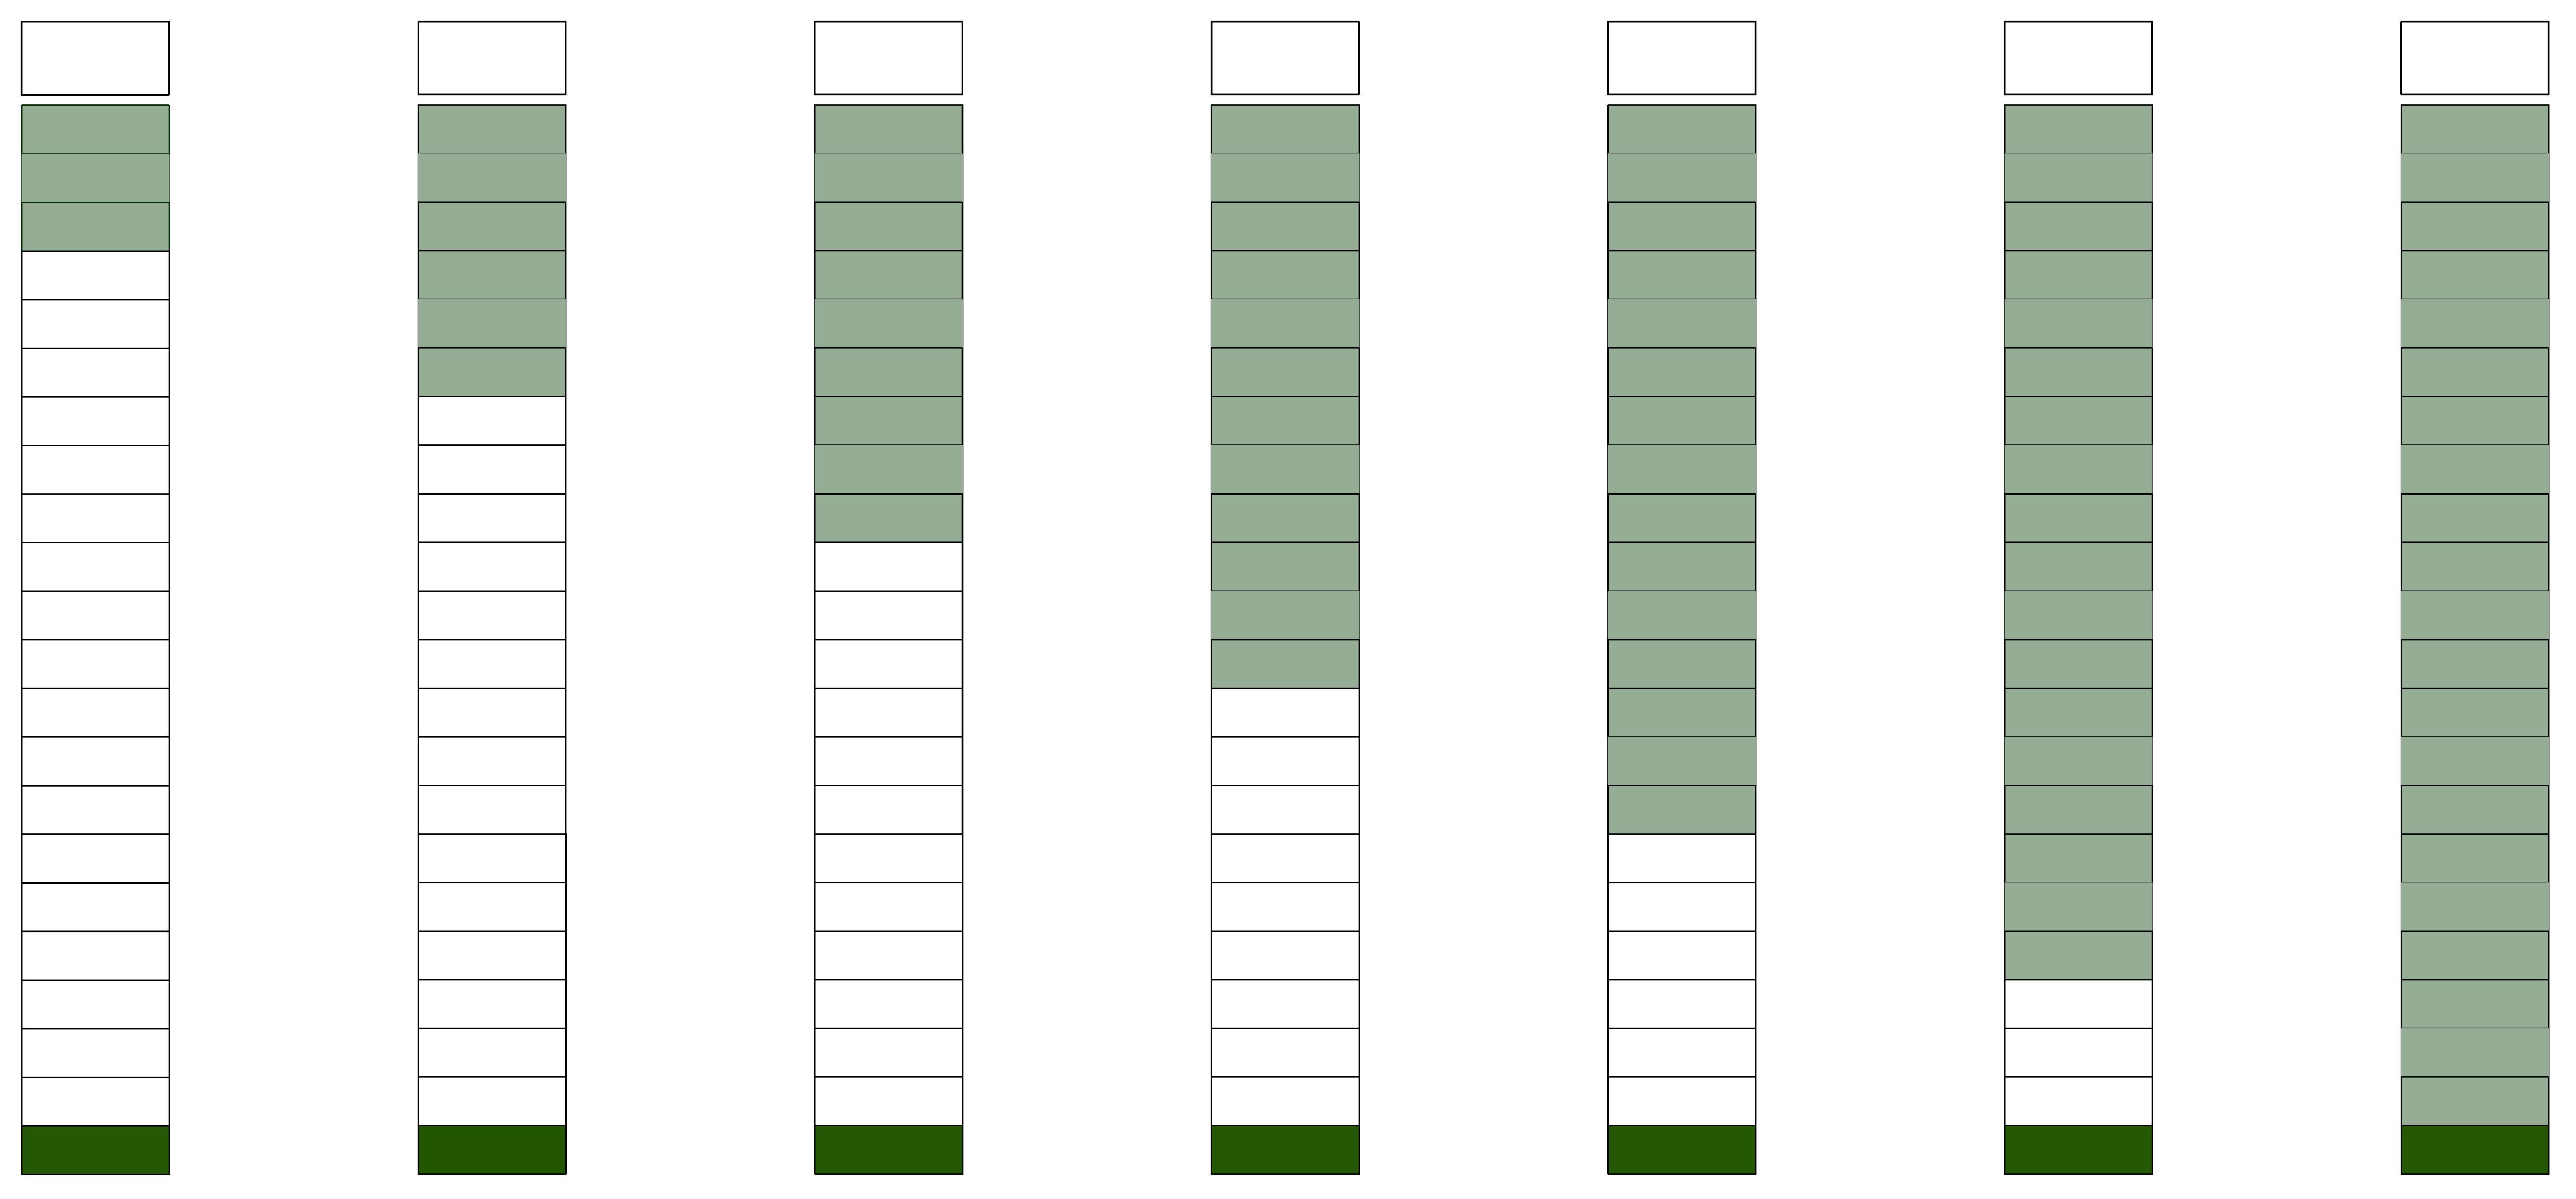
\includegraphics[width=0.9\columnwidth]{masse.pdf}
		\caption{\footnotesize{\textbf{Mass distribution in a vorespace.} The vorespace can be seen, according to the mass, as composed of 3 parts: 1 of 20 states corresponding to the equilibrium state (first white box), followed by 21 boxes representing each gravity-charge pair and finally the blocking state, in dark green. Fractality requires that the distribution be made in 7 jumps, therefore by a jump of 3 double pairs (in light green)}}
	\end{figure}
	
	Note that this model of mass distribution is very Hamiltonian. 
	If $\omega$ is the energy of the system, which is the case, then the 128 
	possible states of the mass represent the phase space of its distribution. 
	It is a Hilbert space of dimension 7 ($2^7=128$) and the $\omega$ are the 
	eigenstates of the system.
	
	However, having so many masses poses a problem of simplicity 
	in our model of quantum plenodynamics. Still due to the 
	principle of Occam's razor, we will stipulate that there is only one type of mass 
	to build the standard model of physics and we will choose the 
	heaviest, $\omega_m$. We will justify this hypothesis in the Big Bang 
	cosmological model.
	
	We will develop the consequences of such a mass model in the 
	part on gravity.
	
	\subsection{Electric charge}
	
	Just as mass is a topological aberration of the plenum, and therefore of its
	physics, electric charge is part of its nature. It is therefore logical 
	to manage this charge with the physics of the plenum alone.
	
	We define the electric charge $q_v$ of the vorespace as the stable state 
	of the turbine, i.e., the state of positions 1 to 20. In a way, the electric 
	charge is its maximum flux (or its nominal flux). As the flux decreases 
	until state 64, the charge also decreases. It cancels out at the 
	"center", then reverses. The sign changes and the charge grows 
	negatively (or positively, if we start from a negative charge). 
	It will reach its full charge $-q_v$ in states 108 to 128.
	
	Unlike the case of mass, the case of electric charge is therefore 
	not blocked at the moment of the cancellation of the charge. The 
	physics of the plenum in no way forbids the charge from exploiting 
	all the capacities of the vorespace.
	\vspace*{-0.5cm}
	\begin{center}
		\begin{longtblr}[
			%theme=widecaption 
			caption={\footnotesize{\textbf{Vorespace charge}}},
			%label = {tblr:4-2},
			]{
				colspec={Q[c,m] Q[1.5cm,c,m] Q[, c,m] Q[2cm,c,m] Q[1.9cm,c,m]},
				rowspec={Q[m]},
				row{odd}={bg=blue!10!white},
				row{1}={c,mode=text,fg=white,bg=pkcolor, cmd=\textbf}, %cmd=\textbf, blue!80!orange
				rowsep=2pt, colsep=3pt,
				vline{2-Y} = {1}{0.3pt,gray!50},
				vline{2-Y} = {2-Z}{0.3pt,gray!30},
				hline{Z} = {0.1pt,blue},
				% nombre de col début et fin qui apparaissent à chaque page
				% 1 pour le titre par exempel
				rowhead = 1, %rowfoot = 1, 
			}
			States   & Number of states &  Charge  &  Charge evolution &  Direction of rotation     \\
			1-19    &   20       &  $+q_v$  &        stationary      &       chiral           \\
			20-61   &   42       &  $+q_v$  &        decreasing            &       chiral           \\
			62-65   &    4       &    0     &      stationary        &        none           \\
			66-107  &   42       &  $-q_v$  &        increasing          &      anti-chiral      \\
			108-127 &   20       &  $-q_v$  &        stationary      &      anti-chiral      \\
			
		\end{longtblr}
	\end{center}
	
	As all the physics of the plenum is managed by a 7-step fractal law, the 
	electric charge is no exception to the rule. The stable nodes being the 
	stationary charges, the progression must be divided over the 90 intermediate 
	states. On the other hand, for the same reasons as mentioned in the case 
	of mass, these states go in pairs. But this time, the physics of the 
	charge concerns only the tilt of the blade. As tilting the blade also 
	leads to adapting its shape, and therefore the charge variation, the 
	variation in tilt goes hand in hand with the modification of the shape of 
	the blades. The double pair 62-65 being stationary, and thus a stable 
	state, it does not count in the transition states. We therefore have 84 
	transition states, i.e., 42 possible pairs. With a fractality of 7, 
	\textit{the charge varies by groups of 6 pairs.}
	
	There are two immediate consequences. The first is that the charge varies 
	by thirds. It passes from $q_v$, to \Ru{+}{2}{3}{e} and to \Ru{+}{1}{3}{e} before 
	canceling out, then resuming an inverse progression. Finally, the 
	progression of the "electric variety" is twice as fast as that of the 
	mass. Here is a beginning of an explanation for the domination of the 
	electric force over the force of gravity.
	
	We will now be able to study these forces in more detail.
	
	
	\subsection{Electric and gravity forces}
	
	\subsubsection{Introduction}
	
	The plenum model fabricated previously suffers from a serious flaw. It is 
	static. How to build the elementary particles of the standard model 
	without dynamics? It is impossible! We must therefore find a way to 
	create this dynamics. We will establish that it comes (in part) from 
	electric and gravity forces. To this end, we will look into these 
	forces, even if, as we will see, it will be necessary to postulate the 
	existence of a charged particle to complete the demonstration of electric 
	forces. The dynamics, responsible for the birth of the elementary 
	particles of the standard model, will thus initiate thanks to gravity, 
	then consolidate through the cumulative effect of electrodynamics. It 
	is a very cosmological model, but quantum plenodynamics does not 
	pretend to reinvent physics! We will see however in the Big Bang 
	cosmological model that masses also possess an initial energy dispersion 
	velocity, because of the expansion of the initial "black hole".
	
	Although we could here focus only on gravity as a triggering element, the 
	fact that electric and gravity forces are linked gives meaning to 
	addressing them together. We will highlight the existence of magnetic 
	monopoles and their role in gravity, connecting the visions of Paul 
	Dirac and Georges Lochak. We will also establish that the vector 
	potential of electromagnetism is a real physical field and, above all, 
	that there are two of them: gravity phonons and charge phonons. From there, 
	quantum plenodynamics will make its first prediction: charge slows 
	down time, as mass does too. We will finally deduce an explanation for 
	the Aharonov-Bohm and Aharonov-Casher effects, which will be the first 
	two experimental proofs of the veracity of the quantum plenodynamics 
	model.
	
	\subsubsection{The electric force}
	
	The basic mechanism of the electric force is quite simple. The vorespace 
	is chiral and possesses a screw thread. The interaction between two 
	neighboring vorespaces occurs structurally via this screw thread. The 
	simplistic vision is that of a gear: if one turns in one direction 
	(chiral), the next one necessarily turns in the other (anti-chiral).
	
	This is the basis. Two vorespaces of opposite chirality are structurally 
	linked (this is the attractive force of particles of the same sign), 
	while two vorespaces of the same chirality cannot meet without blocking 
	their rotation and breaking the plenum. \textit{The electric force is 
		therefore consubstantial with the plenum}. It ensures not only its 
	electrical neutrality but also its shape. If the plenum is static from a 
	structural point of view, it is dynamic from an energy point of view. It 
	can be seen as a permanent exchange of flux from one vorespace to 
	another. By analogy with fluid mechanics, the vorespace acts as a 
	turbine for the information fluid. The movement of the fluid is a pure 
	vortex, a whirlwind. To circulate, the fluid relies on the blade which, 
	in return, balances itself by gyroscopic effect. This effect has all the 
	characteristics of the magnetic field. It is perpendicular to the blade, 
	in the opposite direction of the fluid's pressure. It respects the 
	three-finger rule relative to the fluid's movement. Since it exists in 
	each vorespace without looping, it is a monopole.
	
	The magnetic monopole is therefore not \textit{stricto sensu} a 
	particle\footnote{We will modulate this statement later by showing that a particle having the property of a magnetic monopole actually exists}, 
	but the restoring torque of a vorespace in reaction to the passage of 
	the flux. The existence of the monopole was predicted by Paul Dirac in 
	1931 \cite{dirac1931quantised}. In the case of the plenum's vorespace, given the 
	alternation of vorespaces, the magnetic monopoles cancel each other out in 
	pairs. Consequently, the magnetism of the plenum is zero. On the other 
	hand, as soon as we leave the nominal case of the plenum, by adding mass 
	or by touching the 88 potential positions, it is possible to make a 
	non-zero monopole appear.
	
	Nothing else can be extracted from the static model of the plenum. To 
	move forward, let us postulate the existence of a charged particle in the 
	plenum by anticipating its elaboration in the following chapter. In any 
	case, its existence is plausible, because it exists in the elementary 
	particles of the standard model of physics. The chirality of the 
	particle is not neutral with respect to the plenum. If one concentrates 
	in a compact place a super-chirality, a break in the continuity of the 
	plenum occurs around the particle. This is structurally impossible: the 
	plenum is a rigid crystal. If a rupture occurs, a vacuum is created, a 
	real vacuum, an absence of vorespace. The plenum must therefore adapt.
	
	The charge is directly related to the angle of rotation of the screw (in 
	reality, its two possible tilts). At the boundary between the massive 
	particle and the plenum, the vorespaces have no other choice but to 
	"twist" in order to make the gear slip. Twisting means adapting the gear 
	angle. All the peripheral vorespaces to the particle are concerned. Of 
	course, it is impossible to absorb on a single row the balance rupture 
	caused by the charged particle. Step by step, each row of vorespaces 
	twists in order to spread the catch-up angle until the nominal angle of 
	the vorespace. Visually, at the level of the turbine blades, a 
	\textit{shear} is created starting from the charged particle.
	
	This phenomenon describes a standing wave. The charged particle acts as 
	a standing wave on the plenum in order to ensure the continuity of the 
	plenum so as not to break it. The shape of the wave depends of course on 
	the shape of the particle, but above all on the way it is transmitted. 
	The medium being fractal, it can only be transmitted in steps, according 
	to a rhythm of 7 steps before looping back. The wave is thus an open 
	heptagonal rosette, in the manner of what can be observed in photos of 
	novas when they suck in galaxies. The analogy is not necessarily 
	fortuitous: if the universe follows a fractal law, it is normal to find 
	the same images at all scales$\dots$
	
	We have therefore created a structural gradient concerning the angle of the 
	double helices. Technically, the wave also varies at the heart of the 
	vorespace, because of the double helicity, but from a macroscopic point of 
	view, the statement of the gradient remains correct. It is a shear wave. 
	In solid state physics, this wave is called a phonon. As the plenum is a 
	crystal, by analogy, we will call this compensation wave of static 
	tension of the electric charge a \textit{charge phonon}.
	
	An immediate consequence is that the disturbance of the angle (open or 
	closed), without changing the rotation value of the vorespace, induces a 
	drop in the efficiency of the vorespace. Indeed, the vorespace must 
	"draw" from one of the 108 potential positions to adapt. It is no longer 
	in its nominal shape. The duration of exergy transfer must therefore 
	increase.
	
	\textbf{Time therefore slows down near an electric charge!}
	
	It is clear that this phenomenon will not be easy to observe at our 
	scale, because the accumulation of necessary charges risks being 
	disturbed by a breakdown effect$\dots$
	
	\subsubsection*{How to explain the electric force?}
	
	It is a purely exergetic effect, because the electric force concerns 
	chirality, which is intrinsic to the plenum. The force will therefore be 
	managed by the physics of the plenum, which is thermodynamics.
	
	Each charged particle creates a charge phonon which is a heptagonal 
	standing wave. When two particles approach, the waves interfere. When 
	two particles have the same charge, the waves add up and the vorespaces 
	increase their structural energy (sum of the energies of each phonon). 
	The crossing time increases, because the crossing is increasingly 
	costly. The particles will favor the lowest energy paths (the thalweg), 
	which are opposite. They will move back from each other. \textit{A 
		contrario}, particles of different charges attract each other by 
	minimizing the energy on the meeting path.
	
	\subsubsection*{What is the electric field?}
	
	\textit{The electric field is the gradient of the phonon}. It is therefore 
	the slope of the shear wave (which is continuously ascending or 
	descending at the macroscopic scale, passing through an adaptation 
	within the two helices of each vorespace).
	
	As the plenum is a crystal, we can apply Hooke's law which stipulates 
	that, for a crystal in shear, the exergetic cost of the transfer is 
	proportional to the square of the cell's deformation. In classical 
	mechanics, one finds that the energy of the field is proportional to 
	$E^2$. In the plenum, the correspondence is that the consumed exergy is 
	proportional to the square of the amplitude of the stationary torsion 
	wave.
	
	\subsubsection*{What is the magnetic field?}
	
	The magnetic monopole alone does not allow for the induction of what the 
	magnetic field is. The only solution is to find a shape that allows the 
	looping of the field on itself, as is expected. Its construction is 
	outside the scope of this part. By anticipation, we can say that a 
	candidate exists: it is the hopfion.
	
	\begingroup
	\enlargethispage{0.38cm}
	\endgroup
	\begin{figure}[H]
		%\captionsetup{width=5cm}
		\centering
		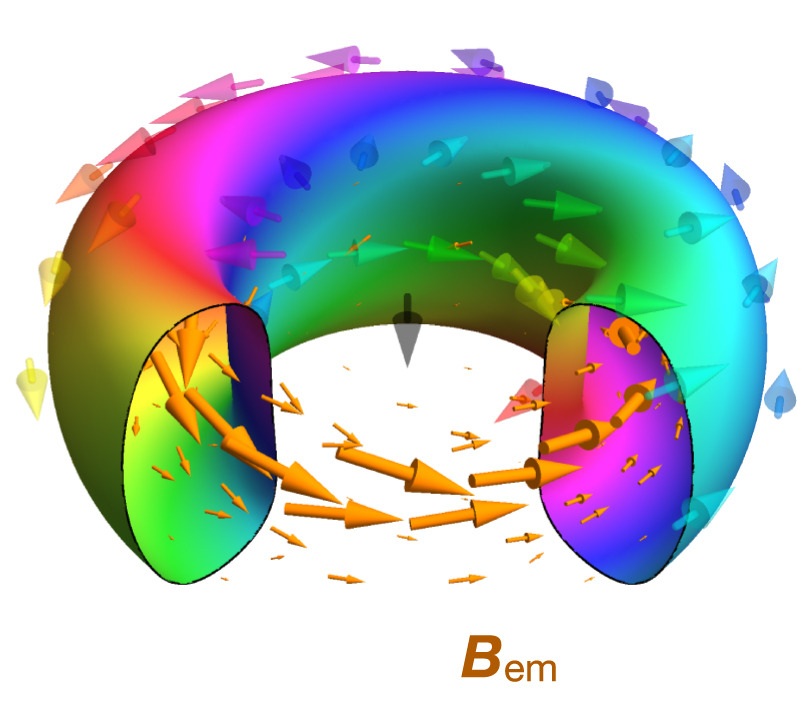
\includegraphics[width=0.9\columnwidth]{Hopfion.png}
		\caption{\footnotesize{\textbf{The hopfion.} It is the first stable node of the plenum that acts as a magnetic dipole. We will see later that it resembles an $S_1$ or $S_4$ node. (credit: Wikipedia)}}
		\label{figure:1-hopfion}
	\end{figure}
	
	
	We note that the field $\vec B$ being always perpendicular to the blade 
	and that the charge phonon creating a "blade slope continuity" in the 
	plenum, the resulting field $\vec B$ is indeed perpendicular to this 
	"blade wave", in accordance with what the laws of electromagnetism 
	describe.
	
	\subsubsection{The force of gravity}
	
	Unlike the electric force which requires, to study it, postulating the 
	existence of a charged particle, it is possible to create a mass 
	vorespace (which is by no means obvious to prove \textit{in se}. We can 
	postulate it virtually for this part, but its existence will have to be 
	proven later. Fortunately, the Big Bang model allows for the creation of 
	these particles$\dots$) However, this is not without consequence. We 
	have seen that mass deforms the turbine and forms a topological plug. 
	The plenum must ensure continuity around the mass, so as not to tear 
	itself apart.
	
	Just as the angle varies for the electric charge, it is now the shape of 
	the blade that will adapt to ensure this continuity. Although the 
	result is substantially identical in shape to that of the charge phonon, 
	the prevailing dynamics is radically different. It is the constraint of 
	the blades that gives an identical result, but the dynamics rests on the 
	shape in the tilt-shape pair. Similarly, for the electric charge, the 
	dynamics bears on the tilt. Like what happens for the electric charge, a 
	\textit{mass phonon} will be created to ensure the continuity of the 
	plenum in the presence of a mass.
	
	One could have postulated that the mass yields speed to the surrounding 
	vorespaces to ensure this balance. This would have meant that the mass 
	creates mass around it, by yielding some of its own mass. The 
	phenomenon having never been observed, it was not retained. The mass 
	therefore creates a mass phonon, that is to say a mass wave. It is also a 
	standing wave, heptagonal. The gradient is the expression of the 
	gravitational field.
	
	Warning: the gradient acts at the same time on the crest of the 7 waves, 
	but also between the 7 wave crests, via a double gradient$\dots$ Mass 
	wave thalwegs are thus created.
	
	We have furthermore seen that the physics of mass on the plenum is no 
	longer thermodynamics, but flux physics. Note then the deep link that 
	appears with the magnetic monopole. Indeed, the magnetic monopole is the 
	gyroscopic effect, the counter-reaction of the blade to the passage of 
	the flux. If this effect is zero in the plenum, the mass phonon 
	transforms the shape of the blade to precisely create a brake on the 
	flux. Gravity and the magnetic monopole are therefore intrinsically 
	linked. This idea joins that of Georges Lochak on the necessity of 
	having a mass for the magnetic monopole \cite{lochak2002monopole}. We will see 
	moreover in the standard model that it is possible to create a particle 
	meeting the criteria of a magnetic monopole and that this particle will 
	be a neutrino, as Georges Lochak suspected \cite{lochak2002monopole}.
	
	Of course, as the flux around the mass is disturbed by the mass phonon, 
	the information flow is no longer optimal, i.e., analogous to that of 
	the plenum's vorespace. The crossing time increases.
	\medskip
	
	\textbf{In the presence of a mass, time slows down.}
	
	\subsubsection*{What is the force of gravity?}
	
	Let us analyze what happens when two masses are close to each other. We 
	are now in a flux physics. There are two scenarios, but they have 
	analogous results regarding their effects. Nothing at this stage of 
	reflection forbids the existence of a chiral or antichiral mass. 
	Technically, this amounts to having a mass that screws into the plenum 
	(on a plane, we would form a bell, like a ball on a sheet) or that 
	unscrews (still in a plane, the image would be a ball pushing under the 
	sheet, vertically).
	
	Opposite the two masses, their respective mass phonons interfere. The 
	flux, already reduced, decreases further. A flux imbalance is created 
	between the masses and around the masses. In hydraulics, a flux 
	gradient draws the object toward the calmest flux. This is the thalweg 
	of the flux. Each mass therefore moves toward the other, "rolling in the 
	thalweg". \textit{This is the force of gravity.}
	
	It should be noted here that gravity respects thermodynamics. If the flux 
	decreases, exergy drops. From a purely energy point of view, the two 
	masses move toward an energy minimum, an energy thalweg. To lower 
	exergy without changing the rotation speed of the vorespace, it is 
	necessary to draw from the reserves of the 88 possible positions. This is 
	an increase in entropy. The thalweg is literally a depression of 
	negentropy, the line of steepest slope toward the most "probable" 
	state. Louis de Broglie had illustrated it with this thalweg image: "the 
	natural trajectory follows the thalweg of a negentropy valley." 
	\cite{debroglie1964thermodynamique}
	
	Here we must properly understand what happens when two chiral and 
	anti-chiral masses meet. The masses are then in phase opposition. One 
	pulls up, the other down. Their meeting is a return to balance. 
	Technically, there is a symmetry breaking. The entropy extracted from 
	the plenum is returned to it and it is again stored potentially. The 
	plenum is back at equilibrium (provided of course that the chiral and 
	anti-chiral masses have the same mass, otherwise the difference forms a 
	new mass, of entropy of the difference of entropy of the two previous 
	masses). We will see later that, in any case, this case is not very 
	interesting, because it is just an aberration created in our particle 
	accelerators. The case of two masses of the same chirality is much more 
	interesting. From a hydrodynamic point of view, there is no reason why 
	two masses should not meet. Of course, they cannot be superimposed, 
	because it is not possible to overlap two vorespaces: the rigidity of the 
	plenum forbids it. On the other hand, the fusion dynamics of the 
	fractal law that governs the plenum authorizes (and encourages) the 
	fusion of two masses. Two masses do not overlap: they merge into a 
	single mass, respecting in passing the spatial scale of the fractality.
	
	Gravity is therefore the engine of the fusion of our fractal model. Of 
	course, we sense that, if the meeting between two masses is 
	indispensable, the plenum, because of the intensity of the fluxes at 
	the moment of the meeting, will undergo a considerable tension, a 
	tension that will have to be transformed into something. This something 
	will be the photon and we will study it as the first particle of the 
	standard model, even if \textit{stricto sensu} it is rather a waste 
	product of the process.
	
	\subsubsection{Some consequences}
	
	\paragraph{The vector potential}~\\ 
	
	The mass and charge phonons, if they are extremely similar in their 
	appearance, are radically different in their creative principle. The 
	charge phonon is a shear wave and the mass phonon is a flux wave. From 
	their respective gradients, we can extract a known physical quantity, 
	the gravitational constant and the electric field.
	
	As always in quantum plenodynamics, these fields are therefore real 
	physical fields. We can obviously link the charge phonon to the vector 
	potential of magnetism, resulting from the rotational of the magnetic 
	field. Magnetism postulates a field of purely mathematical vectors. 
	This field is certainly the charge phonon. It thus indeed exists. As we 
	have seen that magnetism and gravity are intimately linked, the mass 
	field is also a materialized vector potential. These are the two facets 
	of the same field, used differently. This is why quantum 
	plenodynamics differentiates them.
	
	Similarly, David Bohm's quantum potential \cite{bohm1952suggested}, in his theory of 
	de Broglie's pilot-wave, is directly the phonon that guides the 
	particle. We will develop this point when we establish the compatibility 
	between quantum plenodynamics and quantum mechanics.
	
	\paragraph{The Casimir effect}~\\
	
	A direct and intuitive application of phonons is the Casimir effect. By 
	putting two plates opposite each other which are bombarded with energy 
	on their opposite face, a force is created that sucks the plates 
	against each other.
	
	By bombarding each face, the energy value at the level of the plates is 
	increased. To ensure a continuity of the plenum, a mass phonon is 
	created. The interface of the phonons between the plates creates a drop 
	in flux which creates a depression, and thus the attraction of the two 
	plates.
	
	\begin{mybox}[breakable,colback=blue!10, colbacktitle=pkcolor]{The force of gravity}
		The attractive force is therefore a generalized Casimir effect between two 
		masses.
	\end{mybox}
	\medskip
	
	
	\paragraph{The Aharonov-Bohm and Aharonov-Casher effects}~\\
	
	
	If quantum mechanics still manages to explain the Casimir effect by 
	mobilizing "vacuum energy", which is a way of seeing the mobilization of 
	the entropic reserve of the plenum that is the phonon, it does not 
	explain the Aharonov-Bohm and Aharonov-Casher effects.
	
	When an electron is passed between two slits, an interference pattern 
	classically forms on a projection plane, if the dimensions of the slits 
	are of the order of the electron's wavelength. On the other hand, 
	placing a charged solenoid near the path of the electron disturbs the 
	interference pattern, causing a phase delay to appear.
	
	The magnetic field $\vec B$ being present --~according to the laws of 
	electromagnetism~-- only inside the solenoid, how does an electron 
	"feel" the presence of the field, while it passes outside the solenoid? 
	Current physics does not explain it.
	
	In reality, the boundary at the level of the solenoid cannot be brutal at 
	the level of the plenum. A charge phonon is created outside. The 
	electron crosses this phonon, which is no longer a balanced plenum. 
	The crossing time increases. The phase shifts.
	
	An experimental proof of the existence of this phonon would be to move the 
	solenoid back. There exists a distance at which the charge phonon 
	balances with the plenum. The electron would then no longer be 
	out of phase. An experiment with a series of increasing distances 
	should highlight a decreasing phase delay.
	
	Similarly, classical physics does not explain the Aharonov-Casher effect. 
	This time it involves circulating a particle having a magnetic moment, 
	like a neutron for example, along a charged line. This time a shift in 
	the spin angle is created. In the absence of a magnetic field, this 
	phenomenon is inexplicable. The presence of a charge phonon, due to the 
	electric line, explains the presence of the perturbing field. 
	Similarly, we should be able to highlight the field cut-off distance 
	via a protocol similar to the previous one.
	
	\subsubsection{Conclusions}
	
	The electric force, consubstantial with the plenum, is governed by 
	thermodynamics. The force of gravity, unnatural to the plenum, is 
	governed by a physics different from the equilibrium physics of the 
	plenum. It is a flux physics. These two forces reveal, each in its own 
	way, a torsion of the plenum to ensure its continuity without 
	breaking it. As the plenum is a crystal, these are two phonons, of 
	charge and mass. In reality, the two phonons are linked: torsion is the 
	engine of one and flux management the engine of the other. They are 
	the two sides of the same coin, according to how they are used. The 
	gradient of the phonons then gives the values of the electric and 
	gravitational fields. We note that the gravitational field and the 
	magnetic field are linked by the same mechanism. Finally, the 
	magnetic monopole exists as a gyroscopic effect of the blades of the 
	vorespace at the passage of the entropic flux. It cancels out at 
	equilibrium and reveals itself of course when entropy increases.
	
	
	\section{The standard model of physics}
	
	\subsection{Introduction}
	
	For the moment, the proposed model is satisfactory, because it is 
	compatible with electromagnetism and gravity. It further explains the 
	Aharonov-Bohm and Aharonov-Casher effects, which is no small feat. It 
	must now explain the creation of the elementary particles of the 
	standard model to be validated.
	
	It is first necessary to uncover the true nature of the photon. Indeed, 
	until now, physics only noted the existence of the photon and took note 
	of it. We are going to answer the big question that Albert Einstein 
	asked himself: "If only we could understand $E=h\nu$!"\cite{einstein1994correspondence} 
	We will discover that the photon is outside the model, because it is, 
	like the force of gravity, an anomaly of the plenum. But instead of 
	being an anomaly using vacuum potential, it is an anomaly of 
	structure, of dimension.
	
	\subsection{The photon}
	
	\subsubsection{The model of the photon}
	
	The problem consists in building a photon from the vorespaces of the plenum, 
	whether they are mass-bearing or not. These are indeed the only "tools" at our 
	disposal and we cannot do otherwise than use them.
	
	The difficulty is to create a spin-1 particle from spin-\R{1}{2} particles. 
	The obvious solution is to assemble two spin-\R{1}{2} particles. In the 
	plenum, two consecutive vorespaces are alternated, to ensure electrical 
	neutrality, but also zero spin. It is therefore necessary to flip a 
	vorespace to put two of them face-to-face. The screw head of one thus faces 
	the screw point of the other. The sum of the spins is indeed 1: the 
	"double-vorespace" is a boson. Louis de Broglie's image of a photon 
	composed of two half-photons takes shape. \cite{debroglie1934une}
	
	Two problems arise instantly. It is impossible to flip a vorespace in the 
	plenum without tearing the plenum itself, as it is rigid. Technically, it 
	is therefore impossible to create a photon by the fractal law of the 
	plenum.
	
	Suppose, however, that this were possible. This double-vorespace is in 
	reality a pair (vorespace, anti-vorespace). The two vorespaces are 
	identical in every way, but in a mirror fashion. They must annihilate 
	each other. What is this process, where does it come from, and what 
	does it ultimately produce?
	
	The creation of a photon in the plenum is \textit{a priori} a structural 
	impossibility. The photon is technically a topological aberration, and its 
	development process is contrary to the laws of the plenum. Fortunately, 
	gravity comes to the rescue of the photon.
	
	Let us return to the moment when two masses approach to merge. Their mass 
	phonons add up, creating hyper-entropic vorespaces along the path. Their 
	speed is still $\omega_v$, but the shear wave literally crushes the 
	turbine by flattening it: a moment comes when the turbine becomes a 
	"disk", obstructing all passage. The flux is then cut off. The approach 
	of the masses being symmetrical, it is certain that at least two 
	neighboring vorespaces have reached this state.
	
	The pressure on the vorespaces becomes gigantic, since on one side the 
	flux is zero and, on the other, it is very large. Everything is blocked. 
	However, the mass has a velocity that exceeds the rotation speed of the 
	blocked plenum. It can therefore still force through by yielding part of its 
	excess energy. The additional screw turn thus overcomes the resistance of 
	the plenum, which "cracks". To make the plenum crack, the mass must 
	therefore yield an energy corresponding to the mass of the vorespace, i.e., 
	$\omega_v$.
	
	Visually, the two vorespaces, which are disks, enter into one another. The 
	penetration occurs at the expense of the surface area. In 7 steps, it is 
	completely torn away. At the 8th step, the two spheres become two 
	intertwined disks.
	
	Concretely, the vorespaces have lost their surface area, which came from 
	the 3rd degree of freedom. The two circles are thus a vorespace with two 
	degrees of freedom. We could then amuse ourselves by developing many 
	theories to find out what this new assembly looks like, but that has 
	already been done. It is still a Clifford bivector, but with two degrees of 
	dimension, a v-sphere $S_2$. It is composed of two perpendicular circles 
	that have a linked rotation, allowed around an axis that connects them by 
	"welding" them around two fixed points.
	
	The best image one can have of it is that of a universal joint (cardan).
	
	One notices immediately that two circles in linked rotation form a photon. 
	Gravity, by bending the plenum, has thus created a photon.
	
	The process is not finished. The masses continue their push on the photon 
	which begins to rotate. It obviously turns according to a 7-step 
	process, thus in steps of $2\pi/7$. At each step, the two circles wrap 
	around a neighboring vorespace and, at the seventh, they are completely 
	wrapped. One then notices that the photon itself has only made a half-turn. 
	Nothing slows down the photon, as it does not interact with the 
	vorespace. It can therefore only continue to wrap itself. At the end of the 
	second vorespace, it finishes its own full rotation. It thus takes two 
	vorespaces to perform a full rotation, confirming de Broglie's intuition 
	that the photon is composed of two half-photons. In reality, its lower 
	dimensionality forces it to adapt to its new space.
	
	Nothing stops the photon anymore, which always wraps according to the DNA 
	strands of the plenum. It therefore circulates at the nominal transmission 
	speed of a vorespace, that is to say at c.
	
	\subsubsection{The consequences}
	
	There is a wealth of information in the previous process. The photon is a 
	symmetry breaking of the plenum, which is a thermodynamic equilibrium. As 
	a topological anomaly, its co-existence in the plenum as a static 
	particle is impossible: the photon is not part of the plenum's universe. 
	Its dynamics is therefore a response to this impossibility: it is 
	condemned to flee, being unable to stay still. Without mass, it 
	circulates like a superfluid, at the maximum speed allowed by the plenum. 
	But its speed and its mass are also a means of conserving the static mass 
	of the plenum, without which the disappearance of two vorespaces would 
	change the global equilibrium of the plenum. The total energy is indeed 
	conserved. Each merged mass has lost the energy of one vorespace, thus 
	decreasing its rotation by $\omega_v$.\footnote{We will see in reality that 
		the process is dynamic and that the exergetic cost is deducted from the 
		movement.} The total energy of the plenum has not been modified.
	
	One consequence is that the physics of the photon is also different from 
	that of the plenum, which is purely exergetic, like that of the electric 
	force. Gravity, for its part, is a flux physics. The physics of the photon 
	thus rests solely on entropy. The photon is in a way an \textit{entropic 
		revealer}. Through its double-mechanism of interlocking, of the opening of 
	the photon and the rotation of the screw of the vorespace, the passage of 
	the photon is literally "stuck" to the vorespace and follows it in all its 
	entropic fluctuations. 
	
	Consequently, the photon not only decodes the entropy of the vorespace, but 
	always moves toward the positive gradients of the phonon, that is to say by 
	"surfing on the entropic crest" or, as Louis de Broglie put it, "by 
	following the thalwegs of negentropy". In other words, it is the second law 
	of thermodynamics that is brought to light, not as a principle born from 
	human experience, but as a mechanical constraint between a photon and a 
	vorespace. 
	
	\begin{mybox}[breakable,colback=blue!10, colbacktitle=pkcolor]{Second law of thermodynamics}
		The second law of thermodynamics is in reality a structural mechanism.
	\end{mybox}
	\medskip
	
	Furthermore, the creation of the photon allows the completion of the 
	development of fractal mass fusion. It is necessary that there be an even 
	number of vorespaces between the masses. When the group of pairs or the 
	pair of vorespaces reaches its maximum entropy, then gravity can 
	transform them into photons, to finish opening the way. When there are no 
	more vorespaces between them, the masses are in contact. \textit{This is 
		fusion}. It is likely that photon emission also follows a law of 
	creation by groups of 7.
	
	Finally, the photon, as a sub-product of gravity, reveals in a mirror 
	fashion an underlying structure of the plenum. If one can break the 
	symmetry of particles, one can break the symmetry of the entire 
	structure. \textit{One then senses that the plenum is the result of a 
		previous two-dimensional structure via a fractal passage}. The photon is 
	thus a resurgence of the past. We will see later, thanks to the Big Bang 
	model, that it is in reality like a young driver who discovers the 
	intoxication of speed. In any case, this "justifies" the assumed energy 
	distribution, dividing by two in the "rear fusion". The fractal law must 
	be respected in the change of scale. We will return to all this when we 
	address the Big Bang model.
	
	\subsection{The model of elementary particles of the standard model}
	
	Let us now tackle the construction of the elementary particles of the 
	standard model of physics. To this end, we will postulate an abundance of 
	elementary masses of velocity $\omega_m$. The fusion process will occur 
	via gravity and will follow a fractal process that is not 
	dimensionally restricted.
	
	As a reminder, the list of elementary particles to be created is shown in 
	Table \ref{tblr:4-epe}.
	
	\clearpage
	\begin{center}
		\begin{longtblr}[
			%theme=widecaption 
			caption={\footnotesize{\textbf{Energy of elementary particles}}},
			label = {tblr:4-epe},
			]{
				colspec={Q[c, co=1]  Q[c] Q[c, co=1] },
				rowspec={Q[m]},
				row{odd}={bg=blue!10!white},
				row{1}={c,mode=text,fg=white,bg=pkcolor, cmd=\textbf}, %cmd=\textbf, blue!80!orange
				rowsep=2pt, colsep=3pt,
				vline{2-Y} = {1}{0.3pt,gray!50},
				vline{2-Y} = {2-Z}{0.3pt,gray!30},
				hline{Z} = {0.1pt,blue},
				% nombre de col début et fin qui apparaissent à chaque page
				% 1 pour le titre par exempel
				rowhead = 1, %rowfoot = 1, 
			}
			Particles               &   Designation         & Mass                     \\
			Photon                   &        $\gamma$       &  0                       \\
			Gluon                    &            g          &  0                       \\
			Electron neutrino        &        $\nu_e$        &  < 0.8 $eV/c^2$           \\
			Muon neutrino            &        $\nu_\mu$      &  < 0.17 $MeV/c^2$         \\
			Electron                 &            $e^-$       &  0.511  $MeV/c^2$         \\
			Quark up (u)             &            u          &  $\approx$ 2.2 $MeV/c^2$ \\
			Quark down (d)           &            d          &  $\approx$ 4.7 $MeV/c^2$ \\
			Tau neutrino             &        $\nu_\tau$      &  < 18.2 $MeV/c^2$         \\
			Muon                     &        $\mu^-$        &  105.7 $MeV/c^2$          \\
			Quark strange (s)        &            s          &  $\approx$ 95 $MeV/c^2$  \\
			Quark charm (c)          &            c          &  $\approx$ 1.28 $GeV/c^2$\\
			Tau                      &          $\tau$        &  1.77 $GeV/c^2$           \\
			Quark bottom (b)         &            b          &  $\approx$ 4.18 $GeV/c^2$\\
			W boson                  &          $W^\mp$       &  80.4 $GeV/c^2$           \\
			Z boson                  &            $Z_0$       &  91.2 $GeV/c^2$           \\
			Higgs boson              &            $H_0$       &  125.1 $GeV/c^2$          \\
			Quark top (t)            &            t          & $\approx$ 173 $GeV/c^2$ \\
		\end{longtblr}
	\end{center}
	
	
	It will therefore be necessary to fit this list into a fractal process. Now, the 
	fractal process of Clifford algebra was initially chosen, namely 7 possible 
	nodes, $S_1$ to $S_6$. These nodes will therefore be composed of mass-bearing 
	vorespaces, in progression of the fractal law.
	
	We can represent them and obtain some characteristic information (\textit{cf.} 
	Table \ref{tblr:5-0-1}). A natural composition from $S_1$ to $S_6$ clearly 
	appears, with three forms (circle, double-circle, and helix), with a break 
	in composition for the 7th form which is an end in Clifford algebra.
	
	Let us therefore postulate that at this scale, the end of the process 
	leads to our first physical particles, the hadrons, namely the neutron and 
	the proton. Technically, the neutron and the proton would be $S_8$ nodes.
	\vfill\strut
	
	%\vspace*{-0.5cm}
	\begin{table}[H]
		\centering
		\caption{\footnotesize{\textbf{Nodes of the Clifford algebra $S_{7,0}(\mathbb{R}$)}}}
		\label{tblr:5-0-1}
		\begin{tblr}[
			%theme=widecaption 
			%        caption={\footnotesize{\textbf{Nodes of the Clifford algebra $S_{7,0}(\mathbb{R})$}}},
			%        label = {tblr:5-0-1},
			note{$\dagger$} = {composed of vorespaces, thus it is a sequence resembling the DNA strand, a continuous tube varying from a maximum to a minimum.},
			]{
				colspec={Q[c,m]  Q[2cm, c,m] Q[4cm,c,m] Q[c,m] },
				rowspec={Q[c,m]},
				row{odd}={bg=blue!10!white},
				row{1}={c,mode=text,fg=white,bg=pkcolor, cmd=\textbf}, %cmd=\textbf, blue!80!orange
				rowsep=2pt, colsep=3pt,
				vline{2-Y} = {1}{0.3pt,gray!50},
				vline{2-Y} = {2-Z}{0.3pt,gray!30},
				hline{Z} = {0.1pt,blue},
				% nombre de col début et fin qui apparaissent à chaque page
				% 1 pour le titre par exempel
				rowhead = 1, %rowfoot = 1, 
			}
			
			Node    & Quantity of vorespaces   &            Form\TblrNote{$\dagger$}                    & Spin \\
			$S_1$   &         $2^8$             &        Circle                                          &  0   \\
			$S_2$   &         $2^{16}$          &        2 perpendicular circles                         &  1   \\
			$S_3$   &         $2^{24}$          &        Intertwined double helices                      & \R{1}{2}  \\
			$S_4$   &         $2^{32}$          &        Torus of the previous double helices            &  1   \\
			$S_5$   &         $2^{40}$          &        2 previous perpendicular tori                   &  1   \\
			$S_6$   &         $2^{48}$          &        Double helices of the previous tori             & \R{1}{2}  \\
			$S_7$   &         $2^{56}$          &        7 previous double helices tangled in a helix    & \R{1}{2}  \\
		\end{tblr}
		
	\end{table}
	
	They must therefore be composed of $2^{64}$ elementary masses, which means 
	their sizes are proportional to the size of the elementary mass, therefore 
	of the vorespace:
	
	\begin{equation*}
		L_{hadron}  = 2^{64} \cdot L_v
	\end{equation*}
	
	
	We thus have $L_v = L_{hadron}/2^{64}$
	
	with
	\begin{equation*}
		\left\{
		\begin{split}
			L_{neutron} &= 0.8 \cdot 10^{-15}\,m  \\ 
			L_{proton}  &= 0.88 \cdot 10^{-15}\,m 
		\end{split}
		\right.
	\end{equation*}
	
	$L_v$ thus oscillates between $4.3 \cdot 10^{-34}\,m$ and $4.8 \cdot 10^{-34}\,m$, which is 
	a little more than 20 times the Planck length ($L_p=1.6 \cdot 10^{-35}\,m$). 
	Knowing that this is an approximation of the hadron length, this result 
	supports the hadronic hypothesis as a result of Bott periodicity. We could 
	therefore have
	
	
	\begin{equation*}
		L_v \approx 20 L_p
	\end{equation*}
	
	This length will be adjusted using the properties of the photon in the 
	section reserved for physical constants.
	\medskip
	
	Let us now try to see how to arrange the elementary particles in the nodes 
	of Clifford algebra. We already have an obvious problem: there are more 
	elementary particles than nodes. Furthermore, a node being stable, it 
	has a single energy and one cannot put two particles of different masses 
	in the same node. We thus have at least 17 particles to try to fit into 7 
	nodes.
	
	There is a first, fairly easy sorting to do. It is enough to compare the 
	spin values. The gluon, with its zero mass, cannot enter anywhere. The Z 
	and $W^\pm$ bosons, with their large mass, would correspond to very heavy 
	particles, thus $S_6$ or $S_7$. Their spin of 1 makes this belonging 
	impossible. Similarly, neutrinos have very light masses, so they should be 
	$S_1$ or $S_2$ nodes at most. Their spin of \R{1}{2} also makes this 
	belonging impossible. Quarks, with their fractional charges, make 
	attachment to any node problematic: nowhere in the fractal law does 
	chirality divide. Only the electron, the muon and the tau remain. Their 
	spins force them to be at least an $S_3$ node and their energies would 
	place these particles in the following nodes:
	
	\begin{center}
		\begin{tabular}{ c c l }
			$S_3$ & $\rightarrow$ & electron \\
			$S_6$ & $\rightarrow$ & muon     \\
			$S_7$ & $\rightarrow$ & tau 
		\end{tabular}
	\end{center}
	
	Let us briefly examine the $S_3$ case for the electron. $S_3$ is a change 
	of scale of the vorespace, so if this case is true, it means that 
	positions 1 to 19 of the electron correspond to the elementary charge of 
	the electron, i.e., $q=-1.6\cdot10^{-19}\,C$. Charge is an internal 
	characteristic of the vorespace; it is invariant by scale change. We 
	deduce that the elementary charge of the vorespace is also q, thus 
	$q_v=-e$. We find once again that charge is a relativistic invariant.
	
	This is all that can be deduced at this stage. One might believe that the 
	standard model is not compatible with the fractal law of \PQ.
	
	Is it the end of the game? No, because until now, we have assumed that 
	the model generated its nodes without interacting with the plenum, which 
	is clearly false. We have seen that at the level of the plenum, when two 
	charges merge, at least one photon is formed. Could other particles be 
	produced?
	
	Let us examine the cases and resolutely apply the fractal law starting 
	from the unit mass.
	
	\subsubsection{First node: the first particle of the universe}
	
	The first node $S_1$ thus gathers $2^8$ mass-bearing vorespaces. Each pair 
	has generated (at least) one photon and, consequently, each bond has been 
	reduced by the mass of one vorespace from the plenum. The node forms a 
	circle of 256 vorespaces. It is an extremely light element that could 
	have been a candidate for the role of neutrino, if its spin of 0 had been 
	compatible.
	
	Unfortunately, in the previous description of the fusion of two mass-bearing 
	vorespaces, their rotation speed was not taken into account. When two 
	mass-bearing vorespaces associate, they can only associate head-to-tail, the 
	upper parts of the turbines together. This association implies that the 
	turbines turn in opposite directions. If one associates two chiral 
	turbines, a process must be found that reverses the chirality of one 
	during the fusion process. This operation is necessarily asymmetrical 
	(one changes chirality, while the other remains chiral) and requires a 
	complicated process. It is much simpler, still according to Occam's 
	razor principle, to postulate the existence of an anti-chiral massive 
	vorespace. This hypothesis will be confirmed during the Big Bang model.
	
	From then on, the process mentioned previously remains relevant, and even 
	favored, since two anti-chiral massive vorespaces will approach each 
	other more easily, as in a meeting of two particles of opposite charge. 
	In any case, we will see that in the Big Bang model, particles also have 
	a very high kinetics, which will take precedence over everything 
	anyway. The vorespaces of the plenum thus undergo exactly the same 
	process, with the difference that two neighboring vorespaces each put 
	themselves in the disk state, either by a decreasing process (44th pair, 
	position 62-63) or by an increasing process (66th pair, position 63-64). 
	Technically, their respective position, one placed "above" the other, 
	favors the meeting, then the tearing and the subsequent dimensional loss. 
	The photon is thus born from the fusion of a massive vorespace and an 
	anti-massive vorespace.
	
	The resulting element keeps the chirality of the massive vorespace. If 
	there are as many massive as anti-massive vorespaces (a hypothesis that 
	will be justified in the Big Bang model), as many chiral as 
	anti-chiral elements are created and the process can repeat. At the 7th 
	stage, only two types of elements exist: a chiral element of 128 
	vorespaces and an anti-chiral element of 128 elements. The next node is 
	that of stability, which implicitly means that all massive (and thus 
	anti-massive) elements have been consumed. The first massive particle is 
	thus an $S_1$ node. It resembles a chiral DNA torus, composed of 256 
	elementary masses, and thus with a perimeter of $256 \cdot 2L_v$, i.e., 
	$512 \cdot 1.616 \cdot 10^{-35} = 8.274 \cdot 10^{-33}\,m$. Its radius is thus 
	$5.267 \cdot 10^{-33}\,m$.
	
	We can try to imagine the mass phonon generated by such a particle. The 
	rotation of the torus, in steps of $2\pi/7$, generates a heptagonal wave. 
	The internal rotation of the double-helices adds a heptagonal wave in 
	the direction of the blades which will favor the overlapping of two 
	particles of this type.
	
	\subsubsection{Node $S_2$: the second particle of the universe}
	
	Indeed, the next step consists in creating an $S_2$ node from two $S_1$ 
	nodes. We are still in a dynamically forced process, but from this 
	stage, gravity may suffice to fully explain the process. Two $S_1$ nodes 
	approach each other by pure gravitation. Because of the "perpendicular" 
	phonons, they cannot merge in the approach plane, as in step 1. The two 
	phonons force them to overlap, thus to pass over each other. The two 
	"perpendicular" phonons thus place them where the flux is least, i.e., 
	perpendicular to each other. Pressure does the rest and the two tori 
	interlock in 7 times $2\pi/7$th of a turn of each respective torus. 
	Chirality is identical on both tori and is thus preserved for the whole: 
	the massive "primo-photon" $S_2$ is born. Note that at the interface of 
	the junctions, the vorespaces of the plenum are crushed according to a 
	process identical to that of step 1: true photons are thus still created.
	
	Of course, the process continues by fractality. 2 "primo-photons" merge, 
	each perpendicular torus merging according to a double-wrapping 
	process. The process repeats 7 times, producing its share of true 
	photons, until the final stage of the $S_2$ node, at the eighth step.
	
	The second particle of the universe thus resembles two intertwined tori 
	(themselves composed of 7 wrapped tori) of DNA, perpendicular to one 
	another, in chiral rotation, each torus doing a $2\pi/7$th of a turn 
	each time. It is composed of $2^{16}$ elementary mass elements. The 
	mass phonon begins to be difficult to describe. It is in reality a 
	sub-set of the Hopf fibration which keeps only 7 circles of the 
	fibration, each being of course shifted by $2\pi/7$. Nevertheless, one 
	cannot really imagine more than one phonon at a time at each stage of 
	the fibration, because imagining their combination starts to give a 
	headache$\dots$ In any case, we start to approach a spherical 
	gravitational field around the particle, even if it is $2\pi/7$-periodic.
	
	\subsubsection{The third node: and the electron was}
	
	This process must be repeated for the third node, with a fractal process 
	that will also develop in the third dimension, which will mechanically 
	lead us to $2^{24}$ elementary masses for its composition. The general 
	idea will be to "unscrew" each torus, by raising it in a vertical 
	dimension. The unscrewing will be done in concert with the two 
	perpendicular tori, leading to an interlocking of the unwinding, and 
	thus, in the end, a double-helix. The dimension also growing in steps of 
	$2\pi/7$, the width of the wrapping will be larger at the end than at the 
	beginning, hence the turbine shape. Finally, rotation can only be 
	transmitted to one of the two helices, otherwise the unwinding process 
	would not be possible: in a way, one gradually yields its rotation to 
	allow the rotation of the assembly in the higher dimension.
	
	We can nonetheless try to describe the fusion process. Two $S_2$ particles 
	merge. There is no longer any possibility of wrapping the tori with the 7 
	already wrapped, so the torus is forced to stay outside the wrapping. 
	The process occurring in steps of $2\pi/7$, a spatial and angular offset 
	of $2\pi/7$ is created between the two tori. The same goes for the 
	perpendicular torus. The rotational balance of the assembly is disturbed 
	and for the two $S_2$ to remain interlocked, the perpendicular torus must 
	yield $2\pi/7$ of its angular velocity. The process repeats 7 times, 
	until the first primo-stable node. Two intertwined screw threads have 
	been created which is the first screw thread of the final particle. 
	These primo-nodes meet other primo-nodes by merging to give, each time, 
	one more step, until the 7th node, that is to say the $S_3$ node.
	
	We find ourselves at this stage with a true copy of the massive 
	vorespace, to scale, composed of $2^{24}$ mass elements. Its structure 
	compatible with the definition of an electric charge and its spin of 
	\R{1}{2} makes it compatible with the role of the electron. Its total mass 
	includes all the fusion energies, which left as photons.
	
	If we accept that the $S_3$ node is indeed an electron, then:
	
	\begin{itemize}
		\item the electron would be the first known elementary particle of the 
		universe created in this process;
		\item the vorespace indeed has a charge of $e=1.6 \cdot 10^{-19}\,C$.
	\end{itemize}
	
	We can calculate the fused elementary mass:
	\begin{equation*}
		m_{e^-_{fusion}} = \frac {0.511 \cdot 10^6} {2^{24}} = 3.05 \cdot 10^{-2}\,eV/c²
	\end{equation*}
	
	Of course, the energies of each photon generated by the fusion must be 
	subtracted, and thus the mass energy of the vorespace must be known. Now 
	we know that $\omega_m = 2 w_v$ and that each vorespace cost a fusion, 
	so we deduce that
	\begin{equation*}
		m_{e^-} = \frac{1}{2} m_{e^-_{fusion}} = 1.52 \cdot 10^{-2}\,eV/c²
	\end{equation*}
	
	and, in fact, $m_{v_{massive}} = 0.75 \cdot 10^{-2}\,eV/c²$
	\medskip
	
	Note that the gravitational field becomes extremely complex. It is still 
	a 7-step fibration, but the triple interlocking of rotations makes the 
	visualization of the resulting field extremely difficult to conceive.
	
	
	\subsubsection{Node 4 or the conflict of forces}
	
	\paragraph{The charge-gravity competition (CGC) model}~\\
	
	Until now, fusion has been purely gravitational. But starting from $S_3$, the node possesses a charge and this must be taken into account. Indeed, the next node, according to the logic of the fractal law, must involve the fusion of two $S_3$ nodes—that is, two electrons together—whose identical charges theoretically make an approach impossible. It is necessary to introduce an energy that allows for this impossibility to be bypassed. We assume for the following that the electrons are endowed with a velocity, and thus a kinetic energy, making the encounter possible, as in a particle accelerator. This hypothesis will be justified during the study of the Big Bang cosmological model.
	
	Let us perform a brief parenthesis and study what happens during a hypothetical encounter of two purely chiral vorespaces of the same chirality. Between the two, on the path toward the encounter, the charge phonon increases by the addition of their two respective phonons. In theory, movements are thwarted, but kinetics continues to push them toward each other. When one of the intermediate vorespaces has utilized its first 42 positions, it has no choice but to continue. It reaches the zone of nullity. The vorespace thus loses its charge, unbalancing the local electrical equilibrium of the plenum. The zero charge creates a "hole," which has no local impact. The pressure continues and the vorespace will seek to exploit the subsequent positions. Its chirality reverses: it changes sign, until it finds itself totally symmetrized from its starting position. It thus finds itself backward (head to head) and in reverse rotation with its neighbor in the same DNA strand. It can thus wrap with it, forming only a single vorespace. Only a circle remains. Since the spin did not change in the reversal, it adds up with that of the identical neighbor. The object becomes a boson. The chiralities cancel out, as do the wrappings. Only a circle remains, which merges with the interlocking of the next vorespace. Two vorespaces have disappeared. The energetic "cost" has necessarily been diluted into the kinetics.
	
	Of course, this case does not exist in reality, as charged particles are necessarily massive. It will therefore be necessary to integrate the mass phonon into the process.
	
	The problem will consist in measuring the competition between the electric force and the force of gravity to model the process. We know, of course, that the electric force is, on a macroscopic scale, practically infinitely greater than the force of gravity (about $10^{39}$ times larger). However, at the scale of the vorespace, this is far from the case. We have seen that on a cycle of 7 of the fractal process, gravity uses 64 positions of the vorespace while the charge uses all 128.
	\vfill\strut
	
	\begin{table}[H]
		\centering
		\caption{\footnotesize{\textbf{Charge vs mass}}}
		\label{tblr:6-0-1},
		\begin{tblr}{
				colspec = {Q[c,m] Q[c,m] Q[c,m] Q[c,m]},
				row{odd}={bg=blue!10!white},
				row{1}={c,mode=text,fg=white,bg=pkcolor, cmd=\textbf}, %cmd=\textbf, blue!80!orange
				rowsep=2pt, colsep=3pt,
				vline{2-Y} = {1}{0.3pt,gray!50},
				vline{2-Y} = {2-Z}{0.3pt,gray!30},
				hline{Z} = {0.1pt,blue},
				% nombre de col début et fin qui apparaissent à chaque page
				% 1 pour le titre par exempel
				rowhead = 1, %rowfoot = 1, 
			}
			States & Charge & Mass & Rotation \\
			1-19  & $-e$   &       &    +     \\
			20-61 & {\Rv{-}{2}{3}{e}  \\ \phantom{1/3e} \\ \Rv{-}{1}{3}{e}} & {\R{1}{7} \\ \R{2}{7} \\ \R{3}{7} \\ \R{4}{7} \\ \R{5}{7} \\ \R{6}{7}} &  + \\
			62-65 &   0    &          &     0  \\
			66-107 & {\ \Rv{+}{1}{3}{e} \\ \phantom{1/3e} \\ \Rv{+}{2}{3}{e}} & {\phantom{e} \\  \phantom{e} \\ \phantom{e} \\ \phantom{e} \\ \phantom{e} \\ \phantom{e}}&  - \\
			108-127 & $+e$   &       &    +     \\
		\end{tblr}
	\end{table}
	
	On the other hand, the fusion process is uniquely gravitational. It is therefore necessary that at the moment of fusion, the gravitational process dominates the charge process. It is thus quite sensible to postulate that there exists a tipping point in the dominance of the respective forces. Before, the electric force dominates; at the tipping point, the forces are equal; and after, the force of gravity takes the upper hand.
	
	Let us imagine the moment when the forces are equal. According to the previous table (\ref{tblr:6-0-1}), it is impossible to find a case other than when the gravitational force is in position 62-63 and the electric force is in position 108-127. In other words, the force of gravity is maximal and the charge reverses.
	
	We can describe the object obtained: it is a vorespace where the first half has been crushed into a disk and the second into an inverted half-turbine. In a sense, it would be a hyper-massive vorespace whose engine has been cut in half. This vorespace can wrap around a vorespace of the same DNA strand, on the side of the half-turbine. It can thus wrap-unwrap the meeting half-turbine and stop at the midpoint. The object created is identical to the starting object, but one vorespace has disappeared. The energy of the disappeared vorespace is, of course, recovered by the dynamics, by slowing down the approach velocity.
	
	Let us analyze the object obtained. It is a boson. It is not a particle, because a particle is a vorespace rotating at $\omega_m$ and our boson rotates at the speed of the vorespace $\omega_v$. However, the object resembles a mass, because it has its characteristics in the phase space of the vorespace, but in the sense of the mass phonon. This object thus resembles an individual piece of phonon. However, it differs from the phonon, as from mass, by its spin, which is 1. This object is not a particle, but has all the appearances of one: it is a \textbf{pseudo-particle}.
	
	At the equilibrium of forces, a hyper-massive pseudo-boson of positive charge is thus created.
	\end{multicols}
	
	\begin{figure}[H]
	%\captionsetup{width=5cm}
	\label{figure:3-0}
	\centering
	\includegraphics[width=0.9\columnwidth]{CCG.pdf}
	\caption{\footnotesize{\textbf{The charge-gravity competition (CGC) model.} In the middle, the forces of gravity (in green) and the electrical forces (in blue) are equal. Before, the electrical force dominates and after, it is the gravitational force.}}
	\end{figure}
	
	\begin{multicols}{2}
	What happens "before," when the electric force dominates over the force of gravity? The electric force is maximal, with its state of inverted turbine, while the force of gravity decreases. Every step—thus at each vorespace—it loses 1/7th of its value. There are thus 6 vorespaces, with decreasing charges that will also wrap with the vorespace facing their DNA strand. There are thus 6 pseudo-particles created, 6 pseudo-bosons of decreasing mass and positive charge.
	
	We can now study what happens "after" the equilibrium position. This time, it is the electric force that will vary, while the force of gravity remains maximal. There are only 6 steps on this side, the electric force varying by thirds of the charge. There are two cases with a positive charge (\R{1}{3} and \R{2}{3}) and two with a negative charge (\R{-1}{3} and \R{-2}{3}) and one case with zero charge, i.e., 5 modified vorespaces. One could have fun imagining the shapes, but a calculation of charge difference is simply more trivial to perform. When one of the vorespaces meets a vorespace of the plenum (one before, the other after, depending on the sign), the two combine to give a pseudo-particle, still with spin 1, but with a charge equal to the difference between the two respective charges (the turbine is no longer a half-turbine, but in a sense one-third or two-thirds of half-turbines, although to be rigorous, it should be added that the shape varies). Thus, the massive vorespace of charge \R{-1}{3} gives a pseudo-boson of charge \R{-2}{3} and the one of charge \R{-2}{3} gives a pseudo-boson of charge... \R{-1}{3}. And vice versa for positive charges. Of course, in the center, the massive vorespace without charge interlocks with a vorespace of the plenum to give a massive pseudo-boson without charge.
	\medskip 
	
	Overall, the CGC model produces 2 $\times$ 12 pseudo-particles (one series for each approach):
	
	\begin{itemize}
		\item 5 pseudo-bosons, of negative charge, and decreasing mass;
		\item 1 pseudo-boson of mass $\omega_m$ and negative charge;
		\item 2 pseudo-bosons, of mass $\omega_m$, of charge \Rv{+}{1}{3}{e} and \Rv{+}{2}{3}{e};
		\item 2 pseudo-bosons, of mass $\omega_m$, of charge \Rv{-}{1}{3}{e} and \Rv{-}{2}{3}{e};
		\item 1 pseudo-boson of mass $\omega_m$ and zero charge;
		\item 1 pseudo-boson, of mass $\omega_m$ and positive charge.
	\end{itemize}
	
	Let us apply this model to the case of the fusion of two electrons.
	
	\paragraph{Fusion of 2 $S_3$: encounter of the 3rd kind}~\\
	
	We are now at stage 4, toward the fusion of $2^8$ nodes $S_3$, which are electrons in this case. The law of composition is identical to that of stage 1, but the electric force will modify the fusion process \textit{in se}.
	
	When two electrons approach each other, the 12 pseudo-particles mentioned previously are created due to CGC. The main difference is that this time, it is not two pseudo-vorespaces, but an $S_3$, which has a much larger cross-section. These will therefore be pseudo-particles with a cross-section that is, here, a circle, thus a torus of vorespaces. The pseudo-particles created are thus all DNA tori, based on the model of $S_2$, but in a pseudo-particle version.
	
	The problem of fusion has not been mentioned previously and must be resolved here. Unlike the $S_2$ case, the directions of rotation of the two approaching electrons are identical: one cannot merge two objects rotating in opposite directions without tearing them. In reality, when two electrons approach each other, they must adopt a configuration that allows the approach: the only possible solution is that one of the electrons flips over, so that the chiralities oppose each other$\dots$
	
	Furthermore, in reality, phonons will not be able to easily bite into neighbors, or only in a marginal way. Moreover, as we will see later, a boson of partial charge is a topological heresy. The rearrangement will follow another law. Each group of 7 partial mass phonons will merge into a single pseudo-phonon, but this time gaining a dimension, each phonon being a screw of the phonon currently forming. An $S_3$ pseudo-node of charge -1 is formed.
	
	\begin{mybox}[breakable,colback=yellow!10, colbacktitle=yellow]{Notation}
		Since we will have to handle multiple forms of particles and pseudo-particles, it is convenient to have a simple naming convention:
		\begin{center}
			\begin{tblr}{cl}
				\node{$S_x(y,z)$}  & for particles \\
				\vnode{$\hat s_x(y,z)$} & for pseudo-particles 
			\end{tblr}
		\end{center}
		where   
		%\vspace*{-0.5cm}
		\begin{center}
			\begin{tblr}{
					colspec = {Q[c,m] Q[l,m]},
				}
				x:  & node type (from 0 to 7) \\
				y:  & {pure mass (0) \\ {charge (-1, \R{-2}{3}, \R{-1}{3}, \R{+1}{3}, \R{+2}{3} or +1)}} \\
				z:  & {partial mass from \R{1}{7} to \R{6}{7}\\ complete mass at 1} \\
			\end{tblr}
		\end{center}
		
	\end{mybox}
	\medskip
	
	This pseudo-node is therefore \vnode{${\hat s_3(-1,1)}$}. By chirality opposition, a \vnode{$\hat s_3(1,1)$}) is also formed. For the same reasons, the phonons adjacent to the approaching charges merge, annihilating their charge, i.e., creating a pure pseudo-mass \vnode{$\hat s_3(0,1)$} chiral and anti-chiral.
	\vfill
	\end{multicols}
	
	\begin{figure}[H]
	%\captionsetup{width=5cm}
	\centering
	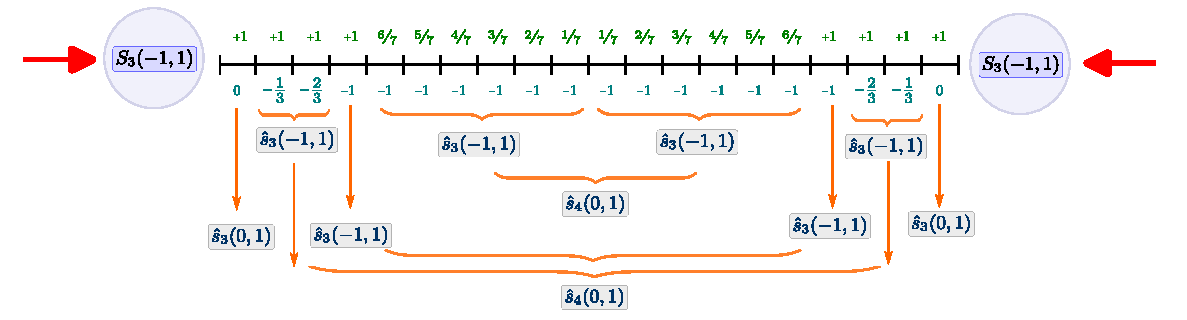
\includegraphics[width=1.0\columnwidth]{interaction-S3.pdf}
	\caption{\footnotesize{\textbf{Fusion of two $S_3$ nodes.} Fusion product of $S_3$ nodes according to their type. The red arrow represents the fusion force. The divisions represent the vorespaces of the plenum.}}
	\label{figure:4-0}
	\end{figure}
	
	\begin{multicols}{2}
	
	The process continues until a complete torus is formed. Note that our poor electron disappears completely.
	
	The $S_4$ particle cannot be matched with any particle from the standard model (spin 1, zero charge), except perhaps a massive boson like the Z boson.
	
	A calculation of the elementary mass of the Z boson gives
	\begin{equation*}
		m_{Z} = \frac{91.188 \cdot 10^6}{2^{32}} = 2.12 \cdot 10^{-2}\,eV/c²
	\end{equation*}
	
	The value is close to that obtained with the electron, so we can say it is a serious candidate.
	
	Finally, the fusions produce pseudo-electrons (which can eventually recombine into pseudo-Z bosons) and pseudo-mass.
	
	\subsubsection{from $S_5$ to $S_7$}
	
	Two $S_4$ particles merge according to the $S_2$ model to give the $S_5$ particle, a kind of super mass photon. There too, its spin of 1 and its zero charge make it a candidate for the Z boson.
	\begin{equation*}
		m_{Z} = \frac{91.188 \cdot 10^6}{2^{40}} = 8.3 \cdot 10-5\,eV/c^2
	\end{equation*}
	
	Its mass being much too low, this particle is not associable with any from the standard model.
	
	Based on the $S_3$ fusion model, two $S_5$ particles will merge into an $S_6$ particle, a "giant" $S_3$. We find the properties of the electron: negative charge and spin \R{1}{2}. The only candidate particles from the standard model could be the muon and the tauon.
	
	For the muon:
	\begin{equation*}
		m_{\mu} = \frac{105.66 \cdot 10^6} {2^{48}} = 3.7 \cdot 10^{-7}\,eV/c^2
	\end{equation*}
	
	For the tauon:
	\begin{equation*}
		m_{\tau} = \frac{1.778 \cdot 10^9}{ 2^{48}} = 6.3 \cdot 10^{-6}\,eV/c^2
	\end{equation*}
	
	Neither seems massive enough, if we consider the reference " $S_3$ is the electron."
	
	The process still produces many photons.
	
	The transition to $S_7$ gathers 7 $S_6$ nodes which this time wrap into a torus. The fusion process follows an analogous process to that of the $S_3$ fusion, due to the presence of electrical charges. The solid angle this time is an $S_6$, which is a double-helix torus. The pseudo-particles are thus fermions, of the "mass" of $S_6$. The $S_6$ nodes must also flip two by two to be able to interlock. $S_7$ is still a candidate for the muon and the tauon.
	
	For the muon:
	\begin{equation*}
		m_{\mu} = \frac{105.66 \cdot 10^6} {2^{56}} = 1.47 \cdot 10^{-9}\,eV/c^2
	\end{equation*}
	
	For the tauon:
	\begin{equation*}
		m_{\tau} = \frac{1.778 \cdot 10^9}{2^{56}} = 2.5 \cdot 10^{-9}\,eV/c^2
	\end{equation*}
	
	It would seem that this is not the case.
	\medskip
	
	The fractal growth process is complete. It has produced a hyper-massive particle $S_7$, pseudo-particles $S_6$ and $S_3$, and a quantity of photons. During the process, only two particles could have a correspondence in the standard model, namely the electron ($S_3$) and the Z boson ($S_4$), with the photon being out of competition.
	
	Is this to believe that the fractal growth law does not produce our elementary particles? It goes without saying that it does. The model must of course be placed within the framework of Big Bang thermodynamics, in the initial conditions that allowed, for example, the fusion of electrons, which is impossible under our current conditions. The temperature and kinetics of the particles are extremely high, allowing for massive nodes that are impossible to maintain under more normal conditions. It goes without saying that as soon as the temperature drops, the hyper-massive nodes can no longer hold and will simply unwind. If the initial manufacturing process had produced nothing other than these nodes, we would have a simple rebound phenomenon. But the process produced pseudo-particles that are just waiting for the passage of true particles to interact.
	\medskip
	
	Let us study what happens when the process cools down, and thus the nodes undo themselves...
	
	\subsubsection{Unwinding of $S_7$}
	
	As soon as the temperature decreases sufficiently ($T=T_{S_6}$), the $S_7$ node unwinds into 7 $S_6$ nodes. The $S_6$ are true particles, which will be able to collide with certain $S_6$ pseudo-fermions resulting from the previous fusion.
	
	We skipped a bit quickly over the application of CGC during the formation of $S_7$ when 7 $S_6$ nodes merge. The cross-section being this time an $S_6$ node, the stacking of pseudo-particles is no longer the preferred process. Indeed, this process took place because $S_2$ were topologically not capable of splitting mass or charge. This is not the case for $S_6$. As many $S_6$ pseudo-particles as there are possible fractions will therefore be created, and in double:
	
	\begin{center}
		\begin{tblr}{ccc}
			\vnode{$\hat s_6(+1,\R{1}{7})$}  & \vnode{$\hat s_6(+1,\R{2}{7})$} & \vnode{$\hat s_6(+1,\R{3}{7})$} \\
			\vnode{$\hat s_6(+1,\R{4}{7})$}  & \vnode{$\hat s_6(+1,\R{5}{7})$} & \vnode{$\hat s_6(+1,\R{6}{7})$} \\
			\vnode{$\hat s_6(-1,\R{1}{7})$}  & \vnode{$\hat s_6(-1,\R{2}{7})$} & \vnode{$\hat s_6(-1,\R{3}{7})$} \\
			\vnode{$\hat s_6(-1,\R{4}{7})$}  & \vnode{$\hat s_6(-1,\R{5}{7})$} & \vnode{$\hat s_6(-1,\R{6}{7})$} \\
			\vnode{$\hat s_6(+1,\R{+1}{3})$} & \vnode{$\hat s_6(+1,\R{+2}{3})$} &  \\
			\vnode{$\hat s_6(+1,\R{-1}{3})$} & \vnode{$\hat s_6(-1,\R{-2}{3})$} &  \\
			\vnode{$\hat s_6(+1,0)$}    & \vnode{$\hat s_6(-1,0)$}   &  \\
		\end{tblr}
	\end{center}
	
	Mass fractions are, despite everything, a topological aberration in a plenum that knows only a single massive particle. The pseudo-particles will naturally rearrange themselves to recover a nominal mass, such as 1/7+6/7, 2/7+5/7, \textit{etc}.). We thus obtain 3 massive pseudo-particles \vnode{$\hat s_6(1, 1)$} and 3 \vnode{$\hat s_6(-1,1)$}. Only the first can interact spontaneously with an \node{$S_6(-1,1)$} released by the undoing of the $S_7$ node, giving a pure mass \node{$S_6(0,1)$}. The latter can then react with the massive anti-chiral pseudo-particles to give \node{$S_6(1,1)$}.
	
	It remains to "reduce" the partially charged pseudo-particles. It suffices to associate them either with an \node{$S_6(1,1)$} particle or with an \node{$S_6(-1,1)$}. What remains in the end is:
	
	\begin{center}
		\begin{tblr}{cc}
			\node{$S_6(-1, 1)$}  & \node{$S_6(0,1)$}   \\
			\node{$S_6(\R{-1}{3},1)$} & \node{$S_6(\R{1}{3},1)$} \\
			\node{$S_6(\R{-2}{3},1)$} & \node{$S_6(\R{2}{3},1)$} \\
		\end{tblr}
	\end{center}
	
	\node{$S_6(-1, 1)$} is a stable node at this temperature and must wait for the temperature to drop to undo itself.
	
	\node{$S_6(0,1)$} is a pure mass. In a sense, it is an anomaly of the plenum, because at this temperature, only \node{$S_6(-1,1)$} is expected as a stable node. \node{$S_6(0,1)$} is too massive to spontaneously unscrew when the temperature drops and undoes the reference node \node{$S_6(-1,1)$}. It will be necessary to wait for a lower temperature to undo the excessive tightening of this node.
	
	Particles with fractional charge are also aberrations of the plenum. But before looking at how they will react, we can already note that \node{$S_6(\R{2}{3},1)$} and \node{$S_6(\R{-1}{3},1)$} are excellent candidates for the top and bottom quarks. It is very difficult to perform an energetic calculation, as we do not yet have an obvious rule, due to the partial charges. However, if we consider that the \node{$S_6(1,1)$} particle is the heaviest, then \node{$S_6(\R{2}{3},1)$} follows it immediately in terms of mass. Likewise, \node{$S_6(\R{-1}{3}, 1)$} is found to be quite far from it, and the difference in mass between the two quarks can thus find a logical explanation.
	\medskip
	
	Let us return to our charge imbalance. As with the case of fractional masses, particles with fractional charges will try to gather to recover the nominal charges of the plenum, namely $+e$ and $-e$. The top and bottom quarks will thus unite, and the only way to arrive at an integer charge is to assemble 2 tops and 1 bottom. There are several ways to assemble these 3 quarks, but the most natural, most compatible with the Ockhamite principle, is to assemble them on the $S_3(S_6)$ model. We will see later that this model is absolute and that it is found everywhere, including in atoms. The 3 double-helices will wrap, the bottom "sandwiched" in between, forming a single double-helix by the fusion of the 3 double-helices. There are thus three layers in the final double-helix. Since the charge is positive, we will call this particle a \textit{mega-proton}, because the bonding will give it a stability far superior to the sum of the unit energies. It is probable that its energy lies well beyond 100\,GeV/c². According to my research, no particles of this energy have been detected to date.
	
	Similarly, the remaining \node{$S_6(\R{-2}{3},1)$} and \node{$S_6(\R{1}{3},1)$} will merge according to the same mode, with the \node{$S_6(\R{1}{3},1)$} sandwiched between the 2 \node{$S_6(\R{-2}{3},1)$}. This particle has a high mass, a spin of \R{1}{2}, and a negative charge. It is a good candidate for the tau lepton, a \textit{mega-electron}.
	
	The remaining pure mass, \node{$S_6(0,1)$}, has a spin of \R{1}{2} and possesses no charge. It is a good candidate for the tau neutrino.
	
	\subsubsection{Unwinding of $S_6$}
	
	If the temperature continues to fall, it then reaches the unwinding temperature of $S_6$, $T_{S_5}$. \node{$S_6(-1,1)$} then unwinds classically into \node{$S_5(0,1)$}. The other previously created $S_6$ nodes are too constrained by their off-system structure and cannot unwind at this stage. An explanation for this physical impossibility is that an unwinding of a partial charge or mass cannot occur in an $S_5$ type node; it requires an analogous—self-similar—structure to transfer itself.
	
	At most, we can say that these nodes relax with the drop in temperature, making them increasingly fragile.
	
	\subsubsection{Unwinding of $S_5$}
	
	The temperature continues to drop and reaches $T_{S_4}$, the unwinding temperature of the $S_5$ node. This is the appearance of the Z boson. The previous $S_6$ nodes continue to relax, but having no nodal correspondence at this temperature, they remain bound.
	
	Between the unwinding of $S_6$ and that of $S_5$, these nodes have unwound so much that the clamping tension has dropped sufficiently to transform the previous quarks. It could be that the top quark becomes a charm quark and the bottom quark becomes a strange quark. They are still $S_6$ type structures. Visually, they are identical to their elders, but simply larger.
	
	However, the baryon $\Xi_{cc}^{++}$, recently observed by a CERN team at the LHC \cite{cern-lhcb-charmed2022}, suggests that the s quark is more likely a highly-tensioned $S_3$ than a relaxed $S_6$. Indeed, the baryon $\Xi_{cc}^{++}$ is composed of 2 charms and a down, which will only appear in the next temperature zone. Since the strange quark is heavier, there remains uncertainty about its real structure.
	
	\subsubsection{Unwinding of $S_4$}
	
	Finally, the temperature reaches $T_{S_3}$, the electronic temperature, close to the current temperature of our universe. The previous $S_4$ node releases its $S_3$ nodes and electrons reappear.
	
	This step has a huge impact on the $S_6$ currently relaxing. They finally have a self-similar structure that allows them to unwind completely. All $S_6$ transform into $S_3$. There is a kind of avalanche effect, because one $S_6$ produces $2^{24}$ $S_3$! The mega-protons and tauons, and the mega-electrons, will also reduce, producing all their $S_3$ counterparts:
	
	\begin{center}
		\begin{tblr}{cc}
			\node{$S_3(-1, 1)$}       & \node{$S_3(0,1)$}        \\
			\node{$S_3(\R{-1}{3},1)$} & \node{$S_3(\R{1}{3},1)$} \\
			\node{$S_3(\R{-2}{3},1)$} & \node{$S_3(\R{2}{3},1)$} \\
		\end{tblr}
	\end{center}
	
	The \node{$S_6(\R{-1}{3},1)$} thus becomes a d quark \node{$S_3(\R{-1}{3},1)$} and the \node{$S_6(\R{2}{3},1)$} a u quark \node{$S_3(\R{2}{3},1)$}. The remaining \node{$S_3(\R{1}{3},1)$} and \node{$S_3(\R{-2}{3},1)$}, unable to exist as such in the plenum, associate in a triplet, according to the process mentioned above, to form a particle analogous to an $S_3$ form. This is the muon lepton, with charge -e and spin \R{1}{2}. The pure mass \node{$S_3(0,1)$} is of course a candidate for the muon neutrino.
	
	\subsubsection{Final word}
	
	If we were exactly at temperature $T_{S_3}$, the process would stop there, but the temperature of the universe must currently be slightly below that. Pure mass \node{$S_3(0,1)$}, as an anomaly of the plenum, will also want to untie itself, and the only possible outcome is to untie into an analogous state, which is that of the plenum. \node{$S_3(0,1)$} will therefore tend to unwind into unit pure mass \node{$S_0(0,1)$}, that is to say, a mass vorespace. This will be our last element of the standard model: the electron neutrino.
	
	Note in passing that this step resolves the problem of the unique chirality of the neutrino. If neutrinos are "left-handed," it is because the plenum naturally rotates to the left; therefore, as a unit element of the plenum, the neutrino has no choice but to align with the rotation direction of the vorespaces.
	
	But is this the end? If the temperature were zero, then the electron neutrino would be confined in its state (we will see a possible evolution at this stage in the Big Bang model). But the temperature is rather close to $T_{S_3}$, so the electron neutrino will gather with an anti-neutrino, creating an $S_1$, which itself may eventually create an $S_2$. Being at the lower threshold of $T_{S_3}$, it is probable that no $S_2$ can transform into $S_3$.
	
	A certain amount of pure neutron mass \node{$S_0(0,1)$}, \node{$S_1(0,1)$}, and \node{$S_2(0,1)$} is thus created and gradually accumulates. This accumulation is a good candidate for dark matter. Representing 2/7 of the possible nodes of matter, by conservation of mass, it must represent 28.6\% of the total matter of the universe. This figure corresponds to current predictions—which place the amount of dark matter between 25\% and 27\%.
	
	It should be noted that by analogy with the vorespace, the neutrino is thus the natural candidate as a magnetic monopole, thereby confirming what Georges Lochak had shown. \cite{lochak2002monopole}
	\medskip
	
	Of course, three candidates are still missing. Let us deal with the $W^{\pm}$ bosons. These are clearly "impossible nodes." They have a bosonic structure—therefore a node of type $S_1$, $S_2$, or $S_4$, $S_5$—and are very heavy, thus rather a node of type $S_4$ or $S_5$. However, as they are charged, this charge makes them incompatible with the previous nodes. In reality, these bosons do not exist as such: in the standard model, they simulate the \textit{natural action of the plenum, its geometry, which imposes the relationship between the different nodes according to their charges. It is indeed an intrinsic property of the plenum, which needs no external auxiliary to manifest itself}.
	
	Finally, the Higgs boson is somewhat particular. We stopped the growth model at $S_7$. But in theory, it is possible to push the model further to create an $S_1$ "super node," built from $S_7$ units. The solid angle of coverage for each of the $S_7$ assemblies is a circle (a torus in reality) and should therefore yield a bosonic torus of spin 1. However, this process is actually impossible because fractality dictates a return to step 1 as a self-conforming element, thus with spin 0. It is through this process that the Higgs boson appears: zero charge and spin 0, with very high energy.
	
	All the elementary particles of the standard model have been reconstituted, with the exception of the $W^\pm$ bosons, which are the expression of the deep nature of the plenum.
	
	\subsubsection{Baryonic matter}
	
	It would have been a pity to stop there without beginning to introduce baryonic matter. However, this point will be further developed in the section dedicated to atomic nuclei.
	
	For reasons of stability, no knotted structure can exist in the plenum without being in equilibrium—that is, in communion with the structure of the plenum, the vorespaces. This forces any incomplete node—partially charged or partially massive—to find a way to complete its deficiency. The only means of completion is association with another partial node. As the reference node model is the vorespace, an $S_3$ state, association must favor this form, which is why partial nodes generally associate via the fusion of three partial nodes.
	
	Similarly, to regain an $S_3$ form analogy, the nodes wrap into one another around a helical axis to recover the double-helix shape. It is this shape that provides the property of the final particle, rather than the sum of the properties of its components.
	
	Indeed, when a proton forms (by the association of 2 \node{$S_3(\R{2}{3},1)$} and 1 \node{$S_3(\R{-1}{3}, 1))$}, one might think the spin value is \R{1}{2}, because it is formed of three nodes, one of which is inverted to respect the wrapping (the "screw pitch"), and that the spin is the sum of 2 spins of \R{1}{2} and one spin of \R{-1}{2}.
	
	In reality, this is false, as shown by the "proton spin crisis," because the proton's breakdown proves that the value of each internal spin contributes only about 25\% of the final total \cite{ashman1988measurement}. It is indeed the total form, of type $S_3$, that carries the main signature, just as it is the form \node{$S_x(-1,0)$} that carries the electric charge, found at the scale of the vorespace, or at the fractal scale $2^{24}$ times larger! This should close the debate on the proton spin crisis. \textit{It is the form that carries the physical characteristic, not the sum of the components.}
	
	The neutron is, of course, the other way of gathering the remaining nodes.
	
	It remains to understand why the proton and the neutron associate. This answer will come in the section on the atomic nucleus.
	
	Here is a summary table of elementary particles according to the standard model of \PQ:
	\vfill
	
	\end{multicols}
	\vspace*{-1cm}
	\begin{center}
	\begin{longtblr}[
		%theme=widecaption 
		caption={\footnotesize{\textbf{Order of appearance and structures of elementary particles}}},
		label = {tblr:5-0-2},
		]{
			colspec={Q[c,m]  Q[c,m] Q[c,m] },
			rowspec={Q[c,m]},
			row{odd}={bg=blue!10!white},
			row{1}={c,mode=text,fg=white,bg=pkcolor, cmd=\textbf}, %cmd=\textbf, blue!80!orange
			rowsep=2pt, colsep=3pt,
			vline{2-Y} = {1}{0.3pt,gray!50},
			vline{2-Y} = {2-Z}{0.3pt,gray!30},
			hline{Z} = {0.1pt,blue},
			% nombre de col début et fin qui apparaissent à chaque page
			% 1 pour le titre par exemple
			rowhead = 1, %rowfoot = 1, 
		}
		
		Temperature (decreasing)  &   Nodes                                &   Elementary particles   \\
		$T_{S_6}$                 &      \node{$S_6(\R{2}{3},1)$}           &   Top quark                 \\
		&      \node{$S_6(\R{-1}{3},1)$}          &   Bottom quark              \\
		&      $t+b+t$                            &   mega-proton (off-model) \\
		&      \node{$S_6(\R{-2}{3},1)$}+\node{$S_6(\R{1}{3},1)$}+\node{$S_6(\R{-2}{3},1)$} &   Tau (mega-electron)\\
		&      \node{$S_6(0,1)$}                  &   Tau neutrino          \\    
		$T_{S_4}$                 &      \node{$S_4(0,1)$ }                 &   Z boson                    \\
		$T_{S_3}$                 &      \node{$S_6(\R{-1}{3},1)$}+\node{$S_3(\R{2}{3},1)$}+\node{$S_3(\R{-1}{3},1))$}    &  Muon lepton\\                    
		&      \node{$S_6(\R{-1}{3},1)$}          &   d quark                    \\          
		&      \node{$S_6(\R{2}{3},1)$}           &   u quark                    \\
		&      \node{$S_3(-1,1)$}                 &   Electron                  \\                      
		&      \node{$S_3(0,1)$}                  &   Muon neutrino          \\
		< $T_{S_3}$               &      \node{$S_2(0,1)$}                  &   Dark matter                \\
		&      \node{$S_1(0,1)$}                  &   Dark matter                \\
		&      \node{$S_0(0,1)$}                  &   Electron neutrino (dark matter)  \\
		&      \node{$S_0(-1,0)$}                 &   Vorespace (off-model)  \\                    
		
	\end{longtblr}
	\end{center}
	%\end{multicols}
	
	\begin{multicols}{2}
	
	This table must be completed by the following remark: the photon is a particle apart, resulting from the rupture of the plenum, thus from a dimensional rupture (symmetry breaking). The $W^\pm$ bosons, as well as the gluon, do not exist as such, as they are expressions of the structural constraints of the plenum.
	
	\subsubsection{Conclusion}
	
	One could almost conclude the article, since the goal stated at the beginning—namely, to reconstruct the standard model of elementary particles—has been achieved. However, it would be a shame to stop in such a good way. We will show that not only is \PQ\ compatible with other physics, but we will also reconstruct an atom from the perspective of \PQ, propose a "complete" Big Bang model, and answer some of the major problems that physicists face in their respective theories.
	
	\subsection{Movement within the plenum}
	
	A response is still missing at this stage to the question: "how does a particle physically move through the plenum?". Indeed, the answer is by no means trivial.
	
	First, let us study the simplest particle, namely the neutrino. It is a massive particle that is a natural constituent of the plenum. It is governed by its laws and, while it technically forms a topological plug wherever it is located, it can move without problem. It thus screws itself naturally into a vorespace, according to the rules of the plenum, and therefore at the rhythm of the plenum. \textit{The neutrino thus travels at the speed of light.}
	
	Does this violate special relativity? No, because the neutrino is an elementary brick: it is a component of the structure.
	
	We must now focus on other particles. These are nodes, so they must move all together to respect their node shape. However, movement in the plenum occurs through self-replication. After one tick of the plenum, a particle has reconstituted itself on the next vorespace. But until it has reconstituted, the linked fused particle cannot begin its replication process. Of course, there is no question of "defusing" objects during replication, otherwise we would observe a shower of photons with every movement of a mass, which is not seen. Furthermore, the energetic cost would be such that an object would lose all its mass very quickly.
	
	It is simpler to play with the tension of the node. The outer part of the particle will move through self-replication, creating a general tension in the node. In the next step, facing the "void" of the vorespace, the next series will replicate in turn, partially relaxing the node. And so on until the last series. Then it starts again from zero. \textit{A node thus advances in the manner of a caterpillar.}
	
	Of course, the dispersion cost of the caterpillar means it is impossible for a massive particle to match the speed of light, as the caterpillar would be totally stretched during movement. Massive particles of the universe, other than neutrinos, do respect special relativity.
	
	\subsection{Forces within the framework of \PQ}
	
	\subsubsection{The force of gravity}
	
	It is useful at this stage to properly reformulate force with everything established previously. We have seen that force applies a mass phonon to the plenum according to a 7-step process in the final analysis.
	\vfill
	\end{multicols}
	
	\begin{figure}[H]
	%\captionsetup{width=5cm}
	\centering
	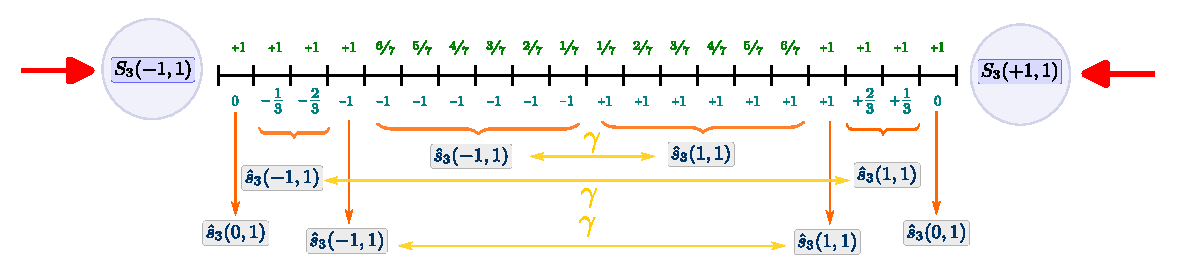
\includegraphics[width=1.0\columnwidth]{interaction-S3-antiS3.pdf}
	\caption{\footnotesize{\textbf{Fusion of two $S_3$ and anti-$S_3$ nodes.} Fusion product of an electron and a positron. The red arrow represents the fusion force. The divisions represent the vorespaces of the plenum.}}
	\label{figure:5-0}
	\end{figure}
	
	\begin{multicols}{2}
	
	The contact interface is the solid angle under which the massive particle presents itself, which is generally a form of $S_3$ or $S_6$.
	
	Depending on whether tori or $S_3$ are formed, the overlapping process differs slightly in its initial procedure, but not in its finality. When $S_2$ nodes form, they first compact into \vnode{$\hat s_3(0,1)$} before being ejected, whereas when they are \vnode{$\hat s_3(0,\R{i}{7})$} (for $i$ from 1 to 7), they are ejected as they are before recombining into \vnode{$\hat s_3(0,1)$}.
	
	Each pair of \vnode{$\hat s_3(0,1)$} on each side will merge under the pressure of gravity, transferring energy on one side to the fusion object, the photon, and on the other to the massive object to be merged. Thus, 2 photons are created, and the fusion has recovered the energy of 2 vorespaces.
	
	The energy balance is that each massive object has a fusion cost that is double from an energetic point of view: one for the object, one for the fusion.
	
	We can therefore calculate the energy of a neutrino. For example, the electron is composed of $2^{24}$ fused neutrinos, i.e.:
	\begin{equation*}
		m_{\nu_{fusion}} = \frac {0.511 \cdot 10^6} {2^{24}} = 30.46\,mEV/c²
	\end{equation*}
	
	Since the neutrino is double a vorespace, we deduce:
	\begin{equation*}
		m_{\nu} = 15.23\,meV/c²
	\end{equation*}
	
	in agreement with standard model predictions which place its mass below 0.8\,eV/c².
	
	\subsubsection{The electric force}
	
	The electric force thus concerns the phenomenon generated on the plenum in the presence of two charges. There are no purely charged particles without mass. Mass must therefore be added to the equation of the problem.
	
	The problem is actually similar to the one resolved during the approach of two masses of the same sign (\textit{cf.} figure \ref{figure:4-0}). It was necessary, to respect the torsion of the plenum, to flip a mass to adapt the chiralities.
	
	Here, opposite chiralities are consubstantial with the problem.
	
	\vnode{$\hat s_3(1,1)$} and \vnode{$\hat s_3(-1,1)$} are produced, which generate photons without the need for energetic cost. The process is inherent to the plenum.
	
	\subsection{The constants of physics in light of \PQ}
	
	\subsubsection{Time and mass}
	
	It will now be necessary to link \PQ\ to the constants of physics. By construction—by essence, one might say—\PQ\ is special relativity, and we have therefore already introduced $c$, the nominal transmission speed in the plenum at equilibrium.
	
	According to current physics, the Planck length is the minimum length below which current physics "collapses." It is the spatial limit where measurement begins. Technically, it can be seen as the spatial spread of the smallest physical object.
	
	This definition poses a problem in \PQ, because the smallest object is the neutrino, the elementary mass. If this object is the size of Planck—that is, if the vorespace is the size of Planck—then the photon travels twice the Planck size across its dimension, and thus goes half as fast as light. We are therefore forced to admit that the vorespace is not the Planck size, but half of it.
	
	There exists, therefore, \textit{de facto} an object smaller than the Planck size: the neutrino. This is the reason why a mass can travel at the speed of light without violating special relativity.
	\medskip
	
	We can now calculate some values. For example, the tick of the plenum is:
	\begin{equation*}
		\begin{split}
			t_v &= \frac {L_v}{c} = \frac{1}{2} \frac{L_p}{c} \\
			&= 1/2 \times 1.616 \cdot 10^{-35} /299 792 458 \\
			&= 2.695 \cdot 10^{-44}\,s
		\end{split}
	\end{equation*}
	
	Thus, $t_v = \R{1}{2}t_p$, which is normal, since the vorespace is 2 times smaller than the Planck length.
	
	Moreover, the mass of the bound neutrino is:
	\begin{equation*}
		m_{\nu_{bound}} = \frac {0.511 \cdot 10^6}{2^{24}} = 3.045 \cdot 10^{-2}\,eV/c^2
	\end{equation*}
	
	If the mass of the photon is indeed zero, we have, for 2 bound neutrinos, 8 "consumed" vorespaces, i.e., a ratio of 1 to 4. The mass of the neutrino is therefore 1/4 of the bound mass, i.e.:
	\begin{equation*}
		m_{\nu}= 7.6\,meV/c²
	\end{equation*}
	
	This mass is compatible with current measurements, which expect a neutrino mass below 800\,meV/c².
	
	In fact, we have a unit mass of the vorespace of half that, i.e., $m_v = 3.8\,meV/c²$.
	
	\subsubsection{The case of light: and let there be Planck's constant!}
	
	The case of light has not been fully treated until now, and its analysis will allow us to settle many details not yet addressed, such as the relationship between the photon and electric charges. The creation of the photon might lead one to believe that the photon currently used by physics is this object. It is not. Or at least, we will see that it is actually a mere superset.
	
	Indeed, if we look at things from a mechanical point of view, a photon the size of a vorespace, or even a double-vorespace, cannot easily interact with an electron, a node $2^{24}$ times larger. It would have to hit it according to a complicated process to justify an interaction. It is much simpler to postulate that the photon interacting with the electron is an object of similar size: it can then wrap naturally, like the photon on the vorespace, since the electron is just a giant vorespace. This is fractal reality!
	
	The photon will therefore seek to adopt the node of the plenum that resembles it and is stable at the scale of the plenum. This is not an $S_3$ node, since the photon has a spin of 1. By construction, it is an $S_2$ node. This is exactly the object sought, because the size of the $S_2$ node allows for a perfect fit around the $S_3$ node, the $S_3$ node being nothing more than an $S_2$ node "elevated to the higher dimension."
	
	We could stop there, say the process is consubstantial with the plenum, and accept it. It may be interesting to justify the construction of this object.
	
	Indeed, until now, we have assembled two neutrinos via the force of gravity. How to assemble two photons, given that they are pure phases? Precisely through phase. The photon has a natural phase rotation of $2\pi/7$. Two photons together can only "be in phase" by adjusting their phase! The two photons then become a single double photon.
	
	Furthermore, we have only a single process for developing our final object: the fractal process of \PQ. The photon must follow it and create first an $S_1$ node before reaching the $S_2$ node. This process poses a technical problem: an $S_1$ node is a "circle" of photons. How to bend photons?
	
	Fortunately, gravity comes to save the rectilinear alignment of photons. The photon is a \textit{phonic surfer}, and as soon as it encounters a mass, it follows the valley of negentropy: the presence of a neutrino, with its heptagonal phonon, will force the rectilinear groups of photons to "orbit" around the neutrino and assemble. The $S_1$ node then takes birth around the neutrino. The next step is to assemble 7 nodes together. This is easy, as two $S_1$ nodes offset by $2\pi/7$ fit together perfectly. But since the space is already occupied on a vorespace, the first circle of photons must be shifted by a half-vorespace, according to the organization of the DNA strands of the plenum. There are, of course, 7 shifts before closing a complete wrapping. Then, one must repeat 7 times with the previous set: the first set of $2^7$ photons is ready to meet a counterpart to form the final object.
	
	The fusion vector must evolve at this stage, as the neutrino does not have the necessary waveform to move the new object in two different space directions. It then hands over to the electron. The latter, of $S_3$ form, produces a more complex heptagonal wave along two perpendicular axes. One $S_1$ node will take the direction of one axis (still surfing phonically) and the second the other, until they meet: the object is then created! It is an $S_2$ node.
	\medskip
	
	We can show that this node is the photon of modern physics by calculating its wavelength.
	
	This node is indeed a fractal image of the elementary photon. The latter has a wavelength equal to the Planck length $L_p$. The fractal length, having passed through two dimensions, will thus be $7\times 7$ times the Planck length.
	
	One must subtract from this length the thickness of the conformal photon, because the latter is no longer a simple phase, having grown by fractality twice: each fractal thickness must therefore be removed, namely 1 for the first and 7 for the second. The wavelength of the homologous photon is therefore $41 \cdot L_p$.
	\begin{equation*}
		\lambda_{\gamma} = 41 \cdot L_p = 41 \cdot 1.616255 \cdot 10^{-34} = 6.6266 \cdot 10^{-34}\,m
	\end{equation*}
	
	\textbf{This is exactly Planck's constant!}
	\medskip
	
	The formula $E=h\nu$ is therefore the minimum energy packet for one period cycle, i.e., a frequency of 1. This is "E=h", i.e., $E=6.6 \cdot 10^{-34}\,J$.
	\medskip
	
	As it is an $S_2$ type node, it is composed of $2^{15}$ elementary photons (there are 2 photons per assembled vorespace), so we can calculate the mass of the latter:
	\begin{equation*}
		m_{\gamma_{el}} = \frac {E_{unit}} {2^{15}} = 1.91 \cdot 10^{-38}\,J = 1.65 \cdot 10^{-57}\,eV/c²
	\end{equation*}
	
	\textit{The elementary photon thus does have a mass, contrary to what the standard model of physics states.} However, the latter is not at all absurd, in the sense that this mass is so small that considering it as zero is an approximation close to reality.
	
	The fact that the photon has a mass of this magnitude has little impact on physics, because:
	
	\begin{itemize}
		\item it is totally negligible in binding energy;
		\item it is not detectable even at the scale of the universe, because its half-wavelength is on the scale of half the universe (\textit{cf}. the Big Bang model).
	\end{itemize}
	
	Nonetheless, the photon does have a mass, as also predicted by de Broglie, who calculated it around $10^{-61}\,eV/c²$\cite{debroglie1956tentative}. The cosmological limit also suggests a value around $10^{-62}$.
	\medskip
	
	The conclusion imposes itself: the speed of the photon cannot be rigorously equal to "that of light." The difference between these speeds is so small that it is not measurable. It would be fascinating to find an experiment allowing it to be highlighted. The simplest would be to find an emission source located at the opposite side of our position in the universe and measure the time difference upon arrival. But disregarding the contingencies encountered along the way is a major challenge!
	
	\textit{Stricto sensu}, it would therefore be necessary to rename the speed of light as the plenum speed $v_p$, while henceforth considering the ratio $v_p/c$ constant.
	
	\subsubsection{The electromagnetic interaction}
	
	The consequences of the foregoing must be studied. From now on, the homologous photon will be called the "photon," and the basic photon will be called the "elementary photon."
	
	The photon is adapted to the process of wrapping around a dimensionally homologous $S_3$ node. This is the case for the electron, which is the homologue of the vorespace but is composed of neutrinos.
	
	However, while the elementary photon "passes through" the vorespace without flinching—though strictly speaking, we must now account for the fact that this is not rigorously exact—this is not the case for the photon with the electron. Indeed, while the electron is the conformal image of the vorespace, it is not so structurally: the electron is composed of neutrinos, and thus of mass. It must have strictly the structure of the vorespace, and therefore be an \node{$S_3(-1,0)$} node to possess the property of charge, but it is massive and thus has a mass: it is an \node{$S_3(-1,1)$} node.
	
	Since it is an \node{$S_3(-1,1)$} node, it has at least one mobilized helix (the distribution of roles between the helices will be justified at the end of this chapter), and it is indeed a turbine around which the photon can wrap. But even if the final width is always the maximum width, the blade is still very slightly deformed by the mass—one can see it as flattened by gravity—and the photon will hit this final stage without being able to finish its wrapping, as it did for a vorespace. In a sense, the photon no longer has enough room to pass and crashes against the wall of the blade.
	
	All the photon's energy is then transferred in 7 steps to the electron. The electron is a stable node that cannot modify its structure without violent transformation energy. As the photon's energy is too low to impact the \textit{in se} structure of the node, it must disperse otherwise: unable to increase its rotation speed, the electron will transfer this energy into its translation speed, its exergy, by pure conservation of energy. The photon's angular momentum is transformed into translational momentum. This is Noether's theorem.
	
	The process is not without consequence: the transmission occurs at the photon's frequency, i.e., $1/h$, which is $1.6 \cdot 10^{27}\,Hz$, or $6.6 \cdot 10^{-34}$ seconds. The electron accelerates during this brief instant to change its speed, and thus its position. At the microscopic scale, because physics measures characteristics with a wavelength on the order of the photon, \textit{it gives the impression of disappearing and reappearing in another location, having changed speed at the new location.} In reality, the law of action-reaction has been scrupulously respected: consequently, the fundamental principle of dynamics has been as well.
	
	However, \textit{this principle is now quantized}. Acceleration, like deceleration, can only occur by photon quanta, according to a time quantum. At the microscopic scale, the phenomenon is already beyond the sensitivity of our experimental means.
	
	By conservation of energy, the decelerating electron must yield a quantum of energy equivalent to that of a photon (for a one-unit quantum deceleration). A slowing electron therefore emits a photon. Here again, it changes position "instantaneously" according to our measuring devices. The mechanical process by which the photon appears in this context should be studied. It is likely an inverse phenomenon of the sonic boom: as it slows down, the wave in front of the object loses pressure and relaxes: the photon is the phonic "boom" of the "phonon wall."
	
	In any case, this process will be enlightening to illustrate part of the atomic model that will be developed later.
	
	Finally, it is because the last screw thread blocks the passage of the photon that the interaction between the photon and the electron is inevitable.
	
	If we take a mass equivalent to the electron, hence an \node{$S_3(0,1)$} node, then the photon will not hit the last step, because the node constraint, distributing entropy between states 0 through 64, will set the two internal screws in motion, transforming the blades and leaving enough room for the photon to pass. Paradoxically, the massive $S_3$ node plays the role of the vorespace at the fractal scale. This paradox is explained by the fact that the plenum is no longer quite a fractal structure, as its initial energy was not sufficient to preserve all fractal properties (\textit{cf.} the Big Bang model). Technically, the photon has very little chance of passing through matter other than pure neutrino, as the mass wave should deflect it.
	
	\textit{The photon is thus indeed the vector of the electromagnetic interaction.}
	
	Finally, we have a fairly detailed mapping of the electron. It is an $S_3$ node with a dimension of the photon's half-wavelength along its double screw thread, thus 42 vorespaces, or 21 Planck lengths. The diameter of the "screw head" corresponds to that of the photon circle, i.e., a perimeter of $2^7$ elementary photons of one Planck length each, giving a diameter of $2^7 \cdot L_p/\pi$.
	
	We must now "dress" the electron with the thickness of its dimension, multiplying each dimension by $2^{16}$. The external dimensions of the electron are thus $2^{23} \cdot L_p/\pi$ for the head diameter, or $4.3 \cdot 10^{-29}\,m$.
	
	The electron is therefore a top four times wider than it is high. It is a "very flat" turbine.
	
	\subsubsection{De Broglie's formula}
	
	A consequence of the fact that an object's displacement is quantized by energy quanta will allow us to arrive at de Broglie's famous formula.
	
	We must return to the way an object moves: by caterpillar-like self-replication. An object of characteristic length $L$ will therefore move at a characteristic time of $L/c$.
	
	As the object itself generates a unique wave characterizing it, by analogy, the wave also moves at this characteristic time. Since the wave has a different characteristic length, its wavelength $\lambda$, its own characteristic time is $\lambda/c$. The wavelength is therefore equal to the characteristic length of the physical object, which is not surprising, since it is this characteristic that imprints its signature into the plenum.
	
	Now we know that to move the object by one momentum quantum, it needs a quantum of energy corresponding to $h$. As the object has a characteristic dimension of $\lambda$, it needs $\lambda/h$ quanta to determine its momentum,
	
	thus
	\begin{equation*}
		p = \frac {h}{\lambda}
	\end{equation*}
	
	This reasoning is close to that of de Broglie, who "synchronized" the phase and group velocities between the quantum object (an electron he considered indeformable) and its pilot-wave—an idea he considered the most important of all his scientific discoveries.\cite{debroglie1963etude}
	
	\subsubsection{The fine-structure constant}
	
	In reality, the photon only just fails to pass when it attempts to cross an electron. The difference in thickness that protrudes from the wrapping is very small: it is worth about 7 thousandths of the whole. This is obviously $\alpha$, the fine-structure constant\footnote{the importance of which is such that the author chose to number the different versions of this document according to the decimals of this constant.}. Before looking further into how to determine it, let us observe what happens at the plenum scale when an elementary photon crosses a vorespace.
	
	The latter, as a topological aberration, is forced to skip every other step of the vorespace, meaning it needs 2 vorespaces to fully unroll.
	
	Technically, the elementary light photon slides at speed $c$ (at least, to a very reasonable approximation), following the shapes of the vorespace, even if it skips one in two. These shapes depend on two parameters: the width of the blade—"its surface"—and its inclination, the former relating to magnetic charge and the latter to electric charge. There is therefore a direct relationship linking the 3 characteristics.
	
	Let $\epsilon$ be the characteristic of inclination and $\mu$ that of the width of the inclined blade. $\epsilon$ reflects a linear charge (a charge per length), while $\mu$ reflects a magnetic field (a unit of magnetic field, which corresponds to a length traveled by a charge flux, thus charges per unit of time). The product of the nodes gives the inverse of a speed squared. We can therefore link these three quantities by recovering the famous formula:
	\begin{equation*}
		c^2 = \frac{1} {\epsilon \cdot \mu}
	\end{equation*}
	
	Thus, by alignment with current physics,
	\begin{equation*}
		\left\{
		\begin{split}
			\epsilon &= \epsilon_0 \\
			\mu      &= \mu_0
		\end{split}
		\right.
	\end{equation*}
	
	We can finally give meaning to an absurdity of physics which claims without blinking that a vacuum exists$\ldots$ and that it has a non-zero permittivity.
	
	Either the permittivity is zero and the vacuum is indeed empty, or the permittivity is non-zero and the vacuum is not empty. Fortunately, the plenum is here to save the ontology of permittivity!
	\medskip
	
	At the level of the vorespace, we now have a way to measure the elementary photonic flux by linking the elementary photon speed to the electromagnetic characteristics of the vorespace.
	
	This mechanism must now be transposed to the photon and the electron.
	
	In reality, one might think that since the structures of the vorespace and the electron are identical, the mechanical interlocking effects would be identical. This is correct. With one exception: the electron is not self-similar to the vorespace, but to the neutrino. We must therefore carefully compare the vorespace and the neutrino to sense what occurs differently between the two.
	
	Until now, we have not focused much on the effective role of each of the helices in the vorespace or neutrino "turbine." In fact, their roles are specific: one deals exclusively with charge, while the other deals with mass. The fact that they are constrained together explains the coupled nature of these interactions.
	
	On the other hand, the plenum constraint means that both the vorespace and the neutrino must fit into the system, thus \textit{always having a rotation speed compatible with their neighbors}. Now, we have shown that the speed of the neutrino was double that of the vorespace. Technically, if this were strictly the case, the neutrino could not fit into the plenum without making everything explode!
	
	The Occamian solution consists of using the other helix, the charge helix, to act in place of the mass helix. Since the helices can have independent rotation, this is possible: we thus have one rotation for mass and one for interlocking, thanks to the charge helix, which must rotate at the speed of the vorespace, i.e., at speed $\omega_v$.
	
	Since the vorespace rotates in a levorotatory (left-handed) direction, the only solution for the neutrino's mass helix is to rotate in the other direction. To obtain an average of $(-)2 \omega_v$, it must itself rotate at $(+) 3 \omega_v$.
	
	We can extract a general property of the plenum from this observation:
	
	\begin{mybox}[breakable,colback=blue!10, colbacktitle=pkcolor]{Property}
		The composition of the rotational movements of the double-helices of a vorespace or a neutrino must always provide at least one unit rotation in the levorotatory direction for stationary states.
	\end{mybox}
	\medskip
	
	We can then construct a table of the properties of each helix according to the states of the vorespace and the neutrino:
	\vspace*{-0.5cm}
	\begin{center}
		\begin{longtblr}[
			%theme=widecaption 
			caption={\footnotesize{\textbf{Relative rotation speed of the vorespace and neutrino helices}}},
			label = {tblr:7-0},
			]{
				colspec={Q[c,m]  Q[c,m] Q[c,m] Q[c,m] Q[c,m]},
				rowspec={Q[c,m]},
				row{odd}={bg=blue!10!white},
				row{1-2}={c,mode=text,fg=white,bg=pkcolor, cmd=\textbf}, %cmd=\textbf, blue!80!orange
				rowsep=2pt, colsep=3pt,
				vline{2-Y} = {1}{0.3pt,gray!50},
				vline{2-Y} = {2-Z}{0.3pt,gray!30},
				hline{Z} = {0.1pt,blue},
				rowhead = 1, 
			}
			\SetCell[r=2]{c} States  & \SetCell[c=2]{c} Helix 1 (charge) && \SetCell[c=2]{c} Helix 2 (mass) \\
			& vorespace                           & neutrino              & vorespace    & neutrino           \\
			0-20            &    -1                                &    -1                 &     0        &   0                \\
			21-42            &  \Ru{-}{2}{3}{} to \Ru{-}{1}{3}{} &    -1                 &    \Ru{-}{1}{7}{} to \Ru{-}{6}{7}{}   &  \Ru{}{3}{7}{} to \Ru{}{18}{7}{}     \\
			43-45            &    0       &    -1                 &     -1        &   +3                \\    
		\end{longtblr}
	\end{center}
	
	We notice something strange. It is not possible to initiate a rotation at $-1$ for the neutrino's mass helix, otherwise the variation in steps of 7 up to the $+3$ rotation would pass through zero, which has no physical meaning (there would be a chirality inversion during states 21 to 42). Only its charge helix must carry this value. But since it also carries it in the end, its rotation speed remains constant!
	
	This oddity should not be interpreted beyond the domain of existence of the neutrino. The neutrino is the \node{$S_0(0,1)$} node, i.e., the complete state from 0 to 64. The fact that it has an apparent charge in its state 0 to 20 comes from the fact that the neutrino was not born from nothing, but from the "screwing" of the vorespace (\textit{cf.} the Big Bang model). The electric charge disappears as soon as the energy is distributed over the rest of the states, because only the \node{$S_0(-1,0)$} structure carries the characteristic of the electric charge $-e$.
	
	On the other hand, one must understand \textit{how} the magnetism—or mass—of the neutrino is built. The neutrino is a more tightly screwed vorespace, but it remains a vorespace. Its incorporation into the plenum leaves it little choice for its shape: it must topologically conform to its neighboring vorespaces. Clearly, its blade surfaces cannot differ from those of its neighbors: the only freedom left to the neutrino is in the \textit{thickness} of the blade. It thus exploits all possible thickness, which freezes the overall shape. By leaving only a thin space for interlocking, the thick blade occupies all the rest of the volume, leaving no freedom of movement to the blade. In particular, it can no longer tilt: consequently, its charge remains constant. This constraint thus explains the constant value of the neutrino's apparent charge.
	
	We thus observe a notable difference between the functioning of the helices of each object:
	%\vfill
	
	\begin{center}
		\begin{tikzpicture}
			\begin{axis}[
				width=\columnwidth,
				height=0.55\columnwidth,
				xlabel={Mass (in 1/7 steps)},
				ylabel={Relative speed},
				title={Neutrino-vorespace mass competition},
				xmajorgrids=true,
				ymajorgrids=true,
				grid style=dashed,
				ymin=-1.5,
				ymax=3.5,
				xlabel style={font=\small},
				ylabel style={font=\small},
				title style={font=\bfseries},
				tick label style={font=\small},
				legend pos=north west,
				]
				
				\addplot[
				color=blue,
				thick,
				mark=*, 
				mark size=1.5pt,
				] coordinates {
					(0,0)
					(3,3/7)
					(6,6/7)
					(9,9/7)
					(12,12/7)
					(15,15/7)
					(18,18/7)
					(21,21/7)
				};
				\addlegendentry{neutrino}
				\addplot[
				color=red,
				thick,
				mark=*, 
				mark size=1.5pt,
				] coordinates {
					(0,0)
					(3,-1/7)
					(6,-2/7)
					(9,-3/7)
					(12,-4/7)
					(15,-5/7)
					(18,-6/7)
					(21,-7/7)
				};   
				\addlegendentry{vorespace}
				
			\end{axis}
		\end{tikzpicture}
	\end{center}
	
	\begin{center}
		\begin{tikzpicture}
			\begin{axis}[
				width=\columnwidth,
				height=0.55\columnwidth,
				xlabel={Mass (in 1/3 steps)},
				title={Neutrino-vorespace charge competition},
				xmajorgrids=true,
				ymajorgrids=true,
				grid style=dashed,
				ymin=-2.0,
				ymax=1.0,
				xlabel style={font=\small},
				ylabel style={font=\small},
				title style={font=\bfseries},
				tick label style={font=\small},
				legend pos=north west,
				]
				
				\addplot[
				color=blue,
				thick,
				mark=*, 
				mark size=1.5pt,
				] coordinates {
					(0,-1)
					(7/7,-1)
					(14/7,-1)
					(21/7,-1)
				};
				\addlegendentry{neutrino}
				\addplot[
				color=red,
				thick,
				mark=*, 
				mark size=1.5pt,
				] coordinates {
					(0,-1)
					(7/7,-2/3)
					(14/7,-1/3)
					(21/7,0)
				};   
				\addlegendentry{vorespace}
				
			\end{axis}
		\end{tikzpicture}
	\end{center}
	
	Since a photon is an entropic revealer, it will be sensitive to the disparity of the internal states of each object and will not react in the same way depending on the states. It will cross the vorespace but will be blocked in the electron. The difference between the two is minimal—it is the fine-structure constant $\alpha$—but sufficient to change the rules of the game for the photon's interaction with $S_3$ type nodes.
	
	Now, mass is dual with the magnetic field: it is the flux $\Phi$ of electromagnetism. We can therefore see the distribution of mass values as a dual distribution of magnetic charge values of the associated monopole. By normalizing the charges to positive values, we have:
	
	\begin{center}
		\begin{tikzpicture}
			\begin{axis}[
				width=\columnwidth,
				height=0.55\columnwidth,
				xmin=0, xmax=1.05,
				ymin=0, ymax=1.15,
				grid style=dashed,
				title={Vorespace: electric charge vs magnetic flux},
				grid=major,
				legend pos=north west,
				legend style={font=\tiny},
				title style={font=\bfseries\small},
				xtick={1/7,2/7,3/7,4/7,5/7,6/7,7/7},
				xticklabels={
					\( \frac{1}{7} \), \( \frac{2}{7} \), \( \frac{3}{7} \), 
					\( \frac{4}{7} \), \( \frac{5}{7} \), \( \frac{6}{7} \), \( \frac{7}{7} \)
				},
				xticklabel style={font=\small},
				ytick={1/3, 2/3, 3/3},
				yticklabels={
					\( \frac{1}{3} \), \( \frac{2}{3} \), \( \frac{3}{3} \), 
				},
				yticklabel style={font=\small}, 
				]
				\addplot+[ybar, bar width=1/3, fill=blue!40, draw=blue!70, thick, opacity=0.75] 
				coordinates {
					(1/6,  1)   
					(1/2,  2/3)   
					(5/6,  1/3)     
				};
				\addplot+[ybar, bar width=1/7, fill=red!40, draw=red!70, thick, opacity=0.55] 
				coordinates {
					(1/14, 1/7)
					(3/14, 2/7)
					(5/14, 3/7)
					(7/14, 4/7)
					(9/14, 5/7)
					(11/14,6/7)
					(13/14,1)
				};
				\legend{electric charge, magnetic flux};
				\node[color=red] at (2/28, 0.06) {\R{1}{7}};
				\node[color=red] at (6/28, 0.06) {\R{2}{7}};
				\node[color=red] at (10/28, 0.06) {\R{3}{7}};
				\node[color=red] at (14/28, 0.06) {\R{4}{7}};
				\node[color=red] at (18/28, 0.06) {\R{5}{7}};
				\node[color=red] at (22/28, 0.06) {\R{6}{7}};
				\node[color=red] at (26/28, 0.06) {\R{7}{7}};
				\node[color=blue] at (0.2, 0.4) {1};
				\node[color=blue] at (0.5, 0.4) {\R{2}{3}};
				\node[color=blue] at (0.85, 0.21) {\R{1}{3}};
			\end{axis}
		\end{tikzpicture}
	\end{center}
	
	\begin{center}
		\begin{tikzpicture}
			\begin{axis}[
				width=\columnwidth,
				height=0.55\columnwidth,
				xmin=0, xmax=1.05,
				ymin=0, ymax=3.15,
				grid style=dashed,
				title={Neutrino: electric charge vs magnetic flux},
				grid=major,
				legend pos=north west,
				legend style={font=\tiny},
				title style={font=\bfseries\small},
				xtick={1/7,2/7,3/7,4/7,5/7,6/7,7/7},
				xticklabels={
					\( \frac{1}{7} \), \( \frac{2}{7} \), \( \frac{3}{7} \), 
					\( \frac{4}{7} \), \( \frac{5}{7} \), \( \frac{6}{7} \), \( \frac{7}{7} \)
				},
				xticklabel style={font=\small},
				]
				\addplot+[ybar, bar width=1/3, fill=blue!40, draw=blue!70, thick, opacity=0.75] 
				coordinates {
					(1/6,  1)   
					(1/2,  1)   
					(5/6,  1)     
				};
				
				\addplot+[ybar, bar width=1/7, fill=red!40, draw=red!70, thick, opacity=0.45] 
				coordinates {
					(1/14, 3/7)
					(3/14, 6/7)
					(5/14, 9/7)
					(7/14, 12/7)
					(9/14, 15/7)
					(11/14,18/7)
					(13/14,21/7)
				};
				\legend{electric charge, magnetic flux};
				\node[color=red] at (2/28, 0.15) {\R{3}{7}};
				\node[color=red] at (6/28, 0.15) {\R{6}{7}};
				\node[color=red] at (10/28, 0.15) {\R{9}{7}};
				\node[color=red] at (14/28, 0.15) {\R{12}{7}};
				\node[color=red] at (18/28, 0.15) {\R{15}{7}};
				\node[color=red] at (22/28, 0.15) {\R{18}{7}};
				\node[color=red] at (26/28, 0.15) {\R{21}{7}};    
			\end{axis}
		\end{tikzpicture}
	\end{center}
	
	For the vorespace, the magnetic charge is induced: it is the result of the presence of an electric charge. Conversely, for the neutrino, the magnetic charge is intrinsic and the electric charge is induced. The neutrino is the only true magnetic monopole\footnote{A new approach to capturing neutrinos would be to deflect them in a magnetic field.}.
	
	It is not necessary, as with Dirac's magnetic monopole, to invent some "Dirac string" to describe the monopole's field, because the charge (magnetic) phonon, in every respect equivalent to the mass phonon, fully describes the field.
	
	Here, the flux varies by whole steps. We thus have:
	
	\begin{equation*}
		\Phi_m = \sum_{i=1}^{7} \vec{B_i} \cdot \vec{S_i} = \mu_0 q_m
	\end{equation*}
	thus
	\begin{equation*}
		B_i S_i = \mu_0 q_{m_i}
	\end{equation*}
	
	Now, the blade surfaces vary proportionally according to a ratio of \R{1}{7}:
	\begin{equation*}
		S_i = \frac{i}{7} S_0 = \frac{i}{7} \pi \frac{L_p^2}{2}
	\end{equation*}
	
	hence
	\begin{equation*}
		q_{m_i} \mu_0 = \frac{i}{7} B_i S_0
	\end{equation*}
	
	Thus
	\begin{equation*}
		\left\{
		\begin{split}
			\mu_0  &\propto S_0  \\ 
			q_{m_i}&\propto \frac{i}{7} B_i 
		\end{split}
		\right.
	\end{equation*}
	
	The magnetic permeability is indeed proportional to the blade surface, and the magnetic charge is quantized. Unsurprisingly, we recover Dirac's quantization of magnetic charge, the measurements of the quantum Hall effect \cite{klitzing1980new}, and the solution found is close to the Chern-Simons soliton \cite{jackiw1990solitons}.
	
	\begin{center}
		\begin{tikzpicture}
			\begin{axis}[
				width=\columnwidth,          % <-- exact page width
				height=0.95\columnwidth,     % proportional height
				xmin=0, xmax=1.05,
				ymin=-1.5, ymax=3.15,
				grid style=dashed,
				%xlabel={Position \( x \)},
				%ylabel={Height},
				title={Vorespace-Neutrino Competition},
				grid=major,
				legend pos=north west,
				legend style={font=\tiny},
				title style={font=\bfseries\small},
				xtick={1/7,2/7,1/3,3/7,4/7,2/3,5/7,6/7,7/7},
				xticklabels={
					\( \frac{1}{7} \), \( \frac{2}{7} \), \( \frac{2}{3} \), \( \frac{3}{7} \), 
					\( \frac{4}{7} \), \( \frac{2}{3} \), \( \frac{5}{7} \), \( \frac{6}{7} \), 
					\( \frac{7}{7} \)
				},
				xticklabel style={font=\small},
				ytick={-1, -2/3, -1/3, 0, 1, 2, 3},
				yticklabels={
					\( -1 \),     \( \Ru{-}{2}{3}{} \), \( \Ru{-}{1}{3}{} \),
					\( 0 \),  \( 1 \), \( 2 \), \( 3 \),
				},
				yticklabel style={font=\small},    
				]
				% ==================== Series 1/3: wide bars (width = 1/3) ====================
				\addplot+[ybar, bar width=1/3, fill=blue!20, draw=blue!70, thick, opacity=0.5] 
				coordinates {
					(1/6,  -1)   % center of the first bar
					(1/2,  -1)   % center of the second bar
					(5/6,  -1)     % center of the third bar            
				};
				\addplot+[ybar, bar width=1/3, fill=blue!40, draw=blue!70, thick, opacity=0.5] 
				coordinates {
					(1/6,  -1)   % center of the first bar
					(1/2,  -2/3)   % center of the second bar
					(5/6,  -1/3)     % center of the third bar
				};
				% ==================== Series 1/7: narrow bars (width = 1/7) ====================
				\addplot+[ybar, bar width=1/7, fill=red!40, draw=red!70, thick, opacity=0.45] 
				coordinates {
					(1/14, 3/7)
					(3/14, 6/7)
					(5/14, 9/7)
					(7/14, 12/7)
					(9/14, 15/7)
					(11/14,18/7)
					(13/14,21/7)
				};
				\node[color=red] at (2/28, 0.3) {\R{3}{7}};
				\node[color=red] at (6/28, 0.6) {\R{6}{7}};
				\node[color=red] at (10/28, 1.1) {\R{9}{7}};
				\node[color=red] at (14/28, 1.5) {\R{12}{7}};
				\node[color=red] at (18/28, 1.9) {\R{15}{7}};
				\node[color=red] at (22/28, 2.3) {\R{18}{7}};
				\node[color=red] at (26/28, 2.8) {\R{21}{7}};    
				% == vorespace ==
				\addplot+[ybar, bar width=1/7, fill=red!40, draw=red!70, thick, opacity=0.55] 
				coordinates {
					(1/14, 1/7)
					(3/14, 2/7)
					(5/14, 3/7)
					(7/14, 4/7)
					(9/14, 5/7)
					(11/14,6/7)
					(13/14,1)
				};
				\legend{vorespace electric charge, neutrino electric charge, vorespace magnetic flux, neutrino magnetic flux, };
				\node[color=red] at (2/28, 0.08) {\R{1}{7}};
				\node[color=red] at (6/28, 0.1) {\R{2}{7}};
				\node[color=red] at (10/28, 0.1) {\R{3}{7}};
				\node[color=red] at (14/28, 0.1) {\R{4}{7}};
				\node[color=red] at (18/28, 0.1) {\R{5}{7}};
				\node[color=red] at (22/28, 0.1) {\R{6}{7}};
				\node[color=red] at (26/28, 0.1) {\R{7}{7}};
				\node[color=blue] at (0.2, -0.4) {1};
				\node[color=blue] at (0.5, -0.4) {\R{2}{3}};
				\node[color=blue] at (0.85, -0.21) {\R{1}{3}};
			\end{axis}
		\end{tikzpicture}
	\end{center}
	
	How can we now determine the fine-structure constant? We note two unsettling facts. First, the value of this constant is surprisingly close to the neutrino mass ($7.2 \cdot 10^{-3}$ vs $7.6 \cdot 10^{-3}$). Furthermore, the fine-structure "constant" is not constant. It varies logarithmically, increasing for the Z boson \cite{workman2022review}. If we extrapolate the experimental measurements of the electron and Z boson constants\footnote{Taking $\alpha_{e^-}=7.297 \cdot 10^{-3}$ and $\alpha_{Z}=7.815 \cdot 10^{-3}$, we obtain the line $y=6.475 \cdot 10^{-5}\log_2{x}+5.743 \cdot 10^{-3}$, where $\log_2$ is the base-2 logarithm.} by plotting a logarithmic curve, we obtain:
	
	\begin{center}
		\begin{tikzpicture}
			\begin{axis}[
				xmode=log,
				log basis x=2,                  % log scale in base 2
				xmin=2^0, xmax=2^36,           % x range
				ymin=0.0055, ymax=0.0082,
				xlabel={Nodes},
				ylabel={},
				title={Fine-Structure Constants\\ (logarithmic scale)},
				grid=major,
				xmajorgrids=true,
				ymajorgrids=true,
				grid style=dashed,
				title style={align=center, font=\bfseries},
				width=0.95\columnwidth,          % <-- exact page width
				height=0.55\columnwidth,     % proportional height
				xtick={2^0, 2^8, 2^16, 2^24, 2^32, 2^36},
				xticklabels={
					\(\underset{neutrino}{1}\), \(8\), \(16\), 
					\(\underset{electron}{24}\), \(\underset{Z\ boson}{32}\), \(36\),
				},
				xticklabel style={font=\small},
				ytick={ 0.005, 0.006, 0.007, 0.008},
				yticklabels={
					\(0.005\), \(0.006\), 
					\(0.007\), \(0.008\),
				},
				yticklabel style={font=\small},
				scaled y ticks=false,
				]
				\addplot[blue, thick, domain=2^0:2^32] 
				{6.25e-5 * log2(x) + 0.0058};
				\addplot[blue, only marks, mark=*, mark size=1.5pt] 
				coordinates {
					(2^0, {0.0000625 * log2(2^0) + 0.0058})
					(2^8, {0.0000625 * log2(2^8) + 0.0058})
					(2^16, {0.0000625 * log2(2^16) + 0.0058})
					(2^24, {0.0000625 * log2(2^24) + 0.0058})
					(2^32, {0.0000625 * log2(2^32) + 0.0058})
				};
			\end{axis}
		\end{tikzpicture}
	\end{center}
	
	There is thus one constant per node of the plenum (with the neutrino constant being approximately $5.743 \cdot 10^{-3}$, or roughly $1/174$), which is not extraordinary in itself, as the constant measures the effect of mass (or magnetism) of a node's constituents relative to the vorespace model (which is only electrically charged). That the effect follows a logarithmic law is therefore intrinsic to \PQ.
	
	Let us look at how these constants evolve by calculating their approximate values from the experimentally determined line.
	
	%\vspace*{-0.5cm}
	\begin{center}
		\begin{longtblr}[
			caption={\footnotesize{\textbf{Calculation of approximate values of fine-structure constants}}},
			label = {tblr:5-0-3},
			]{
				colspec={Q[c,m]  Q[2.2cm,c,m] Q[3.5cm,c,m] },
				rowspec={Q[c,m]},
				row{odd}={bg=blue!10!white},
				row{1}={c,mode=text,fg=white,bg=pkcolor, cmd=\textbf},
				rowsep=2pt, colsep=3pt,
				vline{2-Y} = {1}{0.3pt,gray!50},
				vline{2-Y} = {2-Z}{0.3pt,gray!30},
				hline{Z} = {0.1pt,blue},
				rowhead = 1, 
			}        
			Nodes  &   $\alpha$               &  Ratio (approximate)   \\
			1    & 5.743$\cdot 10^{-3}$     &      1/174                  \\
			8    & 6.261$\cdot 10^{-3}$     &      1/160                  \\ 
			16    & 6.779$\cdot 10^{-3}$     &      1/148                  \\ 
			24    & 7.297$\cdot 10^{-3}$     &      1/137                  \\
			32    & 7.815$\cdot 10^{-3}$     &      1/125                  \\
			40    & 8.333$\cdot 10^{-3}$     &      1/120                  \\
			48    & 8.851$\cdot 10^{-3}$     &      1/113                  \\
			56    & 9.369$\cdot 10^{-3}$     &      1/107                  \\
			64    & 9.887$\cdot 10^{-3}$     &      1/101                  \\          
		\end{longtblr}
	\end{center}
	
	We "feel" therefore that there exists a logarithmic construction law based on $2^8$, and we also "feel" that this law acts fractally, first within the node, then in the series of nodes. Extrapolating it externally is not costly, as it is very Ockhamian.
	
	By calculating the ratios of two consecutive fine-structure constants, we realize that the value varies very little, likely due only to previous approximations. It is therefore judicious to choose the value corresponding to known variables, such as the electron and the Z boson, which yields a value of approximately $1.07$, or $1 + \R{7}{100}$. Calling this value $\Phi$, we deduce the logarithmic variation law of the fine-structure constants:
	\begin{equation}
		\label{eq:structure-fine}
		\alpha_{S_i} = \Phi^i \alpha_{S_0}, \text{ with } i \text{ varying from 0 to 8.} 
	\end{equation}
	
	Let us study the action of the vorespace and the neutrino. Dimensionally, the action of systems follows the product of the electric charge and the magnetic charge (Weber $\times$ Coulomb, i.e., $Wb\cdot C=V\cdot s \cdot A \cdot s = kg \cdot m^2 \cdot s = J \cdot s$). We can thus plot the evolution of the actions, considering that the magnetic charge is proportional to the flux (and thus that the scale of the neutrino action is not respected):
	
	%\clearpage
	\begin{center}
		\begin{longtblr}[
			caption={\footnotesize{\textbf{Actions of vorespace and neutrino}}},
			label = {tblr:10-0-2},
			note{a}  = {up to a multiplicative constant.},
			]{
				colspec={Q[c,m] Q[3.5cm, c,m] Q[3.5cm,c,m] },
				rowspec={Q[c,m]},
				row{odd}={bg=blue!10!white},
				row{1}={c,mode=text,fg=white,bg=pkcolor, cmd=\textbf},
				rowsep=2pt, colsep=3pt,
				vline{2-Y} = {1}{0.3pt,gray!50},
				vline{2-Y} = {2-Z}{0.3pt,gray!30},
				hline{Z} = {0.1pt,blue},
				rowhead = 1,
			}        
			Step       &    Vorespace     &  Neutrino \TblrNote{a}   \\
			\R{1}{7}  &    \R{1}{7}     &   \R{3}{7}  \\
			\R{2}{7}  &    \R{2}{7}     &   \R{6}{7}  \\
			\R{3}{7}  &    \R{5}{63}    &   \R{9}{7}  \\
			\R{4}{7}  &    \R{8}{21}    &   \R{12}{7} \\
			\R{5}{7}  &    \R{5}{63}    &   \R{15}{7} \\
			\R{6}{7}  &    \R{2}{7}     &   \R{18}{7} \\
			\R{7}{7}  &    \R{2}{21}    &   \R{21}{7} \\                
		\end{longtblr}
	\end{center}
	\begin{center}
		\begin{tikzpicture}
			\begin{axis}[
				xlabel={},
				ylabel={},
				title={Evolution of actions},
				grid=major,
				xmajorgrids=true,
				ymajorgrids=true,
				grid style=dashed,
				title style={align=center, font=\bfseries},
				width=0.95\columnwidth,          % <-- exact page width
				height=0.55\columnwidth,     % proportional height
				legend pos=north west,
				xtick={1/7,2/7,1/3,3/7,4/7,2/3,5/7,6/7,7/7},
				xticklabels={
					\( \frac{1}{7} \), \( \frac{2}{7} \), \( \frac{2}{3} \), \( \frac{3}{7} \), 
					\( \frac{4}{7} \), \( \frac{2}{3} \), \( \frac{5}{7} \), \( \frac{6}{7} \), 
					\( \frac{7}{7} \)
				},
				xticklabel style={font=\small},
				]
				\addplot[blue, mark=*,] 
				coordinates {
					(1/7, 3/7)
					(2/7, 6/7)
					(3/7, 9/7)
					(4/7, 12/7)
					(5/7, 15/7)
					(6/7, 18/7)
					(7/7, 21/7)
				};
				\addplot[red, mark=*,]
				coordinates {
					(1/7, 1/7)
					(2/7, 2/7)
					(3/7, 5/63)
					(4/7, 8/21)
					(5/7, 5/63)
					(6/7, 2/7)
					(7/7, 7/21)
				} ;
				\legend{neutrino, vorespace};
			\end{axis}
		\end{tikzpicture}
	\end{center}
	
	It follows that, within the framework of the magnetic monopole, the action varies by integer steps:
	\begin{equation*}
		q_e q_m \propto i, \text{ with } i \text{ varying from 1 to 7.} 
	\end{equation*}
	
	The process being fractal, its properties are scale-invariant. We can thus find the proportion factor by studying any similar node, in particular the electron. Now, we have seen that the energy over a complete cycle was a photon of energy $h$, hence an action $h$ over one cycle. Here, it is a matter of reducing the cycle to the electron alone, thus over a half-cycle. We therefore have
	\begin{equation*}
		q_e q_m = i\frac{h}{2}, \ \text{ with } i \text{ varying from 1 to 7.} 
	\end{equation*}
	
	It follows that the first magnetic dipole is the neutrino-antineutrino association. The coupling of the two charge phonons loops upon itself, creating the first bipolar magnetic field.
	
	Obviously, this structure is highly unstable and the first stable node that keeps the bipolar magnetic field invariant is the $S_1$ node. The second node of the same kind is the $S_4$, the Z boson. These two nodes are the hopfions described on page~\pageref{figure:1-hopfion} in figure~\ref{figure:1-hopfion}. We can now greatly improve their representation by drawing a torus of turbines instead of the simple torus in figure~\ref{figure:1-hopfion}. In the macroscopic world, magnetic particles are of course composite.
	
	One must clearly differentiate the magnetic fields under discussion. The magnetic monopole creates a field $\vec{H}$ with a central potential. $S_3$-type nodes, which are electric monopoles, generate induced magnetic fields $\vec{B}$. All other nodes generate magnetic fields $\vec{H}$, but these are magnetic bipoles, thus with closed field lines. All this can be summarized in table \ref{tblr:11-0-2}:
	\end{multicols}
	\vspace*{-1.0cm}
	\begin{center}
	\begin{longtblr}[
		caption={\footnotesize{\textbf{Electromagnetic structure of nodes}}},
		label = {tblr:11-0-2},
		]{
			colspec={Q[2cm,c,m] Q[2.8cm,c,m] Q[2.8cm,c,m] Q[2.8cm,c,m] Q[2.8cm,c,m]},
			rowspec={Q[c,m]},
			row{odd}={bg=blue!10!white},
			row{1}={c,mode=text,fg=white,bg=pkcolor, cmd=\textbf},
			rowsep=2pt, colsep=3pt,
			vline{2-Y} = {1}{0.3pt,gray!50},
			vline{2-Y} = {2-Z}{0.3pt,gray!30},
			hline{Z} = {0.1pt,blue},
			rowhead = 1,
		}        
		Node        &Electric monopole &Magnetic monopole&Magnetic dipole& Magnetic field \\
		$S_0(-1,0)$ &    \vraiV          &   \fauxR          &    \fauxR       &       $\vec{B}$  \\
		$S_0(0,1) $ &    \fauxR          &   \vraiV          &    \fauxR       &       $\vec{H}$  \\
		$S_1(0,1) $ &    \fauxR          &   \fauxR          &    \vraiV       &       $\vec{H}$  \\
		$S_2(0,1) $ &    \fauxR          &   \fauxR          &    \vraiV       &       $\vec{H}$  \\
		$S_3(-1,1)$ &    \vraiV          &   \fauxR          &    \fauxR       &       $\vec{B}$  \\
		$S_4(0,1) $ &    \fauxR          &   \fauxR          &    \vraiV       &       $\vec{H}$  \\
		$S_5(0,1) $ &    \fauxR          &   \fauxR          &    \vraiV       &       $\vec{H}$  \\
		$S_6(-1,1)$ &    \vraiV          &   \fauxR          &    \fauxR       &       $\vec{B}$  \\
	\end{longtblr}
	\end{center}
	
	\begin{multicols}{2}
	Since
	\begin{equation*}
		\begin{split}
			[q_e q_m] &= [ \text{Action} ]                         \\
			&= [\text{Angular momentum}]                 \\
			&= [\text{Rotational angular}              \\
			&\phantom{= [} \ \text{momentum}] \\
		\end{split}
	\end{equation*}
	and by bringing together the action of the nodes and magnetism, it follows that spin is \textit{the expression of the magnetic moment of $S_3$-type nodes}. It is therefore linked both to the presence of electric charge and to the shape of the blades, their width (the bi-vector), and their thickness (tri-vector).
	
	
	\begin{mybox}[breakable,colback=blue!10, colbacktitle=pkcolor]{Spin}
		Spin is not a property that emerged \textit{ex nihilo} from the quantum dimension. It is the expression of the magnetic moment induced by the excitation of the electric charge of an $S_3$-type node.
	\end{mybox}
	
	We thus have
	\begin{equation*}
		S = q_e q_m = n \frac{h}{2}, \text{ with } n \text{ varying from 1 to 7.} 
	\end{equation*}
	
	Finally, spin being both collinear and proportional to the flux, and a multiple of electric and magnetic charge, it is therefore the \textit{Poynting vector} at the level of the $S_3$ node:
	\begin{equation*}
		\vec{S} = \vec{E} \wedge \vec{H} 
	\end{equation*}
	
	Spin is thus the \textit{magnetic flux density}, that is, \textit{the power of magnetic radiation}, whose origin can be electric (vorespace, electron) or purely magnetic as with the magnetic dipole that is the neutrino. Regardless, it arises from the rotation of a node and is thus closely linked to this movement. We will call the angular momentum due to rotation the \textit{orbital} angular momentum $\vec{L}$. $\vec{S}$ and $\vec{L}$ are thus the two sides of the same movement: on one side the electric charge, on the other the induced magnetic field.
	
	The orbital angular momentum $\vec{L}$ corresponding to the charge, it necessarily rotates by integer values of a turn. It thus varies by natural integer steps. We will call $l$ the value of this momentum.
	
	One can be convinced of this by returning to the definition of angular momentum:
	\begin{equation*}
		\vec{L} = \vec{r} \wedge \vec{p} 
	\end{equation*} 
	or
	\begin{equation*}
		l = m r^2 \omega = 2n \pi m r^2 
	\end{equation*}
	with $n$ the number of turns and $r$ the radius of the blade, which therefore depends on the size of the $S_i$ node: $r=r(i)$.
	
	The rotation of the blades also induces a purely magnetic angular momentum $\vec{\mathcal{M}}$, collinear with the orbital angular momentum, of which it is in some sense the dual. $\vec{\mathcal{M}}$ is thus proportional to $\vec{L}$. It is trivial to show that the proportionality factor corresponds to the gyroscopic ratio $\gamma = q_e/2m$, with the classical calculation and approach being applicable here.
	
	We therefore have
	\begin{equation*}
		\vec{\mathcal{M}} = \frac{q_e}{2m} \vec{L} 
	\end{equation*} 
	\vfill\strut
	
	\begin{figure}[H]
		\label{figure:Moment-0}
		\centering
		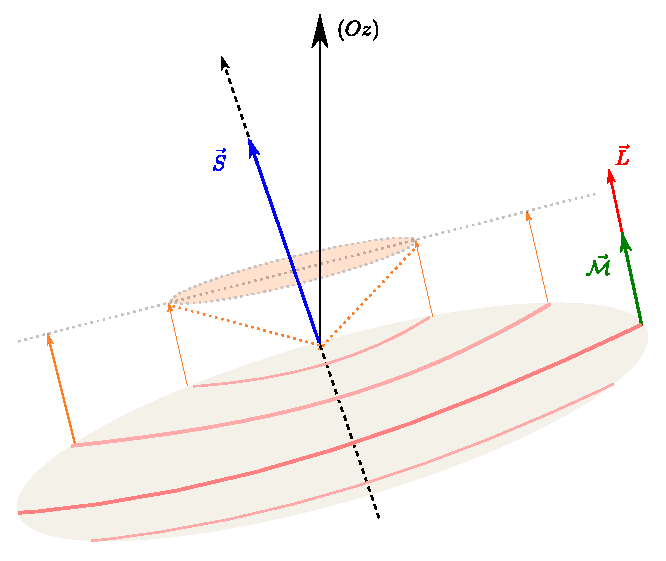
\includegraphics[width=0.8\columnwidth]{moments-cinetiques.pdf}
		\caption{\footnotesize{\textbf{Angular momenta of the blades.} The blade (in light brown) makes an angle with the vertical (represented by the $(Oz)$ axis), a mark of electric charge. The orbital angular momentum $\vec{L}$ is perpendicular to the blade, while the magnetic angular momentum, assimilated to the magnetic moment, in green, is collinear to it. In orange, the flux at a given location therefore depends on the radius. Spin is the magnetic flux density -- the Poynting vector -- thus the average of the flux over the blade's surface. The flux, as well as the spin, is perpendicular to the surface. The figure is not to scale.}}
	\end{figure}
	
	One must remember that the blade is a helicoid blade and that it is better represented as follows (up to variable thickness):
	\begin{center}
		\begin{tikzpicture}
			\def\a{0.2}
			\def\b{0.25}
			\begin{axis}[
				view={120}{30},     % View angle
				width=\columnwidth, height=\columnwidth,
				axis lines=none,    % Hide axes
				xmin=-8, xmax=2,
				ymin=-7, ymax=5,
				zmin=-1, zmax=4,
				colormap/viridis,
				]
				\addplot3 [
				mesh,               % wireframe
				shader=interp,      
				opacity=0.9,        
				domain=0:4*pi,      
				domain y=0:2.5,     
				samples=100,         
				samples y=20,
				] (
				{(1 + (1/7)*x)*y*cos(deg(x))},    
				{(1 + (1/7)*x)*y*sin(deg(x))},    
				{\b*x}
				);
				\draw[thin, -stealth] (axis cs:0,0,0) -- (axis cs:0,0,4) node[right] {$(0z)$};
			\end{axis}
		\end{tikzpicture}
	\end{center}
	
	\MQ\ has chosen to consider the set $\vec{S}+\vec{L}$ as characteristic of the quantum object. In reality, spin is not totally independent of the intrinsic magnetic angular momentum, as it is the sum of it over 2 turns.
	
	Indeed, if we consider the node from an energetic point of view, thus of work, we have
	\begin{equation*}
		\left\{
		\begin{split}
			\delta W &= P(t) dt = S dt \\
			\delta W &= \mathcal{M} d\theta
		\end{split}
		\right.
	\end{equation*}
	or
	\begin{equation*}
		S = \mathcal{M} \frac{d\theta}{dt} = \mathcal{M} \omega
	\end{equation*}
	
	As the rotation speed of the vorespace is half that of the neutrino, we obtain for any massive particle:
	\begin{equation*}
		S = 2  \mathcal{M} \omega = 2 \frac{q_e}{2 m} = g \frac{q_e}{2 m}
	\end{equation*}
	
	The \textit{Lande factor}, emerged somewhat miraculously from the Dirac equations \cite{dirac1928quantum}, is in reality only the expression of the mass (and thus magnetism) of the particles being measured, i.e., massive particles.
	
	However, the measurement of the Lande factor shows that it is not rigorously equal to 2, but to 2 "plus one \R{2}{1000}." The neutrino thus rotates slightly faster than twice the speed of the vorespace. If the factor were exactly 2, it would be a fractal factor that would not change the properties of the vorespace, namely that the photon "passes through" the vorespace. But since the factor is very slightly larger, the geometry of the blade is very slightly modified, and the photon can no longer "pass through" the massive node: it will strike it, transferring its momentum, creating the electromagnetic interaction.
	
	Note that we could have directly intuited this result by simply saying that the vorespace flux is half that of the neutrino.
	
	Note finally that by choosing the projection of $\vec{L}$ as the magnetic quantum number, \MQ\ creates a confusion of genres. Certainly, orbital angular momentum is related to magnetism, in the sense that the latter is induced by rotation, but it would have been much more fortunate to name the quantum numbers $m_l$ as the projections of $\vec{\mathcal{M}}$. It may be very difficult to restore order due to habit. But the ease of understanding the underlying domains would have gained enormously...
	\medskip
	
	We can now link the Lande factor with the fine-structure constant. Consistent with \MQ\ calculations, the Lande factor corresponds to the enlargement of the magnetic circle. It is therefore the part of the excess radius, and we thus classically find that it is proportional to the fine-structure constant and that its proportion factor is the turn of a complete circle:
	\begin{equation*}
		g = \frac{\alpha}{2\pi}
	\end{equation*} 
	
	Mass, or magnetism, therefore induces a more subtle transformation than a simple widening of the blade surface and its thickness: it induces a swelling of the thickness that rounds off, somewhat on the model of an inner tube. This elongation, relative to the thickness, is exactly the Lande factor, roughly \R{2}{1000}.
	
	This surplus makes the passage of the photon impossible. Where it once passed by brushing against the vorespace, the extra thickness of the massive nodes blocks it, mechanically inducing an interaction between photons and $S_3$-type nodes.
	
	Furthermore, the blade radius being proportional to the node size, we find the logarithmic law of the fine-structure constant \eqref{eq:structure-fine}.
	
	Finally, the apparent speed of the neutrino, double that of the vorespace, should not hide that only the magnetic blade carries the real speed, i.e., triple that of the vorespace. The excess speed consequently applies only to this blade, which therefore rotates slightly faster than 3. For the electron, it rotates at $3.002\,319\,304$, or slightly more than 7\,\% over the theoretical speed. We find the jump of slightly more than \R{7}{100} stated in the fractal law.
	\medskip
	
	Unfortunately, I have not been able to calculate the exact value of $g$ (or $\alpha$). Either this requires a more astute mind, or this constant is intrinsic to the plenum, and is therefore the only true fine constant of the universe. The Big Bang model proposed below may lean in favor of this hypothesis: it would be the exact setting corresponding to the amount of energy necessary for the creation of the neutrino which allows for the development of the electromagnetic interaction in the universe.\footnote{The fact that this is the only rigorously undemonstrable "anomaly" bothers the author. All \PQ\ is structurally mechanical and explainable, and this should also be the case here. If it is true that it is impossible to calculate this constant, then it would indeed be the only fine-tuning of the universe.}
	
	\subsubsection{Other constants of physics}
	
	One should take the time to reconstruct all the constants of physics, even if, at this stage, one can very well reconstruct everything mechanically with those already found, as this is \textit{grosso modo} what current physics does.
	
	It should be noted that one constant has no real meaning: the Planck charge. It is a simple side effect of extrapolating Planck units to all characteristics of physics: by postulating a Planck charge and defining it as the elementary charge carried by a Planck particle—a particle of Planck size. We thus have a physical impossibility of representing such a particle, unless it is associated with two vorespaces or two neutrinos. The previous definition refers to the Schwarzschild radius, i.e., to the maximum mass of an object; therefore, it would rather be an assembly of neutrinos. However, by definition, neutrinos have no charge!
	
	\section{Equivalence of Quantum Plenodynamics with current physics}
	
	\subsection{Introduction} 
	
	It is necessary to ensure that \PQ\ is compatible with all of physics if it is to claim to be a physics of everything. It was built on mechanics and thermodynamics, as well as on electromagnetism. It is already compatible with these theories. However, it must still pass the test of the three great theories of physics: special and general relativity, and quantum mechanics.
	
	\subsection{Special Relativity}
	
	Regarding special relativity, this is the easiest part, because \PQ\ was built precisely by respecting the foundations of special relativity, namely a transfer of information based on the speed of light as the maximum speed.
	
	In a way, \PQ\ can be seen as the real counterpart of special relativity, which usually happens to be a general framework, valid everywhere. \PQ\ therefore embodies special relativity.
	
	It is easy to find the Lorentz factor in a moving particle. Its "caterpillar-like" evolution marks a difference between the start of its displacement and the end, which can be triangularized in a right-angled triangle, allowing the extraction of the Lorentz factor.
	
	Time does not dilate strictly speaking, but the re-attachment time of the caterpillar lengthens, as the path to be traveled becomes increasingly large.
	
	Similarly, the tension in the caterpillar increases with speed, which in return results in an increase in mass, proportional to this tension.
	
	\PQ\ is therefore fully compatible with special relativity: one can even say that \PQ\ \textbf{is} special relativity.
	
	\subsection{General Relativity}
	
	Part of the work has also already been carried out within the framework of general relativity. Thus, in Einstein's theory, a mass curves spacetime; in \PQ, a mass acts on the plenum by imprinting a shear wave upon it, the mass phonon.
	
	Where Einstein shows that light follows a geodesic of spacetime, the photon of the plenum follows the mass phonon as an entropic surfer. It moves up the entropy thalwegs, which lead toward the masses.
	
	In Einstein's spacetime, near a mass, time slows down. In the plenum, the mass phonon decreases the entropic transfer capacities, penalizing the transfer time: the more massive the phonon, the more the transfer time is penalized. Mass indeed acts as a time retarder around itself.
	
	Finally, general relativity postulates the equivalence between inertial mass and gravitational mass. In \PQ, gravitational mass is the mass of the vorespace, the tension that can be applied to a turbine. Inertial mass is that generated by the inertia of this vorespace. By construction, they are identical.
	
	\PQ\ is therefore fully compatible with general relativity.
	
	\subsection{Quantum Mechanics}
	
	\subsubsection{Introduction}
	
	We now enter the final stage. If we can prove the equivalence between \PQ\ and quantum mechanics, we will then have united the three great physics, and \PQ\ will definitively be compatible with a physics of everything.
	
	We will conclude this part with the construction of the atomic model according to the point of view of \PQ—a model that will allow not only for the modeling of the atom but also for explaining why it functions this way.
	
	\subsubsection{Wave-particle duality}
	
	It goes without saying that the phonon of mass and charge (if needed) around a particle constitutes the famous wave of quantum particles. It is no longer mysterious at all, since it is simply the interaction of a mass—a corpuscle, then—with the plenum.
	
	
	
	This wave nevertheless has interesting properties. It is a composite heptagonal standing wave, in the sense that it is simultaneously the sum of the waves of each of the particle's sub-nodes and the rotation of the particle itself.
	
	Thus, in the case of the electron for example, composed of $2^{24}$ neutrinos, it is the composition of $2^{24}$ heptagonal mini-waves mixed with a heptagonal wave of the electron itself. \textit{Technically, the wave is therefore not composed of an infinite number of waves, but of a finite number.} Of course, the composition makes this number "large enough," which makes the "infinite" approximation acceptable as a first step.
	
	Note that the wave entirely defines the position of the particle. One could study only the wave and account for the characteristics of the particle. From this point of view, the wave indeed "pilots" the particle, which was Louis de Broglie's point of view.\cite{debroglie1924recherches}
	
	However, it is indeed the particle that gives rise to the wave, and it is more accurate to say that \textit{the particle pilots the wave}. It is therefore not \textit{stricto sensu} a pilot-wave, but rather a \textbf{pilot-particle}, if we want to keep Louis de Broglie's terminology.
	
	Note a major difference between the two theories: determinism is absolute in \PQ. It "suffices" to calculate what the wave looks like to determine what the particle looks like, and vice versa: since one and the other are in a relationship of total equivalence—in bijection, mathematicians would say—knowing one is enough to know everything about the other.
	
	This equivalence answers the great quantum question of what exactly the wave function represents. The Copenhagen school asserts that it contains the seeds of everything that can be known about the properties of the quantum particle. This is correct, in the sense that it is generated by the quantum particle in question, according to a deterministic relationship that takes into account all its states. Quantum mechanics takes this wave function as the reference for information, whereas the real reference is the particle. In a way, quantum mechanics follows an object lit by the sun by following its shadow. When quantum mechanics measures the shadow, it then turns its gaze toward the object and claims that the shadow has transformed—collapsed—into the object. In reality, \textit{quantum measurement is just a change of point of view.}
	
	Finally, we saw earlier that wave-particle duality and the quantization of momentum mechanically led to de Broglie's formula.
	
	\subsubsection{The case of the photon}
	
	The photon, our entropic surfer, poses a real problem. By construction, it is only a wave. Duality does not apply to its case, which is bothersome, to say the least, for Albert Einstein, who received his Nobel Prize after explaining the threshold of the photoelectric effect by the presence of light corpuscles!
	
	Indeed, \PQ\ fully assumes changing the status of the photon in physics. Just as it explained the real nature and the origin of the photon, it assumes that the photon is only a pure wave.
	
	The question that then immediately arises is: how to explain that thousands of physics experiments over recent years highlight the dual nature of the photon? The answer is contained in the question: it is not the nature of the photon that the experiments measure, but... the instruments themselves. Thus, when a photon approaches a physical detector, the latter, by its atomic composition, influences the plenum by creating a mass phonon, and sometimes even a charge phonon. The photon, as a phonic surfer, immediately "obeys" the change in the plenum, creating the illusion that it too is endowed with a dual nature.
	
	This is perhaps the biggest revolution brought by \PQ: physicists have actually been measuring their instruments for years when they implement photons!
	
	\subsubsection{The role of measurement}
	
	This is a perfect transition to examine the role of measurement. Independently of the particular case of the photon, which is nonetheless the privileged actor of current experimental physics, one must look at the notion of measurement in general.
	
	In \MQ, measurement impacts the state of the system, reducing it to an eigenstate—the one measured. \MQ\ postulates that some state out of all the superimposed states was drawn by lot, according to true chance. The system is then irremediably reduced to the measured state.
	
	We saw above that, in reality, quantum measurement is a change of point of view. There is no collapse of the wave function, for the good reason that nature reveals the real, and the real is the object, not its relationship with the ether, even if this relationship can indirectly define it. It goes without saying that when physicists measure an electron, it is indeed the \node{$S_3(-1,1)$} object they expect to see and measure, not the heptagonal wave surrounding it, even if the latter is not without consequence for the measurement.
	
	We have indeed seen that measurement is not without impact at the level of \PQ. Indeed, measuring instruments, macroscopic by essence, have a direct impact on the plenum. \textit{They are therefore not neutral}. To truly experiment, the physicist must remove the bias introduced by the instrument itself. It will be complicated to completely free oneself from this bias when measuring quantum-sized objects.
	
	Take, for example, the classic case of electron interference through two slits. The electron possesses a wave, certainly. It can very advantageously interfere between two openings, forcing the electron's passage through one rather than the other.
	
	But what is the part of the mass phonon of each opening in this story? Around the two openings, two phonon corridors are created... Are we certain that each opening is atomically and rigorously the mirror of the other (otherwise, their mass phonon might differ and, thus, favor one measurement over another)? Furthermore, one must be certain to "hit right in the middle of the slits," because electron launching is deterministic in \PQ. That is to say, in theory, by launching the electrons identically, they should follow exactly the same trajectory and all pass through the same hole. Of course, any small thing along the trajectory is enough to change a micro-parameter and change the final result. And the surrounding air is full of interference!
	
	Of course, statistics often come to save the experiment: given the large number of uncontrollable parameters, it is reasonable to estimate that they statistically annihilate each other. One should therefore find experimental accuracy via statistics.
	
	Regardless, the question arises of what we are really measuring today in physics... at least at the quantum level when working on interference.
	
	It goes without saying that as soon as the mass or charge phonon can have an impact on any measurement, it must be taken into account, if only to gain some distance from the result.
	
	\subsubsection{Entanglement: the lure of chance}
	
	The famous EPR article\cite{einstein1935can} by Einstein, Podolsky, and Rosen launched a debate that ended recently, but which \PQ\ proposes to restart, with an unexpected conclusion. The experiment postulates that if \MQ\ is correct, then there exists a state of entanglement between two particles and that this state violates special relativity, since the information circulating between the two particles would circulate faster than the speed of light. Aspect's experiment\cite{aspect1982experimental} showed that this assertion was verified.
	
	Yet, \PQ\ asserts that determinism exists and that, in fact, entanglement does not exist. It is simply a side effect of quantum mechanics theory, which is not the simplest representation of reality, but a more complex theory, as mentioned by Poincaré\cite{poincare:1902:sh}.
	
	Quantum mechanics thus takes an indirect path to express quantum effects. The path of \PQ, being more direct, does not possess the side effects of quantum mechanics.
	
	Indeed, quantum mechanics hides what it does not know under the name of quantum chance. Not being able to calculate the real characteristics of a quantum particle, it has developed a divinatory technique—excellent, for that matter—to explain the behavior of quantum objects. But this technique postulates the idea of irreducible chance, therefore structural indeterminism, which is not a reflection of reality.
	
	Take the example of two electrons in a helium atom. They are entangled, in the sense that each has a spin opposite to the other. \MQ\ asserts that only measurement lifts this indeterminacy. In reality, there is no indeterminacy: each electron really possesses a spin opposite to the other. If you measure one, you do not change the value of the other. Entanglement is a consequence of the structure (which will be explained in the atomic model), not of measurement. Entanglement therefore does not exist from the point of view of quantum plenodynamics. You can move two entangled objects each to one end of the universe and measure one; no information will circulate to the other: both values are determined before the measurement.
	
	Thus, the EPR article, which supposed quantum mechanics was correct to postulate what followed, remains accurate: it is just that the starting hypothesis—the accuracy of \MQ—is not conformable to the real. Quantum mechanics uses a non-realistic chance that has consequences within quantum mechanics, not in reality. Entanglement exists in quantum mechanics, not in reality, because quantum mechanics does not represent the real, but a mathematical and complicated way to describe the real. This is a superb illustration of the dangers of using mathematics to describe physics, as stated by de Broglie\cite{debroglie1976physique}.
	
	So, how is it that Aspect's experiment is correct? For exactly the same reason that experiments on photons are correct: they do not measure entanglement \textit{in se}, but the interaction of photons with the instruments. To compensate for this interference from the sensors—here, waveplates—one would have to measure the photons with objects of the same nature as the photon itself. Quite a challenge!
	
	Regardless, this in no way detracts from Alain Aspect having achieved this extraordinary experiment.
	
	\subsubsection{The Pauli Exclusion Principle}
	
	The Pauli exclusion principle postulates that two fermions in the same place cannot have identical characteristics. This principle follows naturally from the $S_3$ structure of fermions which, to be together, must have compatible physical characteristics: for example, to assemble two $S_3$ nodes, one must be flipped, thus reversing its spin, so that the screwing directions are compatible. This principle is therefore structural in \PQ.
	
	We will see in the atomic model a finer reason for this principle, which actually results from the minimization of the energy of electrons in atomic orbits.
	
	\subsubsection{CPT Theorem}
	
	CPT conservation is structurally maintained in an $S_3$ node by the symmetry of the first 64 states and the following 64. Reversing chirality requires passing through all intermediate states. CPT symmetry is ensured by the turbine's structure.
	
	Regardless of the nodes, the 128-state structure is structurally compatible with CPT conservation.
	
	\subsubsection{The Heisenberg Uncertainty Principle}
	
	\PQ\ does not challenge the Heisenberg uncertainty principle. Indeed, the latter does not depend on the mathematical theory of quantum mechanics: it is an "obvious" observation that two linked characteristics cannot be measured at the same time, as the respective measurement times are not compatible with each other.
	
	Furthermore, the spatio-temporal quantization of the plenum makes the uncertainty principle trivial.
	
	\subsubsection{Conclusion on compatibility}
	
	\PQ\ and \MQ\ are therefore fully compatible. \PQ\ simply allows for a slight correction of \MQ, whose intrinsic chance led to conclusions that were sometimes... hazardous. Determinism regains its full rights in the quantum world, which is no longer bizarre, as quantum particles have regained a determined trajectory.
	
	\subsection{The atomic model}
	
	\subsubsection{Introduction}
	
	Until today, physics has observed that the atom exists and has deduced a model based on purely experimental data. It is a classic case of a "law" extrapolated from experimental observations\cite{poincare:1902:sh}. While the model is correct because it fits the experiment, it offers no explanation for "why" things function this way; in particular, it provides no answer to the \textbf{big question}: "why doesn't the electron fall into the nucleus?", a question that could be posed via its contrapositive version: "why does the electron orbit without spending energy?" \PQ\ proposes to resolve this enigma and to provide, for the first time, a consistent answer.
	
	Without going into details, the general idea of atomic construction is to find a natural stable state from elementary particles. The latter are only a step before the final stabilization, which is the atom. Stabilization in the plenum is always ensured by a node self-similar to $S_3$; thus, unsurprisingly, we will find this structure in the atom. The electron and the nucleus will play the role of the blades and "tangle" to form an $S_3$-type node. Of course, at this advanced stage of the particles, fusion will no longer be physically possible, and the $S_3$ node will be strongly distended: the electron and the nucleus will therefore no longer be stuck together.
	
	On the other hand, this spacing leaves free room to form a complex entanglement of $S_3$ nodes, where each added node will correspond to an atom in Mendeleev's table. Nature so much needs to embrace this $S_3$ node shape to stabilize itself that the entire set of electron shells itself forms an $S_3$-type node!
	
	So, ready for the journey to the heart of the atom? Let's go...
	
	\subsubsection{Foundations of the atomic nucleus}
	
	We saw that quarks, to converge toward a stable $S_3$-type node structure, associated in triplets to form a neutron and a proton.
	
	Technically, nature could have stopped there, but the presence of electrons will force neutrons and protons to find a common node shape for even more stability.
	
	One might be surprised to include the neutron in the problem, as a simple proton-electron association is enough, for example, to ensure electrical neutrality. But this association alone does not allow the entire set of possible nodes to unfold—only to initiate it. The neutron will provide the "glue" allowing for the construction of this set. For now, let us admit the necessity of including the neutron to build the nucleus and study what happens.
	
	The only stable form for a proton and a neutron is to form an $S_3$-type node, thus a winding of three quarks. This is a slightly hybrid model compared to the standard plenum model which requires only a double helix. Here, we have a triple helix, and it is reasonable to admit that the double helix composed of the same quarks plays a unique role, that of the second helix in the standard model (of \PQ!). Indeed, if there are three helices, the resulting object is no longer a spinor. A doubt persists as to which of the two helices will work in concert with the other. It is more "Ockhamian" to choose identical quarks to play a similar role.
	
	The proton and the neutron are therefore technically $S_3$ nodes—that is, turbines, like the vorespaces of the plenum. To associate, they must therefore follow the rules of turbines, and thus allow the interlocking of the screw threads. A neutron and a proton must therefore present themselves head-to-tail, in order to rotate in opposite directions, so as not to repel each other. The general appearance forms a torus. The spin of the whole is 0.
	
	Note that in nature, this is a poorly stable node, hence the need to unite with a third party to form a more stable node. We will stop there for now to build our first model of the atom, as the structure of the nucleus itself will later deserve a dedicated section.
	
	\subsubsection{Foundations of the atomic model}
	
	Let us take the example of the hydrogen atom to begin with: its apparent simplicity will powerfully help us understand what follows. Until today, physics considers the hydrogen atom as being composed of a positive charge, the proton, and a negative charge, the electron. This is correct, but only in appearance.
	
	In reality, the proton is not the opposite charge of the electron: we have seen that the opposite is the positron, which is an \node{$S_3(1,1)$}. The proton, for its part, possesses the \textbf{apparent charge} of the positron, but its distribution is totally different: it is composed of two \Ru{+}{2}{3}{e} charges and one \Ru{-}{1}{3}{e} charge. If one were to compare the "protonic turbine" to the "positronic turbine," they would not look alike at all. The latter is an inverted electron turbine—therefore, an upside-down conical screw rotating in the opposite direction of the electron—whereas the proton likely resembles a screw with two throats: a wide one well below its midpoint and a smaller one just above it. Most importantly, there is a massive difference:
	
	\textit{The two helices of the proton rotate simultaneously.}
	
	It follows that the classical model of the hydrogen atom based on a pure negative electric charge and a pure positive electric charge is false. The positive charge is composite: it emits two charge phonons corresponding to the \Ru{+}{2}{3}{e} charge and one charge phonon corresponding to the \Ru{-}{1}{3}{e} charge. If the \Ru{+}{2}{3}{e} helices work in concert, we can reduce the first two phonons to a single double phonon of \Ru{+}{4}{3}{e}.
	
	Since the helices are entangled, the phonons are as well. There is therefore interference, and a phonic field is created around the nucleus—a composition of the previous heptagonal waves, with peaks at \Ru{+}{4}{3}{e}, peaks at \Ru{-}{1}{3}{e}, and peaks at $e$. Of course, all combinations exist. Globally, pseudo-circular zones will exist around the proton in which one charge will be privileged.
	
	When the electron arrives in such a field, it is guided by the thermodynamics of the plenum. It follows the paths of low energy, i.e., the valleys of negentropy. Its negative charge does not change: it is a true $-e$ charge. It will therefore follow an equilibrium path between the \Ru{+}{4}{3}{e} thalwegs and the \Ru{-}{1}{3}{e} thalwegs. This is a low-energy path that consumes none: the electron orbits effortlessly.
	
	However, it passes in front of charge peaks and is forced to adapt to each of them: \textit{it must therefore flip itself over to present a charge opposition that naturally maintains it in the low-energy valley}. The electron oscillates, and its spin alternates each time it presents itself before a new charge, the charges being distributed uniformly around the trajectory. The electron thus oscillates regularly throughout its satellite trajectory.
	
	
	
	We can once again pay tribute to the vision of de Broglie, who proposed a very similar model of electron oscillation during its trajectory, giving it a specific wavelength.\cite{debroglie1956tentative} In reality, once again, the model must be inverted: it is the trajectory that imposes the oscillation; the electron does not oscillate on its own, at least not in this case.
	
	What happens when a neutron is added? The hydrogen atom becomes deuterium, and the neutron espouses the proton according to the process mentioned previously. Once again, current physics "sees" a zero charge in the neutron, but if that were the case, it would be an \node{$S_3(0,1)$} node—a pure mass, i.e., a neutrino. The neutron is composed of two negative \Ru{-}{1}{3}{e} charges and one positive \Ru{+}{2}{3}{e} charge. By a reasoning analogous to the previous one, a "gagged" double helix is formed, where both work in concert, those of the same charge being synchronized. To the previous field must be added a new one, which is the superposition of the two aforementioned phonons. Fortunately, this is a near-field that changes the existing field very little. It merely "tightens" the trajectory very slightly.
	
	We can measure this difference through ionization energies by adding tritium, with one more neutron:
	
    \end{multicols}
	\begin{center}
		\begin{longtblr}[
			caption={\footnotesize{\textbf{First ionization energy of the first three atoms}}},
			label = {tblr:5-0-4},
			]{
				colspec={Q[c,m]  Q[c,m] Q[c,m] Q[c,m] },
				rowspec={Q[c,m]},
				row{odd}={bg=blue!10!white},
				row{1}={c,mode=text,fg=white,bg=pkcolor, cmd=\textbf},
				rowsep=2pt, colsep=3pt,
				vline{2-Y} = {1}{0.3pt,gray!50},
				vline{2-Y} = {2-Z}{0.3pt,gray!30},
				hline{Z} = {0.1pt,blue},
				rowhead = 1, 
			}
			
			Isotope               & Composition                  & Ionization Energy & Difference/Protons only  \\
			Hydrogen (\ce{^1H}) H & 1 proton                     & 13.59844 eV       & --                       \\
			Deuterium (\ce{^2H}) D& 1 proton + 1 neutron         & 13.60215 eV       & $+0.00371\,eV$           \\
			Tritium   (\ce{^3H}) T& 1 proton + 2 neutrons        & 13.60338 eV       & $+0.00494\,eV$           \\
		\end{longtblr}
	\end{center}

	\begin{multicols}{2}
	This is a confirmation. The trajectory generally does not change and undergoes a slight corrective effect with each addition of a neutron.
	\medskip
	
	What happens now when a proton is added? The atom becomes helium with two protons and one neutron. We will see in the next section how the nucleus arranges itself to validate this association. At this stage, we only admit that the neutron separates the two protons so as to isolate them from each other, avoiding their repulsion as much as possible. The double interlocking of proton + inverted neutron + proton is mechanically stable.
	
	From the point of view of electric charge, a second protonic field is added to the deuterium field. As these are harmonic fields, the consequences are not catastrophic: a field similar to the previous one is built, shifted in one direction or another. Atomic radius measurements show that this field actually shifts toward the nucleus.
	
	For the desired electrical equilibrium, a second electron must be added. For the same reasons as before, the electron follows the same trajectory as the first and thus orbits in the same place.
	
	The presence of a first electron is, however, disruptive for two reasons:
	\begin{itemize}
		\item The first is that it has the same charge, so the two electrons repel each other;
		\item The second is that the first created a phonic wave, and the second will enter it.
	\end{itemize}
	
	Let us study the first consequence. The second electron will seek a location that minimizes the energy between the two due to electrical repulsion. \textit{The two electrons will therefore naturally try to place themselves at the antipodes of each other.}
	
	The second consequence is even more impactful. The phonic wave—the "de Broglie wave"—created by the passage of the first electron is an oscillating wave that propagates throughout the trajectory. The second electron, even placed at the antipodes, has two choices: fight against this wave or surf on it. Since it naturally follows the trajectory of least energetic effort, it will place itself in phase opposition. The two electrons will alternate in an opposite manner: \textit{this is the topological explanation of the Pauli rule.} Note that this is only valid because the electrons follow the same trajectory.
	
	We will stop the model there for now and return to see what is happening in the nucleus.
	
	\subsubsection{The fine model of the atomic nucleus}
	
	While we know that neutrons and protons are added to the nucleus, we do not know how they are physically structured. The model that dominates today is the shell model of the nucleus, which limits itself to structuring the nucleus into shells on the model of electrons, without explaining the physical relationships between the objects.
	
	The problem to be solved is knowing how to distribute neutrons and protons according to atomic order. Of course, the first idea that comes to mind—and it is a good one—is to separate the protons with neutrons to ensure electrical isolation and prevent a breakup due to repulsion. This is the basic rule:
	
	\begin{mybox}[breakable,colback=blue!10, colbacktitle=pkcolor]{Postulate 13}
		Every pair of protons in the atomic nucleus must be connected by a neutron.
	\end{mybox}
	\medskip
	
	Furthermore, by "screwing" a proton into an inverted neutron, one can "screw" again, adding the same pair each time.
	
	One can try many association possibilities, but nothing quickly resembles the periodic table model. One must return to the root of stability in the plenum and think that the arrangement will mimic an $S_3$ node—a growing spiral. But inter-proton repulsion will force the "tinkering" of the spiral during formation to add additional "insulating" neutrons to stabilize the structure due to the protonic overlaps that appear.
	
	To properly understand the 3D model, it suffices to project it in 2D. Everything is summarized in figure \ref{fig:6-0}.
	
	The idea is to associate a neutron with the previous proton by shifting it by $2\pi/7$ to gradually form a logarithmic spiral specific to the geometry of the plenum. Hydrogen initiates the chain, and it is deuterium that truly engages the spiral by shifting its neutron. Then, helium is formed by the addition of a proton. The overlap of the protons is sufficiently partial and does not counter the emerging spiral.
	
	However, the next atom is impossible to construct by the simple addition of a proton. Indeed, the lithium proton would then overlap with the hydrogen proton, and the electrical repulsion would force the spiral open. It is therefore necessary to simultaneously introduce a neutron with the proton, which will not only electrically isolate the two concerned protons but also mechanically link them. The spiral is thus "screwed" and must follow the path of minimal energy.
	\vfill\strut
	
	\begin{figure}[H]
		\centering
		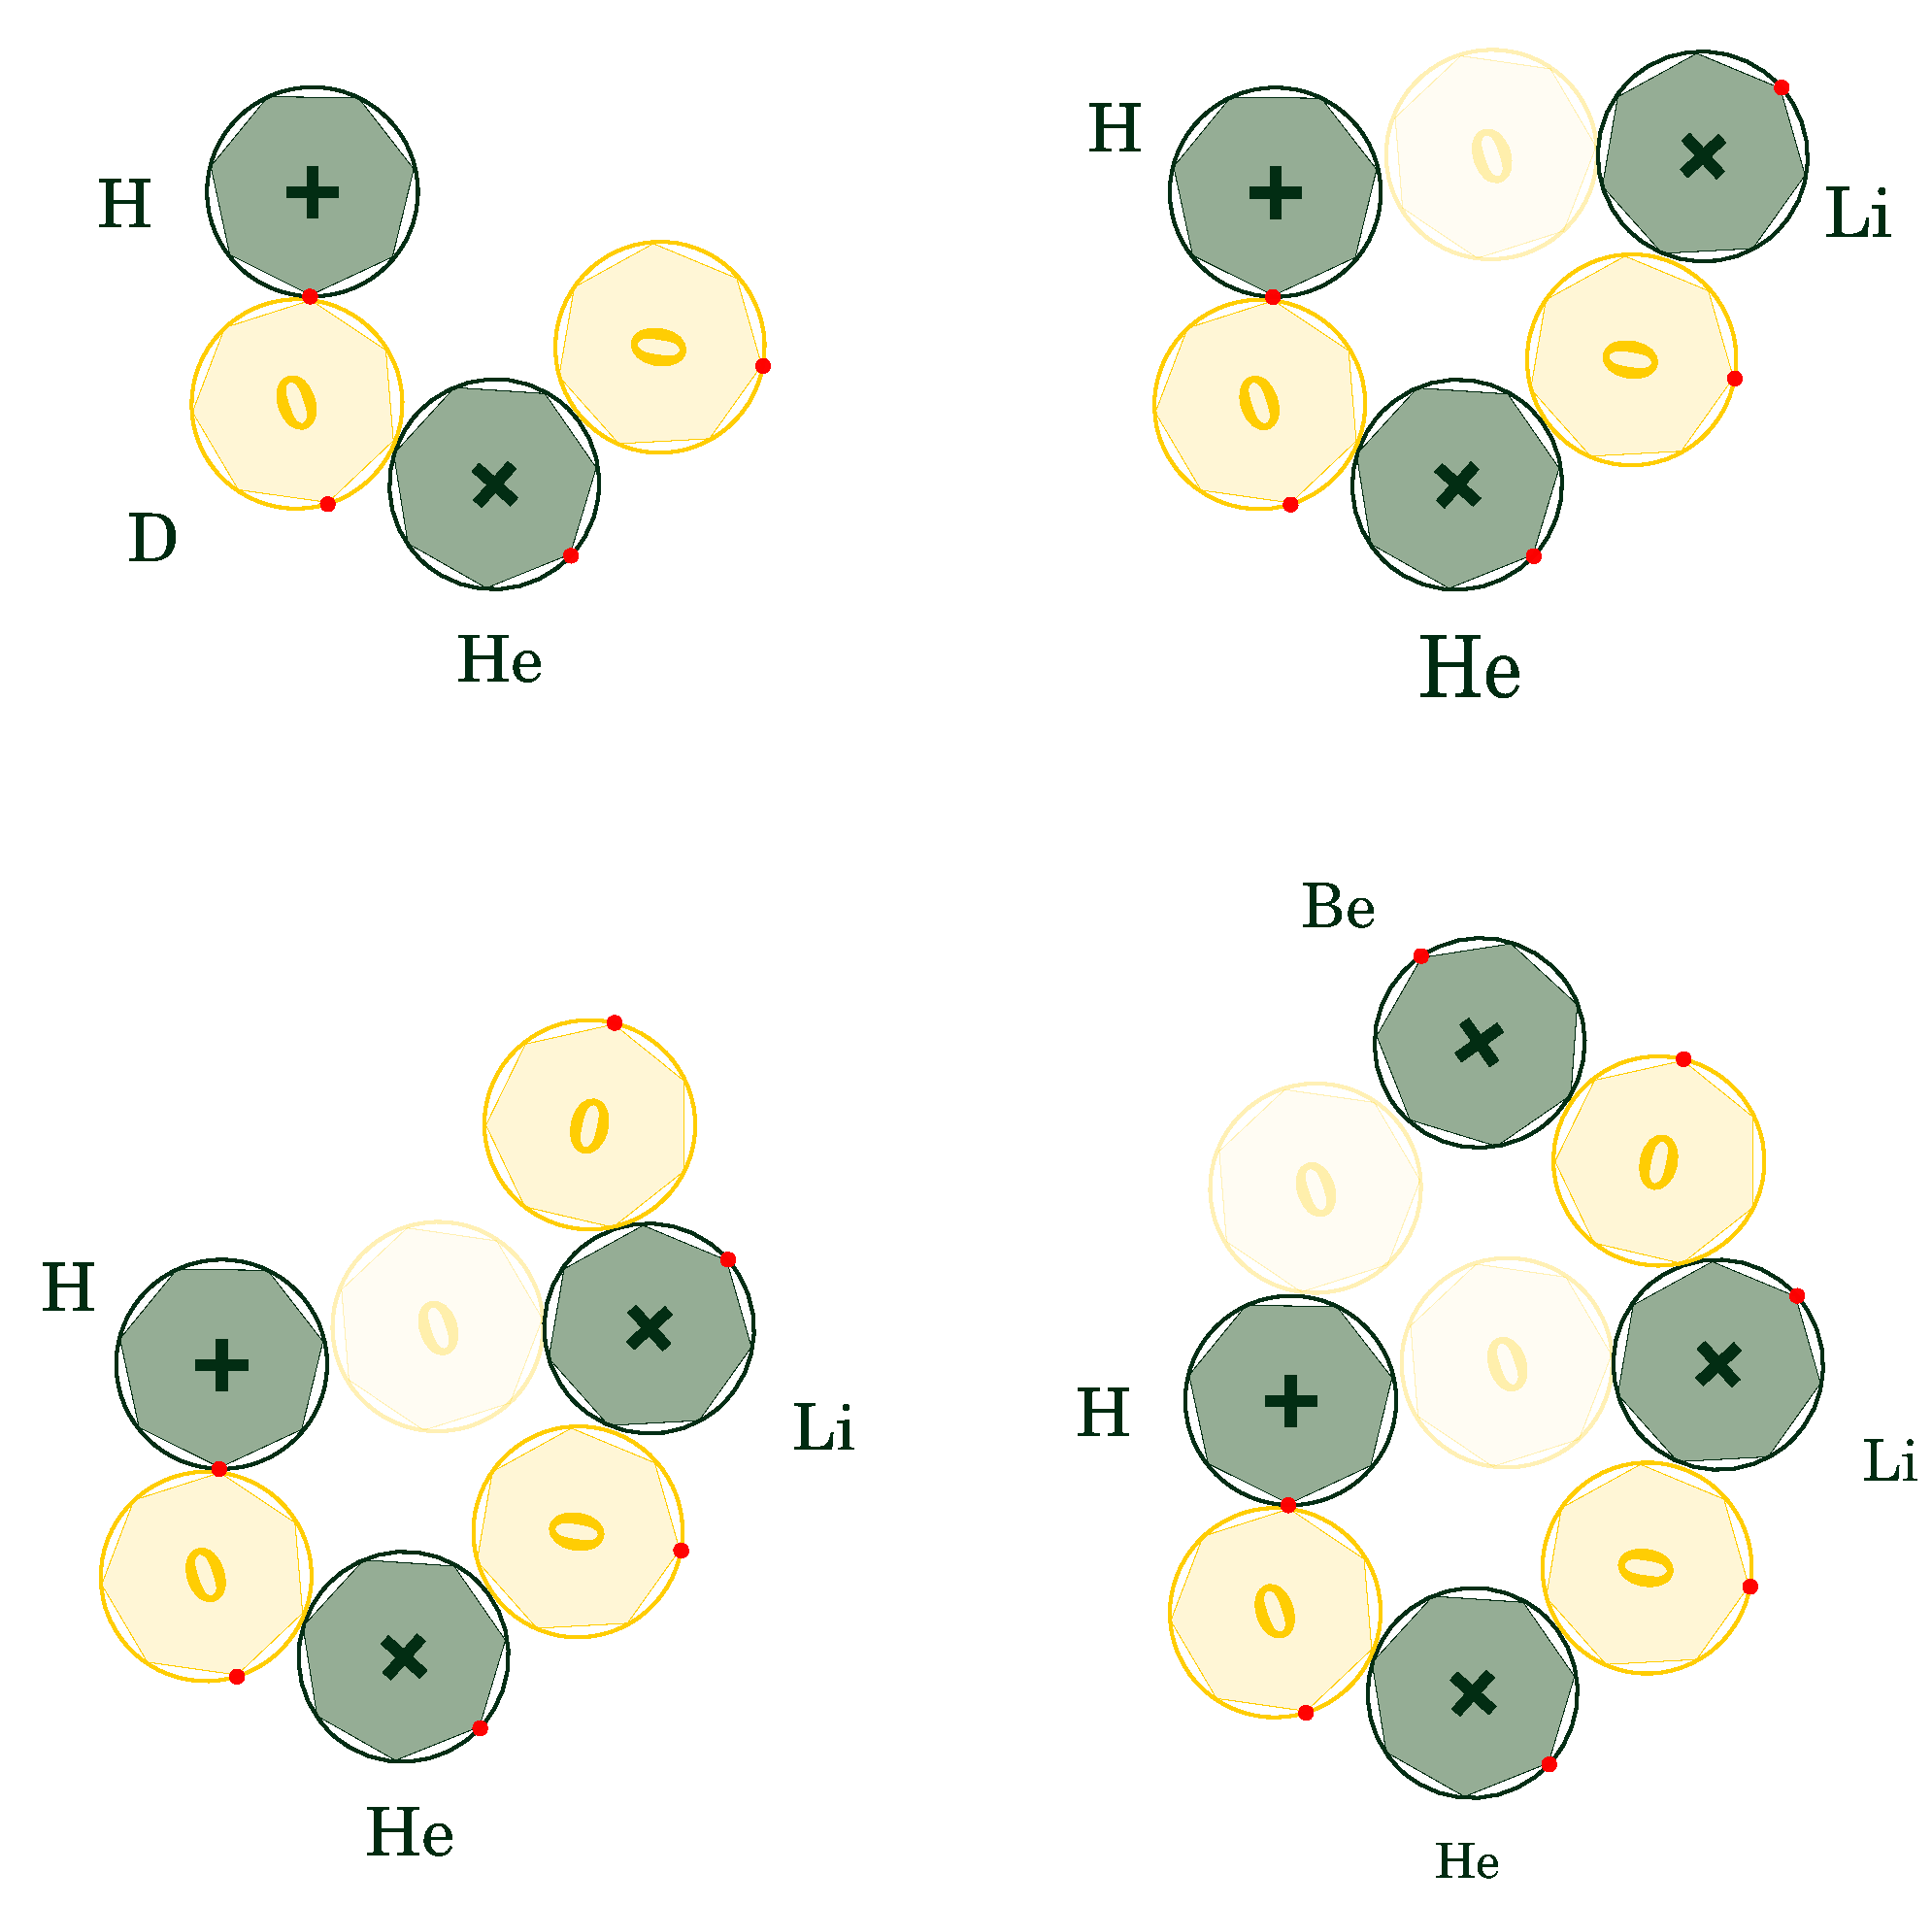
\includegraphics[width=0.8\columnwidth]{construction-noyaux-atomiques.pdf}
		\caption{\footnotesize{\textbf{Step-by-step construction of atomic nuclei.} The proton in green is linked with a neutron in yellow. The association is made by a shift of $2\pi/7$ (traceable via the red dots), creating a spiral. To prevent the spiral from bursting due to electrical repulsion, it is necessary to shift the placement of a proton (light yellow) to link two non-consecutive protons. The first neutronic link is between the lithium proton and the hydrogen proton, the second between beryllium and hydrogen.}}
		\label{fig:6-0}
	\end{figure}
	
	One can thus construct the entire periodic table. The 2D figure extended to calcium is figure \ref{fig:7-0}.
	
	Note that, although the figure was not perfectly realized (as oxygen and calcium should "meet"):
	\begin{itemize}
		\item the magic numbers \cite{goeppert1949magic} appear as completion cycles of the screw thread;
		\item we solve the jump of potassium, which requires two neutrons and breaks the series of increments of 1 in the periodic table. Indeed, it is not topologically possible to join potassium without adding a linking neutron (in blue), and it is also necessary to protect the potassium proton from the nitrogen one (in light).
	\end{itemize}
	
	The model of the nucleus is thus a spiral with 7 screw threads.
	\vfill\strut
	
	\begin{figure}[H]
		\centering
		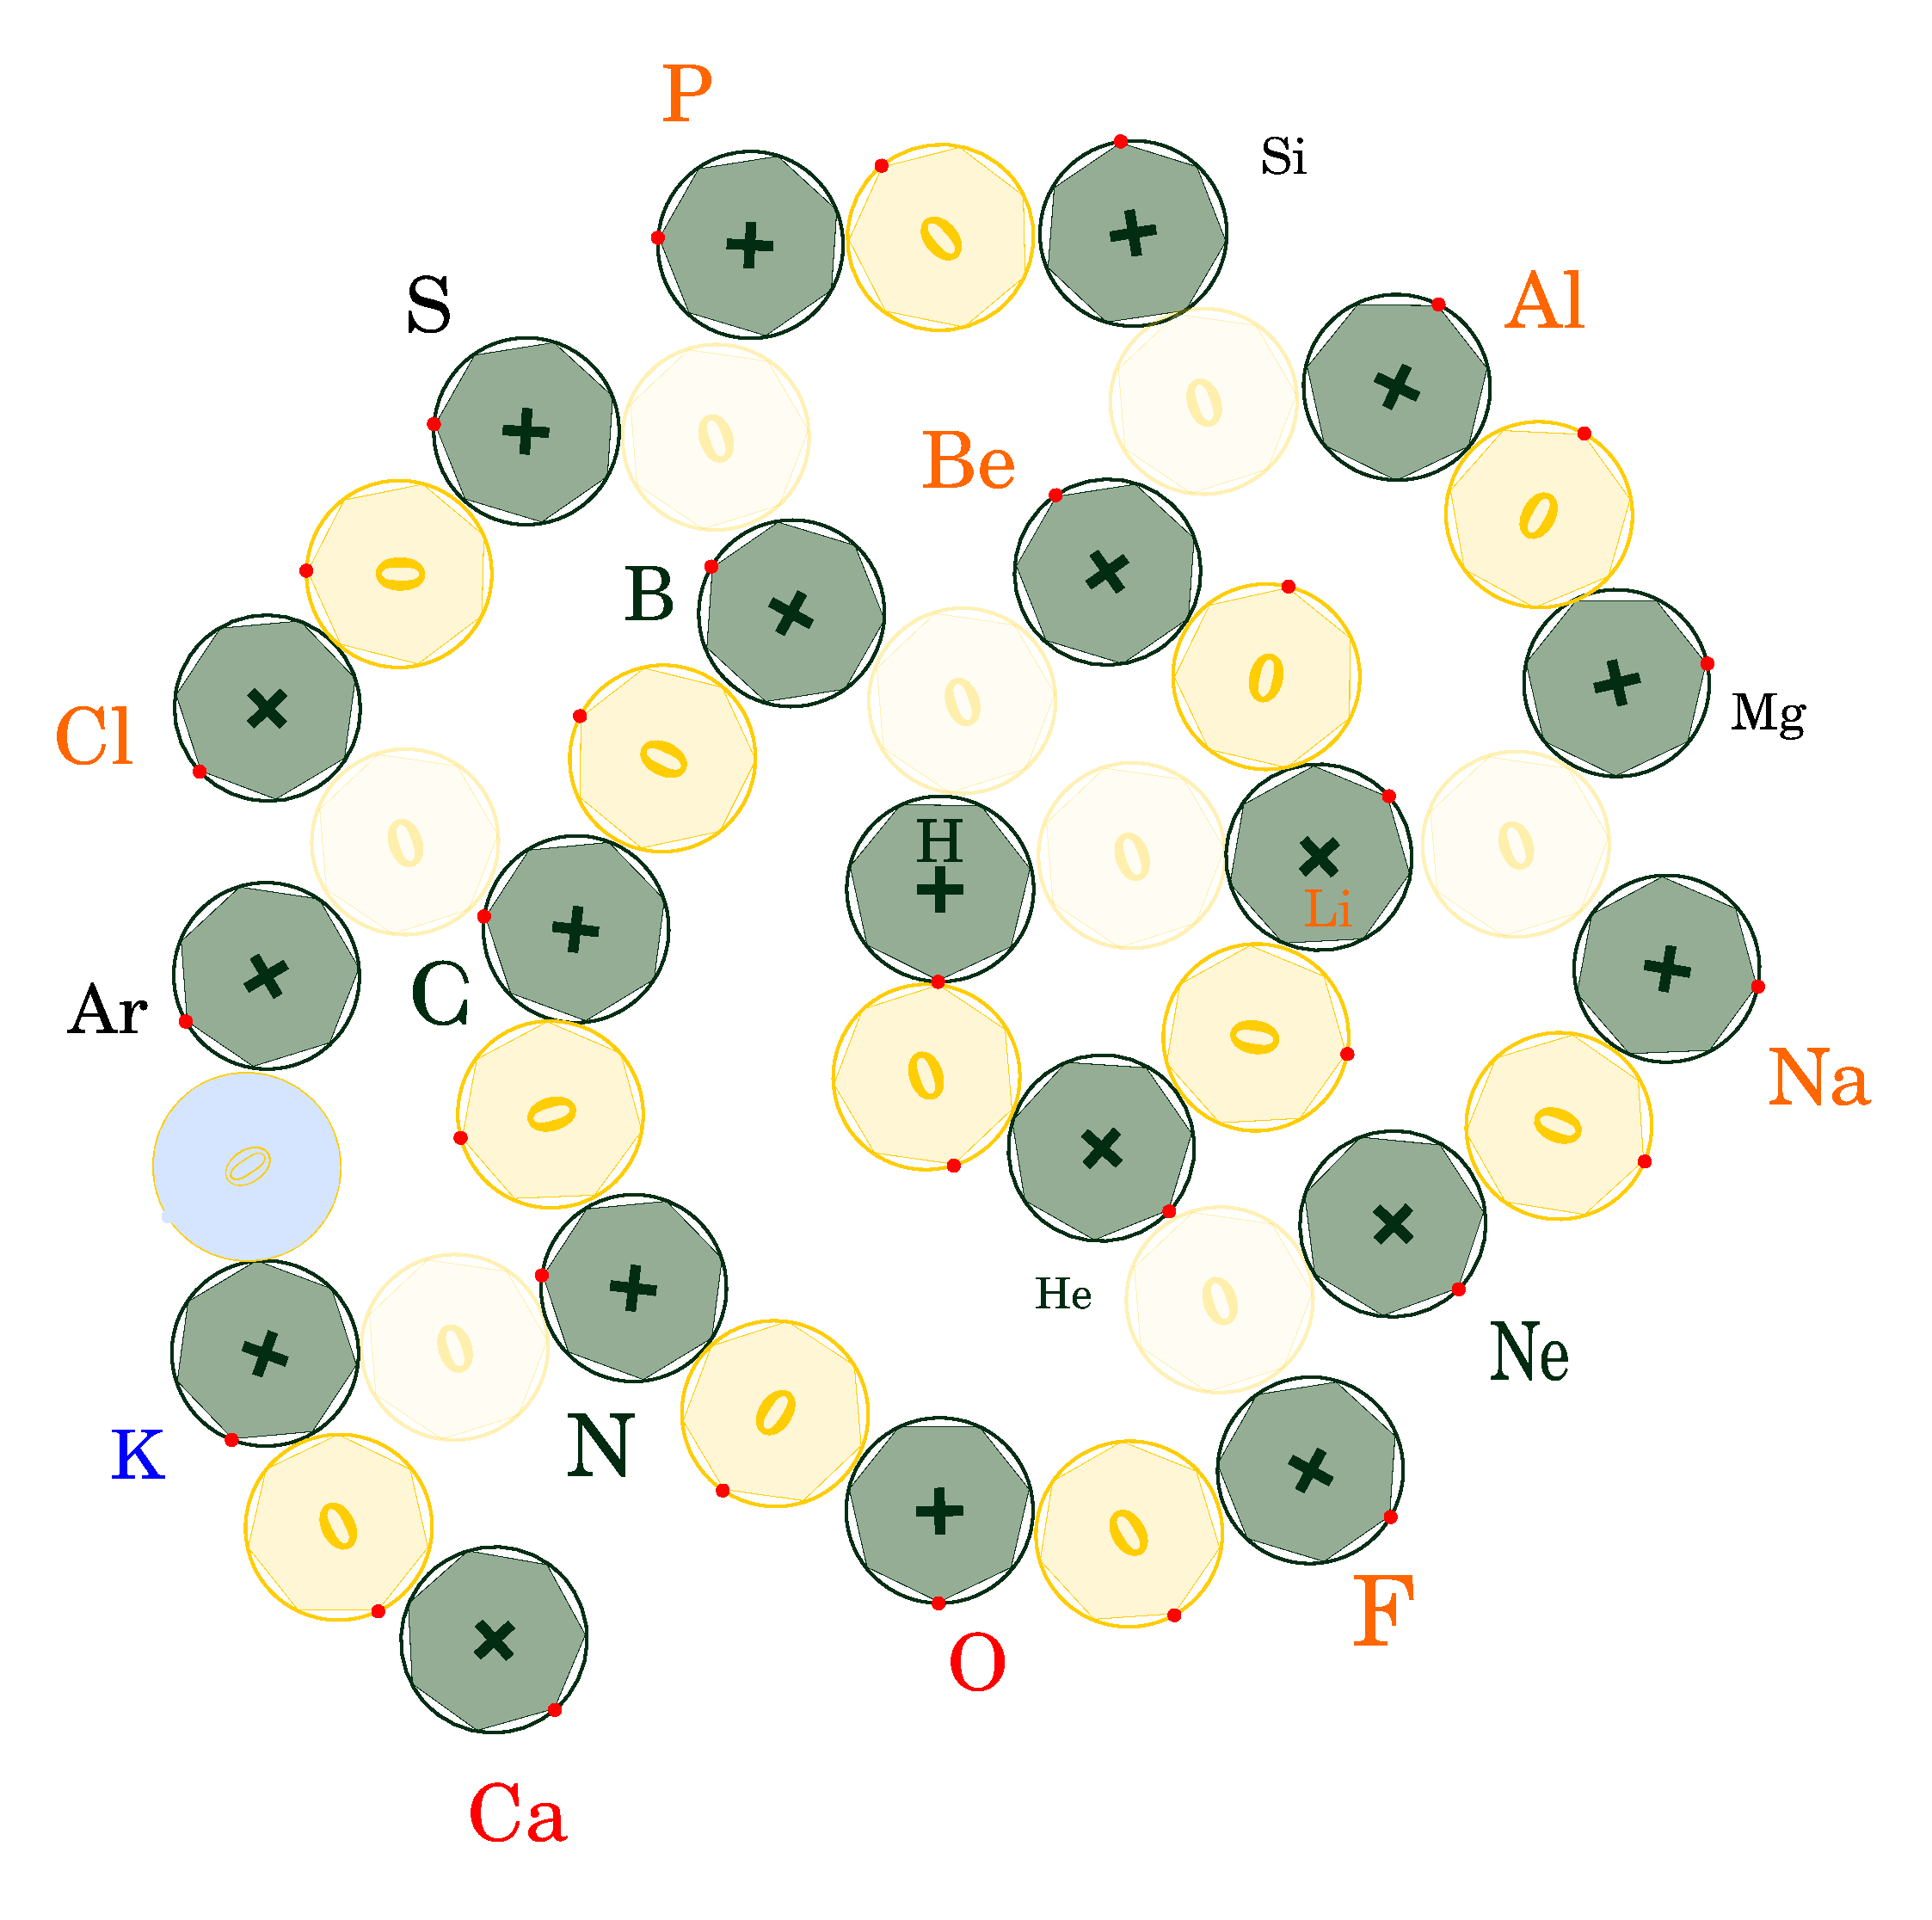
\includegraphics[width=0.8\columnwidth]{noyau-atomique-Calcium.pdf}
		\caption{\footnotesize{\textbf{2D projection of a calcium nucleus.}
				The red dots allow for tracking the rotation of the spiral ($2\pi/7$ phase shift), the light neutrons are those that must be added with a proton to balance the helix (the atom is then marked in orange). In red, the cycle ends. The projection, or more surely my imperfect spiral drawing skills, skewed the figure: oxygen and calcium should be vertically aligned.}}
		\label{fig:7-0}
	\end{figure}
	
	\subsubsection{The weak force}
	
	We have seen that the strong force is due to the interlocking structure of the $S_3$ nodes that are protons and neutrons. What about radioactivity—the weak interaction?
	
	The previous model of the nucleus allows us to imagine what happens when it enters rotation. Elements at the top of the spiral, those on the highest screw threads, mechanically have a higher rotational speed because they are on a wider disk.
	
	There exists a moment where the size of the disk, and thus the speed of the neutron-proton pairs, is sufficient to compete with the mechanical bond. One only needs to find the spot where there are few neutronic links—those that "screw" the pairs to the spiral.
	
	The pairs at the end of the helix are the ones that will tear away. The reason why they separate in doubles is not necessarily clear without calculation. It is probable that the kinetic energy of the double-pair is exactly what is needed to break a neutron-proton screw bond. It is thus a helium-4 nucleus that is ejected, causing $\alpha$ radiation.
	
	\subsection{Electronic orbits}
	
	This (too brief) overview of the atomic model must conclude with a word on atomic orbitals.
	
	The $S_3$-type model for the nucleus imposes an external field that is quite complex to calculate. While it could be relatively intuited for the first two atoms, exponential complexity makes any "hand-wavy" explanation for the following ones futile.
	
	However, at this stage, while awaiting a mathematical modeling of \PQ, we can extrapolate the results of atomic physics to introduce them into the \PQ\ model. We will therefore recover the orbitals of quantum mechanics, changing their probability perspectives to a trajectory perspective.
	
	The question that immediately arises is: why can't we put three electrons in an $s$ orbital? Simply because there is not enough room to meet all conditions simultaneously: namely, equidistance of the electrons and spin opposition by energy minimization. Introducing a third electron would force a "120° placement" of the three electrons, which would prevent an electron from being at an energy minimum. It would increase the tension of the "de Broglie wave" phonon, disrupting the balance of the system. It is simpler for this electron to place itself in another negentropy thalweg, in the orbit above.
	
	Now, let us bring the number of electronic shells closer to that of the nucleus layers. They respond to each other, obviously, because the association of electron shell and nucleus shell constitutes, in reality, a degenerate form of an $S_3$ node, the spacing between the two layers marking the degeneracy.
	
	This degeneracy is actually intrinsic to our universe, "non-finite" as we will see in the Big Bang model. It clearly indicates the final path the universe will take at its end: the undoing of all nodes...
	
	Finally, it can be added that the photon emission of the electron changing orbits finds its full utility in this model. Each orbit corresponds to a given rotation speed of the electron, hence an exergy. To change orbits, the electron must gain or lose the energy quanta necessary to increase or decrease the exergy. If the orbitals are close enough, the electron seems to jump immediately from one to the other, whereas it is actually accelerating (or decelerating) during a time that is a multiple of the number of quanta used. It would be interesting to observe the actual trajectory of the electron and the way it finds a path between the negentropy thalwegs "perpendicular" to the orbit it previously occupied.
	
	\subsection{Conclusion}
	
	\PQ\ is formally compatible with all physics, solving in the process a quantity of physical problems such as the actual functioning of the atom, the nature of the photon, or the "hoax" of quantum entanglement. It is now necessary to formalize its mathematical status to complete the theory. The next section will limit itself to giving a brief overview.
	
	In any case, at this stage, \PQ\ is a physical theory of everything.
	
	\section{Mathematical formalism of quantum plenodynamics}
	
	\subsection{Introduction}
	
	To be exhaustive, \PQ\ must also adopt a rigorous formalism. The previous qualitative approach has at least the merit of expressing in simple, concrete words and images the underlying mathematical formalism, which is much less obvious.
	
	However, and by chance, this formalism is already known and has been implemented many times to give substance to all physical theories. This is one of the reasons why it will not be developed extensively. The second reason is that the author is too weak in mathematics to do so in a reasonable timeframe.
	
	\subsection{Mathematical foundations}
	
	The space of \PQ\ is that of the Clifford algebra $Cℓ_{7,0}(\mathbb{R})$, i.e., a Euclidean space of dimension 7. It generates a series of sub-algebras of dimensions 1 to 7 which will be the foundations of the \PQ\ nodes.
	
	$Cℓ_{7,0}(\mathbb{R})$ alone is not enough to define \PQ: one must add a rotation direction, a rotation speed—the speed being the medium of energy—and a constrained dimension (norm). This quartet forms the mathematical model of \PQ.
	
	To this must be added the principle of fractality based on the sub-algebras of $Cℓ_{7,0}(\mathbb{R})$.
	
	Note that the spatial constraint does not change the algebra $Cℓ_{7,0}(\mathbb{R})$ \textit{stricto sensu}, which remains a $Cℓ_{7,0}(\mathbb{R})$ algebra with a "constant radius."
	
	Finally, the sub-algebras of $Cℓ_{7,0}(\mathbb{R})$ are very "telling" for physics, as they are already widely used to define and manipulate the underlying objects—namely, the \PQ\ nodes.
	
	Thus, to summarize briefly, we have:
	
	\begin{center}
		\begin{longtblr}[
			caption={\footnotesize{\textbf{List of $Cℓ_{7,0}(\mathbb{R})$ spinors according to dimension}}},
			label = {tblr:5-0-4},
			]{
				colspec={Q[c,m]  Q[5cm, c,m]},
				rowspec={Q[c,m]},
				row{odd}={bg=blue!10!white},
				row{1}={c,mode=text,fg=white,bg=pkcolor, cmd=\textbf},
				rowsep=2pt, colsep=3pt,
				vline{2-Y} = {1}{0.3pt,gray!50},
				vline{2-Y} = {2-Z}{0.3pt,gray!30},
				hline{Z} = {0.1pt,blue},
				rowhead = 1,
			}
			dimension   & spinor type                      \\
			2        & Dirac, Weyl, Majorana, Majorana–Weyl \\
			3        & Dirac, Majorana \\ 
			4        & Dirac, Weyl, Majorana \\
			5        & Dirac, symplectic-Majorana \\
			6        & Dirac, Weyl, symplectic-Majorana-Weyl \\
			7        & Dirac, symplectic-Majorana \\
		\end{longtblr}
	\end{center}
	
	It is therefore probable that the neutrino is a Majorana spinor (since the \node{$S_3(0,1)$} is its own anti-particle) and that the electron is a Dirac spinor (since the \node{$S_3(-1,1)$} is not its own anti-particle).
	
	There is thus nothing "new" from a mathematical point of view in \PQ. \PQ\ only reuses the mathematical concepts that physics has been using for nearly a century. \cite{hestenes1966space, lounesto2001clifford}
	
	\subsection{The propagation equation}
	
	All physical mechanics have their propagation equation, and it would be pleasant to provide one for \PQ.
	
	Of course, in theory, the previous section would have to be developed to demonstrate it. But it may be possible to provide it, as there is a high chance that the work has—there too—already been done.
	
	We seek an equation that is as compatible as possible with that of quantum mechanics, the physics that is ultimately closest to \PQ. We must therefore take the Schrödinger equation and "correct" it to account for the physical reality it ignores and that quantum mechanics bypasses with its probabilistic vision.
	
	This correction must account for the fractal law of the plenum: it is therefore a logarithmic correction.
	
	As it turns out, this equation already exists: it is that of the \textbf{gausson}, a soliton that has all the properties of the plenum nodes.\cite{bialynicki1976gaussons}
	
	The propagation equation of a node could thus be, in one dimension:
	\begin{equation*}
		i \hbar {\frac {\partial \psi} {\partial t}}=-\frac {\hbar^2}{2m} \frac {\partial ^{2}\psi }{\partial x^{2}}-\alpha\ln |\psi |^{2}\psi
	\end{equation*}
	
	or, in 3 dimensions:
	\begin{equation*}
		i \hbar {\frac {\partial \psi} {\partial t}}=-\frac {\hbar^2}{2m} \nabla^2 \psi  -\alpha\ln |\psi |^{2}\psi
	\end{equation*}
	
	This is, of course, a non-linear equation, which will not make future calculations easy at all!
	
	On the other hand, it is probable that $\alpha$ is the fine-structure constant or one of its multiples.
	
	\subsection{Conclusion}
	
	The author will not go any further mathematically for the time being. To be honest, he will need help to get there! But he remains confident, as the underlying foundation has been extensively practiced for decades.
	
	\section{The challenges of science and quantum plenodynamics}
	
	\subsection{Introduction}
	
	It may be pleasing, to further validate the \PQ\ model, to attempt to resolve certain problems encountered by current physics. \PQ\ has already resolved a number of them during this presentation. We will add only three problems, among the most emblematic, due to lack of space and time in this article. A later version could present others.
	
	\subsection{The Big Bang Model}
	
	\subsubsection{Introduction}
	
	The Big Bang is the absolute headache of physics, being a sort of squaring of the circle. Who is born from what and how? We will see that not only does \PQ\ resolve the problem elegantly, but its resolution brings a large number of related answers to questions posed by astrophysics: it is, in a way, the "cosmological finale."
	
	\subsubsection{The model}
	
	We have seen that \PQ\ is based on a fractal law and that the photon originates from a lower dimension. It is therefore practically obvious that the plenum is also only a fractal step of a unfolding at a lower scale.
	
	If the plenum is an intermediate scale of a fractal law following the Clifford algebra of dimension 7, with constrained radius, then the plenum is necessarily step~3 (i.e., $Cℓ_3(\mathbb{R})$). There exists, therefore, still at a constrained radius, a $Cℓ_2$ step, a $Cℓ_1$ step, and a $Cℓ_0$ step.
	
	The $Cℓ_0$ step is that of the "pure" Clifford bivector. It "defines" a delimited radius, current space, and engages a left-handed rotation at a speed corresponding to the total energy of the current universe. This levorotatory movement finds its confirmation by observation of the current universe: fractality does not change the fundamental characteristics of an object when passing through scales.
	
	From the point of view of an "external" observer, the universe is a point, in which all energy is concentrated. This is the initial singularity.
	
	Very quickly, at time $T_1$, probably on the order of $10^{-512}\,s$ (it should be possible to calculate this exactly by extracting the system's normal law), the first node is created: one circle contains two circles, each containing two circles, to a depth of 7, all being shifted by $2\pi/7$. There are therefore $2^8$ circles in total.
	
	The initial rotational energy still applies to the system which, in 7 turns of the screw, totally "saturates" the energy storage capacities of each of the circles. The system has no choice but to change scale and move up to the higher node.
	
	Just before the switch, an external observer saw the previous point move from a fixed state to an oscillating state (on the dimension of space). The point oscillated 7 times.
	
	
	
	It is now time $T_2$, probably around $10^{-128}\,s$. The fractal process applies, and each of the previous circles has no choice but to grow by one dimension, still following a 7-step process: there are therefore $2^{16}$ double circles. But as the process is multiplied in dimensions, there are $2^{16} \times 2^{16}$, i.e., $2^{32}$. The universe begins to be populated, but with a relatively small quantity of objects compared to its size.
	
	The energy of the previous $2^8$ circles is distributed into the newly created proto-photons by conservation of energy. The photons are in rotation but without displacement: they light up. Light bursts forth for the first time in the universe.
	
	The excess initial energy continues to spread. Still at the center of the universe, rotation occurs and, in 7 steps, spreads into all the proto-photons. They saturate with energy and have no choice but to undergo a fractal transformation to evacuate the overflow. At the moment of transformation, the proto-photon leaves its status as a photon and no longer emits light. The light of the universe goes out.
	
	The same observer, if they could exist, noted before the lights went out that space is now flat and that it is swept by two synchronized points, each on an axis.
	
	It is Planck time, where our current physics begins, and above all, our universe. The third dimension appears, and thermodynamic equilibrium leads to the exact construction of the plenum.
	
	Each of the $2^{32}$ proto-photons gives birth to $2^8$ vorespaces, i.e., $2^{256}$ vorespaces. But since there is an additional dimension, the number grows by $2^{256} \times 2^{256}$, i.e., $2^{512}$ vorespaces.
	
	We can already calculate the size of space at this stage. Indeed, we have:
	\begin{equation*}
		L_{space} = 2^{512} \times \frac{1}{2} L_p = 1.08 \cdot 10^{119}\,m
	\end{equation*}
	
	We note that this size justifies why the mass of the photon, about $10^{-57}\,eV/c^2$, is invisible because it is unmeasurable.
	
	We also note that the rotation of vorespaces, and therefore of neutrinos, in a unique left-handed sense, confirms the hypothesis of the initial rotation direction.
	
	The fractal process continues, and the overflow of energy "pours in," still at the center of the universe.
	
	The way the energy screws in, still in the initial left-handed direction, is important to understand. In $Cℓ_1$, it screwed according to an $S_1$ node; in $Cℓ_2$, according to an $S_2$ node; and thus in the plenum, according to an $S_3$ node.
	\medskip
	
	There are, at this stage, two scenarios:
	\begin{itemize}
		\item either the energy is sufficient to push through to the $Cℓ_4$ stage;
		\item or there is not enough energy.
	\end{itemize}
	
	If we were in case 1, then the story would already be over and we would already be at the next stage, which is visibly not the case. Even making the (very hazardous) hypothesis that the process of energy diffusion is very slow—several billion years—it would not be possible to create anything else in this model than a continuous production of neutrinos, gradually saturating the plenum. The simple fact that this is clearly not the case invalidates this hypothesis.
	
	There is therefore not enough energy to complete an additional fractal step: the universe stops definitively at step 3, that of our universe.
	
	So what happens at $t_3$, i.e., at Planck time, $10^{-43}$ seconds after the start of the universe creation process?
	
	The previous energy of the photons was distributed among the vorespaces to give them their mass energy $\omega_v$, the energy of the system at equilibrium. The excess energy "screws" into the center of the universe, still according to the same procedure, here in the form of an $S_3$ node.
	
	All the vorespaces contained in this giant node rotate at the same speed, the maximum speed, i.e., that of a neutrino. This is a gigantic concentration of neutrinos, and as the screwing also screwed the vorespaces rotating in the other direction, there are as many neutrinos as anti-neutrinos.
	
	Suddenly, the screwing stops. All we can say is that it stopped between screw turn number 1 and number 6, because if it had reached turn 7, the plenum would have been saturated and, by fractality, would have shifted into $Cℓ_4$. Since the size of the visible universe is very small compared to the size of the plenum, we can legitimately suppose there were very few screw turns—even suppose there was only one.
	
	Be that as it may, the $S_3$ node is abruptly released without pressure at that instant. This is the furnace of the Big Bang. The neutrinos furthest on the outside are much faster than those stuck near the central axis. They undergo a Coriolis force: this is the mysterious \textbf{dark energy.} The node thus relaxes in a mixture of distancing and cooling, each neutrino and antineutrino then being able to fuse together according to the model mentioned in \PQ. It is hot enough for all nodes $S_1$ to $S_7$ to be created, the latter capturing all the mass. There is a profusion of photons and pseudo-particles.
	
	Then, the temperature cools, relaxing the $S_7$ node and allowing the inverse process to unfold, leading to the elementary particles of our universe. We find our good old electron, although it briefly appeared during the previous step.
	
	\subsubsection{The future of the universe}
	
	One may wonder about the future of the universe. The cooling process clearly undoes the mass nodes of the plenum. The famous stability of the electron is in fact only an equilibrium stability, and it is to be feared that in a very distant future, where the temperature will be much lower, the electron will unravel into an $S_2$ node, which will itself unravel into an $S_1$ node, and then into a neutrino.
	
	The finale of the universe resembles an equilibrium neutritronic soup where each neutrino will occupy the cell of a giant crystal. It is possible that if their number is small enough compared to the number of vorespaces, the neutrinos will simply dilute, increasing the mass energy of each vorespace by a fraction.
	
	\subsubsection{The astrophysics of the universe}
	
	The visible universe is thus a giant $S_3$ node in the process of unfolding. It is therefore not flat, and its curvature varies according to a double helix. A central axis exists, which explains the famous "axis of evil" where celestial objects seem absent. The Hubble tension comes from the fact that, on one side we measure the cosmic microwave background close to us and, on the other, stars, without taking into account the rotation effect of the visible universe's helix—something recent work postulates by giving a rotation to the universe\cite{lodha2024hubble}. This hypothesis is not new, as it was postulated in the Gödel model\cite{godel1949example}.
	
	\subsubsection{Conclusion}
	
	For the first time, a model is exposed that takes into account the zero instant and the steps preceding Planck time. Furthermore, from this model emerges a new vision of the functioning of our universe, and it should be possible, with the fantastic mass of astronomical survey data, to confirm this model fairly quickly.
	
	\subsection{The Black Hole}
	
	The black hole is a singularity resulting from the model of gravity according to general relativity. Since Einstein's space-time has no essence, its mathematical folding fatally converges toward a geometric point, without dimension, forcing gravity to become infinite.
	
	\PQ\ of course resolves this singularity, proof of the limits of general relativity. Through gravity, in the plenum, one can undo all nodes and converge toward a maximum density—that where all the vorespaces in a zone are neutrinos\footnote{Nothing prevents the process from scrupulously respecting the ordering of particles: therefore a soup of neutrons, then a soup of quarks, before ending in a neutrino soup.}. The dimension of space of course remains finite, as does the value of gravity.
	
	The black hole can also be modeled as an enormous neutrino, imposing a gigantic heptagonal wave and "sucking in" all objects within its reach. The black hole's horizon is therefore its surface. Sucked-in objects do not disappear, and for those not capable of transforming into neutrinos, they remain stuck in the black hole's wake. No entropy is, of course, lost.
	
	The question arises regarding the future of the black hole in the universe at the end of time. There are two models: the first models the small black hole. It remains compact until the end of time, creating a wart in the plenum. The second model deals with the large black hole. Its gigantic mass creates a different rotational speed between the neutrinos at the core and the peripheral neutrinos. The black hole ends up bursting, as in the Big Bang model. But there are no more anti-neutrinos, only neutrinos, and the fusion process no longer operates. The neutrinos are expelled and will wander infinitely, creating a neutrino crystal. This is the equivalent of the Hawking radiation from black holes.\cite{hawking1975particle}
	
	\subsection{The vacuum catastrophe}
	
	The vacuum catastrophe is the discrepancy between the low observed value of vacuum energy density (limited by the value of the cosmological constant) and the large theoretical value of zero-point energy suggested by quantum field theory, which can reach $10^{120}$.
	
	If we calculate the structural energy of the universe, we find:
	\begin{equation*}
		\begin{split}
			E_{struct} &= m_v \cdot 2^{512} \\
			&= 3.8 \cdot 10^{-3} \cdot 2^{512} \\
			&= 5.1 \cdot 10^{151}\,eV/c^2
		\end{split}
	\end{equation*}
	
	Dark matter would represent about 27\% of total matter and baryonic matter about 5\%. This is the only matter available, therefore the only energy at disposal. The latest measurement consensus gives about 0.05 atoms per cubic meter of baryonic matter, which represents only 20\% of total matter. We must therefore be around 0.25 atoms/m³, with "atom" taken in a broad sense, since this includes dark matter, which cannot reach the atomic stage.
	
	Planck satellite surveys (2018) give a vacuum density on the order of 3.3\,GeV/m³, or practically 3 protons per cubic meter. This measurement includes dark energy, which represents about 70\% of the whole. Roughly 1\,GeV/c² remains for matter, or less than one atom per cubic meter.
	
	In a cubic meter, there are $(1/2L_p)^3$ vorespaces, i.e., $1.9 \cdot 10^{105}$ vorespaces. This makes a structural energy of $7.22 \cdot 10^{102}\,eV/c^2$, or about $7.22 \cdot 10^{111}\,eV/c^2$ when adding the average baryon.
	
	\subsection{Why spirals everywhere?}
	
	Omnipresent logarithmic spirals are found everywhere in the universe and on Earth, at all scales. This is explained by the natural fractal convergence toward stable $S_3$-type nodes. Here are some examples:
	
	\begin{figure}[H]
		%\captionsetup{width=5cm}
		\centering
		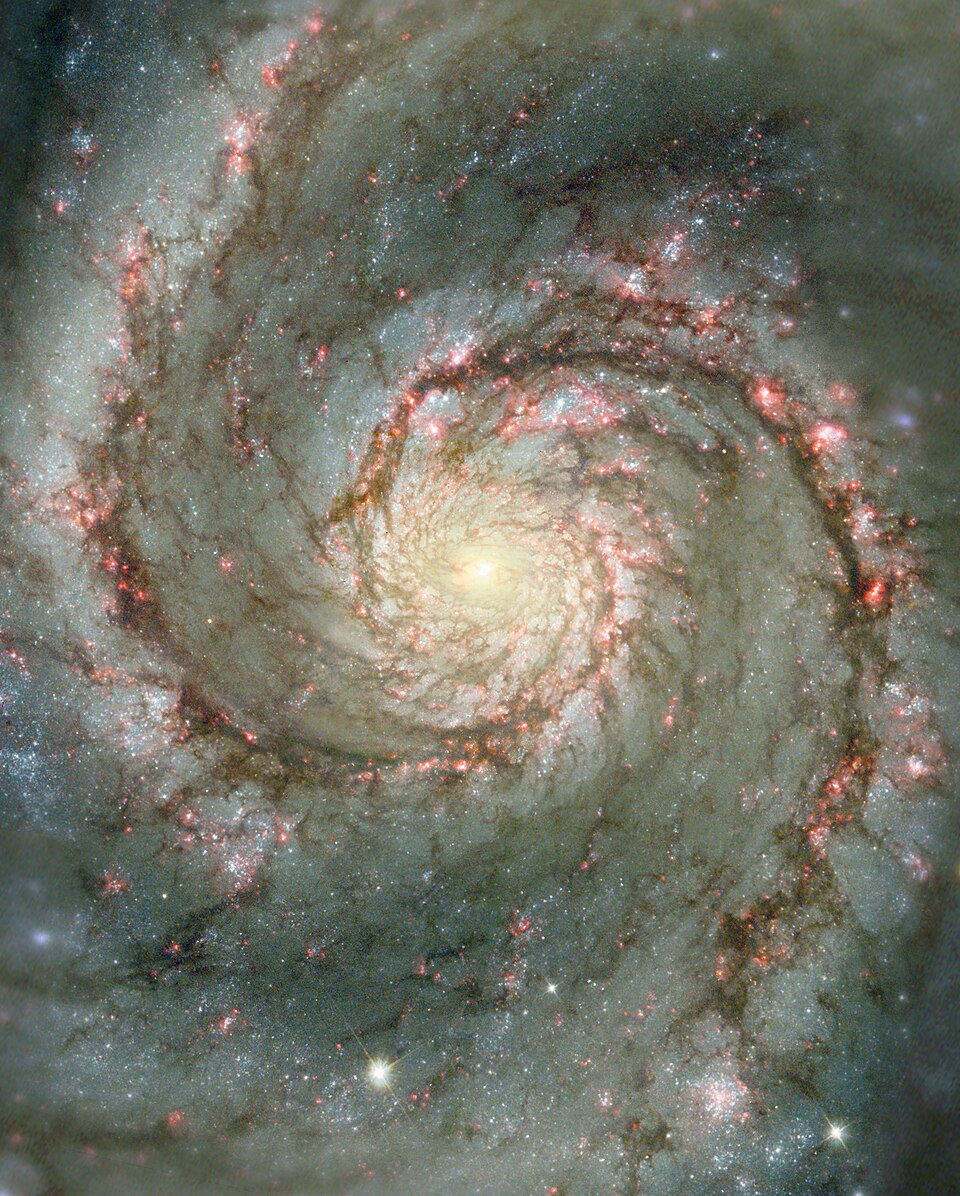
\includegraphics[width=0.7\columnwidth]{Whirpool_Galaxy-1.jpg}
		\caption{\footnotesize{\textbf{M51 Galaxy.} Crédit: Wikipédia.}}
	\end{figure}
	
	\begin{figure}[H]
		%\captionsetup{width=5cm}
		\centering
		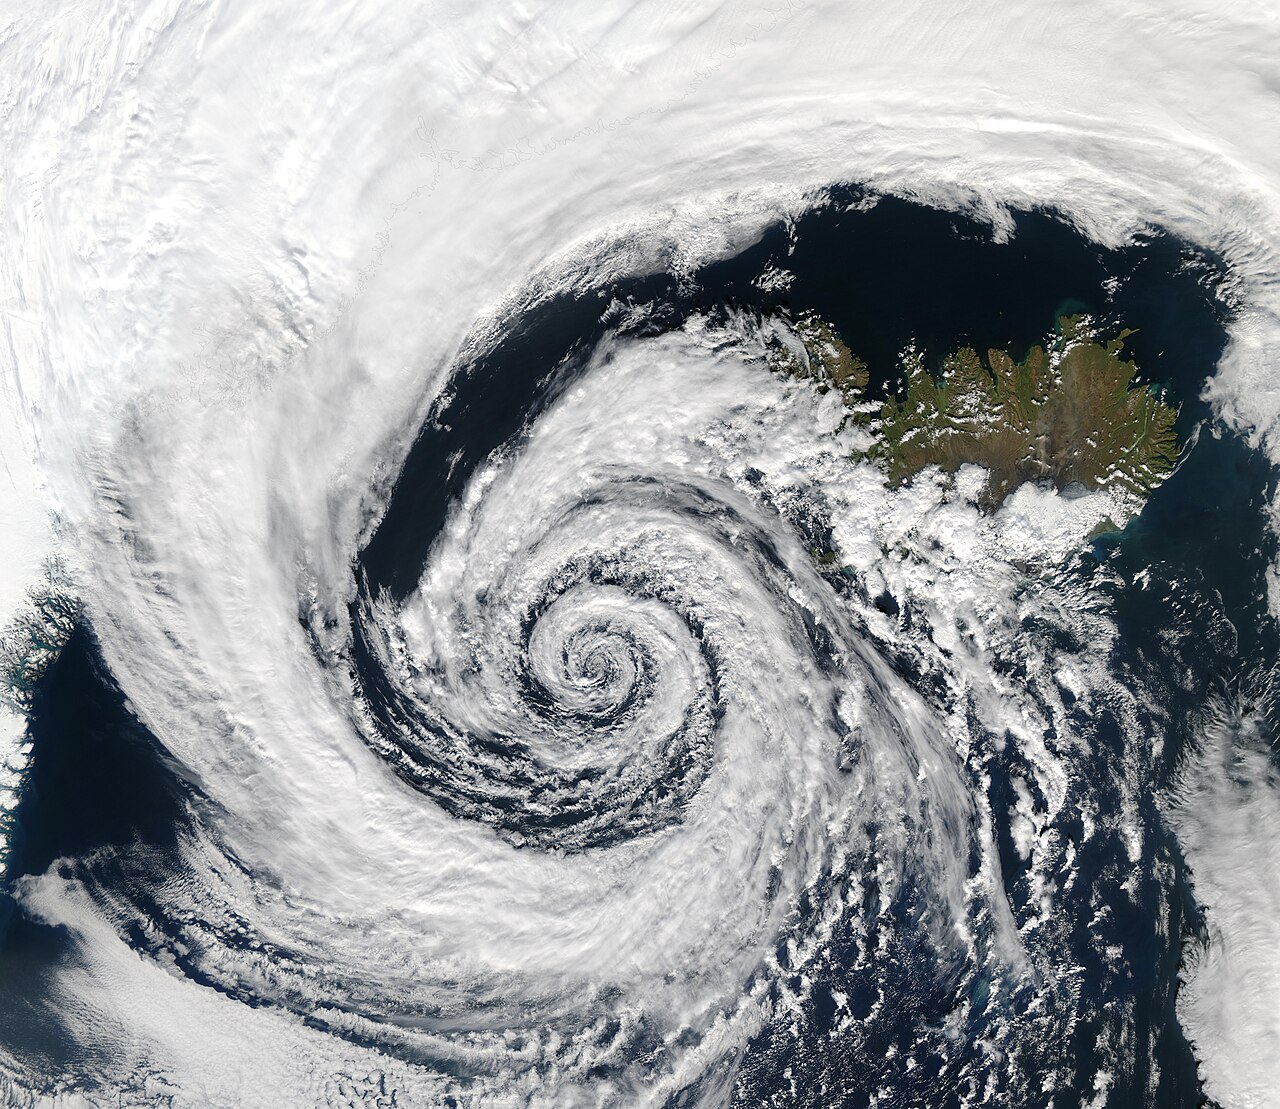
\includegraphics[width=0.8\columnwidth]{Low_pressure_system_over_Iceland-1.jpg}
		\caption{\footnotesize{\textbf{Low pressure system over Iceland.} Crédit: Wikipédia}}
	\end{figure}
	
	\begin{figure}[H]
		%\captionsetup{width=5cm}
		\centering
		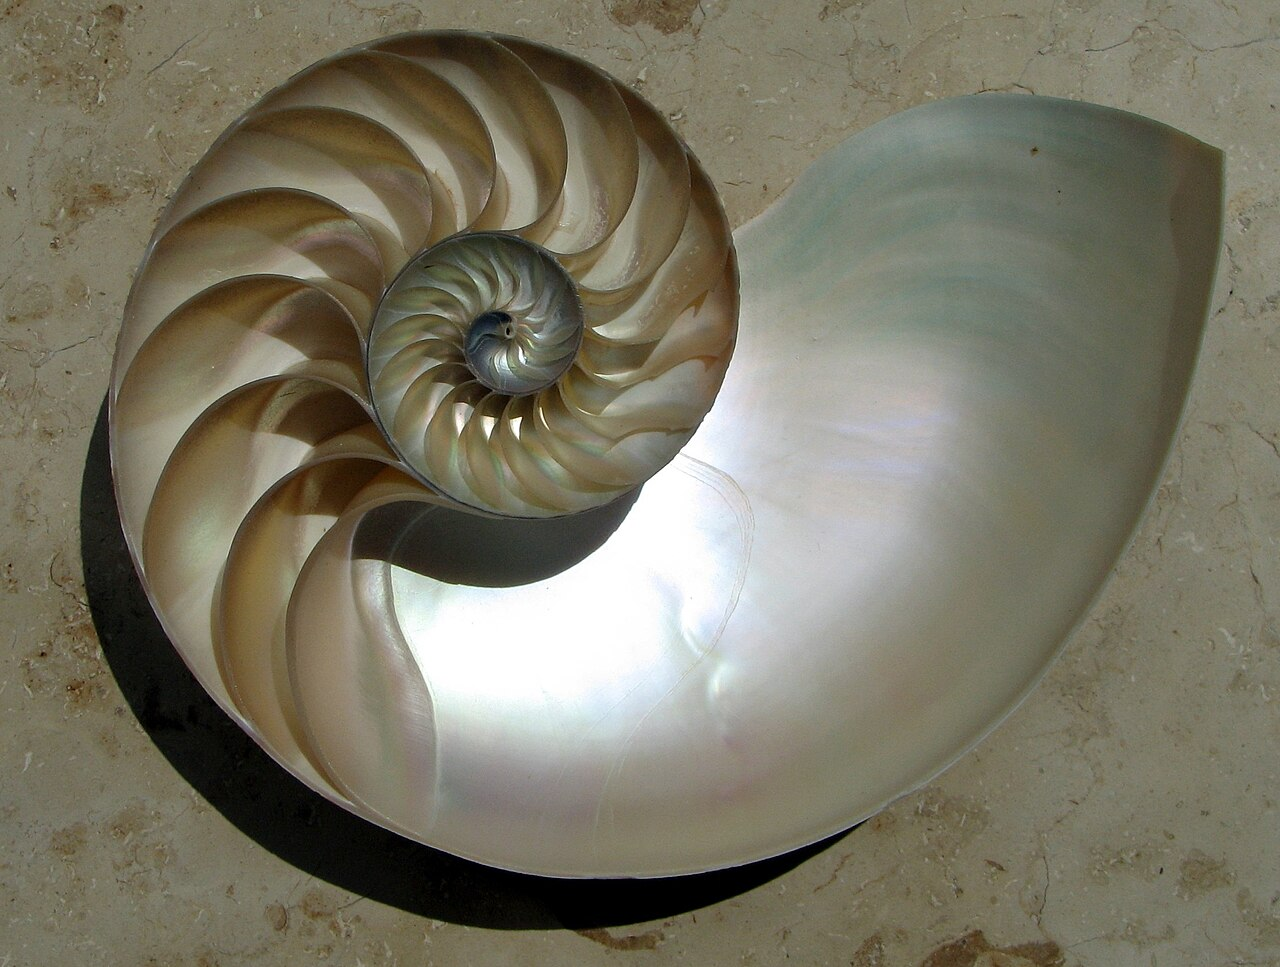
\includegraphics[width=0.9\columnwidth]{NautilusCutawayLogarithmicSpiral-1.jpg}
		\caption{\footnotesize{\textbf{Nautilus cutaway logarithmics spiral.} Crédit: Wikipédia}}
	\end{figure}
	
	\begin{figure}[H]
		%\captionsetup{width=5cm}
		\centering
		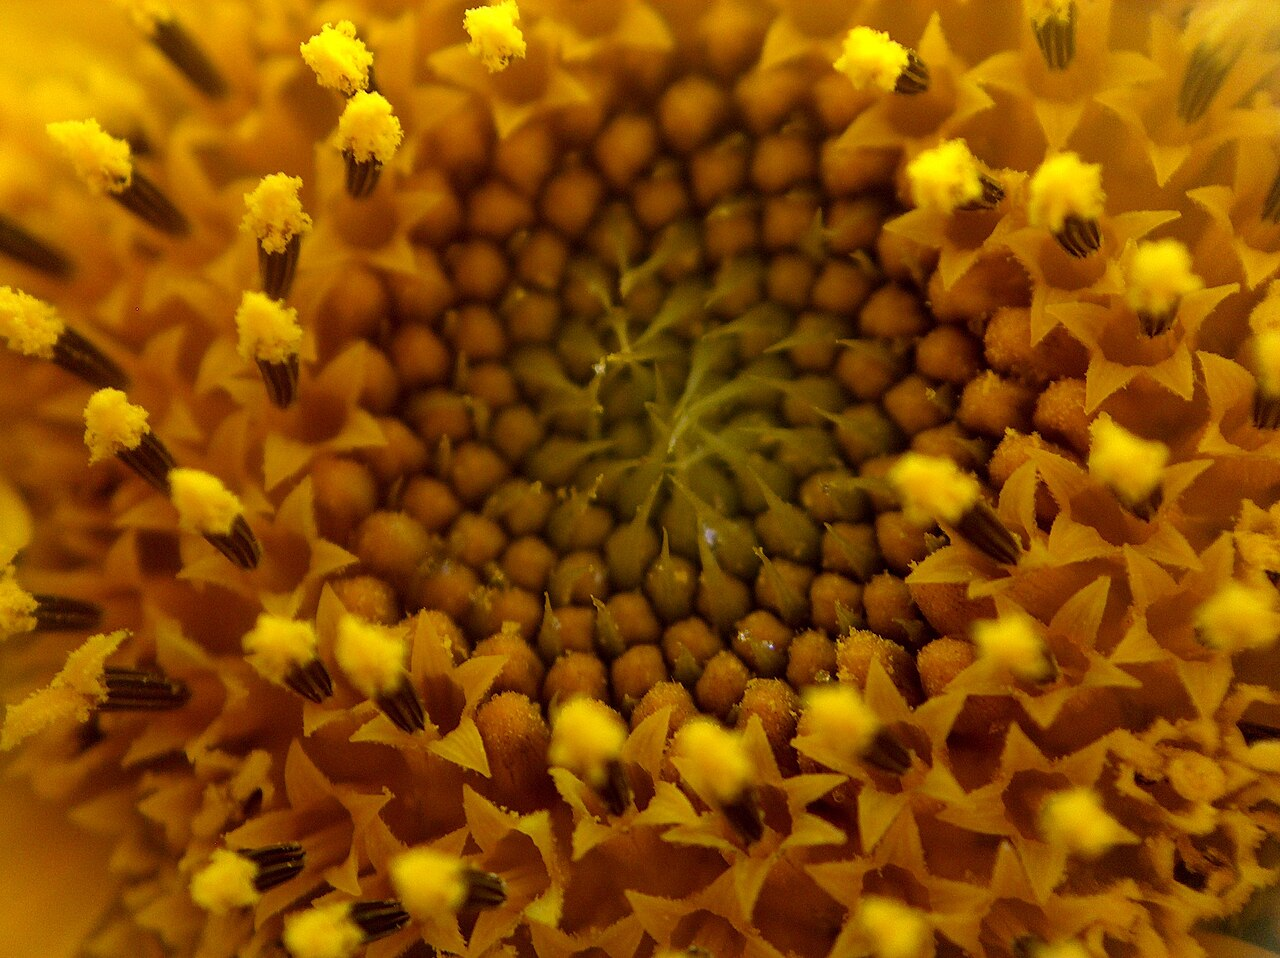
\includegraphics[width=0.9\columnwidth]{Close_up_Helianthus_annuus-2.jpg}
		\caption{\footnotesize{\textbf{Close up Helianthus annuus.} Crédit: Wikipédia}}
	\end{figure}
	
	
	Naturally, representations of the electron, neutrino, or atomic nuclei should be added later!
	
	But as much as nature tends toward the $S_3$ node — Bernoulli’s "admirable node" of the \textit{spira mirabilis} — it does not always succeed. The model sometimes deviates toward the Archimedean spiral, whose radius in this case has a constant increment. This form is found in some plants or certain vortex phenomena.
	
	In any case, nature is well managed by a Fibonacci-type fractal law of dimension 7, which could be named a "heptanacci" sequence, with a Pisano period of 7. As for the "Lucas sequence," it could represent the energy states of each of the nodes.
	
	It is therefore normal to find logarithmic spirals at all scales—the ultimate proof of the validity of \PQ.
	
	\subsection{Why life?}
	
	The question of the birth of life in a fundamental physics article may at first seem surprising, even absurd. But it is only so in appearance. Indeed, the Big Bang model of \PQ, and \PQ\ in general, puts determinism back at the center of physics. Given a specific condition (a cause), only one possible answer exists (the finality).
	
	Thus, the way the initial conditions of the universe were set—namely a left-handed rotation, a given energy, a constrained radius, and 7 degrees of freedom—generated the current universe without it being possible to change anything. Thus, matter was born according to an order, and this order gave a cosmological physics where no parameter arises from chance.
	
	Our Earth was thus born from this initial movement as an inevitable consequence of everything that preceded it. It is probable that a simple change in the placement of an atom at a cosmological time preceding the creation of the Earth would have resulted in a quite different universe: this is the butterfly effect on a cosmological scale.
	
	There is therefore no trace of chance left in the creative process that led to life on Earth.
	
	However, it must be noted that chance stops at the purely mechanical aspect of the creative process: as soon as a living object is created, the latter no longer follows a fractal law—at least it is capable of moving away from it in its specific behavior, even if general behavior always proceeds from a fusion to ensure the reproduction of the species \cite{queirosconde2003entropie}. Living things therefore only have a local impact on the general process at the scale of the universe.
	
	It must also be noted that life is a rupture in the creative process. In our universe, the stable mass node is of type $S_3$, i.e., a chiral node. The human species is not chiral, as if the node were exploiting its total capacities—a sort of super-synthesis of the entire initial process. From this point of view, it is possible to see the human species as the pinnacle, in the sense of maximal exploitation, of the universe's creative capacities.
	
	\section{Metaphysics of quantum plenodynamics}
	
	In the 16th century, Newton's introduction of mathematics into physics had a side effect: physics gave up metaphysics, since everything was mechanism. It sufficed to put the world into equations to explain it.
	
	It was quantum mechanics that reversed the trend four centuries later by introducing indeterminism because of its probabilistic basis. While the physicists of old were all trained in metaphysics, this was not—and still is no longer—the case today. We have since been entitled to a whole series of somewhat bizarre interpretations where everyone offered their own theory, from multiple universes to the intervention of the observer's consciousness: everything seemed possible, provided one gave up all logical spirit and elementary common sense.
	
	\PQ\ forcibly reintroduces absolute determinism. This unexpected return of determinism has two consequences. The first is to deconstruct all metaphysics based on the "quantum blur" of the last seventy years. The second could be a formidable leap back four centuries: everything has become mechanical again, close the book!
	
	But is it true? The model seems very robust and offers for the first time a coherent physics of everything, without a real hole. It can therefore be trusted.
	
	\textit{But what does it say in substance?}
	
	That at the origin of the world, there is a bivector. And what is a bivector, if not a pair of two objects linked so strongly that they are fusional? Is this not a very precise definition of the Holy Trinity? Two persons, the Father and the Son, are so linked that they gave birth to a third person, the Holy Spirit? \cite{aleteia_trinite_ref}
	
	The coincidence could stop there. But what do the Scriptures say? God the Father, the left vector, breathed (the energy) and sent His Son, the Word, placed at His right (the right vector, which thus passes in front of him by performing a leftward rotation), according to a process carried out in seven steps (\textit{cf}. Genesis \cite{aelf_genese1}). Are these not \textbf{exactly} the initial conditions?
	
	Let us continue and observe what the book of Genesis describes—which was long decried because of the alleged inversion of the order of the moments of creation. The Father begins by sending His breath at the initial step ($Cℓ_0$), the earth and the sky are created—a figuration of the two nested circles ($Cℓ_1$)—then light bursts forth (the famous "Fiat Lux") at $Cℓ_2$. Genesis is therefore perfectly in phase with the Big Bang model if, of course, the notion of "day" is replaced with the notion of fractal time from the model.
	
	Furthermore, we can see a wink from King David in Psalm 147, verse 15, which says: "He (the Lord) sends his word to the earth: His Word runs swiftly," \cite{aelf_psaume147} which is a very poetic way of synthesizing the process of Creation.
	
	Note that by fractal construction, everything is in the image of the initial bivector, therefore in the image of God.
	
	Finally, life is an inevitable consequence of the initial conditions: there is no chance in the appearance of life. If God is associated with the starting bivector, then life is indeed an initial will of God who set up the exact conditions for its appearance.
	
	Only life generates an indeterimistic rupture in the process, and this rupture is also explained in the Scriptures by free will. \cite{vatican_libre_arbitre}
	
	The only thing that \PQ\ does not explain is the soul. But if we trust the Scriptures, the soul would be in another dimension than our universe, therefore not describable by this theory, which makes this statement reasonable. Material man would be the most evolved node of Creation and his soul a gift from God: he would therefore be doubly and fully in the image of God (\textit{imago Dei}).
	
	It would however be possible to imagine what the invisible world could look like via \PQ. Indeed, in the Scriptures, there is always an association between the invisible world and light\cite{aleteia_lumiere_ref}. Christ is the Light of the world, angels are beings of light, and Lucifer is himself the luminous being par excellence. On the other hand, the description of a tunnel of light keeps recurring in near-death experiences. The invisible world is thus associated with light and it was created before the visible world. In the process of creation via \PQ, only two states can be associated with light: $Cℓ_2$ and $Cℓ_5$, which are photonic eras. $Cℓ_2$ is the pre-Planckian era, with few generated elements ($2^{32}$), which seems insufficient to populate the invisible world with "myriads of myriads of angels," a biblical expression designating an astronomical quantity. Only the $Cℓ_5$ era seems like a good candidate for this setting of creation. Indeed, its dimensions higher than $Cℓ_3$ and the impressive number of objects constituting its "plenum" allow it to generate—probably according to a process identical to our own, namely a screwing energy not sufficient to create the switch to $Cℓ_6$—all the beings of light of Creation. As for knowing how they communicate with our $Cℓ_3$ universe...
	
	Finally, it "suffices" for the original bivector to perform two screw turns to create both worlds in the same place: the first turn, much more energetic than the second, creates the universe of the invisible world, and the second turn allows for the creation of our world. The two worlds thus overlap, without it being necessary to create two different physics...
	
	To conclude by returning to physics, the breath—i.e., the initial energy—would correspond exactly to one of the conditions necessary for the creation of the universe. The fine-structure constant—the unique fine-tuning of the universe and perfect excess neutrino energy to generate electromagnetic interaction—could thus be considered as the constant of God.
	
	\section{Conclusion} 
	
	It is time to conclude. Quantum plenodynamics aims to be a theory of everything, and it has solid arguments to put forward. It still needs to pass the fire of peer review and have a complete mathematical development added to it. But before creating this base, it might be healthy to continue exploring its purely mechanical capacities to go to the end of the model, whose objective remains to be accessible to the greatest number. And above all, to remain a physical theory!
	
	In any case, \PQ\ has already achieved its first goal: presenting its physics "simply" so that all can integrate it, while preserving an ontological sense for physics.
	
	We must not forget Louis de Broglie in the process, many of whose ideas have been confirmed throughout this presentation. De Broglie was a visionary, and it is perhaps time to pay him the tribute and place he deserves. Physics must remain physics and mathematics a tool. He who confuses the object with the means ends up losing himself. He can be cited on this subject: "[...] We must never forget that these abstract representations [mathematical models] have no physical reality. Only the displacement of localized elements in space over time has physical reality. For this reason, the use of these representations is not without some dangers." \cite{debroglie1976physique}
	
	Finally, we can marvel at the mechanical beauty of \PQ: the simplicity of the model is matched only by its elegance. The fractal law is found everywhere and at all scales, from the plenum to cosmological immensity, like a permanent wink to researchers who had the solution under their noses all along.
	
	\section{Bibliography}
	\printbibliography
	
	\section{Source}
	\section*{Source of the document}
	
	%This article was published on the HAL platform (\url{https://hal.science/}) which linked it to arXiv (\url{https://arxiv.org/}).
	\medskip
	
	Here is the link to the original repository:
	\url{https://github.com/patricekaratchentzeff/plenodynamique-quantique}
	\medskip
	
	The document was compiled under Lua\LaTeX\ with the version \TeX Live 2023.20240207-1.
	
	This article is freely accessible and distributable under the CC BY license. This means you can do whatever you want with it, provided you cite the author.
	
	\section{Table of Contents}
	\tableofcontents
	\listoffigures
	\listoftables
\end{multicols}
	
	
\end{document}




































